% ===================================================================== main.tex
% FLOW BEHAVIOR AND THERMAL EFFECTS IN MULTIPHYSICS SYSTEMS
% Section 10B final internship engineering report - RE-ANALYSIS 2026
% Build: latexmk -pdf main.tex   (BIBINPUTS must include ../References)
\documentclass[10pt,a4paper,oneside,openany]{report}
% ===================================================================== preamble.tex
% Section 10B report - RE-ANALYSIS 2026
\usepackage[T1]{fontenc}
\usepackage[utf8]{inputenc}
\usepackage[sc]{mathpazo}
\usepackage[scaled=0.90]{helvet}
\usepackage{textcomp}
\usepackage[a4paper,left=20mm,right=20mm,top=20mm,bottom=20mm,headheight=14pt]{geometry}
\usepackage{amsmath,amssymb,mathtools,bm,upgreek}
\usepackage{graphicx}
\usepackage[labelfont={bf,sf},font=small,skip=4pt]{caption}
\usepackage[labelfont={bf,sf},font=small]{subcaption}
\usepackage{booktabs,array,tabularx,multirow,makecell,longtable}
\usepackage{siunitx}
\sisetup{group-separator={,},group-minimum-digits=4,per-mode=symbol}
\usepackage{xcolor}
\usepackage{enumitem}
\setlist{nosep,leftmargin=*,topsep=2pt}
\usepackage{microtype}
\usepackage{placeins}
\usepackage{multicol}
\usepackage{float}
\usepackage{titlesec}
\usepackage{fancyhdr}
\usepackage[numbers,square,sort&compress]{natbib}
\usepackage{tocloft}
\usepackage{etoolbox}
\usepackage[hidelinks]{hyperref}
\hypersetup{colorlinks=true,linkcolor=blue!40!black,citecolor=blue!40!black,urlcolor=blue!40!black,
  pdftitle={Flow Behavior and Thermal Effects in Multiphysics Systems},
  pdfauthor={Rohan Balram Patel},
  pdfsubject={CFD, conjugate heat transfer and thermo-structural analysis of a heated cylindrical duct},
  pdfkeywords={CFD, conjugate heat transfer, ANSYS Fluent, ANSYS Mechanical, thermal stress, linear buckling, Eleation internship}}

\graphicspath{{../Figures/}}
\definecolor{recon}{RGB}{150,40,30}
\definecolor{boxbg}{RGB}{246,243,236}

% headings
\titleformat{\chapter}[hang]{\sffamily\bfseries\LARGE}{\thechapter}{0.8em}{}[\vspace{2pt}\titlerule]
\titlespacing*{\chapter}{0pt}{6pt}{10pt}
% chapters run on without a forced page break (compact report layout)
\makeatletter\patchcmd{\chapter}{\if@openright\cleardoublepage\else\clearpage\fi}{\par\FloatBarrier\vspace{8pt}}{}{}\makeatother
\titleformat{\section}{\sffamily\bfseries\large}{\thesection}{0.7em}{}
\titleformat{\subsection}{\sffamily\bfseries\normalsize}{\thesubsection}{0.6em}{}
\titlespacing*{\section}{0pt}{9pt plus 2pt minus 2pt}{4pt plus 1pt}
\titlespacing*{\subsection}{0pt}{7pt plus 2pt minus 2pt}{3pt plus 1pt}
\setcounter{secnumdepth}{2}
\setcounter{tocdepth}{1}

% header / footer
\pagestyle{fancy}
\fancyhf{}
\fancyhead[L]{\sffamily\footnotesize Flow Behavior and Thermal Effects in Multiphysics Systems}
\fancyhead[R]{\sffamily\footnotesize Eleation internship, February--May 2025}
\fancyfoot[C]{\sffamily\footnotesize\thepage}
\renewcommand{\headrulewidth}{0.4pt}
\fancypagestyle{plain}{\fancyhf{}\fancyfoot[C]{\sffamily\footnotesize\thepage}\renewcommand{\headrulewidth}{0pt}}

% lists of figures / tables
\renewcommand{\cftfigfont}{\small}
\renewcommand{\cfttabfont}{\small}
\renewcommand{\cftfigpagefont}{\small}
\renewcommand{\cfttabpagefont}{\small}
\setlength{\cftbeforefigskip}{1pt}
\setlength{\cftbeforetabskip}{1pt}
\setlength{\cftbeforechapskip}{4pt}

% floats
\renewcommand{\topfraction}{0.9}
\renewcommand{\bottomfraction}{0.8}
\renewcommand{\textfraction}{0.07}
\renewcommand{\floatpagefraction}{0.8}
\setcounter{topnumber}{3}
\setcounter{bottomnumber}{2}
\setcounter{totalnumber}{4}
\setlength{\parskip}{2pt plus 1pt}
\setlength{\parindent}{0pt}

% helper macros
\newcommand{\diameter}{\text{\O}}
\newcommand{\lamone}{\ensuremath{\lambda_1}}
\newcommand{\degC}{\,\textdegree C}
\newcommand{\src}[1]{\par\vspace{1pt}{\footnotesize\itshape #1}}
\newcommand{\provmech}{ANSYS Mechanical image export (\texttt{Graphics.ExportImage}) of the solved result object, unedited.}
\newcommand{\provcfd}{Plotted with matplotlib from data exported from the converged ANSYS Fluent solution; not a GUI screenshot.}
\newcommand{\provmesh}{matplotlib render of the actual mesh arrays read by Fluent; not an ANSYS GUI screenshot.}
\newcommand{\provcad}{Rendered from the geometry exported by ANSYS SpaceClaim; not a GUI screenshot.}
\newcommand{\provdata}{Plotted with matplotlib from the solver output tables of this project.}
\newcommand{\recbox}[1]{\par\smallskip\noindent\fcolorbox{recon}{boxbg}{\parbox{\dimexpr\linewidth-2\fboxsep-2\fboxrule}{\small #1}}\par\smallskip}

\renewcommand{\bibname}{References}
\setlength{\textfloatsep}{10pt plus 2pt minus 3pt}
\setlength{\floatsep}{8pt plus 2pt minus 2pt}
\setlength{\intextsep}{8pt plus 2pt minus 2pt}
\setlength{\emergencystretch}{3em}
\assignpagestyle{\chapter}{fancy}
\setlength{\bibsep}{1.5pt plus 0.5pt}


\begin{document}
\pagenumbering{alph}   % cover page gets its own anchor (avoids a duplicate "page.i" destination)
% ===================================================================== front matter
% ---------------------------------------------------------------- 1. cover page
\begin{titlepage}
\thispagestyle{empty}
\centering
\vspace*{8mm}
{\sffamily\large INTERNSHIP ENGINEERING REPORT\par}
\vspace{18mm}
{\sffamily\bfseries\Huge FLOW BEHAVIOR AND THERMAL EFFECTS IN MULTIPHYSICS SYSTEMS\par}
\vspace{10mm}
{\sffamily\Large CFD, Conjugate Heat Transfer and Thermo-Structural Analysis of a Heated Cylindrical Duct\par}
\vspace{16mm}
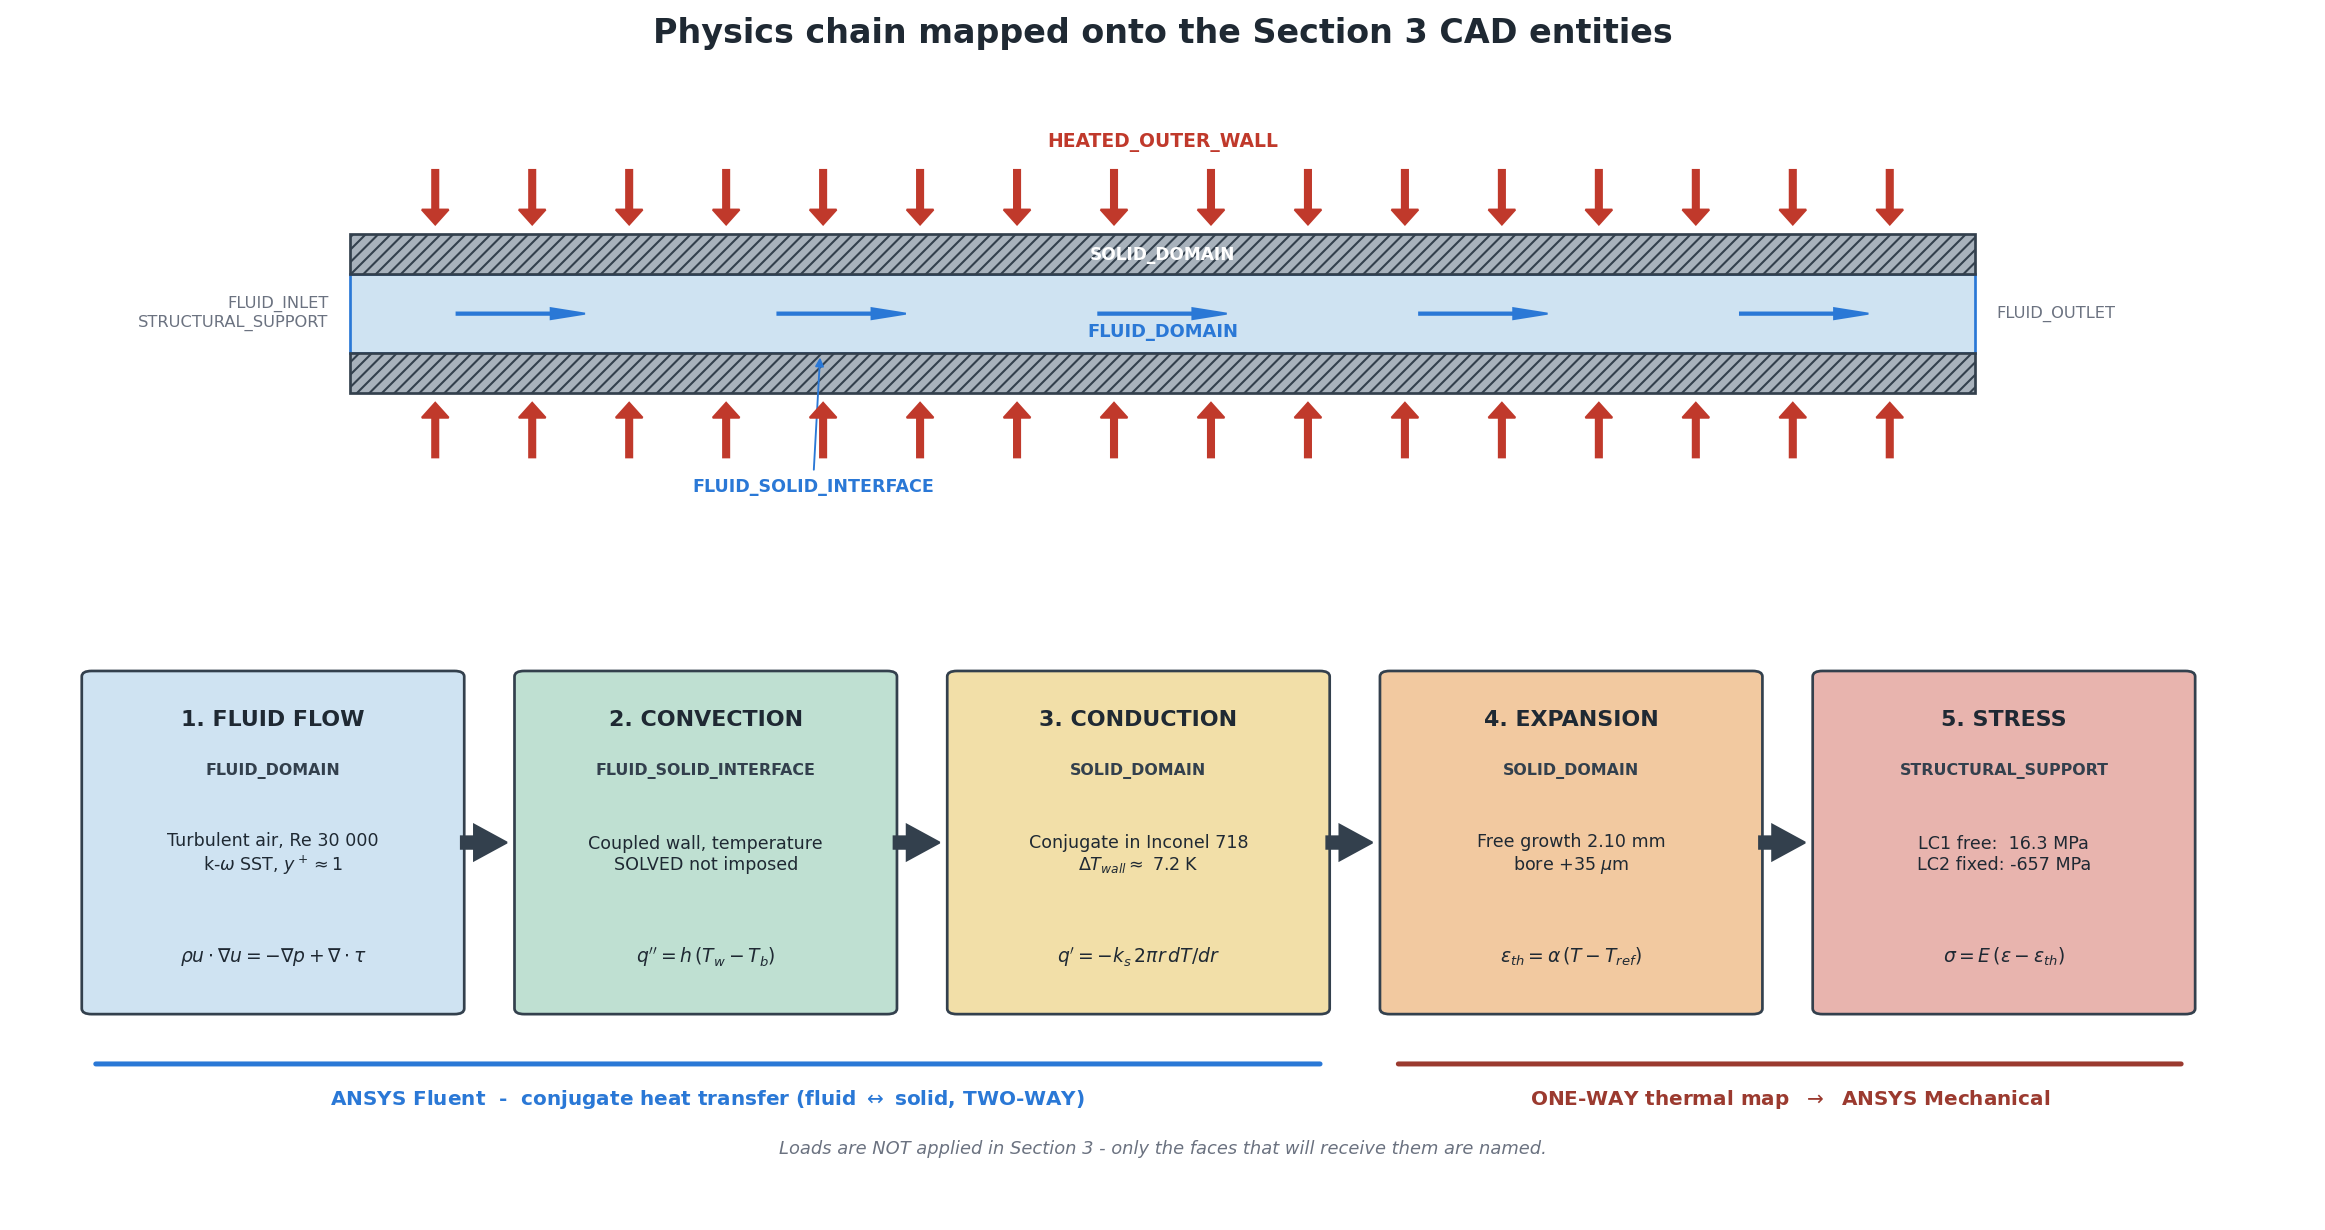
\includegraphics[width=0.78\linewidth]{PHYSICS_SCHEMATIC.png}\par
{\footnotesize\itshape Physics chain of the model (Section 3 drawing; values printed in the process boxes are Section 2 analytical estimates).\par}
\vspace{14mm}
{\large Rohan Balram Patel\par}
{\normalsize B.Tech Aerospace Engineering, Dayananda Sagar University, Bengaluru\par}
\vspace{6mm}
{\normalsize Eleation\par}
{\normalsize Internship: February--May 2025\par}
\vspace{10mm}
{\sffamily\small Numerical analysis using ANSYS Workbench, ANSYS Fluent and ANSYS Mechanical\par}
\vfill
\end{titlepage}
\pagenumbering{roman}

% ---------------------------------------------------------------- 2./3. internship information and project title
\chapter*{Internship Information}
\addcontentsline{toc}{chapter}{Internship Information}
\begin{tabular}{@{}>{\bfseries}p{0.30\linewidth}p{0.64\linewidth}@{}}
Engineer & Rohan Balram Patel \\
Programme & B.Tech Aerospace Engineering, Dayananda Sagar University, Bengaluru \\
Organisation & Eleation \\
Internship period & February 2025 -- May 2025 \\
Tools & ANSYS Workbench (SpaceClaim), ANSYS Fluent, ANSYS Mechanical / MAPDL; Python 3.10 (bundled with ANSYS) for calculations and post-processing \\
Report status & Final internship engineering report
\end{tabular}

\section*{Project Title}
\textbf{Flow Behavior and Thermal Effects in Multiphysics Systems}\\
CFD, Conjugate Heat Transfer and Thermo-Structural Analysis of a Heated Cylindrical Duct

% ---------------------------------------------------------------- 4. declaration / note on the analysis record
\chapter*{Declaration}
\addcontentsline{toc}{chapter}{Declaration}
\recbox{\textbf{Note on the analysis record.} The original internship project files were not retained. The geometry, operating
parameters, simulation set-up and numerical results presented in this report therefore come from a complete re-analysis of the
internship problem, carried out after the internship with ANSYS Workbench, Fluent and Mechanical and based on the documented project
scope. They are not copies of the original internship analysis.}

Only documented internship information (engineer, programme, organisation, period and tool set) is described as historical fact.
Every other value in this report is labelled with one of the following terms:

\begin{itemize}
\item \textbf{Selected} -- an input value chosen for this study with a stated rationale (for example $D_i$ = 20~mm, $V_{in}$ = 23.5~m/s, $q''$ = 8000~W/m$^2$, Inconel 718);
\item \textbf{Assumed} -- an engineering idealisation (for example steady state, uniform heat flux, $\nu$ = 0.294, idealised supports);
\item \textbf{Calculated} -- a hand or script calculation from the selected inputs (the Section 2 analytical baseline);
\item \textbf{Simulated} -- the output of an ANSYS solution of this project.
\end{itemize}

No experimental or measured data exist for this project, and none has been created. Verification is against analytical theory,
published correlations and internal consistency checks; the results are therefore verified but not experimentally validated.

\textbf{Declaration.} This report presents the analysis as documented in the project record (the file
\texttt{PROJECT\_STATE.md}, Sections 0--10A) and in the audited master dataset of Section 10A
(\texttt{MASTER\_PROJECT\_DATA.csv}). Every numerical result quoted is a
calculation or simulation of the analysed problem and is traceable to a project file. No original company procedure, supervisor
comment or original screenshot is reproduced or implied.

\vspace{6mm}
Rohan Balram Patel

% ---------------------------------------------------------------- 5. acknowledgement
\clearpage   % keeps the original page break (Acknowledgement and Abstract on page ii)
\chapter*{Acknowledgement}
\addcontentsline{toc}{chapter}{Acknowledgement}
I thank Eleation for the internship opportunity between February and May 2025, during which the project on flow behaviour and
thermal effects in multiphysics systems was carried out, and the Department of Aerospace Engineering of Dayananda Sagar University,
Bengaluru, for the academic framework of the internship. The analysis documented here relied on ANSYS Workbench, Fluent and Mechanical
and on the published data and correlations listed in the references.

% ---------------------------------------------------------------- 6. abstract
\chapter*{Abstract}
\addcontentsline{toc}{chapter}{Abstract}
This report presents the Eleation internship project \emph{Flow Behavior and Thermal Effects in Multiphysics Systems}
(February--May 2025): a numerical analysis using ANSYS Workbench, ANSYS Fluent and ANSYS Mechanical. The system is an air-cooled,
externally heated Inconel 718 duct (20/40~mm inner/outer diameter, 600~mm long).

An analytical baseline preceded all simulations. Turbulent internal flow and conjugate heat transfer were solved in ANSYS Fluent (steady,
$k$--$\omega$ SST, wall-resolved) at 23.5~m/s and 300~K inlet with an outer-wall heat flux of 8000~W/m$^2$. On the 159,840-cell
medium mesh the converged solution gives a pressure drop of 438.13~Pa, an outlet bulk temperature of 368.93~K and a maximum
solid temperature of 562.58~K, with only 7.58~K across the wall at mid-span. A three-mesh study shows approximately convergent behaviour
(fine mesh 560.83~K; extrapolated 558.13~K).

The solid temperature field was transferred one-way to ANSYS Mechanical (mapping error $\le$ 0.081~K). Free expansion gives 1.84~mm
growth and a 24.28~MPa peak von Mises stress. Full axial restraint gives a 548.94~kN end force, a mean axial stress of $-$582.44~MPa and
a local peak of 605.16~MPa, 57.8\,\% of the local yield strength; structural mesh effects are below
$5\times10^{-4}$. Linear eigenvalue buckling under the baseline S1 support gives $\lambda_1$ = 1.108, below the first-yield factor of 1.730,
while alternative idealised supports give 2.232 (S3) and 4.300 (S2). A one-factor parametric study (velocity and heat flux $\pm$10\,\%,
wall thickness 8 and 12~mm), with full solutions of every case, shows that velocity acts mainly on cooling and pressure drop,
heat flux drives temperature and stress, and thickness drives stiffness and buckling capacity; $\lambda_1$ falls below 1 for +10\,\% heat
flux and the 8~mm wall. An additional geometrically nonlinear analysis with ANSYS LS-DYNA, performed as an extension with mode-shaped
numerical imperfections of 0.1, 0.6 and 1.2~mm, gives Southwell characteristic-load estimates of 607.7--612.3~kN, close to the linear
critical load of 608.25~kN, while lateral deflection and stress grow strongly with the imperfection amplitude.

The results are not validated against measurement. The real end restraint, measured geometric imperfections and
inelastic behaviour, the dominant open uncertainties, were not modelled. The study therefore characterises the thermal-stress mechanism and its sensitivities, not the
structural adequacy of a real component.

% ---------------------------------------------------------------- 7.-9. contents and lists
\cleardoublepage
\chapter*{Contents}
\addcontentsline{toc}{chapter}{Contents}
{\small\makeatletter\setlength{\columnsep}{8mm}\begin{multicols}{2}\@starttoc{toc}\end{multicols}\makeatother}
\clearpage
\phantomsection
\addcontentsline{toc}{chapter}{List of Figures}
{\sffamily\bfseries\LARGE List of Figures\par}\vspace{2pt}\hrule\vspace{8pt}
{\makeatletter\let\origaddvspace\addvspace\renewcommand{\addvspace}[1]{\origaddvspace{2pt}}\@starttoc{lof}\makeatother}
\vspace{14pt}
\phantomsection
\addcontentsline{toc}{chapter}{List of Tables}
{\sffamily\bfseries\LARGE List of Tables\par}\vspace{2pt}\hrule\vspace{8pt}
{\makeatletter\let\origaddvspace\addvspace\renewcommand{\addvspace}[1]{\origaddvspace{2pt}}\@starttoc{lot}\makeatother}

% ---------------------------------------------------------------- 10. abbreviations
\vspace{10pt}
\noindent\begin{minipage}{\linewidth}
\phantomsection
\addcontentsline{toc}{chapter}{List of Abbreviations and Symbols}
{\sffamily\bfseries\LARGE List of Abbreviations and Symbols\par}\vspace{2pt}\hrule\vspace{6pt}
{\footnotesize
\begin{tabular}{@{}p{0.10\linewidth}p{0.32\linewidth}p{0.12\linewidth}p{0.38\linewidth}@{}}
\toprule
\multicolumn{2}{@{}l}{\textbf{Abbreviations}} & \multicolumn{2}{l}{\textbf{Symbols}} \\
\midrule
CAD & computer-aided design & $A$, $I$ & section area [m$^2$]; second moment of area [m$^4$] \\
CFD & computational fluid dynamics & $c_p$ & specific heat [J/(kg\,K)] \\
CHT & conjugate heat transfer & $D_i$, $D_o$, $D_h$ & inner, outer, hydraulic diameter [m] \\
FE, FV & finite element, finite volume & $E$, $\nu$ & Young's modulus [Pa]; Poisson's ratio [--] \\
GCI & grid convergence index & $f$ & Darcy friction factor [--] \\
LC1 & load case 1, free expansion & $h$ & heat-transfer coefficient [W/(m$^2$\,K)] \\
LC2 & load case 2, axially restrained (S1) & $k$, $k_s$ & conductivity of air, of the solid [W/(m\,K)] \\
LC2P & LC2 with bore pressure & $K$, $L$ & effective-length factor [--]; length [m] \\
MAPDL & Mechanical APDL solver & $\dot m$, $N$ & mass flow rate [kg/s]; axial end force [N] \\
OQ & orthogonal quality & $Nu$, $Pr$, $Re$ & Nusselt, Prandtl, Reynolds numbers \\
P00 & official baseline case & $P_{cr}$ & critical buckling load [N] \\
RANS & Reynolds-averaged Navier--Stokes & $q''$, $Q$ & heat flux [W/m$^2$]; heat-transfer rate [W] \\
SST & shear-stress transport & $r$, $t$ & radius, radius of gyration [m]; wall thickness [m] \\
S1--S3 & support scenarios (Table~\ref{tab:supports}) & $S_y$ & 0.2\,\% proof (yield) strength [Pa] \\
TI & turbulence intensity & $T$, $T_{ref}$ & temperature, stress-free reference [K] \\
VM & von Mises (equivalent) stress & $y^+$ & dimensionless wall distance [--] \\
V01, V03 & velocity cases & $\alpha$ & thermal expansion coefficient [1/K] \\
Q01, Q03 & heat-flux cases & $\lambda_1$ & first linear buckling load factor [--] \\
T01, T03 & wall-thickness cases & $\mu$, $\rho$ & dynamic viscosity [Pa\,s]; density [kg/m$^3$] \\
1-D & one-dimensional & $\sigma_{vM}$, $\bar\sigma_z$ & von Mises stress; mean axial stress [Pa] \\
\bottomrule
\end{tabular}}
\end{minipage}


\cleardoublepage
\pagenumbering{arabic}
% ===================================================================== Chapter 1
\chapter{Introduction}\label{ch:intro}

\section{Background}
The internship project \emph{Flow Behavior and Thermal Effects in Multiphysics Systems} was carried out at Eleation between February and
May 2025 with ANSYS Workbench, Fluent and Mechanical. Its original files were not retained, so the analysis reported here was carried
out again after the internship: a representative multiphysics problem was defined, solved and audited from first principles, with every
input labelled as selected or assumed and every result traceable to a calculation or simulation in the project record. The note on the
analysis record at the front of the report states this formally; it applies to every number in the following chapters.

\section{Multiphysics Engineering Problems}
Many aerospace and energy components are loaded by several interacting physical processes at once. A heated duct, a combustor liner or
a heat-exchanger tube carries a flow that sets the convective boundary condition, the convective boundary condition sets the wall
temperature, and the wall temperature sets thermal strain and, where that strain is prevented, thermal stress. Each link has its own
governing equations and numerical methods, and the uncertainty of the final structural quantity depends on every link in the chain.

\section{Importance of Coupled Flow and Thermal Analysis}
In a conjugate problem the wall temperature is part of the solution rather than a boundary condition. Its accuracy depends on how well
the near-wall flow is resolved, because the air-side film usually carries most of the thermal resistance. A prescribed wall temperature
or an assumed heat-transfer coefficient would decouple the structural result from the flow physics that actually determines it.
Conjugate heat transfer (CHT) with a wall-resolved turbulence model therefore forms the thermal basis of this study.

\section{Motivation}
The study has two purposes. The first is technical: to demonstrate a complete and auditable simulation chain from flow to
structural stability, including verification at each step (analytical baseline, conservation checks, mesh studies, mapping checks).
The second is documentary: to provide a reproducible and auditable record of the internship problem, in which the status of every
value is stated explicitly.

\section{Problem Statement}
An air-cooled Inconel 718 duct is heated uniformly on its outer surface. The central question is:
\begin{quote}
\emph{Does thermal stress in the heated duct come mainly from the temperature gradient through the wall, or from restraint of the
duct's overall thermal growth -- and what are the consequences of that restraint for stability?}
\end{quote}
Answering it requires the flow field and heat-transfer coefficient, the conjugate temperature field in the wall, the thermal stresses for
free and restrained expansion, and the linear stability of the restrained duct, together with their sensitivity to the operating
conditions, the wall thickness and the end supports.

\section{Scope}
The study covers a steady-state, one-way coupled chain: Fluent CFD with conjugate heat transfer, transfer of the converged solid
temperature field to Mechanical, linear static analysis of two load cases (LC1 free expansion, LC2 axially restrained), linear
eigenvalue buckling on the LC2 pre-stress, a one-factor-at-a-time parametric study and a support-sensitivity study. Outside the scope are:
\begin{itemize}
\item transient start-up and thermal cycling;
\item radiation;
\item two-way fluid--structure coupling;
\item geometric or material nonlinearity and imperfection-sensitive buckling;
\item experimental validation.
\end{itemize}
These exclusions are revisited as limitations in Chapter~\ref{ch:unc} and as future work in Chapter~\ref{ch:future}. An additional
geometrically nonlinear, elastic buckling analysis with ANSYS LS-DYNA, performed as an extension of the thermo-structural analysis, is
reported separately in Section~\ref{sec:lsdyna}; it does not change the scope or the results of the main study.

\section{Objectives}
\begin{enumerate}
\item Define a representative heated-duct problem and an independent analytical baseline before any simulation.
\item Solve the turbulent flow and conjugate heat transfer in ANSYS Fluent to a converged, conservative solution with a resolved wall.
\item Quantify the CFD discretisation error with a three-mesh study and select the mesh for the structural phase.
\item Transfer the solid temperature field to ANSYS Mechanical and verify the transfer.
\item Compute thermal stress and deformation for free and restrained expansion and check structural mesh sensitivity.
\item Evaluate the linear buckling behaviour of the restrained duct and its dependence on the end supports.
\item Quantify the effect of inlet velocity, heat flux and wall thickness with actual CFD, structural and buckling solutions.
\item Record every uncertainty separately and state which conclusions the evidence supports.
\end{enumerate}

% ===================================================================== Chapter 2
\chapter{Engineering System}\label{ch:system}

\section{System Description}
The system is a straight, thick-walled circular duct of Inconel 718 with air flowing through its bore. A uniform heat flux enters the outer
surface, conducts through the wall and is removed by the turbulent air flow. The end faces are adiabatic. Structurally, the duct either
expands freely (LC1) or is held axially at both ends (LC2), in which case the prevented thermal growth produces an axial compressive
force. All dimensions and loads are selected class-B inputs (Chapter~\ref{ch:params}).

\section{Heated Duct Geometry}
Figure~\ref{fig:drawing} shows the dimensioned drawing prepared in Section 3 of the project. The bore diameter of 20~mm and the length of
600~mm give $L/D_i$ = 30, long enough for the flow to become hydrodynamically developed over the rear part of the duct. The diameter ratio
$D_o/D_i$ = 2 produces a 10~mm wall, thick enough for a measurable through-wall temperature difference and for a stiff column section.

\begin{figure}[htbp]
\centering
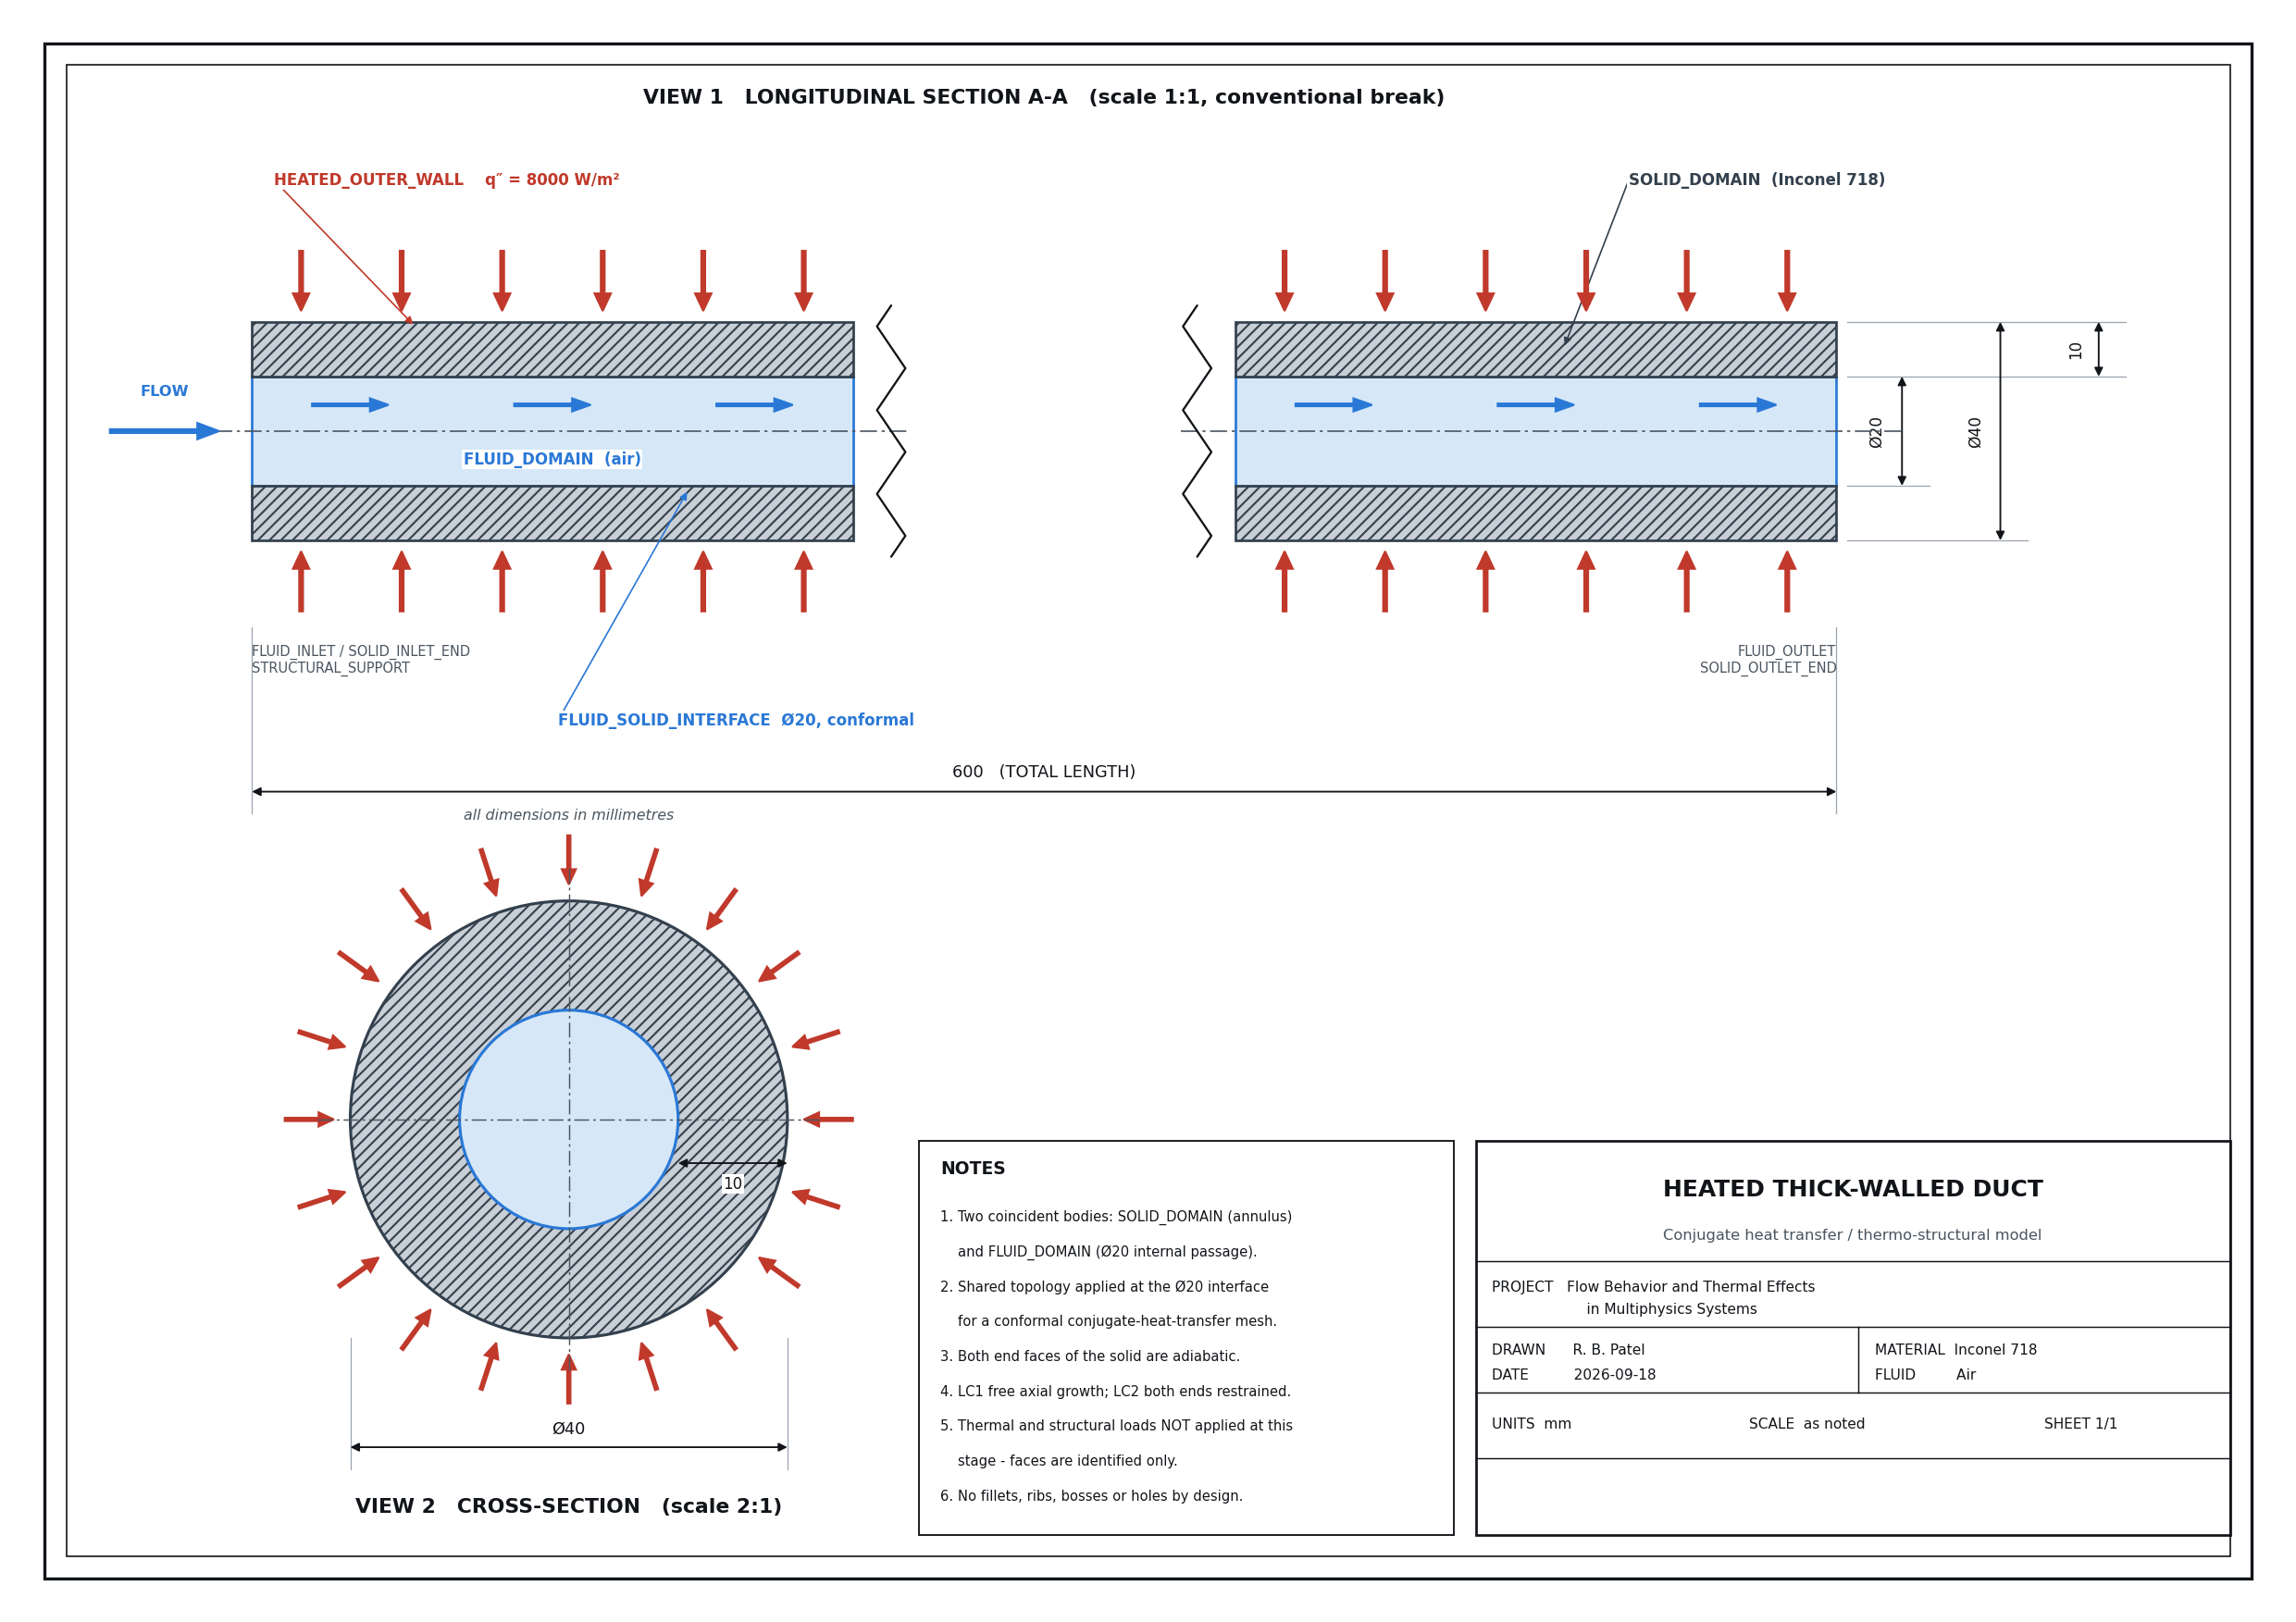
\includegraphics[width=0.74\linewidth]{ENGINEERING_DRAWING.png}
\caption[Engineering drawing of the heated duct]{Engineering drawing of the heated duct: longitudinal section and cross-section (dimensions in mm).}
\label{fig:drawing}
\src{Source: \texttt{03\_CAD\_Geometry/Drawings/ENGINEERING\_DRAWING.png} (project drawing of the analysed duct).}
\end{figure}

\section{Geometry Parameters}
Table~\ref{tab:geometry} lists the geometry. The heated area differs between the true cylinder and the CFD mesh, because the CFD section is
an inscribed 48-sided polygon; the resulting 0.071\,\% difference in heat input is exact and is discussed in Chapters~\ref{ch:cfdres}
and~\ref{ch:mi}.

%% generated by gen_tables.py - RE-ANALYSIS 2026
\begin{table}[htbp]
\centering
\small
\caption{Duct geometry of the baseline (selected class-B inputs, verified in the CAD model)}
\label{tab:geometry}
\begin{tabular}{>{\raggedright\arraybackslash}p{0.42\linewidth}lrl}
\toprule
Parameter & Symbol & Value & Unit \\
\midrule
Inner (bore) diameter & $D_i$ & 20 & mm \\
Outer diameter & $D_o$ & 40 & mm \\
Wall thickness & $t$ & 10 & mm \\
Length & $L$ & 600 & mm \\
Hydraulic diameter & $D_h$ & 20 & mm \\
Slenderness of the flow passage & $L/D_i$ & 30 & -- \\
Diameter ratio & $D_o/D_i$ & 2 & -- \\
Fluid flow area & $A_c$ & 314.159 & mm$^2$ \\
Solid volume & $V_s$ & $5.654867\times10^{-4}$ & m$^3$ \\
Heated outer area, true cylinder & $A_o$ & 0.07539822 & m$^2$ \\
Heated outer area, CFD 48-facet polygon & $A_{o,48}$ & 0.07534441 & m$^2$ \\
\bottomrule
\end{tabular}
\par\smallskip\parbox{\linewidth}{\footnotesize\raggedright Source: \texttt{MASTER\_PROJECT\_DATA.csv} rows M023--M031 (CAD values from \texttt{cad\_measurements.json}; the 48-facet area from the Fluent surface-integral report). Status VERIFIED.}
\end{table}


\section{Fluid Domain}
The fluid domain is a solid body filling the bore ($\diameter$20~mm $\times$ 600~mm, volume $1.884956\times10^{-4}$ m$^3$). Air enters
through \texttt{FLUID\_INLET} at $z = 0$ and leaves through \texttt{FLUID\_OUTLET} at $z$ = 600~mm; its only lateral boundary is the
fluid--solid interface.

\section{Solid Domain}
The solid domain is the Inconel 718 annulus between $r$ = 10~mm and $r$ = 20~mm (volume $5.654867\times10^{-4}$ m$^3$, mass 4.631 kg). Its outer
cylinder carries the heat flux; its inner cylinder is the conjugate interface; its end annuli are adiabatic and, in the structural model,
carry the axial supports.

\section{Heat-Transfer Path}
Heat follows a single series path (Figure~\ref{fig:physics}): conduction radially inward through the wall, convection from the bore
surface into the air, and advection of the absorbed energy to the outlet. The analytical baseline shows that the conduction resistance of
the wall is only 3.4\,\% of the total resistance between outer wall and air; the air film carries the remaining 96.6\,\%
($R_{cond}/R_{conv}$ = 0.0342). The metal temperature is therefore controlled mainly by the heat-transfer coefficient on the air side, not by
the conductivity of the wall.

\begin{figure}[htbp]
\centering
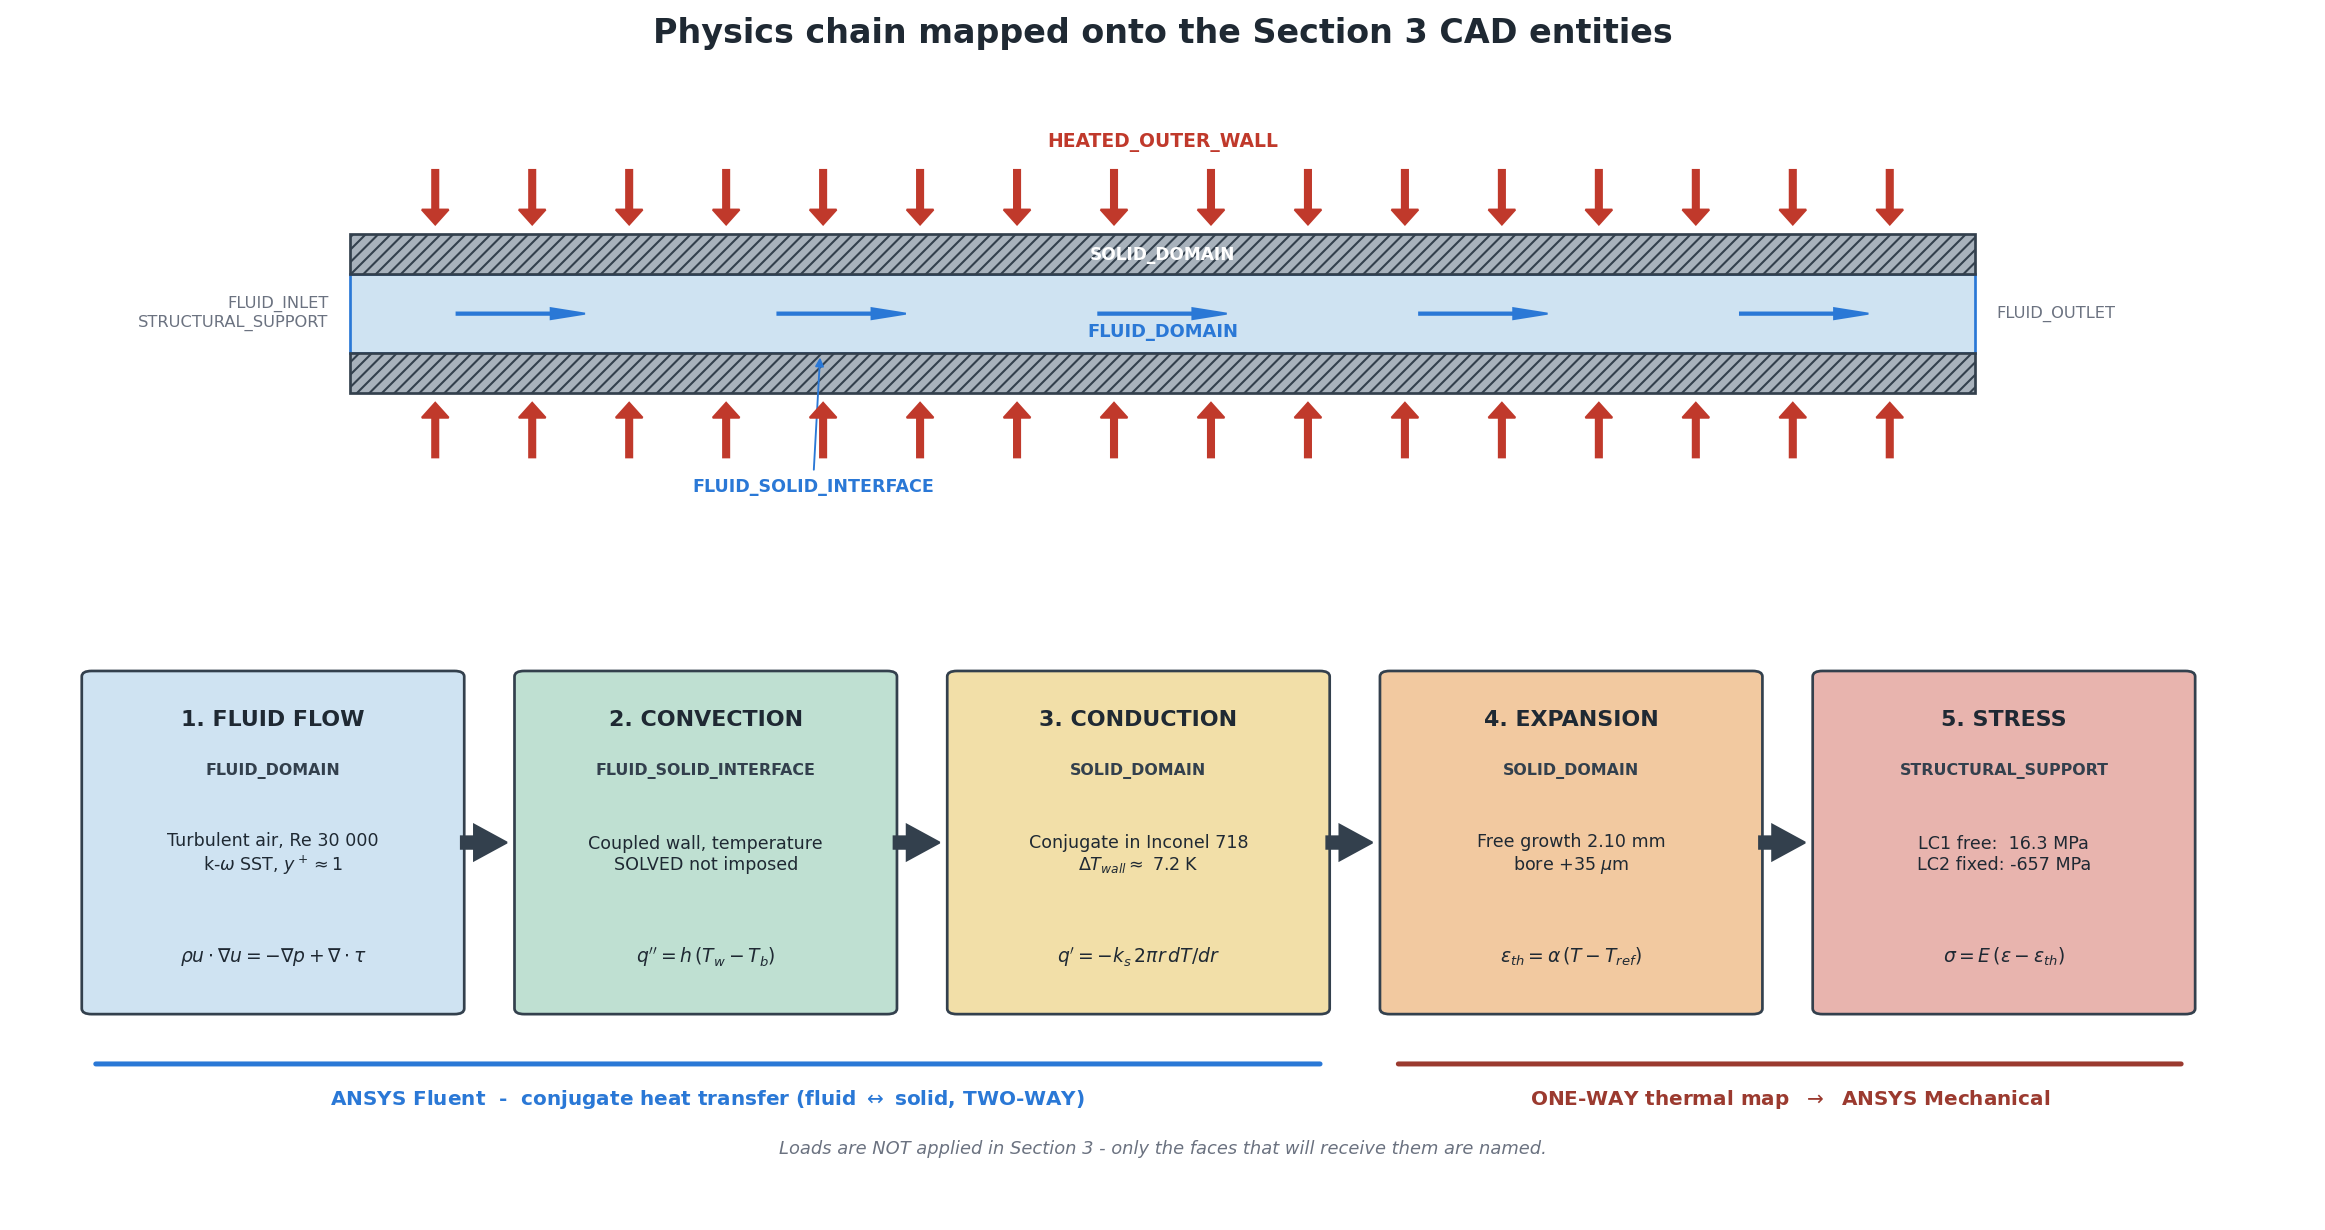
\includegraphics[width=0.80\linewidth]{PHYSICS_SCHEMATIC.png}
\caption[Physics chain mapped onto the CAD entities]{Physics chain mapped onto the CAD entities: flow, convection, conduction, expansion and stress. The values printed in the five
process boxes are Section 2 analytical estimates, not final results.}
\label{fig:physics}
\src{Source: \texttt{03\_CAD\_Geometry/Drawings/PHYSICS\_SCHEMATIC.png} (Section 3).}
\end{figure}

\section{Structural Load Path}
The wall temperature rises from the inlet to the outlet by more than 100~K and exceeds the 300~K stress-free reference everywhere. In free
expansion (LC1) the duct lengthens and only the non-uniform temperature distribution creates stress. When both end faces are held axially
(LC2), the axial growth is prevented; the end supports then react an axial compressive force $N$ equal to the integrated restrained thermal
strain times the axial stiffness of the section. This force is the column load that governs the buckling analysis of Chapter~\ref{ch:buckling}.

\section{Baseline Operating Condition}
The baseline operating point P00 is summarised in Table~\ref{tab:operating}. The inlet Reynolds number of about 30,000 places the flow well
inside the turbulent regime; the bulk temperature rise of about 69~K reduces the Reynolds number to 25,545 at the outlet.

%% generated by gen_tables.py - RE-ANALYSIS 2026
\begin{table}[htbp]
\centering
\small
\caption{Baseline operating condition P00 (selected inputs)}
\label{tab:operating}
\begin{tabular}{>{\raggedright\arraybackslash}p{0.45\linewidth}rl>{\raggedright\arraybackslash}p{0.25\linewidth}}
\toprule
Quantity & Value & Unit & Status \\
\midrule
Fluid & air & -- & selected \\
Inlet temperature $T_{in}$ & 300 & K & selected \\
Inlet velocity $V_{in}$ (uniform) & 23.5 & m/s & selected \\
Inlet turbulence intensity & 4.411 & \% & assumed (A-020b) \\
Outlet static pressure (gauge) & 0 & Pa & selected \\
Operating pressure $p_{op}$ & 101,325 & Pa & selected \\
Outer-wall heat flux $q''$ (uniform) & 8000 & W/m$^2$ & selected \\
Equivalent bore flux $q''D_o/D_i$ & 16,000 & W/m$^2$ & calculated \\
End faces & adiabatic & -- & assumed (A-011) \\
Inlet Reynolds number (CFD) & 29,958 & -- & simulated \\
\bottomrule
\end{tabular}
\par\smallskip\parbox{\linewidth}{\footnotesize\raggedright Source: \texttt{MASTER\_PROJECT\_DATA.csv} rows M002--M006 and M034; \texttt{baseline\_parameters.json}.}
\end{table}


% ===================================================================== Chapter 3
\chapter{Theoretical Foundation}\label{ch:theory}
This chapter collects the relations used by the analytical baseline and for interpreting the simulations. They are standard published
theory; what is specific to this study is the choice of relations and the parameters fed into them. SI units are used throughout.

\section{Internal Flow}
Fluent solves the steady Reynolds-averaged conservation equations for mass, momentum and energy in the air, closed with the $k$--$\omega$
SST model \cite{menter1994}, and the steady heat-conduction equation $\nabla\cdot(k_s\nabla T) = 0$ in the solid. The two regions are
coupled by continuity of temperature and heat flux at the interface. The air is treated as an incompressible ideal gas,
\begin{equation}
\rho = \frac{p_{op}}{R\,T}, \qquad R = 287.058~\text{J/(kg\,K)},\; p_{op} = 101{,}325~\text{Pa},
\label{eq:idealgas}
\end{equation}
so that density follows temperature but not the local pressure; this is admissible because the pressure drop is 0.43\,\% of $p_{op}$.

\section{Reynolds Number}
With mass flux $G = \dot m/A_c$, which stays constant along the duct although the density falls,
\begin{equation}
Re = \frac{\rho V D_h}{\mu} = \frac{G D_h}{\mu}, \qquad D_h = \frac{4A_c}{P_w} = D_i ,
\label{eq:re}
\end{equation}
where $V$ is the mean velocity [m/s], $\mu$ the dynamic viscosity [Pa\,s] and $P_w$ the wetted perimeter [m]. Flow in a circular duct is
turbulent for $Re > 4000$.

\section{Pressure Loss}
The static pressure drop of the heated duct consists of wall friction, thermal acceleration of the expanding gas and the extra loss of the
developing entry region:
\begin{align}
\Delta p_{fr} &= f\,\frac{L}{D_h}\,\frac{\rho V^2}{2}, \label{eq:darcy}\\
f &= \left(0.790\ln Re - 1.64\right)^{-2} \quad (3\times10^3 < Re < 5\times10^6), \label{eq:petukhov}\\
\Delta p_{acc} &= G^2\left(\frac{1}{\rho_{out}} - \frac{1}{\rho_{in}}\right), \qquad \Delta p_{ent} = K_\infty\,\frac{\rho V^2}{2}, \label{eq:acc}
\end{align}
with the Darcy friction factor $f$ from Petukhov \cite{petukhov1970} and the turbulent entry increment $K_\infty \approx 0.09$
\cite{kayslondon}. Entrance and exit losses of a real installation are not part of the CFD domain and are never compared with Fluent.

\section{Turbulent Heat Transfer}
The heat-transfer coefficient $h$ [W/(m$^2$\,K)] is defined by Newton's law of cooling,
\begin{equation}
q''_i = h\,(T_{w,i} - T_b),
\label{eq:newton}
\end{equation}
where $q''_i$ is the heat flux at the bore, $T_{w,i}$ the inner-wall temperature and $T_b$ the local bulk temperature. Because the same
heat passes through a smaller area, the bore flux is $q''_i = q''_o D_o/D_i$ = 16,000~W/m$^2$ for the baseline.

\section{Nusselt Number}
The Nusselt number and the two correlations used are
\begin{align}
Nu &= \frac{h D_h}{k}, \label{eq:nu}\\
Nu_{Gn} &= \frac{(f/8)(Re-1000)Pr}{1 + 12.7\sqrt{f/8}\,\left(Pr^{2/3}-1\right)} \quad (3\times10^3 < Re < 5\times10^6,\; 0.5 < Pr < 2000), \label{eq:gnielinski}\\
Nu_{DB} &= 0.023\,Re^{0.8}Pr^{0.4}, \label{eq:db}
\end{align}
from Gnielinski \cite{gnielinski1976} and Dittus and Boelter \cite{dittus1930}. Both are constant-property correlations; for a gas heated
with a large wall-to-bulk temperature difference the analytical model applies the property-ratio correction \cite{kayscrawford}
\begin{equation}
Nu = Nu_{cp}\left(\frac{T_b}{T_w}\right)^{n}, \qquad n \approx 0.5 .
\label{eq:propcorr}
\end{equation}

\section{Convective Heat Transfer}
Equations~\eqref{eq:newton}--\eqref{eq:propcorr} give the film temperature difference $T_{w,i} - T_b = q''_i/h$. In the analytical model this
difference is about 206~K at the exit, far larger than the 7~K through the wall. In the CFD, $h$ follows from the resolved near-wall
temperature gradient; the ratio of the CFD value to Equation~\eqref{eq:propcorr} is itself a result (Chapter~\ref{ch:cfdres}).

\section{Conduction Through Solid Wall}
For steady radial conduction without generation, with heat per unit length $q'$ [W/m],
\begin{align}
T(r) &= T(r_i) + \frac{q'}{2\pi k_s}\ln\frac{r}{r_i}, \qquad \Delta T_{wall} = \frac{q'}{2\pi k_s}\ln\frac{r_o}{r_i}, \label{eq:fourier}\\
R_{cond} &= \frac{\ln(r_o/r_i)}{2\pi k_s L}, \qquad R_{conv} = \frac{1}{h A_i}. \label{eq:resist}
\end{align}
The temperature rises logarithmically towards the heated outer surface. The resistance ratio $R_{cond}/R_{conv}$ decides whether the metal
or the air film controls the wall temperature.

\section{Energy Balance}
The imposed heat is carried away by the air:
\begin{equation}
Q = q''_o\,A_o = \dot m\,c_p\,(T_{out} - T_{in}), \qquad \frac{dT_b}{dz} = \frac{q''_i\,P_w}{\dot m\,c_p} .
\label{eq:energy}
\end{equation}
At constant flux the bulk temperature rises linearly along the duct. The outlet bulk temperature depends only on $Q$, $\dot m$ and $c_p$,
not on $h$, which makes Equation~\eqref{eq:energy} the strongest single check of a CFD solution.

\section{Thermal Expansion}
The free thermal strain and the resulting free axial growth are
\begin{equation}
\varepsilon_{th} = \alpha_s(T)\,\left(T - T_{ref}\right), \qquad \Delta L = \int_0^L \bar\varepsilon_{th}(z)\,dz ,
\label{eq:thermalstrain}
\end{equation}
where $\alpha_s$ is the secant (mean) expansion coefficient referred to $T_{ref}$ = 300~K and $\bar\varepsilon_{th}$ the section-mean
strain. Thermoelastic Hooke's law adds $\varepsilon_{th}$ to the mechanical strain:
$\varepsilon_{ij} = \left[(1+\nu)\sigma_{ij} - \nu\sigma_{kk}\delta_{ij}\right]/E + \varepsilon_{th}\,\delta_{ij}$.

\section{Thermal Stress}
Stress appears only where thermal strain is prevented, by external restraint or by neighbouring material at a different temperature. For a
fully restrained member with a section-mean temperature rise $\Delta\bar T$,
\begin{equation}
\bar\sigma_z = -E\,\alpha_s\,\Delta\bar T, \qquad N = \int_A E\,\alpha_s\,\Delta T\,dA .
\label{eq:restrained}
\end{equation}
For a long cylinder with free ends and a logarithmic radial temperature distribution, the hoop stress at the bore is
\cite{timoshenko}
\begin{equation}
\sigma_\theta(a) = \frac{\alpha E\,T_a}{2(1-\nu)\ln(b/a)}\left[1 - \frac{2b^2}{b^2-a^2}\ln\frac{b}{a}\right], \qquad T_a = T_i - T_o ,
\label{eq:timoshenko}
\end{equation}
with $a = r_i$ and $b = r_o$. Stresses are assessed with the von Mises equivalent stress
\begin{equation}
\sigma_{vM} = \sqrt{\tfrac12\left[(\sigma_r-\sigma_\theta)^2 + (\sigma_\theta-\sigma_z)^2 + (\sigma_z-\sigma_r)^2\right]}
\label{eq:vm}
\end{equation}
against the yield strength at the local temperature, which defines the yield utilisation $\sigma_{vM}/S_y(T)$ and the first-yield load
factor $S_y(T)/\sigma_{vM}$.

\section{Buckling Fundamentals}
A straight column under axial compression $N$ has the elastic critical load
\begin{equation}
P_E = \frac{\pi^2 E I}{(K L)^2}, \qquad r = \sqrt{I/A},
\label{eq:euler}
\end{equation}
where $K$ is the effective-length factor set by the end conditions: 1.0 for a guided column whose ends can translate but not rotate,
0.699 for fixed--pinned and 0.5 for fixed--fixed. For a stocky section the shear deformation reduces the load,
$P = P_E/\left(1 + P_E/(k G A)\right)$ with Cowper's shear coefficient $k$ \cite{cowper1966}. When the slenderness $KL/r$ is below
$C_c = \sqrt{2\pi^2E/S_y}$ the column is intermediate and the conventional Johnson parabola
$\sigma_{cr} = S_y - \left(S_y^2/4\pi^2E\right)(KL/r)^2$ gives an inelastic estimate. Because the axial force here is thermal and
displacement-controlled, the buckling load factor is expressed as $P_{cr}/N$.

\section{Linear Eigenvalue Buckling}
ANSYS computes the load factor $\lambda$ that multiplies the pre-stress state of LC2 (the full thermal load) from the eigenvalue problem
\begin{equation}
\left([K] + \lambda\,[K_\sigma]\right)\{\phi\} = \{0\}, \qquad P_{cr} = \lambda_1\,N ,
\label{eq:eigen}
\end{equation}
where $[K]$ is the elastic stiffness matrix, $[K_\sigma]$ the stress-stiffness matrix of the LC2 solution and $\{\phi\}$ the mode shape. The
first eigenvalue $\lambda_1$ is the bifurcation load factor of a perfectly straight, linear-elastic structure with idealised supports. It
contains no imperfection, no plasticity and no large-deflection effect. It is therefore a linear stability indicator for an idealised
model, \textbf{not} a guaranteed real-world collapse load and not a factor of safety; an imperfect real duct deflects laterally before
$\lambda_1$ is reached and its capacity is lower by an amount that only a nonlinear analysis can quantify.

% ===================================================================== Chapter 4
\chapter{Engineering Parameters and Materials}\label{ch:params}

\section{Geometry Parameters}
The geometry of Table~\ref{tab:geometry} was chosen by decision D-008: a bore of 20~mm with $L/D_i$ = 30 gives a turbulent flow that
develops over the first 18 diameters; $D_o/D_i$ = 2 gives a wall whose conduction resistance is small but measurable. For the thickness
study the outer diameter is changed to 36 and 44~mm with the bore unchanged.

\section{Fluid Properties}
Air is modelled with temperature-dependent specific heat, viscosity and conductivity from Incropera and DeWitt, Table A.4 \cite{incropera}
(Table~\ref{tab:air}). A cross-check against a second table \cite{cengel} showed about 3\,\% spread in $k$ and $Pr$, which partly cancel to
less than 2\,\% in $h$. Density is not read from the table, whose values refer to 100~kPa; it is computed from Equation~\eqref{eq:idealgas}
at 101,325~Pa. The CFD inlet density implied by the solved mass flow agrees with the analytical value to 0.006\,\%.

%% generated by gen_tables.py - RE-ANALYSIS 2026
\begin{table}[htbp]
\centering
\small
\caption{Air properties used by the analytical model (at the inlet and outlet bulk temperatures)}
\label{tab:air}
\begin{tabular}{lrrl}
\toprule
Property & 300 K & 368.9 K & Unit \\
\midrule
Density $\rho = p_{op}/(RT)$ & 1.1766 & 0.9569 & kg/m$^3$ \\
Specific heat $c_p$ & 1007 & 1011 & J/(kg\,K) \\
Dynamic viscosity $\mu$ & $1.846\times10^{-5}$ & $2.176\times10^{-5}$ & Pa\,s \\
Thermal conductivity $k$ & 0.02624 & 0.03123 & W/(m\,K) \\
Prandtl number $Pr$ & 0.707 & 0.696 & -- \\
\bottomrule
\end{tabular}
\par\smallskip\parbox{\linewidth}{\footnotesize\raggedright Source: \texttt{02\_Engineering\_Calculations/MATERIAL\_PROPERTIES.md}; $c_p$, $\mu$, $k$, $Pr$ from Incropera et al.\ Table A.4 \cite{incropera}; density computed from the ideal-gas law at 101,325~Pa with $R = 287.058$~J/(kg\,K) because tabulated densities refer to 100~kPa. In Fluent, $c_p$, $\mu$ and $k$ are piecewise-linear over 8 points between 250 and 600~K.}
\end{table}


\section{Inconel 718 Properties}
The solid is age-hardened Inconel 718. Temperature-dependent elastic modulus, conductivity, specific heat and proof strength are taken from
the VDM data sheet \cite{vdm718}; the mean thermal expansion coefficient and density from Special Metals data \cite{htm718}
(Table~\ref{tab:inconel}). Poisson's ratio appears in neither data sheet and is an assumption (0.294, literature range 0.284--0.294). The
data are generic datasheet values, not lot-specific properties.

%% generated by gen_tables.py - RE-ANALYSIS 2026
\begin{table}[htbp]
\centering
\small
\caption{Inconel 718 (age-hardened) properties as a function of temperature}
\label{tab:inconel}
\begin{tabular}{lrrrrr}
\toprule
Property & 20\,\textdegree C & 100\,\textdegree C & 200\,\textdegree C & 300\,\textdegree C & 400\,\textdegree C \\
\midrule
Young's modulus $E$ [GPa] & 204 & 199 & 193 & 187 & 180 \\
Thermal conductivity $k_s$ [W/(m\,K)] & 11.5 & 12.1 & 13.5 & 15.2 & 17.1 \\
Specific heat $c_{p,s}$ [J/(kg\,K)] & 460 & 458 & 468 & 485 & 501 \\
0.2\,\% proof strength $S_y$ [MPa] & 1030 & 1060 & 1040 & 1020 & 1000 \\
\midrule
\multicolumn{6}{@{}l}{Mean CTE from 21\,\textdegree C: 12.8 / 13.3 / 13.9 / 14.2 / 14.8 $\times10^{-6}$/K for means to 93 / 204 / 316 / 427 / 538\,\textdegree C} \\
\multicolumn{6}{@{}l}{Density $\rho_s$ = 8190 kg/m$^3$ (constant); Poisson's ratio $\nu$ = 0.294 [ASSUMED], literature range 0.284--0.294} \\
\bottomrule
\end{tabular}
\par\smallskip\parbox{\linewidth}{\footnotesize\raggedright Sources: VDM Alloy 718 Data Sheet No.~4127 \cite{vdm718} ($E$, $k_s$, $c_{p,s}$, $S_y$); High Temp Metals / Special Metals technical data \cite{htm718} (mean CTE, density). Poisson's ratio is in neither datasheet and is an assumption (A-021). $S_y$ values are typical, not minimum-guaranteed (A-022). In Mechanical the secant CTE is re-referenced from its 70\,\textdegree F datum to $T_{ref} = 300$~K (MPAMOD).}
\end{table}


\section{Temperature-Dependent Properties}
Across the solved temperature range the conductivity of Inconel varies by about 32\,\% and the elastic modulus by about 8\,\%, so constant
properties would change the answer. Fluent uses piecewise-linear $k_s(T)$ and $c_{p,s}(T)$; Mechanical uses $E(T)$ and the secant
$\alpha(T)$, re-referenced from the 70\,\textdegree F datum of the data to $T_{ref}$ = 300~K. The yield strength $S_y(T)$ is used only for
assessment and is interpolated at each node's own temperature. The analytical baseline used single values at the mean temperature
($E$ = 188.1~GPa, $\alpha$ = $13.72\times10^{-6}$/K, $S_y$ = 1023.7~MPa at 281.6\,\textdegree C).

\section{Boundary Conditions}
The CFD boundary conditions are listed in Table~\ref{tab:bc}. The heat flux enters only through \texttt{heated\_outer\_wall}; the interface
temperature is solved, never imposed.

%% generated by gen_tables.py - RE-ANALYSIS 2026
\begin{table}[htbp]
\centering
\small
\caption{CFD boundary conditions (read back from Fluent and verified)}
\label{tab:bc}
\begin{tabular}{>{\raggedright\arraybackslash}p{0.30\linewidth}>{\raggedright\arraybackslash}p{0.22\linewidth}>{\raggedright\arraybackslash}p{0.38\linewidth}}
\toprule
Zone & Type & Value \\
\midrule
\texttt{fluid\_inlet} & velocity inlet & 23.5 m/s normal; 300 K; $I = 4.411$\,\%, $D_h = 0.020$~m \\
\texttt{fluid\_outlet} & pressure outlet & 0 Pa gauge; backflow 300 K; reverse flow prevented \\
\texttt{fluid\_solid\_interface} (+ shadow) & wall, coupled & no-slip; temperature and heat flux solved, never imposed \\
\texttt{heated\_outer\_wall} & wall, heat flux & 8000 W/m$^2$ (the only heat input) \\
\texttt{solid\_inlet\_end}, \texttt{solid\_outlet\_end} & wall, heat flux & 0 W/m$^2$ (adiabatic) \\
\bottomrule
\end{tabular}
\par\smallskip\parbox{\linewidth}{\footnotesize\raggedright Source: \texttt{06\_Fluent\_CFD/FLUENT\_SETUP\_NOTES.md} \S8. A heat-path audit confirmed that the flux is applied exactly once.}
\end{table}


\section{Structural Constraints}
Table~\ref{tab:supports} defines the structural load cases and support scenarios. LC1 is statically determinate, so the duct can expand
freely and any reaction is numerical noise. LC2 holds both complete end faces axially; the three mid-span hoop nodes only remove the rigid-body
rotation. Under LC2 the end faces stay plane and perpendicular to the axis, but the ends are free to translate sideways: in buckling terms
this is a guided (sway) column with $K = 1$. S2 and S3 add lateral restraint at one or both ends. None of the three is a model of a real
flange, whose stiffness is undefined.

%% generated by gen_tables.py - RE-ANALYSIS 2026
\begin{table}[htbp]
\centering
\small
\caption{Structural load cases and support scenarios (idealised boundary conditions)}
\label{tab:supports}
\begin{tabular}{>{\raggedright\arraybackslash}p{0.20\linewidth}>{\raggedright\arraybackslash}p{0.52\linewidth}>{\raggedright\arraybackslash}p{0.18\linewidth}}
\toprule
Case & Constraint definition & Role \\
\midrule
LC1 free expansion & 3 outer-ring nodes on the inlet face ($\theta$ = 0/120/240\textdegree), $U_\theta = U_z = 0$ in the duct cylindrical system; statically determinate & gradient stress only \\
LC2 = S1 & $U_z = 0$ on both complete end faces; $U_\theta = 0$ at 3 mid-span outer nodes; radial free; ends free to sway, end rotation held (guided column, $K = 1$) & official baseline \\
S2 & $U_z = U_\theta = 0$ on every node of both end faces (clamped--clamped, $K = 0.5$) & sensitivity \\
S3 & inlet face $U_z = U_\theta = 0$ (clamped); outlet on a deformable remote point on the axis, $U = 0$, rotations free (pinned, $K = 0.699$) & sensitivity \\
\bottomrule
\end{tabular}
\par\smallskip\parbox{\linewidth}{\footnotesize\raggedright Source: \texttt{MASTER\_PROJECT\_DATA.csv} rows M019--M022. None of these represents a defined real flange; the real end restraint is undefined (open task T-034).}
\end{table}


\section{Assumptions}
The principal assumptions and their final status after all simulations are listed in Table~\ref{tab:assumptions}. Several Section 1
assumptions were superseded by the solved models (for example constant material properties); the full register of 31 entries with its
evidence is kept in \texttt{MASTER\_ASSUMPTIONS.md}.

%% generated by gen_tables.py - RE-ANALYSIS 2026
\begin{table}[htbp]
\centering
\footnotesize
\caption{Principal modelling assumptions and their final status}
\label{tab:assumptions}
\begin{tabular}{l>{\raggedright\arraybackslash}p{0.42\linewidth}>{\raggedright\arraybackslash}p{0.14\linewidth}>{\raggedright\arraybackslash}p{0.25\linewidth}}
\toprule
ID & Assumption & Status & Evidence \\
\midrule
A-004 & steady state & valid & time-invariant boundary conditions \\
A-005 & incompressible ideal gas & valid & $\Delta p$ 0.43\,\% of $p_{op}$; Mach $\le$ 0.097 \\
A-007 & buoyancy neglected & valid & $Ri = 4.4\times10^{-5}$ \\
A-008 & viscous dissipation neglected & valid & $Br = 1.8\times10^{-3}$ \\
A-009 & one-way thermal $\rightarrow$ structural coupling & valid & flow-area change 0.70\,\% \\
A-010 & uniform outer-wall heat flux & assumed & idealisation \\
A-011 & adiabatic end faces & assumed & idealisation \\
A-012 & linear elastic material & valid for statics & utilisation $\le$ 0.645 in all cases \\
A-014 & hydraulically smooth wall & assumed & not tested \\
A-015 & internal radiation neglected & assumed / open & not tested (T-009) \\
A-016 & stress-free temperature 300 K & valid & TREF in every solver input \\
A-020b & inlet turbulence intensity 4.411\,\% & assumed & influence limited to the first diameters \\
A-021 & Poisson's ratio 0.294 & assumed & in neither datasheet \\
A-022 & $S_y(T)$ typical datasheet values & assumed & not minimum-guaranteed \\
A-024 & idealised supports S1/S2/S3 & assumed / open & real restraint undefined (T-034) \\
A-025 & perfectly straight tube, no imperfection & assumed & linear eigenvalue buckling (T-035) \\
A-026 & linear elastic buckling & assumed & no stress--strain data (T-036) \\
\bottomrule
\end{tabular}
\par\smallskip\parbox{\linewidth}{\footnotesize\raggedright Source: \texttt{11\_Final\_Audit/MASTER\_ASSUMPTIONS.md} \S3 (full register A-001 to A-031).}
\end{table}


\section{Property Validity Ranges}
Table~\ref{tab:validity} compares the ranges of the property data and correlations with the ranges actually reached. Every solved case stayed
inside the air and Inconel property tables at every iteration. The air table ends at 600~K, which set the lower velocity and upper heat-flux
limits of the parametric study: the highest air-side temperature, 583.4~K in case Q03, is 16.6~K below the table end.

%% generated by gen_tables.py - RE-ANALYSIS 2026
\begin{table}[htbp]
\centering
\footnotesize
\caption{Validity ranges of property data and correlations compared with the solved ranges}
\label{tab:validity}
\begin{tabular}{>{\raggedright\arraybackslash}p{0.30\linewidth}>{\raggedright\arraybackslash}p{0.26\linewidth}>{\raggedright\arraybackslash}p{0.34\linewidth}}
\toprule
Data / correlation & Validity range & Range reached in this project \\
\midrule
Air $c_p$, $\mu$, $k$ table & 250--600 K & baseline fluid 300.0--553.4 K; highest air-side temperature 583.4 K (Q03) \\
Inconel $k_s$, $c_{p,s}$ table & 293--673 K & baseline solid 423.97--562.13 K (cell centres); highest 591.13 K (Q03) \\
Inconel $E$, $S_y$ table & 20--400\,\textdegree C & mapped field 150.69--289.41\,\textdegree C; highest 318.0\,\textdegree C (Q03) \\
Petukhov friction factor & $3\times10^3 < Re < 5\times10^6$ & $Re$ = 25,545--32,954 \\
Gnielinski Nusselt number & $3\times10^3 < Re < 5\times10^6$, $0.5 < Pr < 2000$ & inside \\
Dittus--Boelter Nusselt number & $Re > 10^4$, small wall-to-bulk $\Delta T$ & wall-to-bulk $\Delta T$ up to 206 K: outside, used only as an upper reference \\
\bottomrule
\end{tabular}
\par\smallskip\parbox{\linewidth}{\footnotesize\raggedright Sources: \texttt{MATERIAL\_PROPERTIES.md}, \texttt{CFD\_BASELINE\_RESULTS.md} \S8, \texttt{PROJECT\_STATE.md} \S18.5 and \S19.6. No property was extrapolated in any solved case.}
\end{table}


% ===================================================================== Chapter 5
\chapter{CAD and Computational Model}\label{ch:cad}

\section{SpaceClaim Geometry}
The geometry was built in ANSYS SpaceClaim entirely by an IronPython script run in batch mode, so that re-running one file
reproduces it. The solid annulus is sketched as two concentric circles ($R$ = 20 and 10~mm) and extruded 600~mm. SpaceClaim resolves the two
circles into a single annular face, so the bore produces no body of its own; a first build therefore contained only one body. The
fluid body is created by a second sketch and extrusion of the $R$ = 10~mm disc. An assertion on the body count caught the behaviour.

\section{Fluid-Solid Domain Creation}
The model contains two coincident bodies: \texttt{SOLID\_DOMAIN} (4 faces) and \texttt{FLUID\_DOMAIN} (3 faces). The fluid is a real body, not a
void, so that it can be meshed and becomes a Fluent cell zone. \texttt{ShareTopology.FindAndFix} made the $\diameter$20 interface conformal,
which lets Fluent create a coupled wall/wall-shadow pair without interpolation. Figure~\ref{fig:cad} shows renders of the exported geometry.

\begin{figure}[htbp]
\centering
\begin{subfigure}[t]{0.32\linewidth}\centering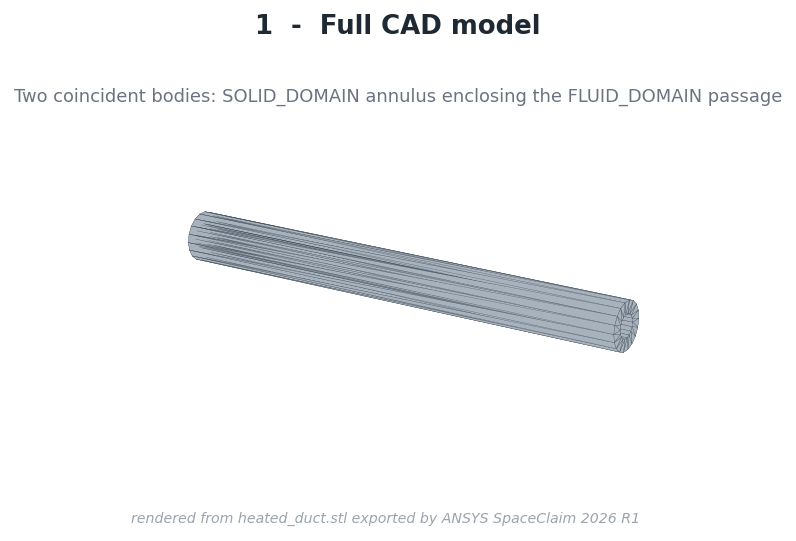
\includegraphics[width=\linewidth]{01_full_cad_model.png}\caption{Full model}\end{subfigure}\hfill
\begin{subfigure}[t]{0.30\linewidth}\centering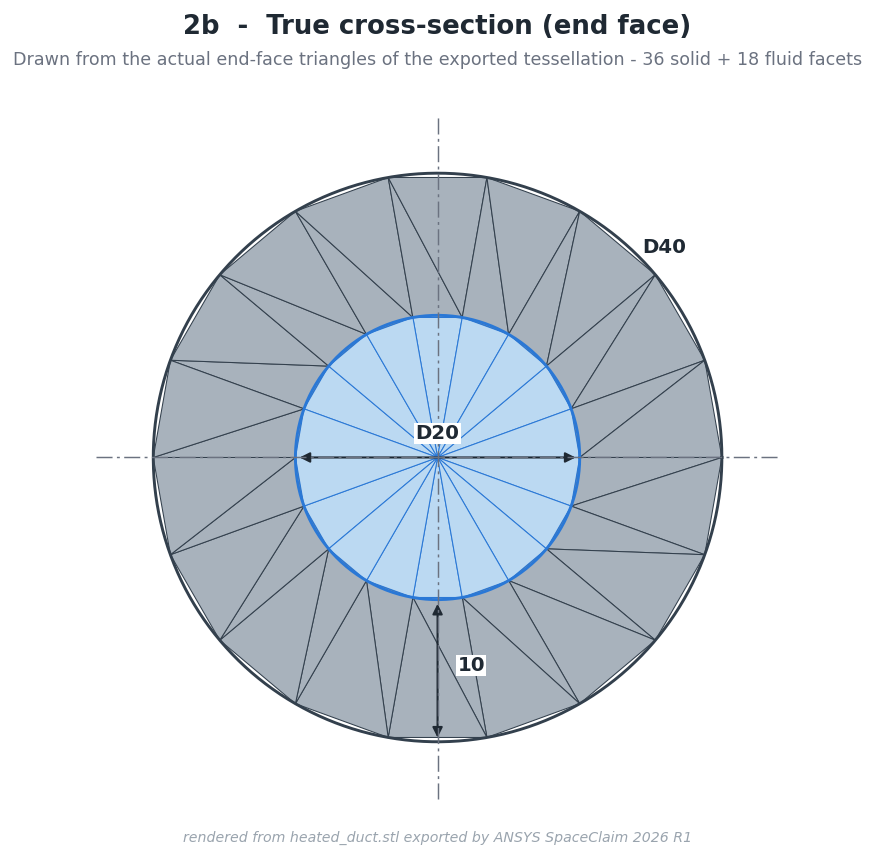
\includegraphics[width=\linewidth]{02b_cross_section_end_on.png}\caption{End-face cross-section}\end{subfigure}\hfill
\begin{subfigure}[t]{0.32\linewidth}\centering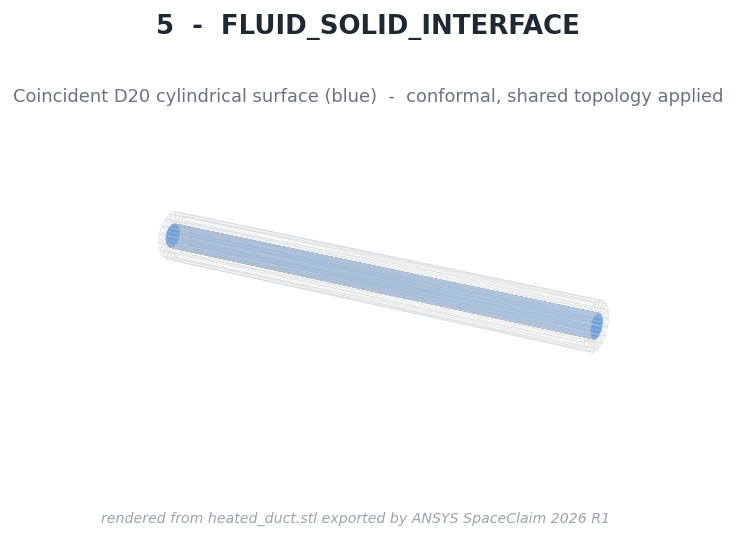
\includegraphics[width=\linewidth]{05_fluid_solid_interface.png}\caption{Fluid--solid interface}\end{subfigure}
\caption[CAD model]{CAD model: solid annulus enclosing the fluid body, and the shared $\diameter$20 interface.}
\label{fig:cad}
\src{\provcad{} The renders use the reference STL tessellation (18 facets per circle), which is why the circles appear polygonal; the meshing source is the native model.}
\end{figure}

\section{Named Selections}
Eleven named selections were created by classifying faces by area and bounding box (Table~\ref{tab:namedsel}). They carry every boundary
condition of the CFD and structural models. The structural support face is deliberately an end face only; restraining the cylindrical wall
would suppress the free growth that LC1 is meant to measure.

%% generated by gen_tables.py - RE-ANALYSIS 2026
\begin{table}[htbp]
\centering
\footnotesize
\caption{Named selections created in SpaceClaim and carried into Fluent and Mechanical}
\label{tab:namedsel}
\begin{tabular}{l>{\raggedright\arraybackslash}p{0.30\linewidth}>{\raggedright\arraybackslash}p{0.32\linewidth}}
\toprule
Name & Entity & Use \\
\midrule
\texttt{FLUID\_DOMAIN} & body: air passage & Fluent fluid cell zone \\
\texttt{SOLID\_DOMAIN} & body: Inconel 718 annulus & Fluent solid zone; Mechanical body \\
\texttt{FLUID\_INLET} & \O{}20 disc at $z = 0$ & velocity inlet \\
\texttt{FLUID\_OUTLET} & \O{}20 disc at $z = 600$ mm & pressure outlet \\
\texttt{FLUID\_WALL} & \O{}20 cylinder, fluid side & near-wall grading, $y^+$ monitoring \\
\texttt{FLUID\_SOLID\_INTERFACE} & both sides of the \O{}20 surface & conjugate coupling \\
\texttt{SOLID\_INNER\_INTERFACE} & \O{}20 cylinder, solid side & conjugate coupling \\
\texttt{HEATED\_OUTER\_WALL} & \O{}40 cylinder & heat flux 8000 W/m$^2$ \\
\texttt{SOLID\_INLET\_END} & annulus at $z = 0$ & adiabatic \\
\texttt{SOLID\_OUTLET\_END} & annulus at $z = 600$ mm & adiabatic \\
\texttt{STRUCTURAL\_SUPPORT} & annulus at $z = 0$ & structural restraint face \\
\bottomrule
\end{tabular}
\par\smallskip\parbox{\linewidth}{\footnotesize\raggedright Source: \texttt{03\_CAD\_Geometry/CAD\_NOTES.md} \S6. All 11 selections survived the transfer to Workbench Meshing without re-creation.}
\end{table}


\section{Geometry Verification}
Every dimension, area and volume of the saved model was compared with its analytical value (Table~\ref{tab:geomver}). All agree to
double-precision round-off (largest relative deviation $1.8\times10^{-14}$\,\%). The model has 7 faces, no open surfaces, no sliver faces and
no defeaturing needs.

%% generated by gen_tables.py - RE-ANALYSIS 2026
\begin{table}[htbp]
\centering
\footnotesize
\caption{Geometry verification: analytical values against the SpaceClaim model}
\label{tab:geomver}
\begin{tabular}{lrrl}
\toprule
Quantity & Analytical & CAD & Relative difference \\
\midrule
Fluid cross-sectional area [mm$^2$] & 314.1592654 & 314.1592654 & $1.8\times10^{-14}$\,\% \\
\texttt{FLUID\_DOMAIN} volume [m$^3$] & $1.884955592\times10^{-4}$ & $1.884955592\times10^{-4}$ & $1.4\times10^{-14}$\,\% \\
\texttt{SOLID\_DOMAIN} volume [m$^3$] & $5.654866776\times10^{-4}$ & $5.654866776\times10^{-4}$ & 0 \\
\texttt{HEATED\_OUTER\_WALL} area [m$^2$] & 0.07539822369 & 0.07539822369 & 0 \\
Interface area, fluid side = solid side [m$^2$] & 0.03769911184 & 0.03769911184 & 0 (identical to 17 digits) \\
Fluid + solid volume [m$^3$] & \multicolumn{3}{l}{$7.539822369\times10^{-4}$ = full \O{}40 $\times$ 600 mm cylinder (no gap, no overlap)} \\
\bottomrule
\end{tabular}
\par\smallskip\parbox{\linewidth}{\footnotesize\raggedright Source: \texttt{03\_CAD\_Geometry/CAD\_NOTES.md} \S5 and \S7; raw values in \texttt{Geometry\_Check/cad\_measurements.json}.}
\end{table}


\section{Volume Verification}
The strongest single check is the volume sum: fluid plus solid volume equals the volume of the full $\diameter$40 $\times$ 600~mm cylinder,
$7.539822369\times10^{-4}$ m$^3$, to machine precision. An overlap would exceed this value and a gap would fall short of it. The interface
areas on the fluid and solid sides are identical to 17 significant digits.

\section{Workbench Architecture}
The Workbench project links a Geometry system (the native SpaceClaim file, shared), a Mesh system and a Fluent system; it was built by a
Workbench journal in batch mode. All eleven named selections transferred automatically. The CFD meshes themselves were generated by a
Python script (Chapter~\ref{ch:mesh}) and written in the Fluent mesh format. For the structural phase, the Workbench project was saved under
a new name and extended with an External Data system (temperature transfer) and Static Structural systems for LC1 and LC2; linear buckling,
the structural mesh study and each parametric case used further save-as copies, so that every earlier project stayed byte-identical.

\section{Model Preparation}
Before any solve the geometry was checked for sweepability: both domains have constant cross-sections over 600~mm, so hexahedral sweeps apply
directly and no tetrahedra are needed. The parametric thickness cases T01 and T03 were built from a parameterised copy of the same script; their
dimensions, areas and volumes also match the analytical values to round-off. Parasolid export was unavailable in the Student installation;
the native file and STEP were used instead.

% ===================================================================== Chapter 6
\chapter{CFD Methodology}\label{ch:cfdmethod}

\section{Fluent Setup}
The CFD model was set up and solved in ANSYS Fluent 2026 R1 \cite{ansysfluent} under the Student licence (4-way parallel). The case was built by a Python/Fluent
journal that writes each setting and reads it back before continuing; the settings of the final solution were read back once more from the
converged case (Table~\ref{tab:solver}).

%% generated by gen_tables.py - RE-ANALYSIS 2026
\begin{table}[htbp]
\centering
\small
\caption{Fluent solver and physical-model settings of the baseline solution}
\label{tab:solver}
\begin{tabular}{>{\raggedright\arraybackslash}p{0.30\linewidth}>{\raggedright\arraybackslash}p{0.60\linewidth}}
\toprule
Setting & Value \\
\midrule
Software & ANSYS Fluent 2026 R1 (Student licence, 4-way parallel) \\
Solver & pressure-based, coupled pressure--velocity, steady, absolute velocity \\
Energy equation & on (fluid and solid) \\
Turbulence model & $k$--$\omega$ SST, blended wall treatment (\texttt{correlation} $\omega$ wall treatment) \\
Gravity / radiation & off / off \\
Air & incompressible ideal gas, $\rho = p_{op}/(RT)$; $c_p$, $\mu$, $k$ piecewise-linear, 250--600 K \\
Inconel 718 & $\rho$ = 8190 kg/m$^3$; $k_s$, $c_{p,s}$ piecewise-linear, 293--673 K \\
Gradient & least-squares cell-based \\
Initialisation & standard: 300 K, $w$ = 23.5 m/s, 0 Pa gauge in the whole domain (cold start) \\
\bottomrule
\end{tabular}
\par\smallskip\parbox{\linewidth}{\footnotesize\raggedright Source: \texttt{06\_Fluent\_CFD/FLUENT\_SETUP\_NOTES.md} \S5--\S10 and \texttt{Baseline/CFD\_BASELINE\_RESULTS.md} \S2.}
\end{table}


\section{Solver Type}
A pressure-based solver with coupled pressure--velocity treatment was used. The maximum local Mach number is 0.097 at the outlet
centreline, so density-based compressible formulations are not required; the coupled algorithm gives robust convergence of the strongly
coupled velocity, temperature and density fields.

\section{Steady-State Formulation}
All boundary conditions are time-invariant and the physical question concerns the operating state, not the start-up transient; the problem
is therefore solved as steady (A-004). A steady solution is also the correct input for a linear static structural analysis.

\section{Energy Equation}
The energy equation is solved in both the fluid and the solid. Viscous dissipation is negligible (Brinkman number $1.8\times10^{-3}$) and
buoyancy is switched off (Richardson number $4.4\times10^{-5}$). The fluid--solid interface is a coupled wall: temperature and heat flux are
continuous and solved as part of the solution.

\section{k-omega SST}
The $k$--$\omega$ SST model \cite{menter1994} was chosen because it can be integrated through the viscous sublayer to the wall without wall
functions. In conjugate heat transfer the wall heat flux sets the solid temperature, which in turn sets the stress; a wall function would
model the quantity of interest instead of resolving it.

\section{Wall Treatment}
Fluent's blended SST wall treatment with the \texttt{correlation} $\omega$ formulation integrates the equations to the wall when the first cell
centre lies inside the viscous sublayer ($y^+ \lesssim 1$). The mesh was designed with a first fluid cell height of 12.2~\textmu m; the
converged solution confirms $y^+ \le$ 0.585 on the whole conjugate wall (Section~\ref{sec:yplus}).

\section{Material Models}
Air is an incompressible ideal gas with piecewise-linear $c_p$, $\mu$ and $k$ (8 points, 250--600~K). Inconel 718 is a new material with
constant density and piecewise-linear $k_s$ and $c_{p,s}$ (5 points, 293--673~K). Fluent's default solid material carried by the mesh file
was replaced explicitly. Temperature-dependent properties make the CFD consistent with the axially marched analytical model, which used the
same table.

\section{Boundary Conditions}
The boundary conditions of Table~\ref{tab:bc} were read back after assignment. A heat-path audit walked every wall and confirmed that the
flux of 8000~W/m$^2$ is applied only on the outer wall; any second non-zero flux would have been flagged as a double heat input. The inlet
turbulence intensity of 4.411\,\% follows the fully developed pipe estimate $I = 0.16\,Re^{-1/8}$ and is an assumption whose influence is
confined to the first few diameters.

\section{Initialization}
The whole domain, fluid and solid, was initialised from the inlet: 300~K, axial velocity 23.5~m/s and 0~Pa gauge pressure. This cold
start corresponds to the state before heating begins. No solution was initialised from another case.

\section{Numerical Schemes}
Gradients use the least-squares cell-based method and pressure is second-order throughout. The solution was advanced in stages
(Table~\ref{tab:stages}): first-order upwind for momentum, $k$, $\omega$ and energy while the flow and then the thermal field develop, followed by
second-order upwind for all equations. Only the second-order solution is used as a result.

%% generated by gen_tables.py - RE-ANALYSIS 2026
\begin{table}[htbp]
\centering
\footnotesize
\caption{Solution staging and discretisation of the baseline run}
\label{tab:stages}
\begin{tabular}{lllp{0.35\linewidth}}
\toprule
Stage & Iterations & Schemes & Purpose \\
\midrule
1 & 1--150 & first-order upwind, energy off & develop velocity and turbulence fields \\
2 & 151--300 & first-order upwind, energy on & bring up the thermal field \\
3 & 301--600 & second-order (pressure, momentum, $k$, $\omega$, energy) & production discretisation; convergence checked every 100 iterations \\
confirm & 601--700 & second-order & confirm that the converged state holds \\
\bottomrule
\end{tabular}
\par\smallskip\parbox{\linewidth}{\footnotesize\raggedright Source: \texttt{CFD\_BASELINE\_RESULTS.md} \S3. Wall clock 12 min 58 s on 4 cores for 700 iterations, including audits and exports.}
\end{table}


\section{Convergence Criteria}
Residuals alone were not accepted as evidence of convergence. The criteria combine residual targets with physical-monitor plateaus over the
last 200 iterations and with the global mass and energy balances (Table~\ref{tab:convcrit}); they were evaluated every 100 iterations of the
second-order stage.

%% generated by gen_tables.py - RE-ANALYSIS 2026
\begin{table}[htbp]
\centering
\footnotesize
\caption{Convergence criteria and final state of the baseline solution (iteration 700)}
\label{tab:convcrit}
\begin{tabular}{lll}
\toprule
Criterion & Target & Achieved \\
\midrule
Continuity residual & $< 10^{-4}$ & $9.0\times10^{-11}$ \\
Momentum residuals & $< 10^{-4}$ & $\le 1.6\times10^{-14}$ \\
$k$ / $\omega$ residuals & $< 10^{-4}$ & $7.2\times10^{-13}$ / $2.0\times10^{-13}$ \\
Energy residual & $< 10^{-6}$ & $1.6\times10^{-14}$ \\
$T_{out}$ drift over the last 200 iterations & $< 0.1$ K & $2.3\times10^{-6}$ K \\
$\Delta p$ relative drift & $< 0.1$\,\% & $6.9\times10^{-8}$\,\% \\
Interface heat-rate relative drift & $< 0.1$\,\% & $3.5\times10^{-7}$\,\% \\
Mass imbalance & $< 0.01$\,\% & $7.0\times10^{-13}$\,\% \\
Energy imbalance & $< 0.5$\,\% & $3.1\times10^{-11}$\,\% \\
\bottomrule
\end{tabular}
\par\smallskip\parbox{\linewidth}{\footnotesize\raggedright Source: \texttt{CFD\_BASELINE\_RESULTS.md} \S3; imbalances also \texttt{MASTER\_PROJECT\_DATA.csv} rows M047--M048 (VERIFIED).}
\end{table}


\section{Engineering Monitors}
Besides the residuals, fourteen physical monitors were recorded every iteration, among them the outlet bulk temperature, the maximum solid,
wetted-wall and outer-wall temperatures, the pressure drop, the heat rate across the interface and the outlet mass flow. The solid and fluid
temperature ranges were checked against the property tables at every iteration to exclude silent extrapolation.

% ===================================================================== Chapter 7
\chapter{Meshing}\label{ch:mesh}

\section{CFD Mesh Strategy}
Three meshes with the same topology and systematically different resolution were built so that discretisation error could be estimated
later (Chapter~\ref{ch:mi}). The mesh is a structured butterfly (O-grid) hexahedral mesh generated by a Python script and written directly in
the Fluent mesh format; ANSYS Meshing holds the geometry and named selections in the Workbench project. Scripting was chosen for three
reasons: conformality of the interface is guaranteed by construction (fluid and solid share one node table); every sizing control is an
explicit number under version control; and all three levels are regenerated byte-for-byte by one command.

\section{Structured Hexahedral Mesh}
The cross-section consists of a super-ellipse core filled by transfinite interpolation, a graded fluid annulus and a graded solid annulus;
the section is extruded over uniform axial slabs (Figure~\ref{fig:meshxs}a). The core is a rounded square rather than a circle so that its
four edges map onto the annulus without a singular point on the axis. All three levels are 100\,\% hexahedra (Table~\ref{tab:meshfam}).

%% generated by gen_tables.py - RE-ANALYSIS 2026
\begin{table}[htbp]
\centering
\footnotesize
\caption{CFD mesh family: sizing controls (same topology on all levels)}
\label{tab:meshfam}
\begin{tabular}{lrrr}
\toprule
Control & Coarse & Medium & Fine \\
\midrule
Core divisions per side $N_C$ & 8 & 12 & 18 \\
Circumferential divisions $N_\theta = 4N_C$ & 32 & 48 & 72 \\
Fluid radial layers & 18 & 24 & 32 \\
Solid radial layers & 7 & 10 & 15 \\
Axial divisions & 60 & 90 & 135 \\
Axial cell length [mm] & 10.000 & 6.667 & 4.444 \\
First fluid cell height [\textmu m] & 12.2 & 12.2 & 12.2 \\
Fluid growth rate & 1.3182 & 1.2091 & 1.1385 \\
Solid first cell at the interface [mm] & 0.5 & 0.5 & 0.5 \\
\bottomrule
\end{tabular}
\par\smallskip\parbox{\linewidth}{\footnotesize\raggedright Source: \texttt{05\_Meshing/MESH\_NOTES.md} \S3--\S4. Linear refinement ratio $r \approx 1.46$ between levels.}
\end{table}


\begin{figure}[htbp]
\centering
\begin{subfigure}[t]{0.40\linewidth}\centering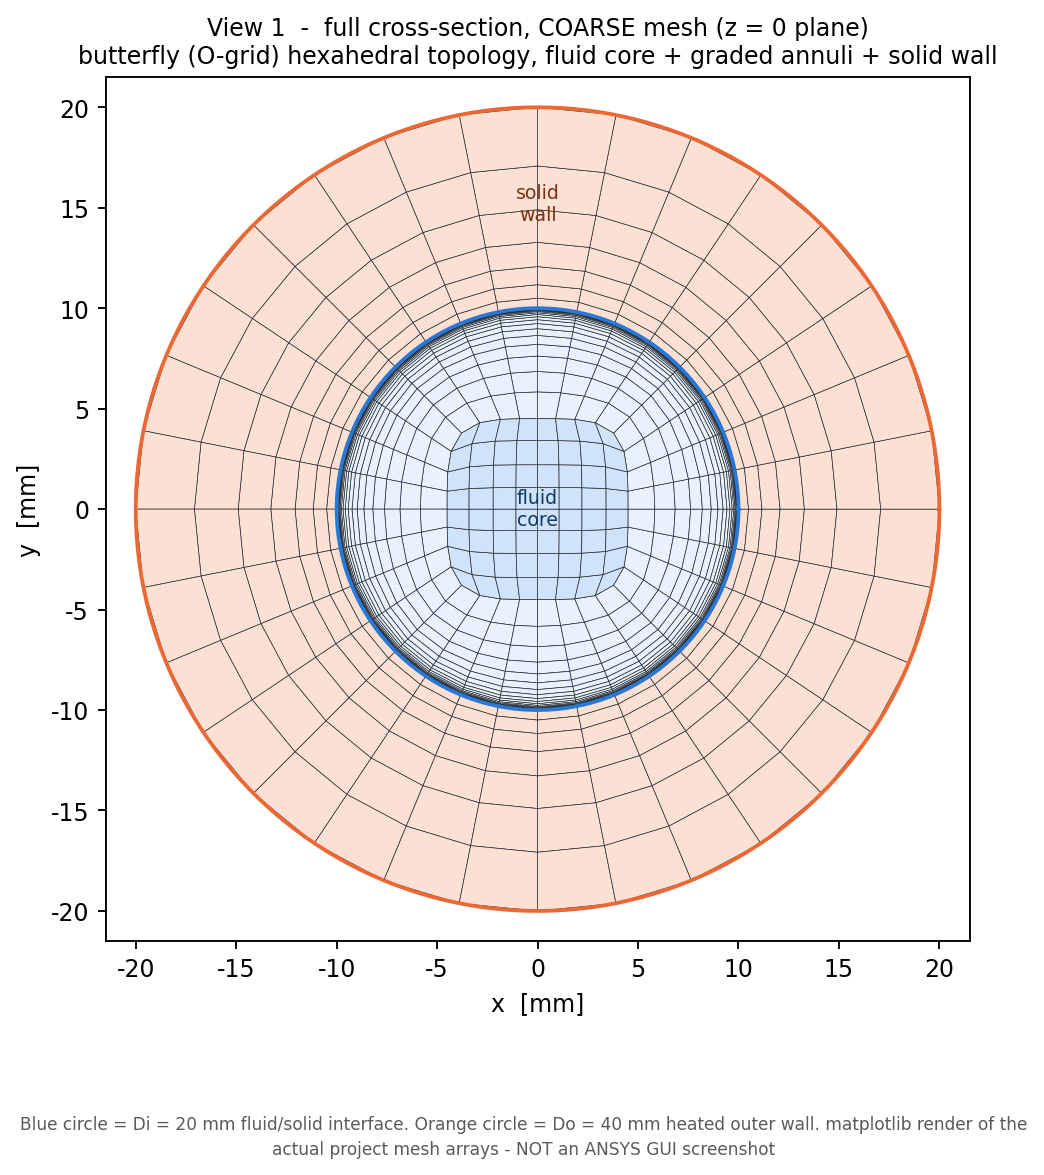
\includegraphics[width=\linewidth]{mesh_01_cross_section_full.png}\caption{Cross-section (coarse level)}\end{subfigure}\hfill
\begin{subfigure}[t]{0.58\linewidth}\centering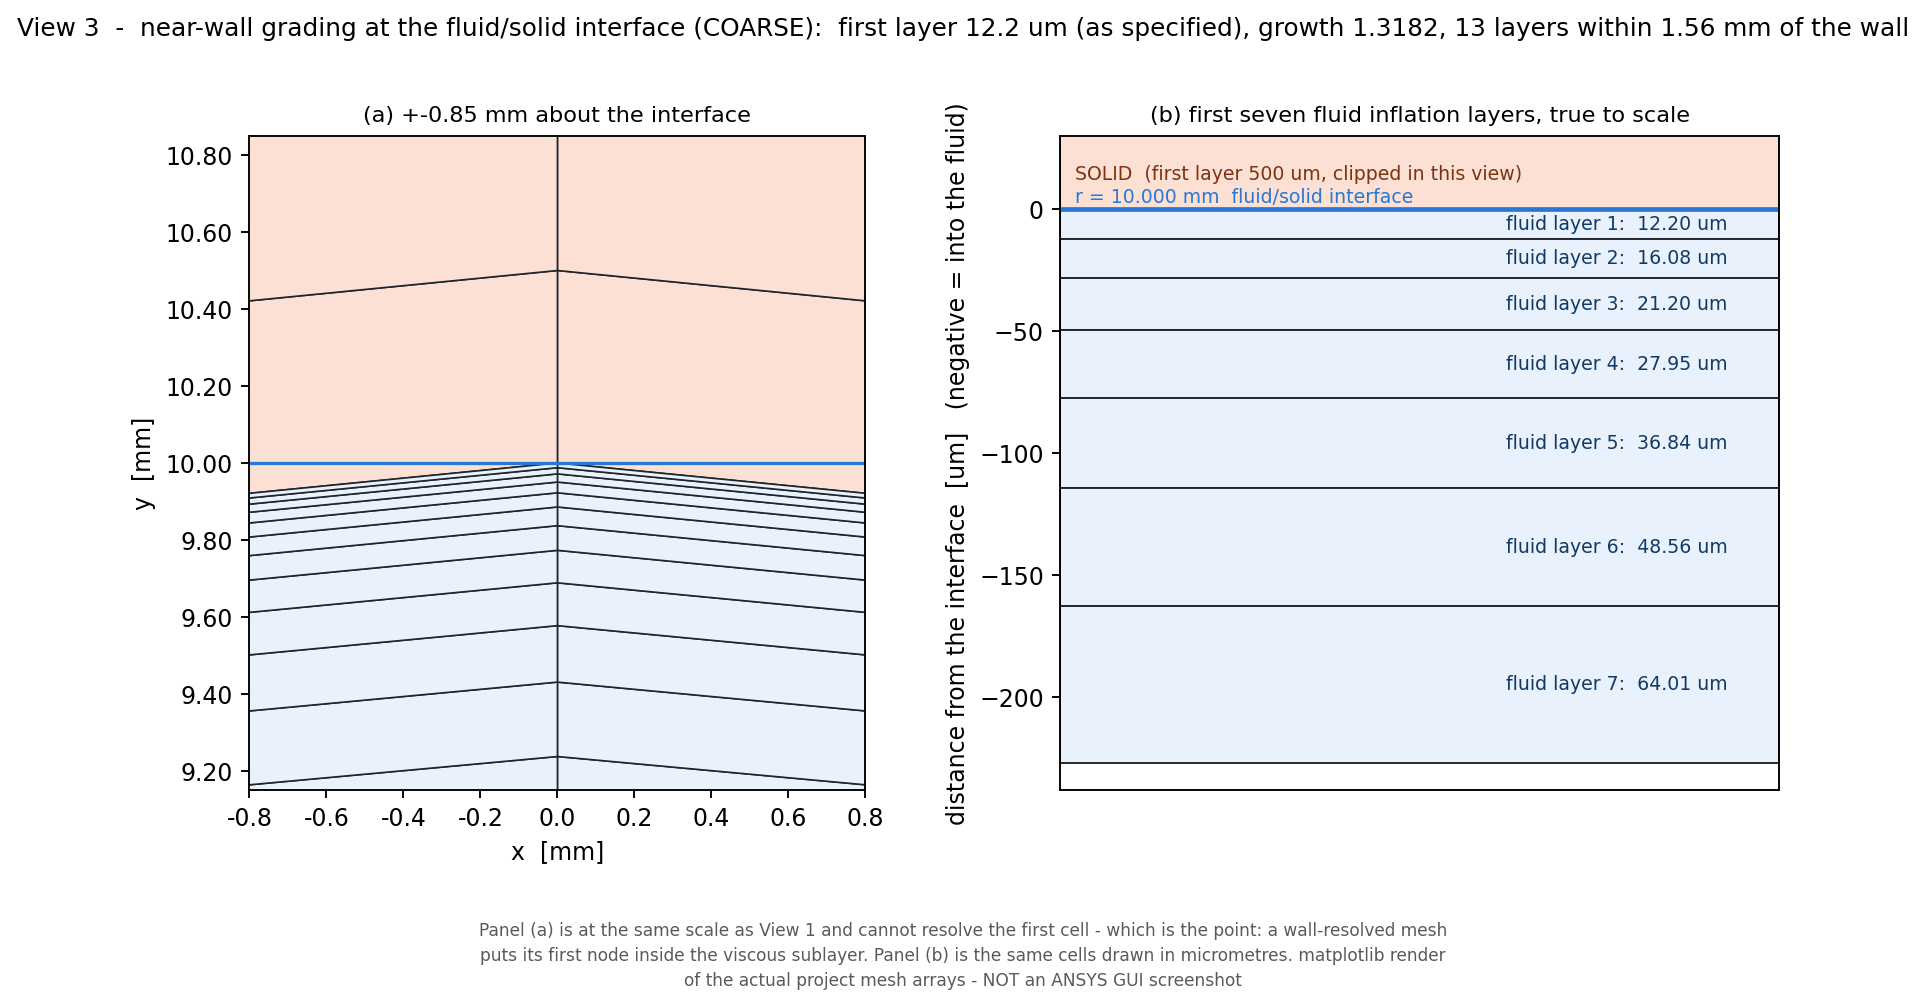
\includegraphics[width=\linewidth]{mesh_03_inflation_near_wall.png}\caption{Near-wall grading at the interface}\end{subfigure}
\caption[Structured O-grid CFD mesh]{Structured O-grid CFD mesh: fluid core, graded fluid annulus and solid wall; the first fluid layers next to the interface are drawn true to scale in (b).}
\label{fig:meshxs}
\src{\provmesh}
\end{figure}

\section{Near-Wall Resolution}
A wall-resolved SST solution requires the first cell centre inside the viscous sublayer. The first-layer height of 12.2~\textmu m was derived
from the Section 2 wall-shear estimate for $y^+ \approx 1$. The converged solution showed that the height holds on the four O-grid axes but
is about 15\,\% smaller at the diagonals (about 10.4~\textmu m), a geometric consequence of the super-ellipse core. The resulting
circumferential $y^+$ pattern is geometric rather than physical (the wall shear varies by only 0.078\,\% around the circumference) and is
harmless because the cells are thinner, not thicker, than designed.

\section{Inflation / First Cell}
The mesh has no separate prism stack; instead the whole fluid annulus is a geometrically graded ring stack solved so that it exactly fills
the annulus from the 12.2~\textmu m first layer. The first-layer height is identical on all three levels, so that the near-wall treatment does
not change with refinement. On the medium mesh, 17 layers lie within 1.56~mm of the wall. The solid starts with a 0.5~mm layer at the interface.

\section{Mesh Quality}
Mesh quality was reported by Fluent (\texttt{mesh/check}, \texttt{mesh/quality}) and reproduced independently by a Python audit to within
$10^{-6}$ relative (Table~\ref{tab:meshq}, Figure~\ref{fig:meshq}). All minima are well above Fluent's orthogonal-quality threshold of 0.1.
The high aspect ratios are intended (thin wall-parallel cells in the near-wall layers). On the fine mesh 540 O-grid corner cells (0.108\,\%)
exceed a skewness of 0.80; the minimum orthogonal quality therefore decreases with refinement, which was located and accepted.

%% generated by gen_tables.py - RE-ANALYSIS 2026
\begin{table}[htbp]
\centering
\footnotesize
\caption{CFD mesh statistics and quality (Fluent \texttt{mesh/check} and \texttt{mesh/quality})}
\label{tab:meshq}
\begin{tabular}{lrrr}
\toprule
Quantity & Coarse & Medium (baseline) & Fine (reference) \\
\midrule
Total cells & 51,840 & 159,840 & 500,580 \\
Fluid / solid cells & 38,400 / 13,440 & 116,640 / 43,200 & 354,780 / 145,800 \\
Conformal interface faces & 1,920 & 4,320 & 9,720 \\
Cell type & 100\,\% hexahedra & 100\,\% hexahedra & 100\,\% hexahedra \\
Minimum orthogonal quality & 0.4482 & 0.4458 & 0.3144 \\
Maximum skewness & 0.6564 & 0.7600 & 0.8364 \\
Maximum aspect ratio & 974.5 & 654.4 & 437.9 \\
Negative-volume cells & 0 & 0 & 0 \\
\bottomrule
\end{tabular}
\par\smallskip\parbox{\linewidth}{\footnotesize\raggedright Source: \texttt{05\_Meshing/MESH\_NOTES.md} \S5--\S6 and \texttt{Mesh\_Quality/MESH\_QUALITY\_TABLE.md}; cell totals \texttt{MASTER\_PROJECT\_DATA.csv} rows M033, M050, M058.}
\end{table}


\section{Coarse / Medium / Fine Meshes}
Refinement is applied in all three directions at once, giving linear refinement ratios of 1.455 and 1.463 between the levels, above the value
of 1.3 recommended for Richardson extrapolation \cite{celik2008}. Figure~\ref{fig:meshref} compares the cross-sections.

\begin{figure}[htbp]
\centering
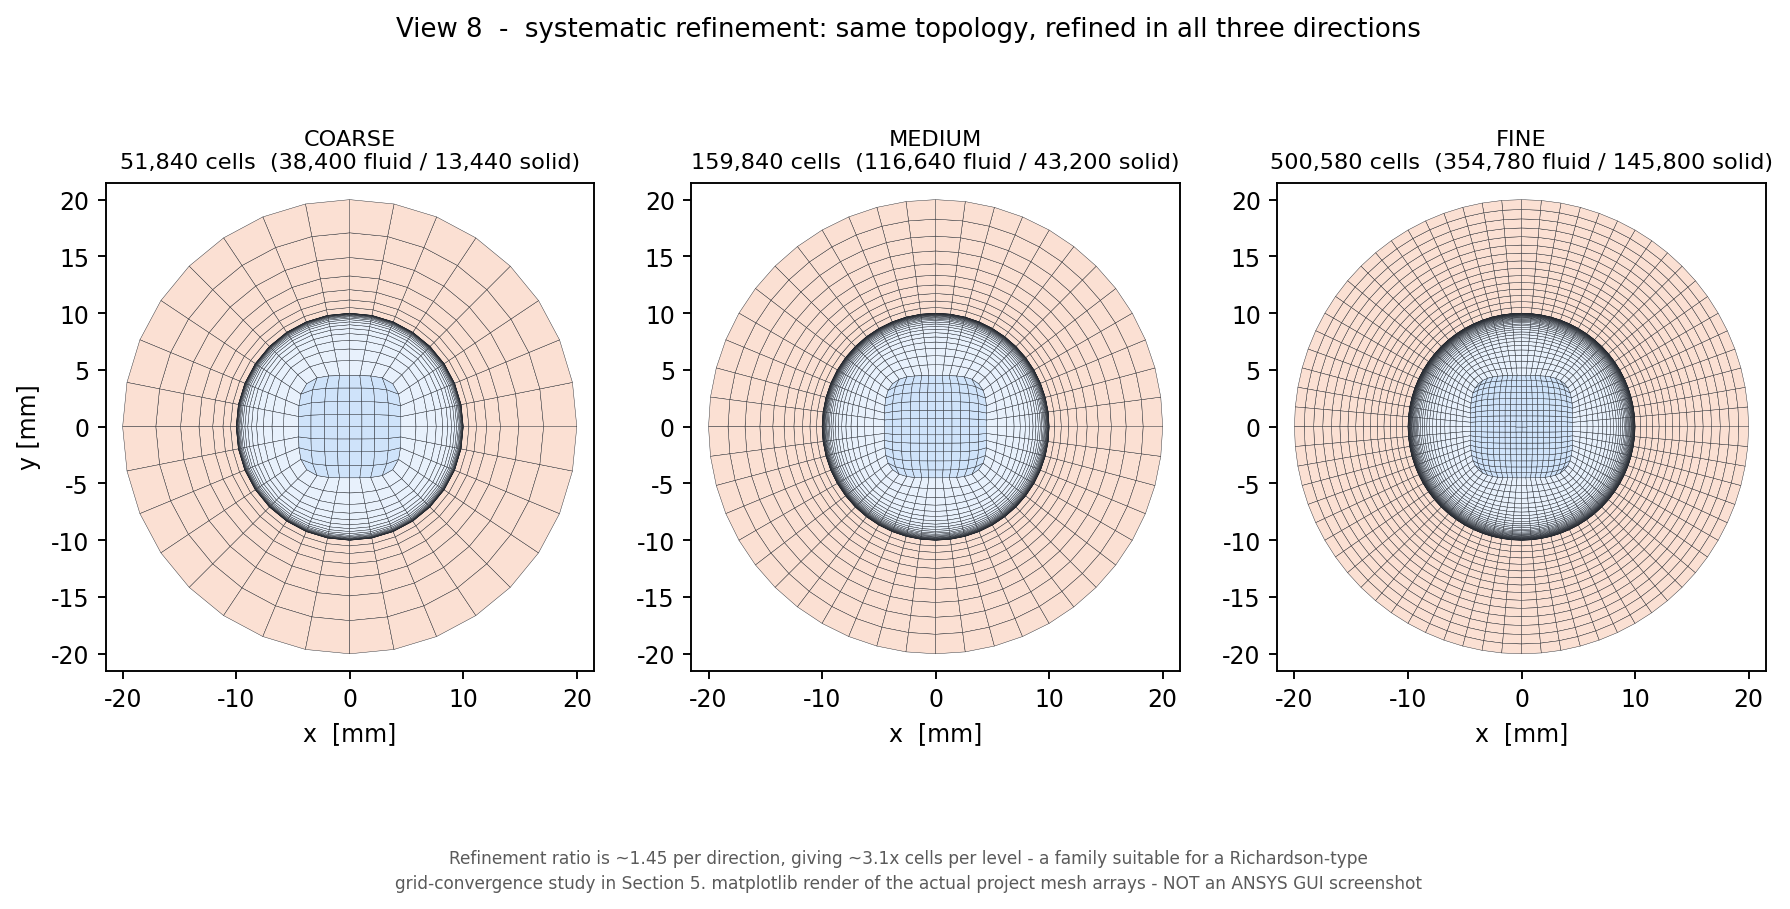
\includegraphics[width=0.80\linewidth]{mesh_08_refinement_comparison.png}
\caption[Systematic refinement of the CFD mesh family]{Systematic refinement of the CFD mesh family: coarse (51,840~cells), medium (159,840~cells, baseline) and fine (500,580~cells).}
\label{fig:meshref}
\src{\provmesh}
\end{figure}

\section{Conformal Fluid-Solid Interface}
The interface has 1,920 / 4,320 / 9,720 faces on the three levels, each with exactly one fluid owner and one solid neighbour; there are no
orphan faces or hanging nodes, and the interface node radius is exact to $1.7\times10^{-18}$ m (Figure~\ref{fig:meshq}a). On reading the mesh,
Fluent creates the coupled \texttt{fluid\_solid\_interface-shadow} pair automatically, confirming the conformal treatment.

\begin{figure}[htbp]
\centering
\begin{subfigure}[t]{0.56\linewidth}\centering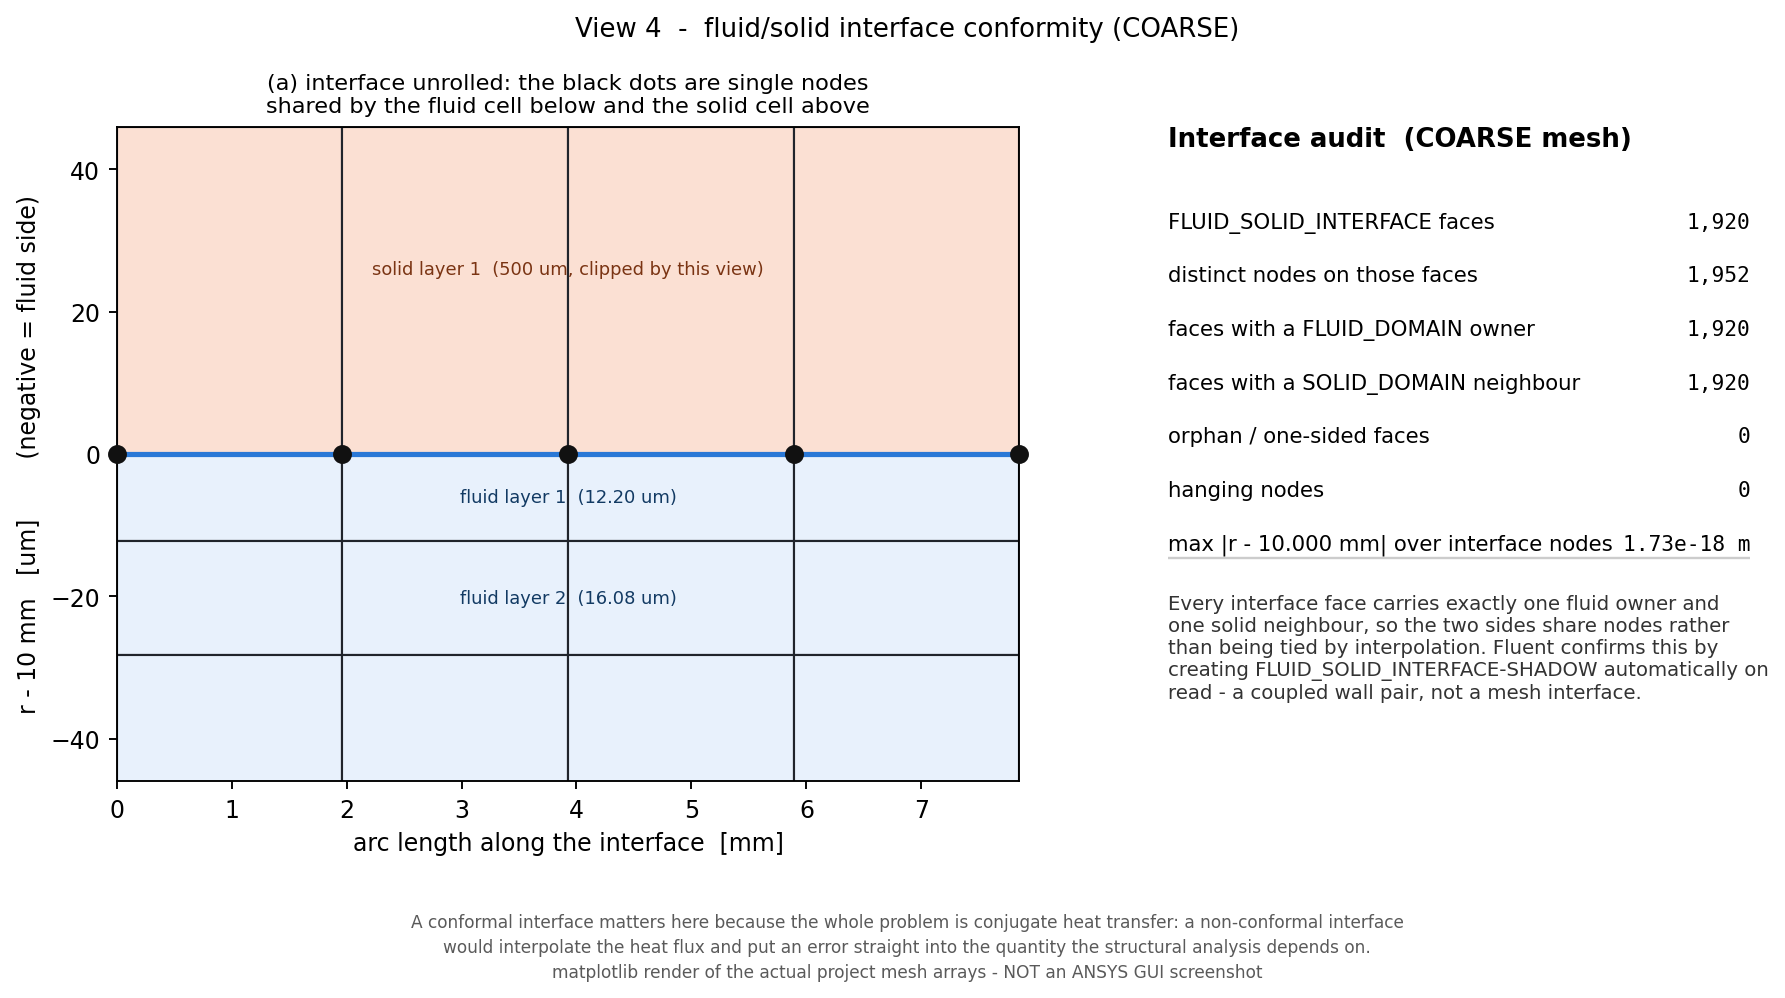
\includegraphics[width=\linewidth]{mesh_04_interface_conformity.png}\caption{Interface conformity audit (coarse)}\end{subfigure}\hfill
\begin{subfigure}[t]{0.42\linewidth}\centering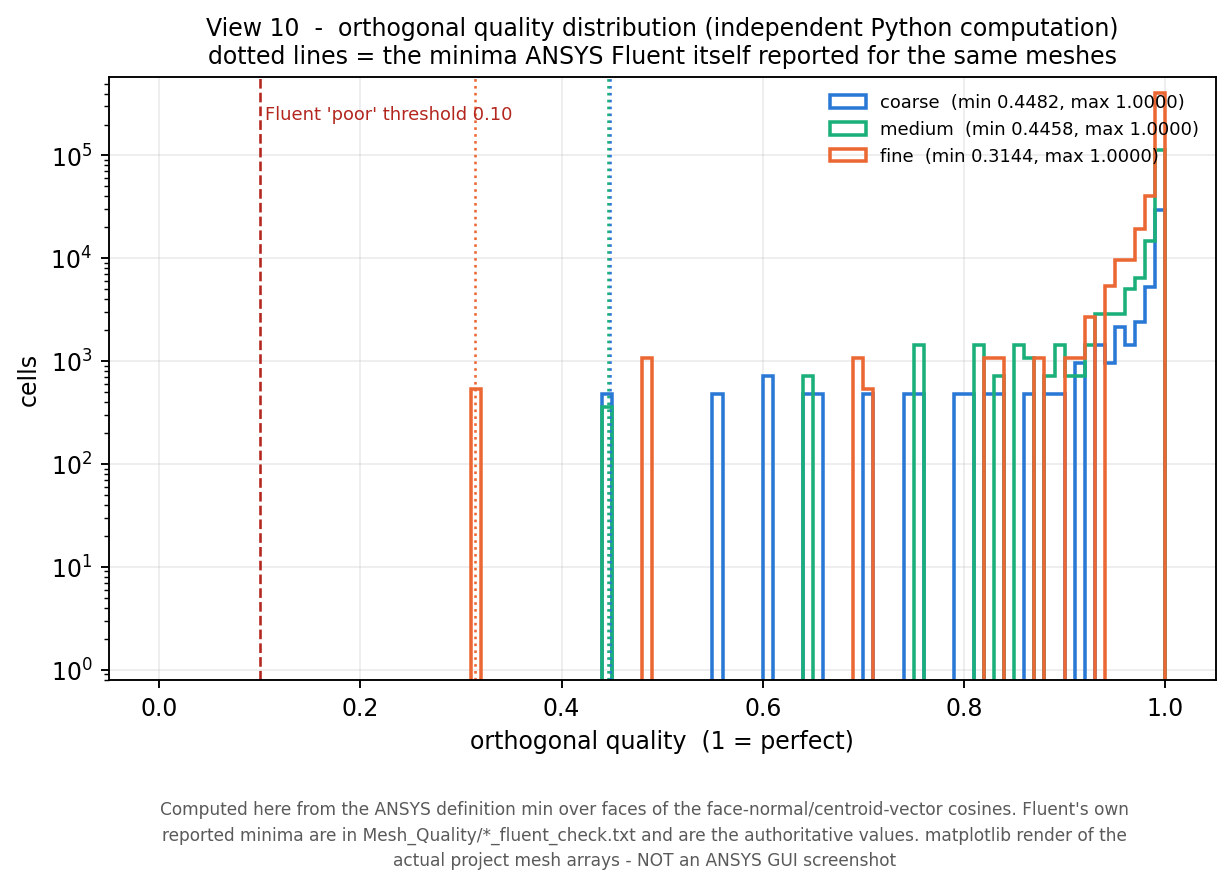
\includegraphics[width=\linewidth]{mesh_10_orthogonal_quality_hist.png}\caption{Orthogonal-quality distribution}\end{subfigure}
\caption[Interface conformity and orthogonal quality of the CFD meshes]{Interface conformity and orthogonal quality of the CFD meshes; dotted lines in (b) mark the minima reported by Fluent.}
\label{fig:meshq}
\src{\provmesh}
\end{figure}

\section{Student-License Constraint}
Fluent Student limited the solver to 4-way parallel execution but stated no cell limit; the 500,580-cell fine mesh was read, checked and
solved. The binding constraint came from the structural side: ANSYS Mechanical Student refuses models above 128,000~nodes (measured:
127,955~nodes solved, 128,045 refused). The fine CFD solid would correspond to about 157\,k structural nodes at 1:1 resolution, beyond that
limit.

\section{Mesh Selection}
The medium mesh (159,840~cells) was selected as the official baseline for all downstream work, and the fine mesh was kept as the
verification reference (decision D-034). The quantitative basis of this choice -- a small and conservative error for the structural phase,
at a third of the cost of the fine mesh -- is given in Chapter~\ref{ch:mi}.

% ===================================================================== Chapter 8
\chapter{Baseline CFD Results}\label{ch:cfdres}
All values in this chapter belong to the official baseline P00 on the medium mesh (159,840~cells) and are summarised in
Table~\ref{tab:cfdres}. They are simulation results of the baseline problem.

%% generated by gen_tables.py - RE-ANALYSIS 2026
\begin{table}[htbp]
\centering
\small
\caption{Baseline CFD results (medium mesh, converged, official baseline P00)}
\label{tab:cfdres}
\begin{tabular}{>{\raggedright\arraybackslash}p{0.50\linewidth}rl}
\toprule
Quantity & Value & Unit \\
\midrule
Cells (fluid + solid) & 159,840 & -- \\
Reynolds number, inlet / outlet & 29,958 / 25,545 & -- \\
Pressure drop (area-weighted static, inlet $-$ outlet) & 438.13 & Pa \\
Outlet bulk temperature (mass-weighted) & 368.93 & K \\
Heat-transfer rate through the heated wall & 602.755 & W \\
Maximum solid temperature (outer-wall facet) & 562.58 & K \\
Maximum solid temperature (hottest cell centre) & 562.13 & K \\
Through-wall $\Delta T$ at mid-span ($z$ = 300 mm) & 7.581 & K \\
Fully developed Nusselt number ($x/D$ 18--29) & 54.17 & -- \\
Fully developed Darcy friction factor ($x/D$ 18--29) & 0.02163 & -- \\
$y^+$ minimum / area mean / maximum & 0.208 / 0.241 / 0.585 & -- \\
Mass imbalance / energy imbalance & $7.0\times10^{-13}$ / $3.1\times10^{-11}$ & \% \\
\bottomrule
\end{tabular}
\par\smallskip\parbox{\linewidth}{\footnotesize\raggedright Source: \texttt{MASTER\_PROJECT\_DATA.csv} rows M033--M048 (VERIFIED from the Fluent flux and surface-integral reports, except M035 REPORTED and M041--M043 CROSS-CHECKED). $Q$ = 602.755~W is 8000~W/m$^2$ times the inscribed 48-gon area; the same flux on the true cylinder is 603.186~W.}
\end{table}


\section{Convergence}
The solution converged at iteration 600 and was confirmed at iteration 700 (Figure~\ref{fig:conv}). The evaluation at iteration 500 was
refused because the 200-iteration window still contained the transient caused by the switch to second-order schemes (outlet temperature
drift 0.42~K). The residuals fell to round-off level (continuity $9.0\times10^{-11}$, energy $1.6\times10^{-14}$); the evidence of convergence,
however, is the physical monitors, which are flat to within $10^{-5}$ K. The solid temperature rose monotonically during the energy stage,
without overshoot.

\begin{figure}[htbp]
\centering
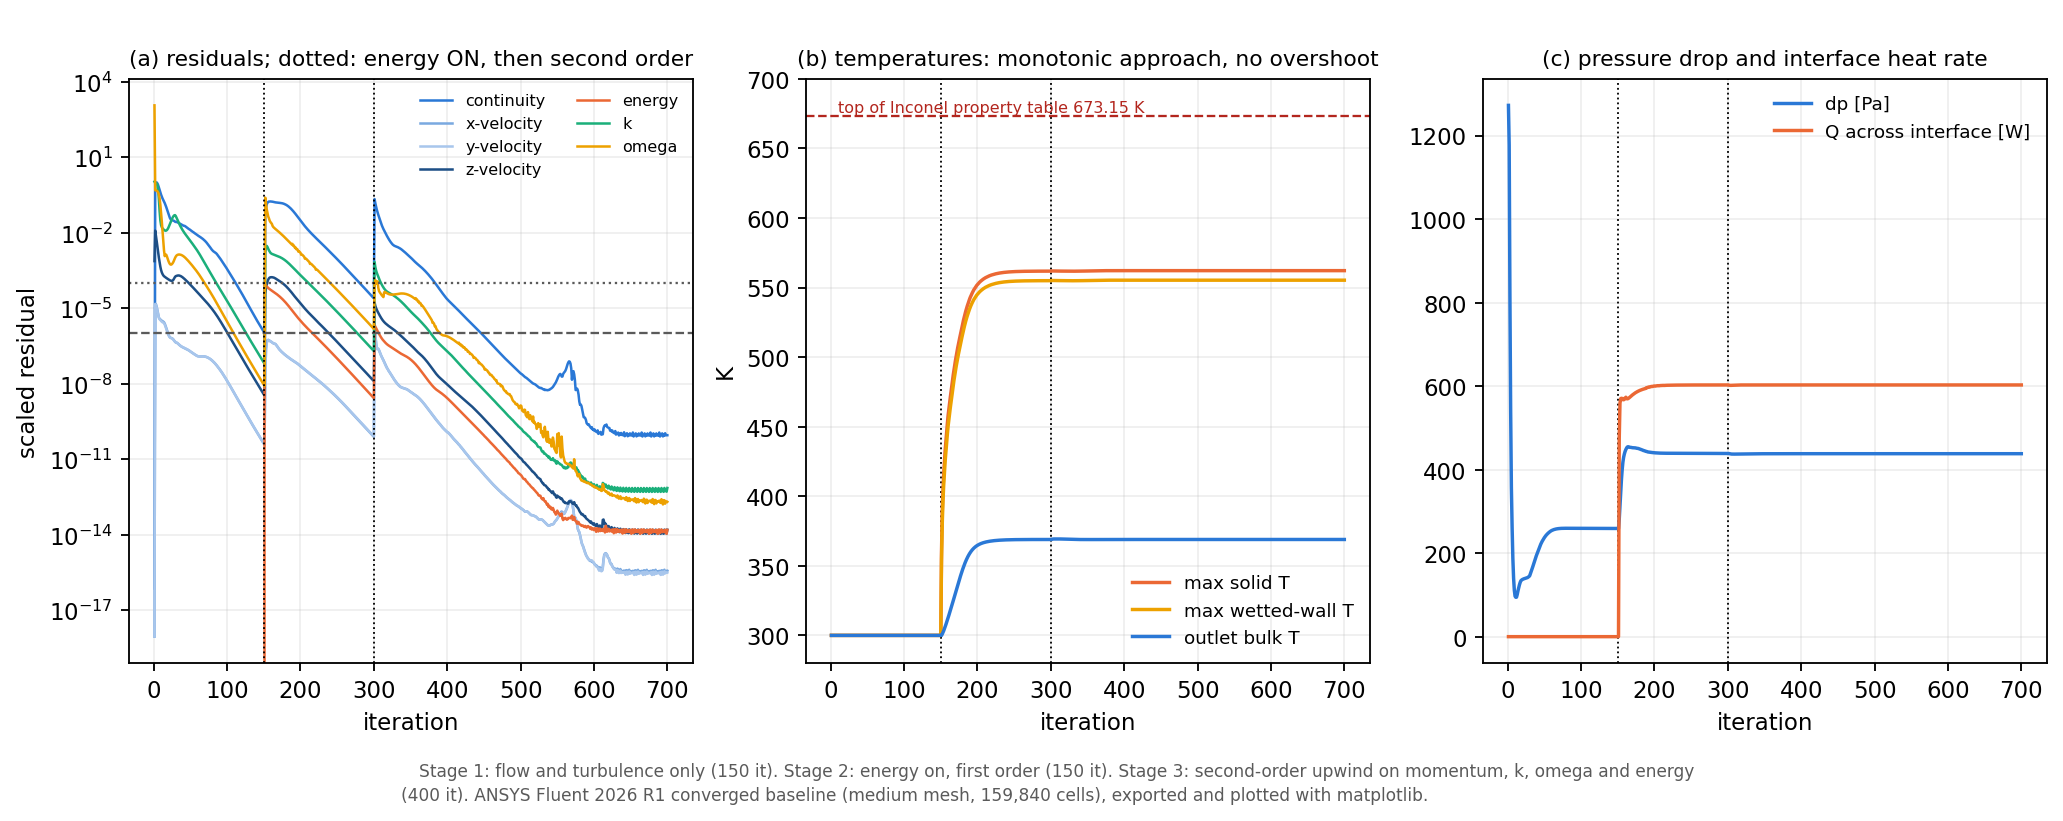
\includegraphics[width=0.90\linewidth]{fig16_convergence_nt.png}
\caption[Convergence history of the baseline run]{Convergence history of the baseline run: (a) scaled residuals, (b) monitored temperatures, (c) pressure drop and interface heat rate.
Stage boundaries at iterations 150 (energy on) and 300 (second-order schemes).}
\label{fig:conv}
\src{\provcfd}
\end{figure}

\section{Mass Conservation}
Inlet and outlet mass flow are both 8.662155~g/s; the Fluent flux report gives a mass imbalance of $7.0\times10^{-13}$\,\% of the flow. The mass
flow is 0.28\,\% below the analytical 8.686~g/s, which is entirely explained by the inscribed-polygon inlet area (area ratio 0.997147) and the
gas constant used by Fluent. No reverse-flow cell or outlet face occurred.

\section{Energy Conservation}
The heat entering the outer wall (602.755~W) crosses the interface to within $9\times10^{-10}$ W and leaves with the air: the enthalpy flux rises
from 16.107 to 618.862~W. The net energy imbalance over all boundaries is $3.1\times10^{-11}$\,\% of $Q$. The 0.071\,\% difference from the
analytical 603.186~W is exactly the ratio of the 48-gon lateral area to the cylinder area.

\section{Velocity Field}
The uniform inlet profile develops into a turbulent profile (Figure~\ref{fig:vel}). The ratio of maximum to bulk velocity reaches 98\,\% of its
exit value at $x/D \approx 17.8$. Because heating lowers the density by about 19\,\% along the duct, the flow accelerates: the area-mean
velocity rises from 23.500~m/s to 28.894~m/s and the maximum velocity, 34.99~m/s, occurs on the outlet centreline. Radial and swirl
velocities stay below 0.54~m/s and 0.013~m/s; secondary flow is negligible.

\begin{figure}[htbp]
\centering
\begin{subfigure}[t]{0.49\linewidth}\centering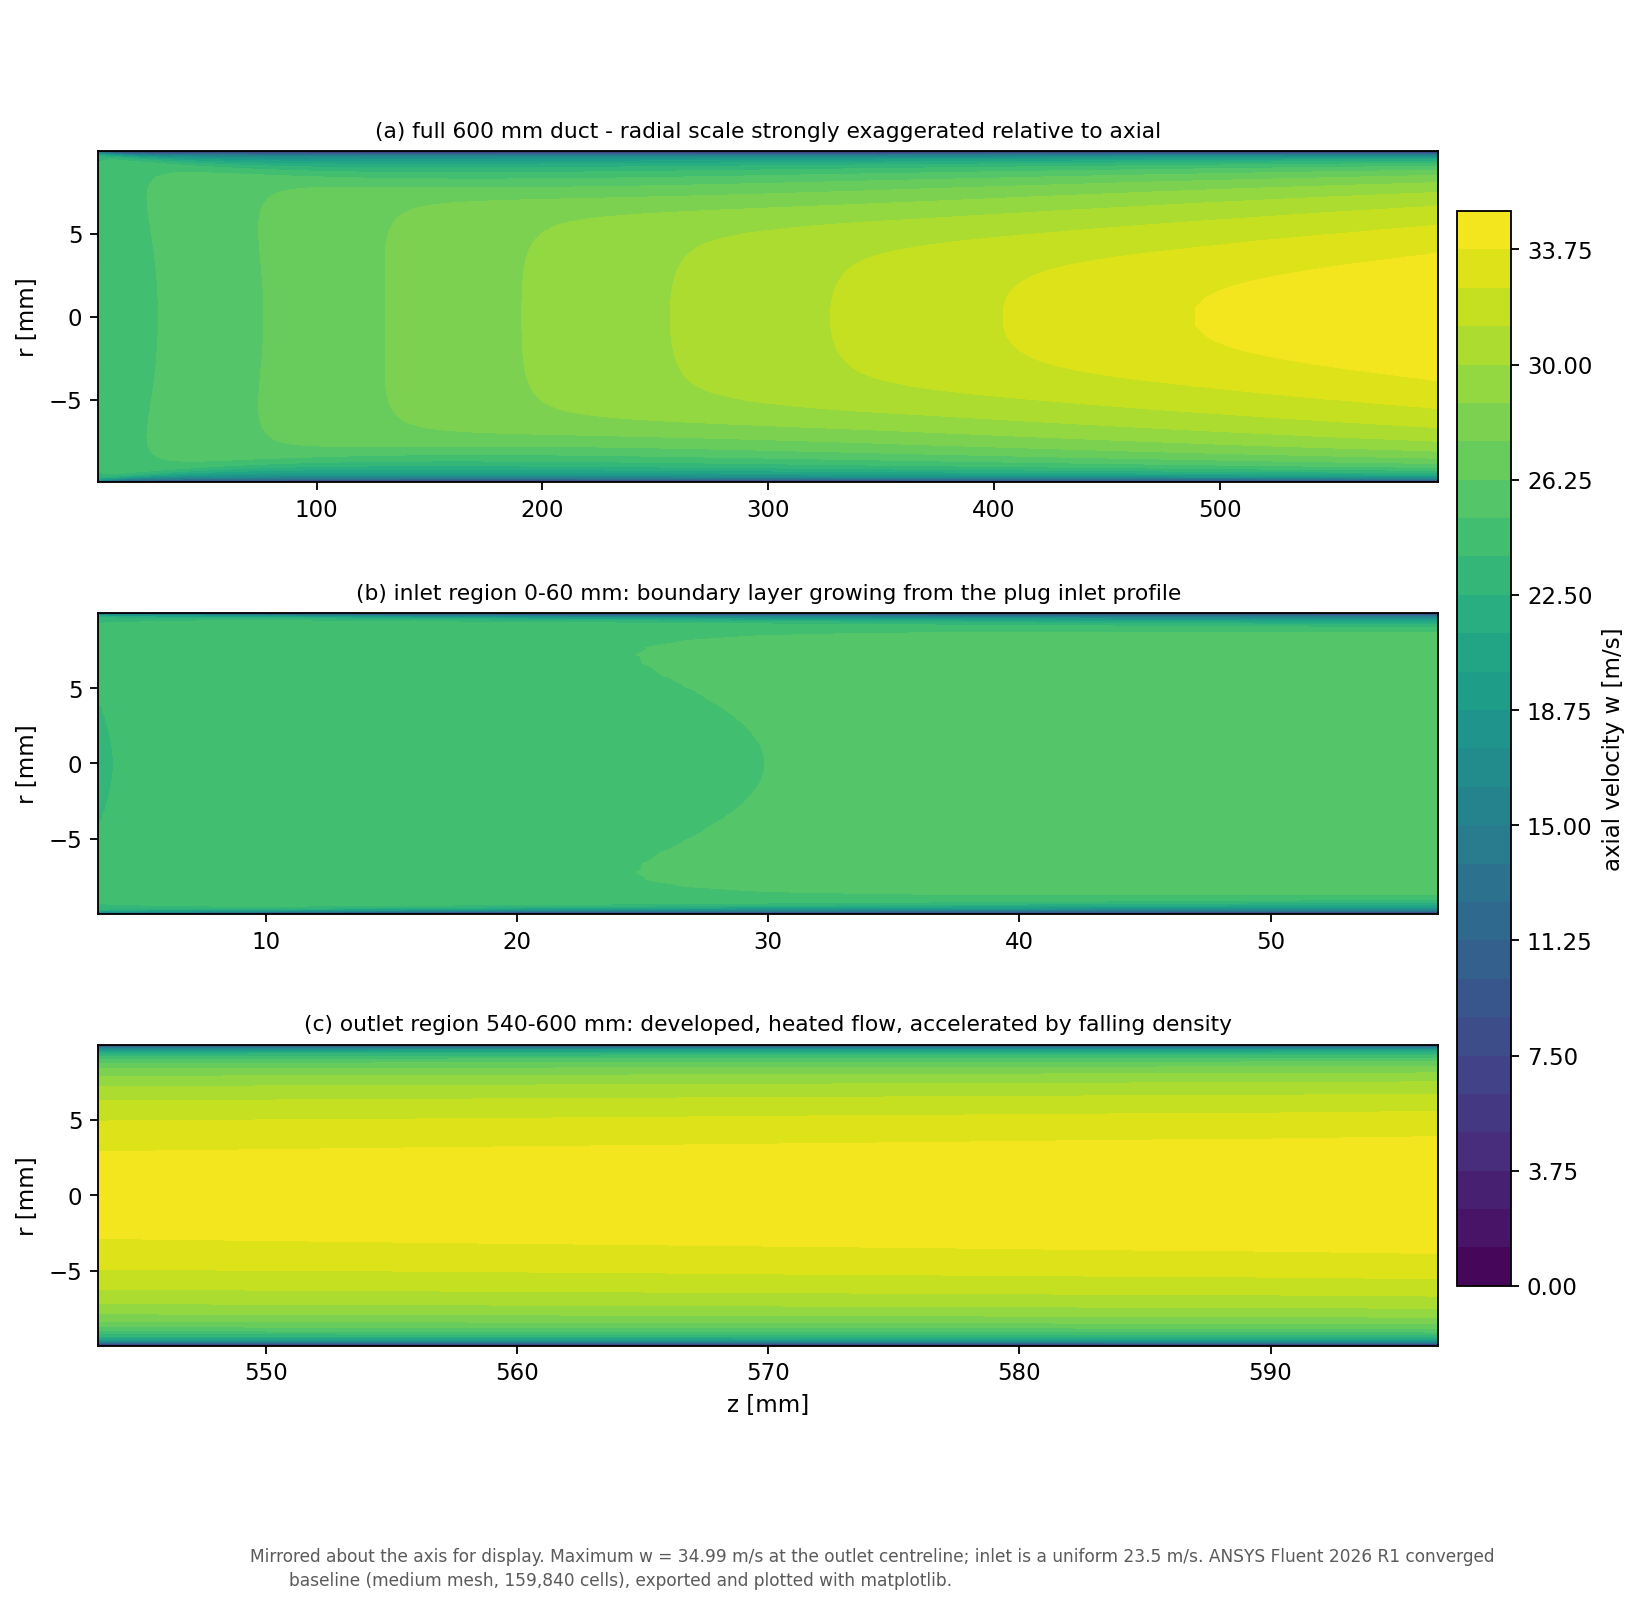
\includegraphics[width=\linewidth,height=52mm,keepaspectratio]{fig01_velocity_contour_nt.png}\caption{Axial velocity (radial scale exaggerated) [m/s]}\end{subfigure}\hfill
\begin{subfigure}[t]{0.49\linewidth}\centering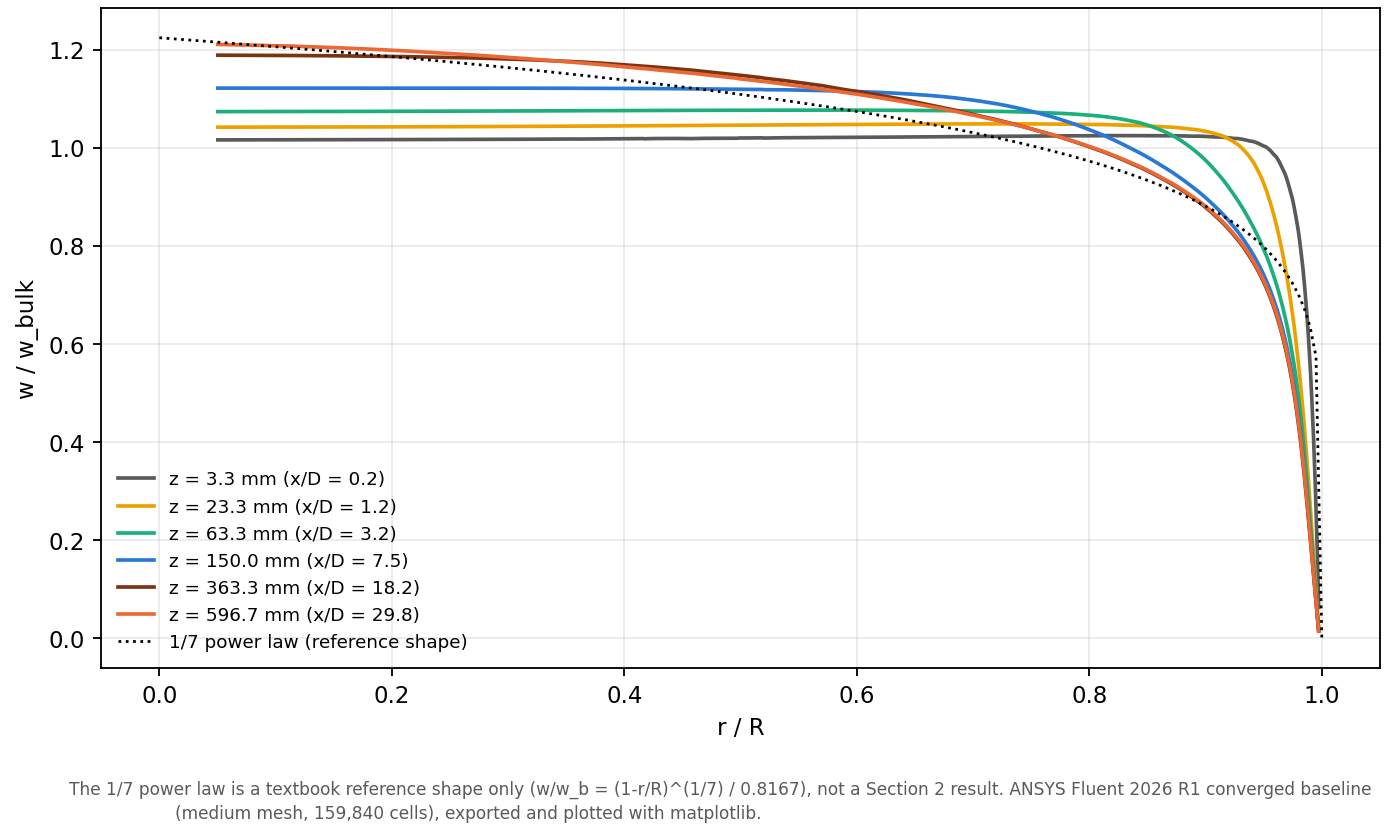
\includegraphics[width=\linewidth,height=52mm,keepaspectratio]{fig13_velocity_profiles_nt.png}\caption{Normalised axial-velocity profiles $w/w_b$}\end{subfigure}
\caption[Velocity field of the baseline]{Velocity field of the baseline: development from the uniform inlet profile to a turbulent profile, and acceleration of the heated air.}
\label{fig:vel}
\src{\provcfd{} The 1/7 power law in (b) is a textbook reference shape only.}
\end{figure}

\section{Pressure Field}
The static pressure is almost uniform over each cross-section and falls monotonically from 438.13~Pa (area average at the inlet) to 0~Pa
gauge at the outlet (Figure~\ref{fig:press}). The gradient is steepest in the entry region, where the boundary layer is thin, and steepens
again downstream as heating accelerates the air. An axial momentum balance on the exported field decomposes the drop into wall shear
(242.87~Pa), one-dimensional acceleration (149.31~Pa) and momentum-flux profile development (46.15~Pa), closing to $-$0.045\,\%.

\begin{figure}[htbp]
\centering
\begin{subfigure}[t]{0.52\linewidth}\centering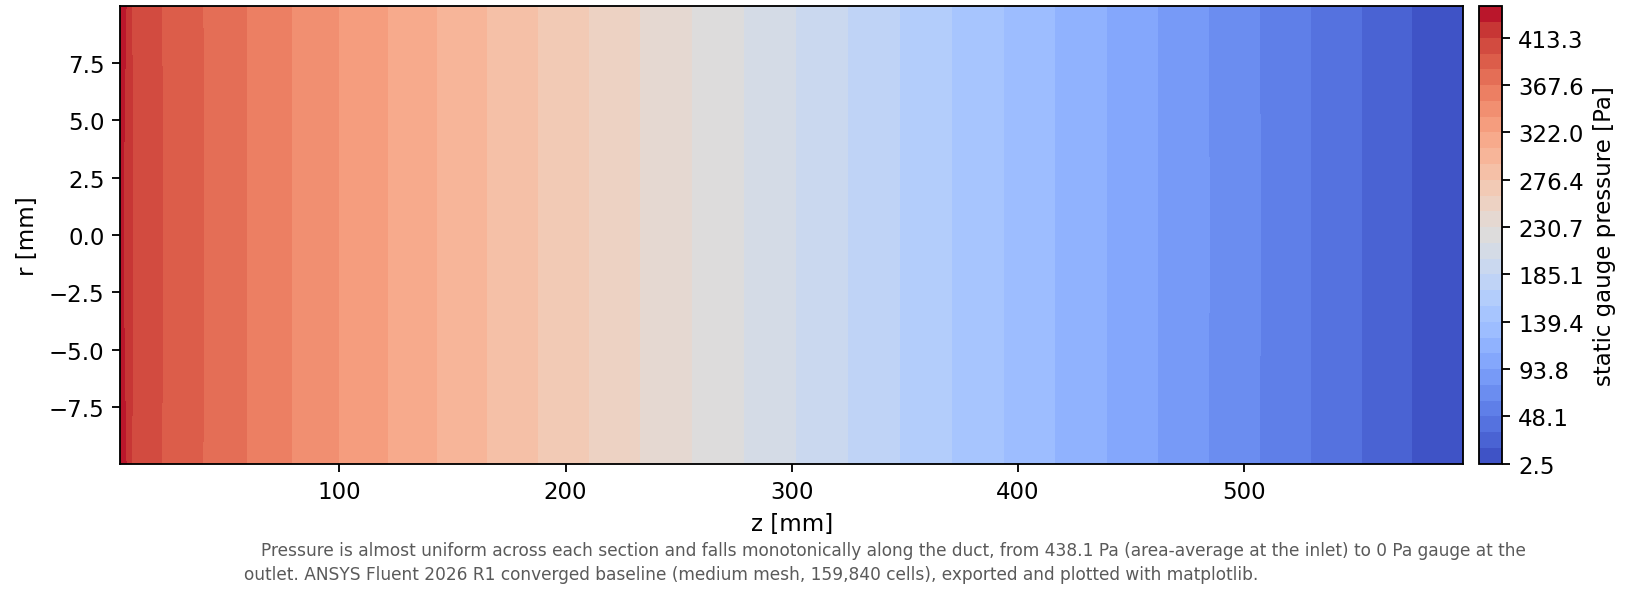
\includegraphics[width=\linewidth,height=52mm,keepaspectratio]{fig04_pressure_contour_nt.png}\caption{Static gauge pressure [Pa]}\end{subfigure}\hfill
\begin{subfigure}[t]{0.46\linewidth}\centering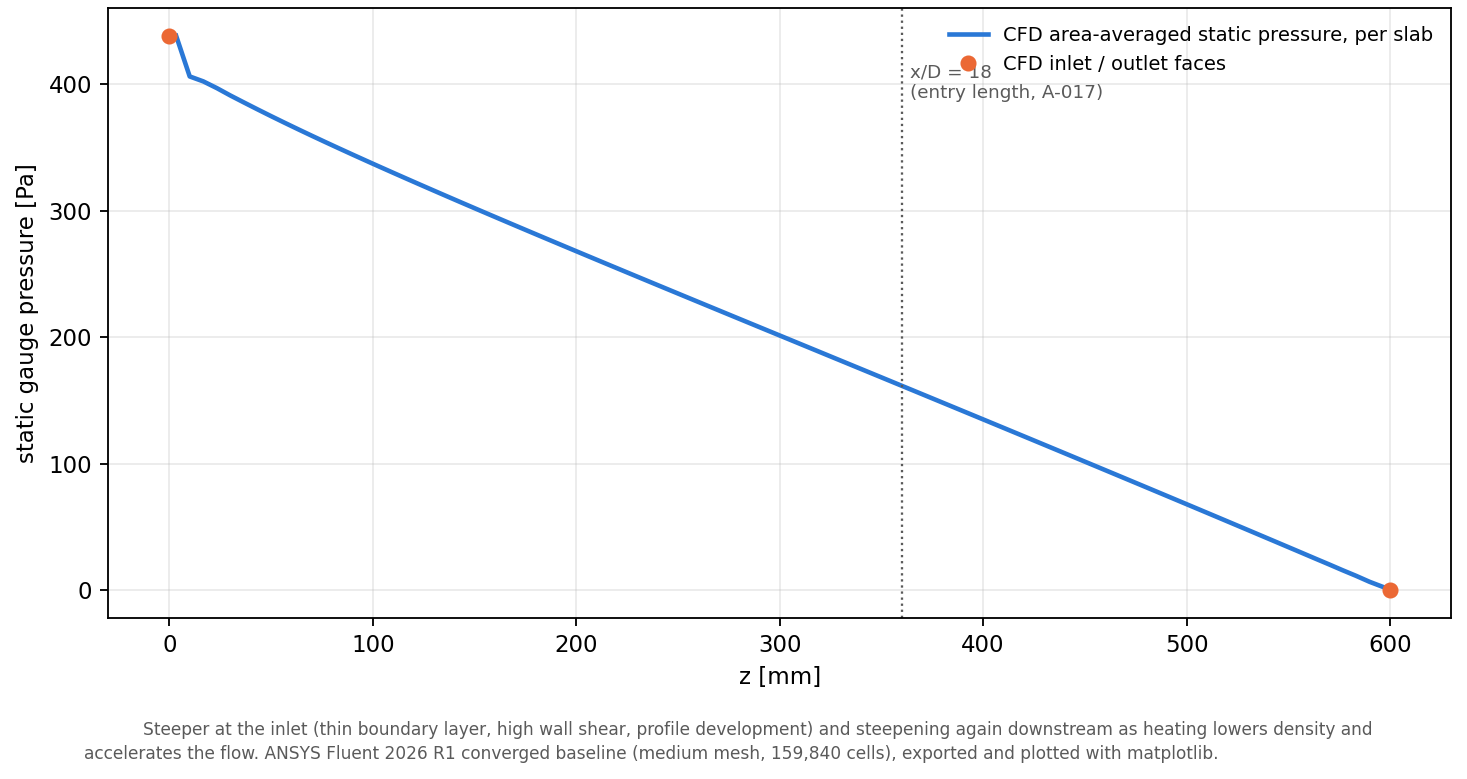
\includegraphics[width=\linewidth,height=52mm,keepaspectratio]{fig10_pressure_axial_nt.png}\caption{Area-averaged static pressure along the duct}\end{subfigure}
\caption[Pressure field of the baseline]{Pressure field of the baseline: inlet-to-outlet static pressure drop of 438.13~Pa.}
\label{fig:press}
\src{\provcfd}
\end{figure}

\section{Temperature Field}
The air heats almost linearly along the duct, from 300~K to a mass-weighted outlet temperature of 368.93~K (Figures~\ref{fig:temp}
and~\ref{fig:taxial}a). The heated layer is thin: at the outlet a hot wall layer surrounds a core that is still close to the bulk temperature.
The solid ranges from 423.97~K (inlet end) to 562.58~K (medium mesh) at the outer-wall facet near the adiabatic outlet end; the hottest cell centre is at
562.13~K and the volume-mean solid temperature is 525.48~K. The through-wall temperature difference is 7.581~K at mid-span and 7.361~K at
$z$ = 570~mm, but rises to 15.1~K in the first axial slab, where the cold air and thin thermal boundary layer draw heat axially through the
wall towards the inlet (Figure~\ref{fig:taxial}b).

\begin{figure}[htbp]
\centering
\begin{subfigure}[t]{0.40\linewidth}\centering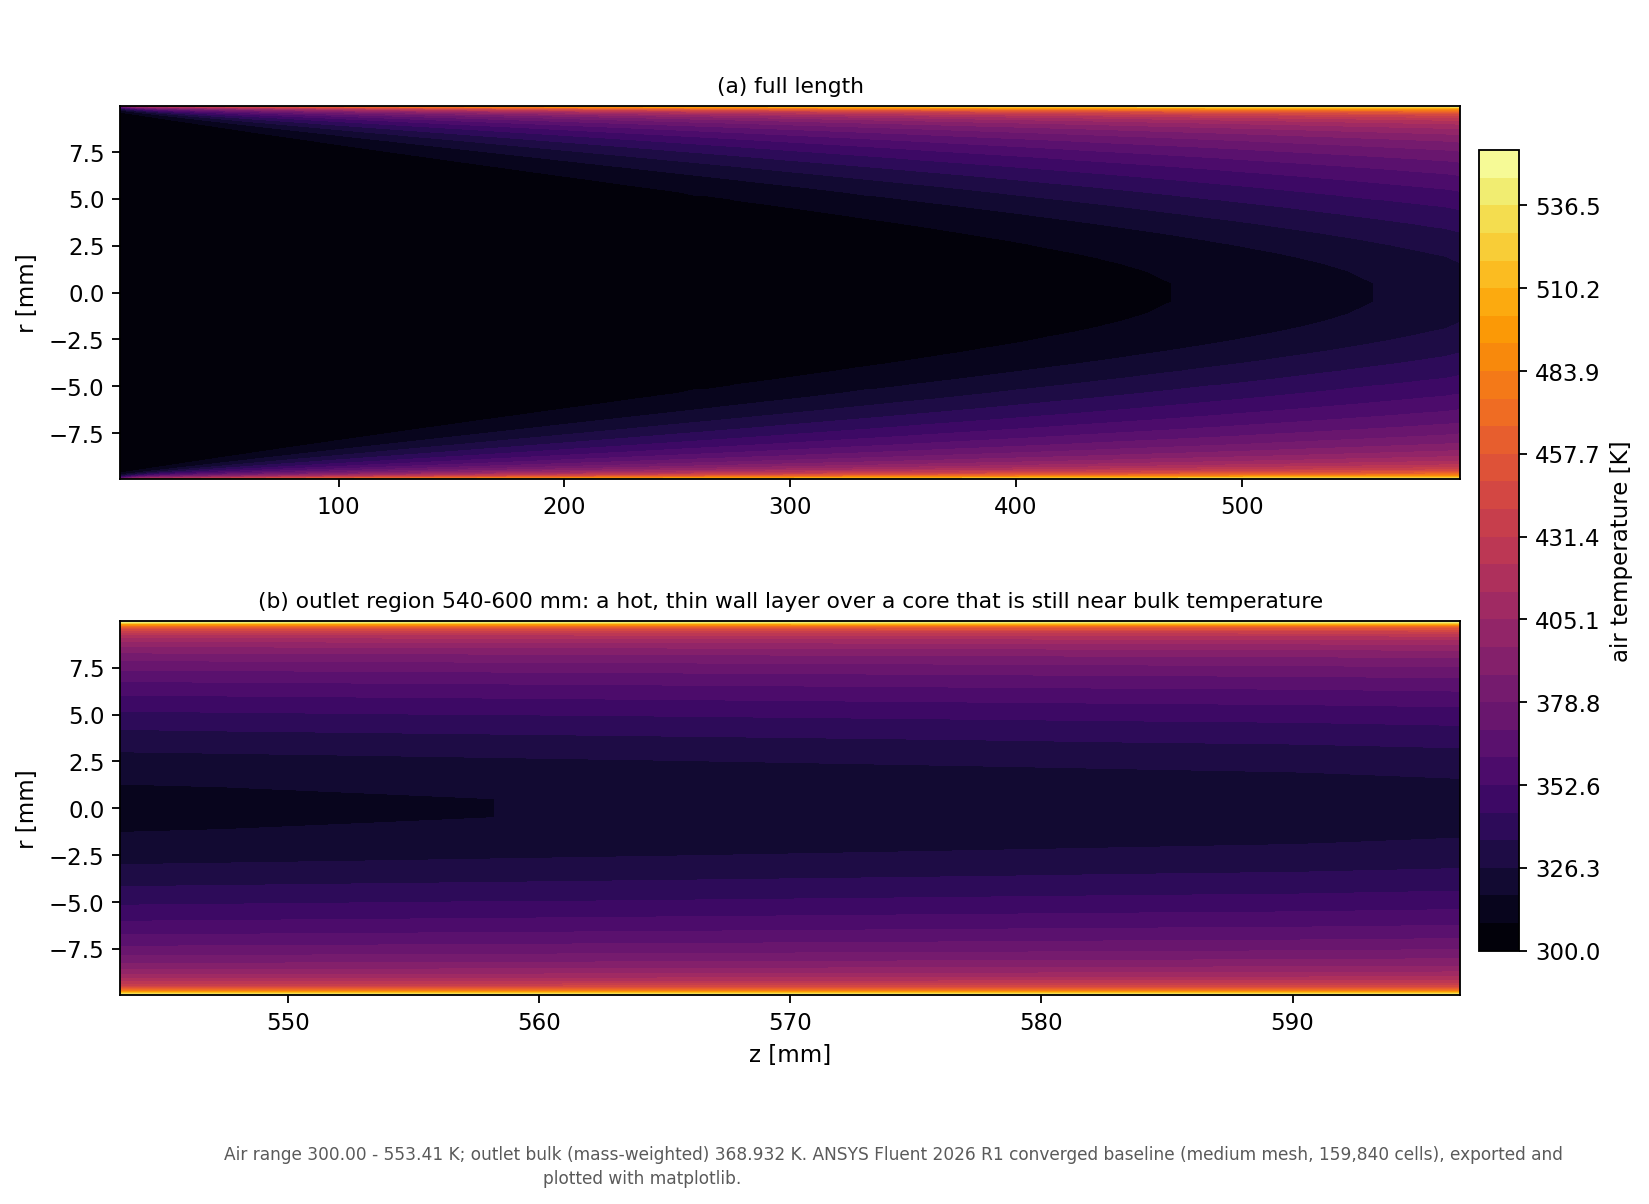
\includegraphics[width=\linewidth,height=52mm,keepaspectratio]{fig05_fluid_temperature_contour_nt.png}\caption{Air temperature [K]}\end{subfigure}\hfill
\begin{subfigure}[t]{0.58\linewidth}\centering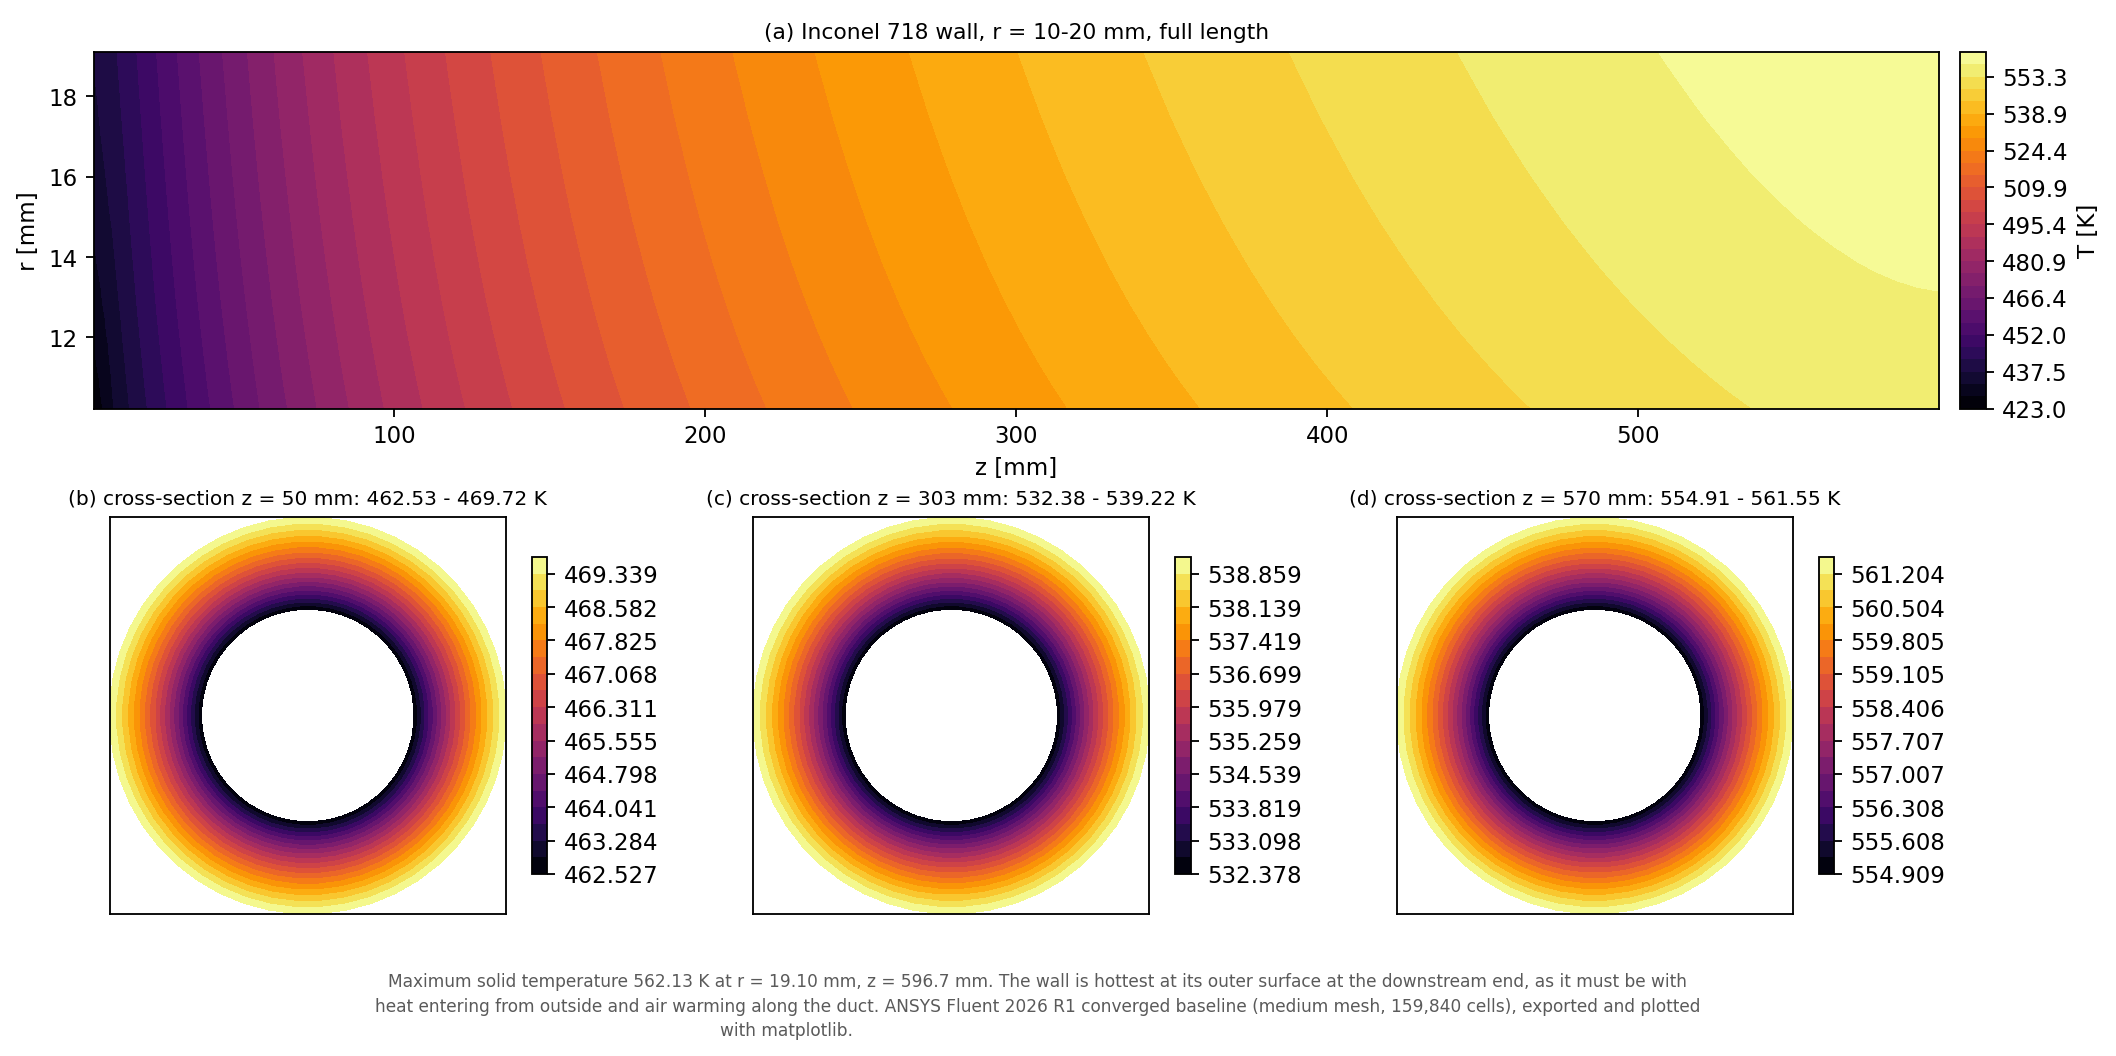
\includegraphics[width=\linewidth,height=52mm,keepaspectratio]{fig06_solid_temperature_contour_nt.png}\caption{Inconel 718 wall temperature [K]}\end{subfigure}
\caption{Temperature field of the baseline in the meridional plane (radial scale exaggerated) and in three wall cross-sections.}
\label{fig:temp}
\src{\provcfd}
\end{figure}

\begin{figure}[htbp]
\centering
\begin{subfigure}[t]{0.48\linewidth}\centering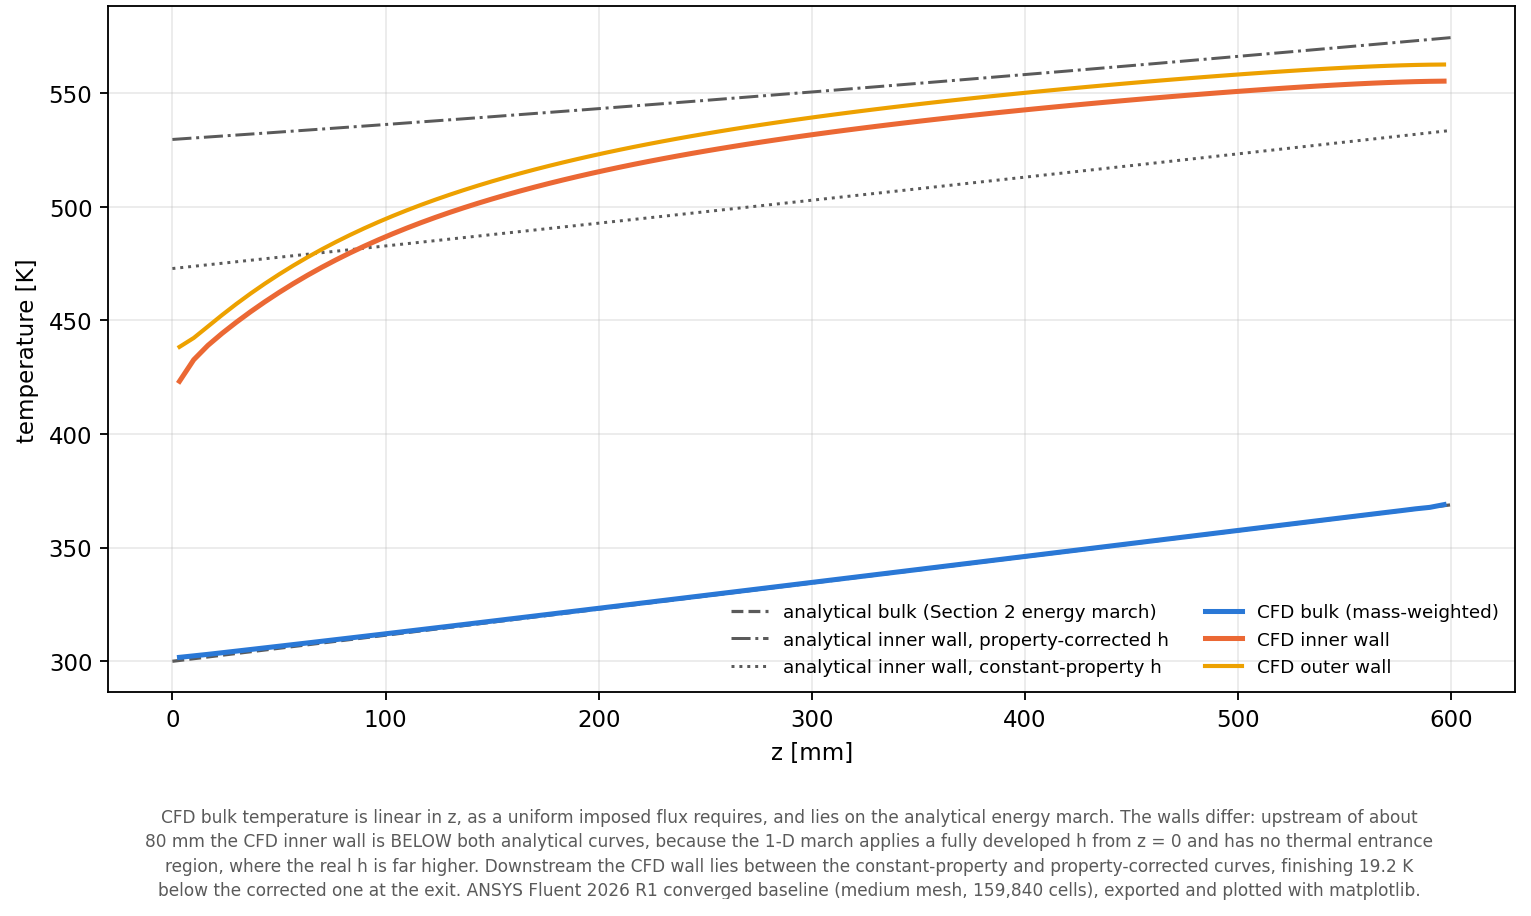
\includegraphics[width=\linewidth,height=52mm,keepaspectratio]{fig11_bulk_temperature_axial_nt.png}\caption{Bulk and wall temperatures, CFD and analytical}\end{subfigure}\hfill
\begin{subfigure}[t]{0.50\linewidth}\centering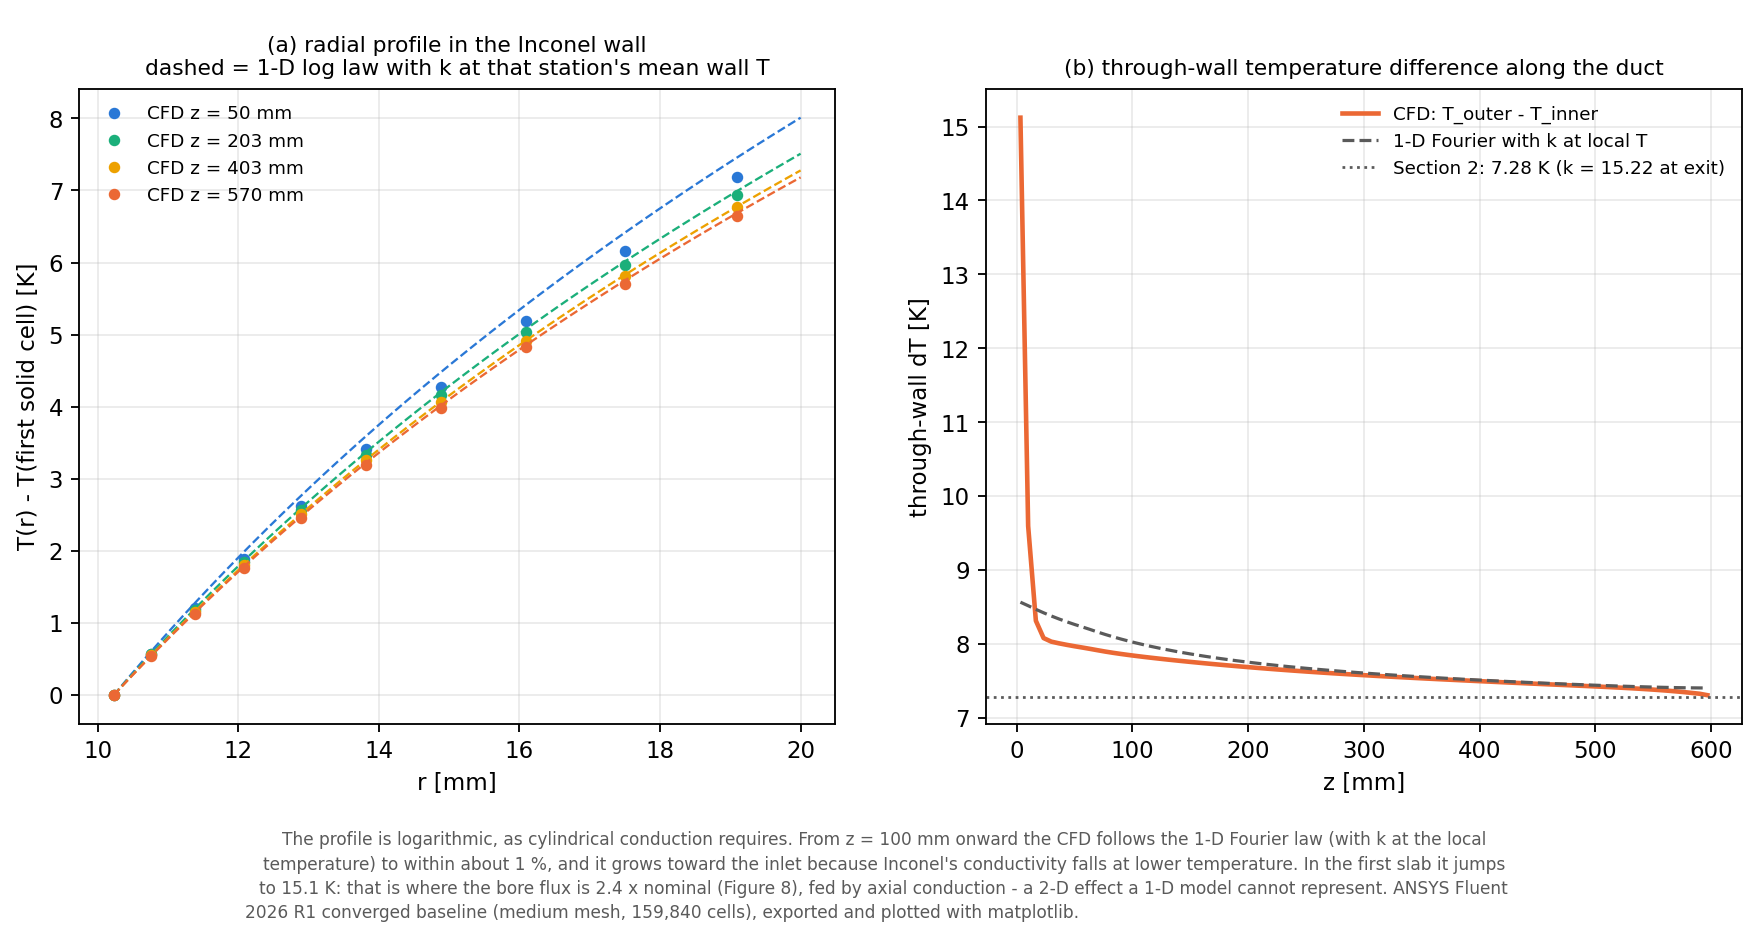
\includegraphics[width=\linewidth,height=52mm,keepaspectratio]{fig12_through_wall_temperature_nt.png}\caption{Radial profile and through-wall $\Delta T$ along the duct}\end{subfigure}
\caption[Axial temperature development and through-wall temperature difference]{Axial temperature development and through-wall temperature difference. Dashed and dotted lines are the Section 2 analytical estimates.}
\label{fig:taxial}
\src{\provcfd}
\end{figure}

\section{Heat Transfer}
Heat enters uniformly at 8000~W/m$^2$ on the outside but does not leave uniformly at the bore (Figure~\ref{fig:flux}a). In the first slab
the bore flux reaches 38,471~W/m$^2$, 2.4 times the one-dimensional 16,000~W/m$^2$, because the heat-transfer coefficient is very high in the
thermal entrance region; it recovers to within 1\,\% of 16,000~W/m$^2$ by $z \approx$ 250~mm. Figure~\ref{fig:flux}b shows that almost the
whole wall-to-bulk temperature difference lies in the thin air layer next to the wall: the 10~mm of Inconel carries only a few kelvin.
This is the Section 2 finding that the film carries about 97\,\% of the thermal resistance, seen directly in the solution.

\begin{figure}[htbp]
\centering
\begin{subfigure}[t]{0.54\linewidth}\centering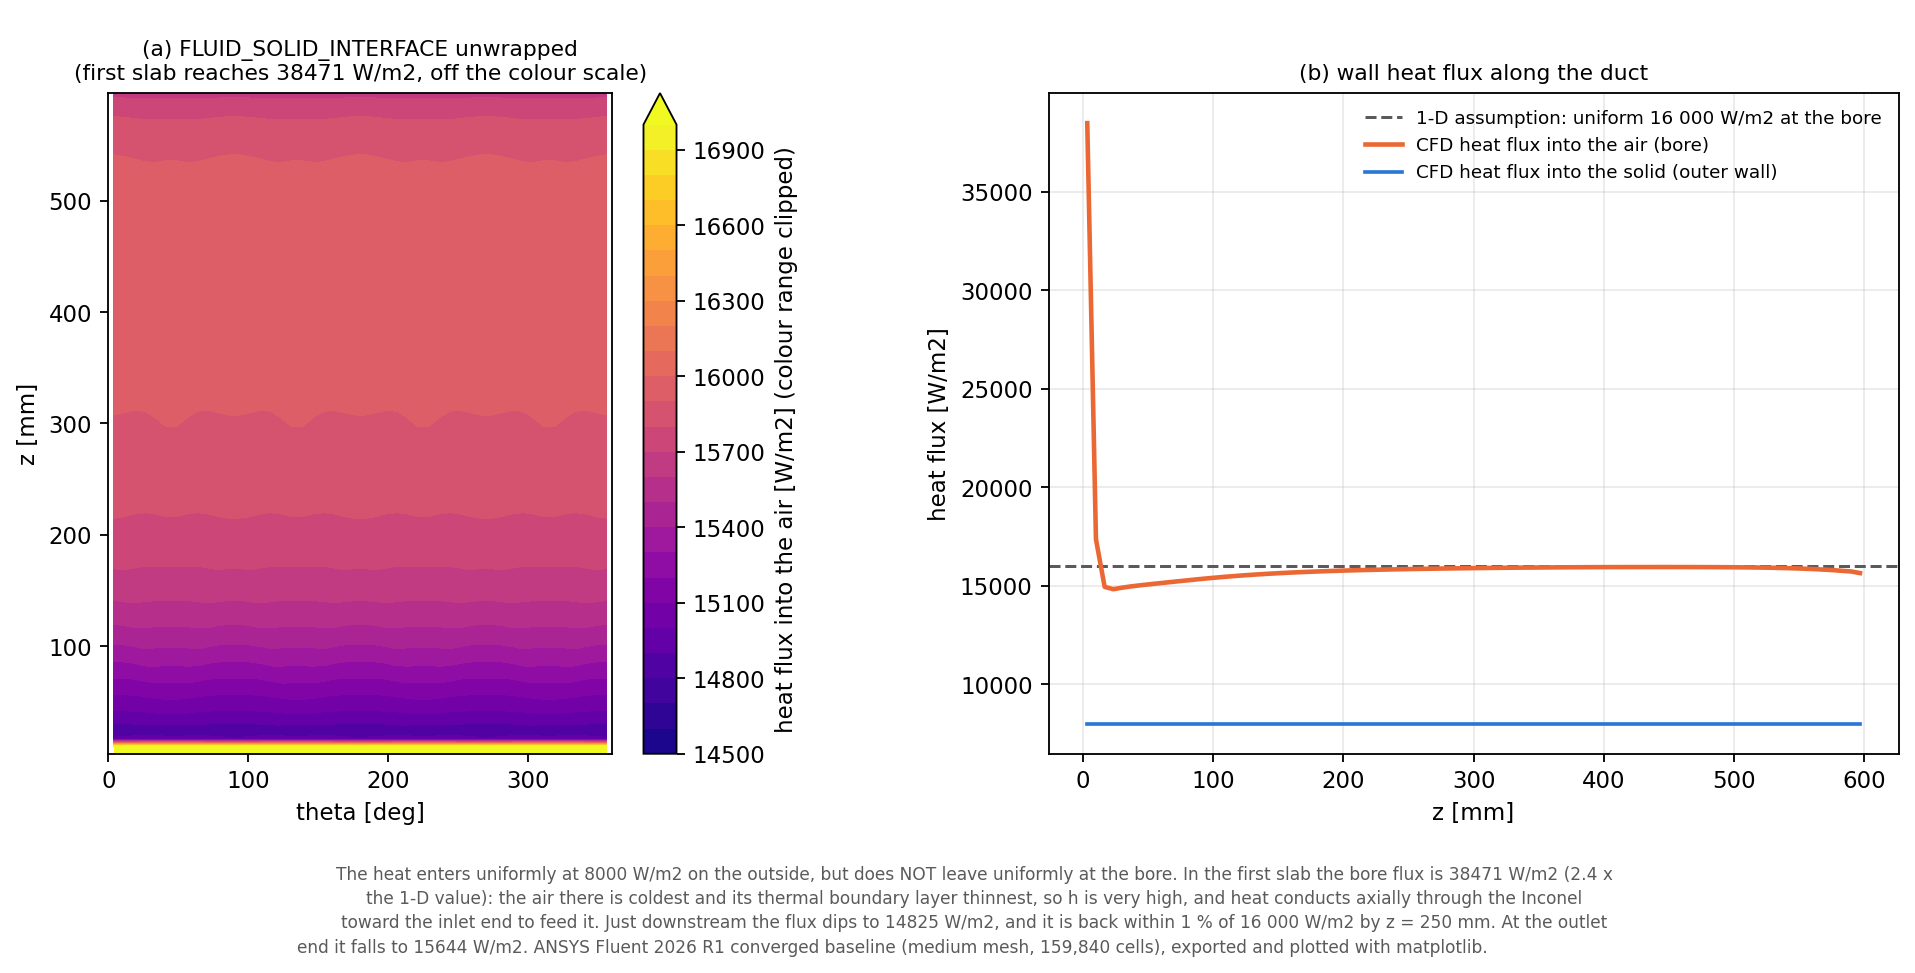
\includegraphics[width=\linewidth,height=52mm,keepaspectratio]{fig08_wall_heat_flux_nt.png}\caption{Wall heat flux [W/m$^2$]}\end{subfigure}\hfill
\begin{subfigure}[t]{0.44\linewidth}\centering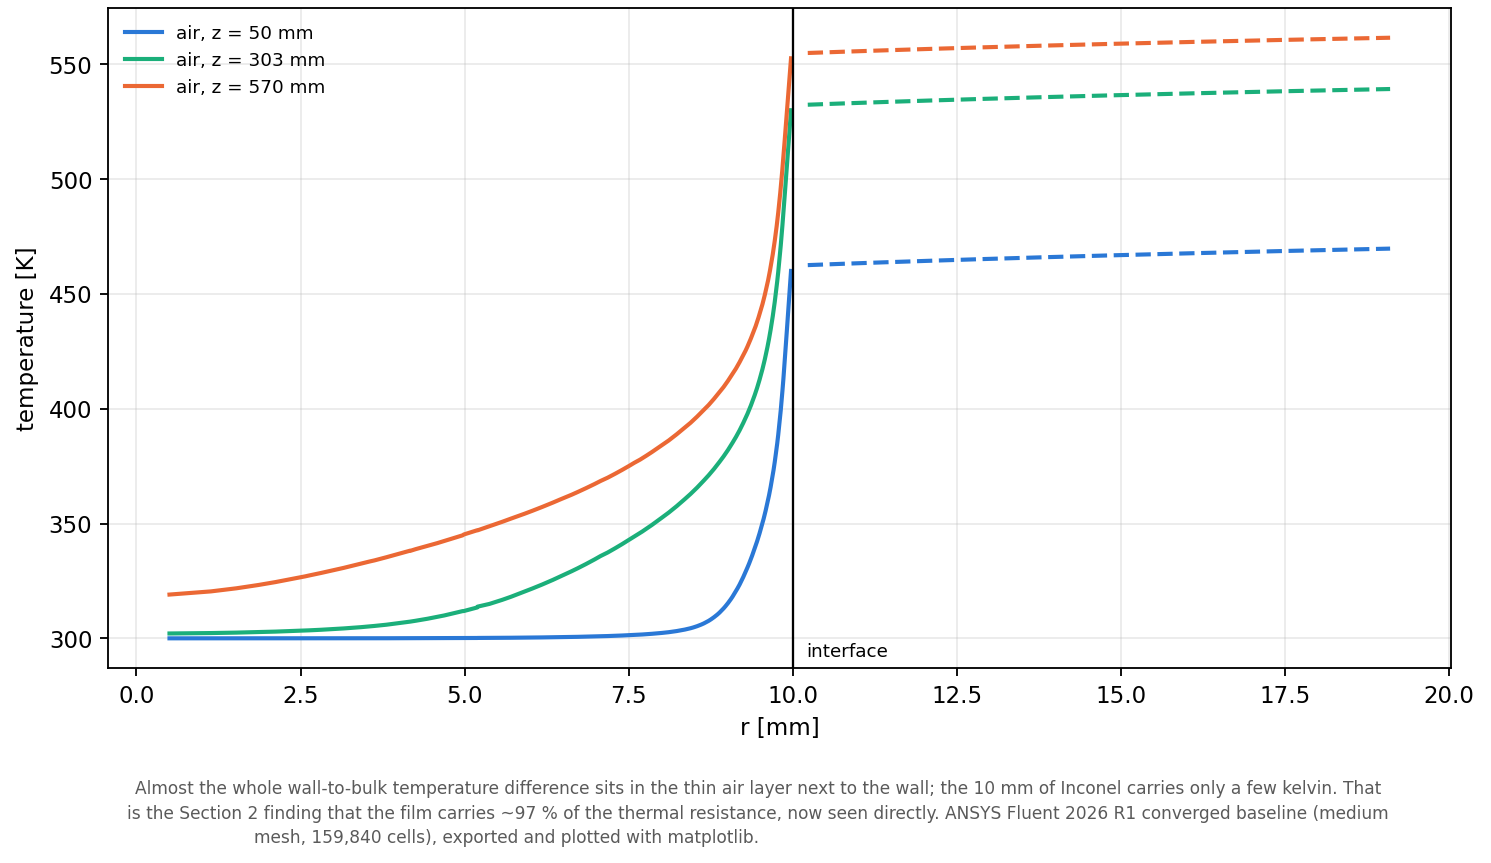
\includegraphics[width=\linewidth,height=52mm,keepaspectratio]{fig14_radial_temperature_nt.png}\caption{Radial temperature in air and wall}\end{subfigure}
\caption{Heat-flux distribution at the interface and radial temperature distribution at three stations.}
\label{fig:flux}
\src{\provcfd}
\end{figure}

\section{Nusselt Number}
Over the fully developed window $x/D$ = 18--29 the mean Nusselt number is 54.17 (Figure~\ref{fig:nuf}a); the corresponding film coefficient
near the outlet is 83.6~W/(m$^2$\,K). The value lies between the property-corrected correlation (51.0 at the CFD conditions) and the
constant-property correlations (Gnielinski 63.5, Dittus--Boelter 68.6), and inside the expected band of 44--67. The CFD implies a
property-ratio exponent of about 0.36 instead of the 0.5 assumed in the analytical model.

\begin{figure}[htbp]
\centering
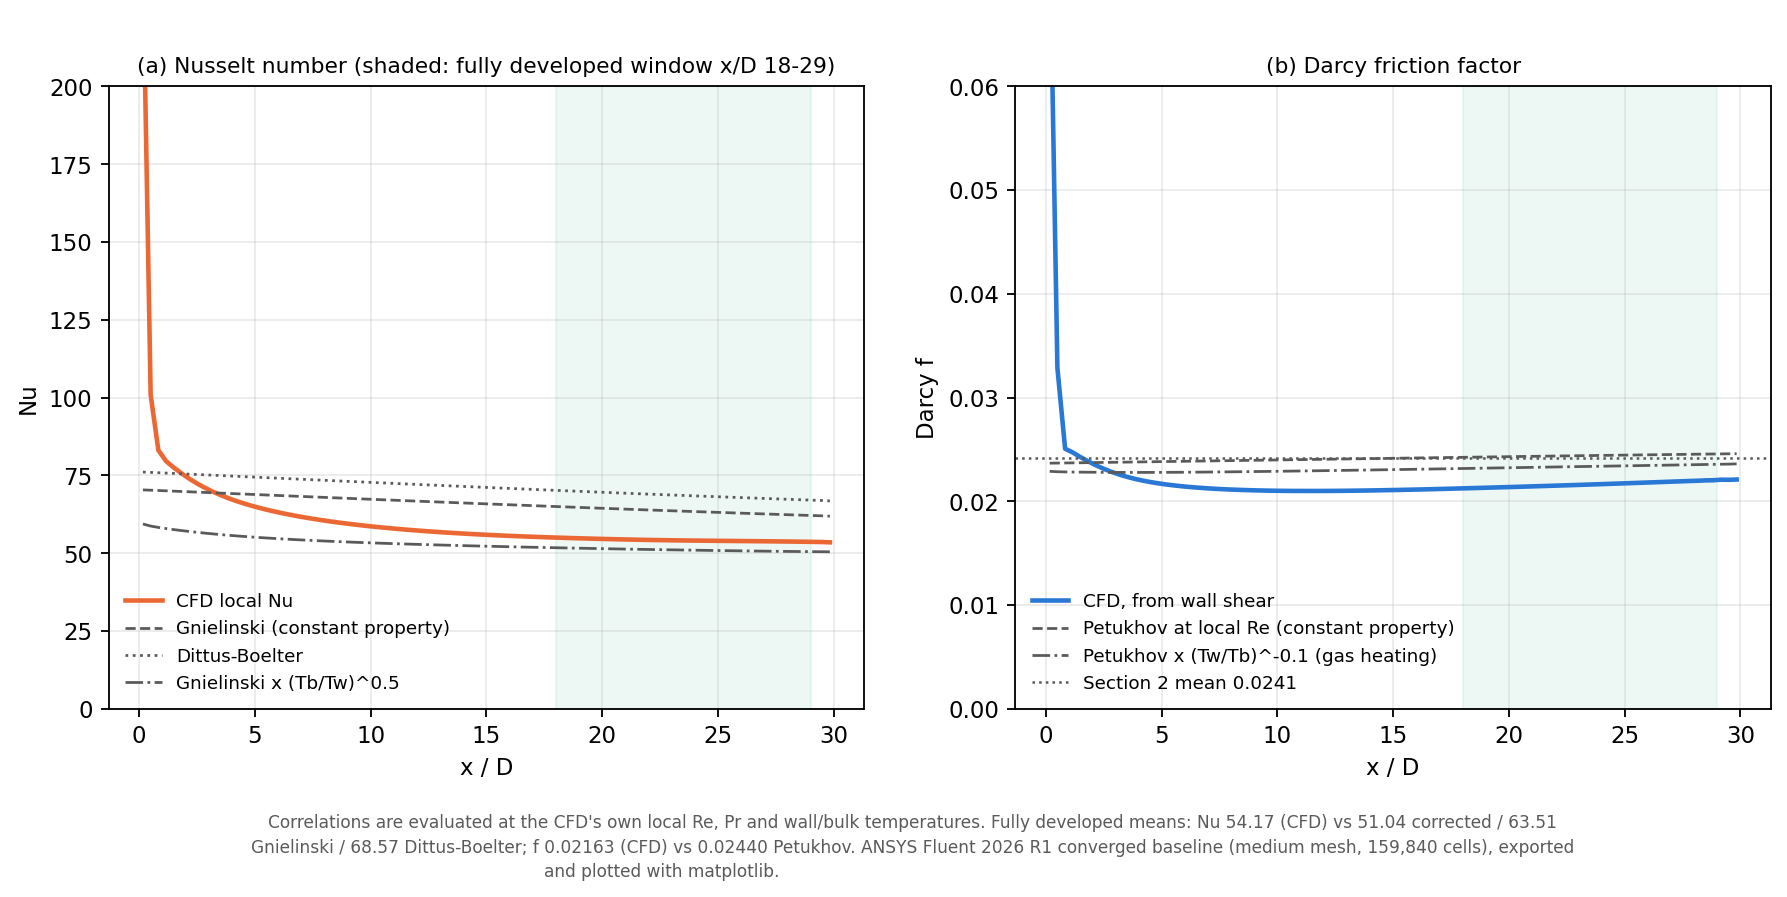
\includegraphics[width=0.78\linewidth]{fig15_nusselt_friction_nt.png}
\caption[Local Nusselt number (a) and Darcy friction factor (b) along the duct compared with correlations]{Local Nusselt number (a) and Darcy friction factor (b) along the duct compared with correlations; the shaded band is the fully developed window $x/D$ = 18--29.}
\label{fig:nuf}
\src{\provcfd}
\end{figure}

\section{Friction Factor}
The fully developed Darcy friction factor, $f = 8\tau_w\rho_b/G^2$ over the same window, is 0.02163, 10.4\,\% below the Petukhov value of
0.0241 (Figure~\ref{fig:nuf}b). This marginally misses the $\pm$10\,\% requirement set in Section 1 (PR-04), which is recorded rather than
re-interpreted. The mesh study (Chapter~\ref{ch:mi}) traces the difference mainly to gas heating: the variable-property effect reduces the
friction factor by a factor of 0.910 beyond the constant-property Reynolds-number change, which the constant-property correlation omits.

\section{y+}\label{sec:yplus}
On the conjugate wall $y^+$ ranges from 0.208 to 0.585 with an area mean of 0.241 (Figure~\ref{fig:yplus}); 100\,\% of the area has
$y^+ \le 1$ and 99.07\,\% has $y^+ \le 0.5$. The maximum occurs in the first slab, where the wall shear is highest. Wall shear and wall heat
flux are therefore resolved, not modelled by a wall function.

\begin{figure}[htbp]
\centering
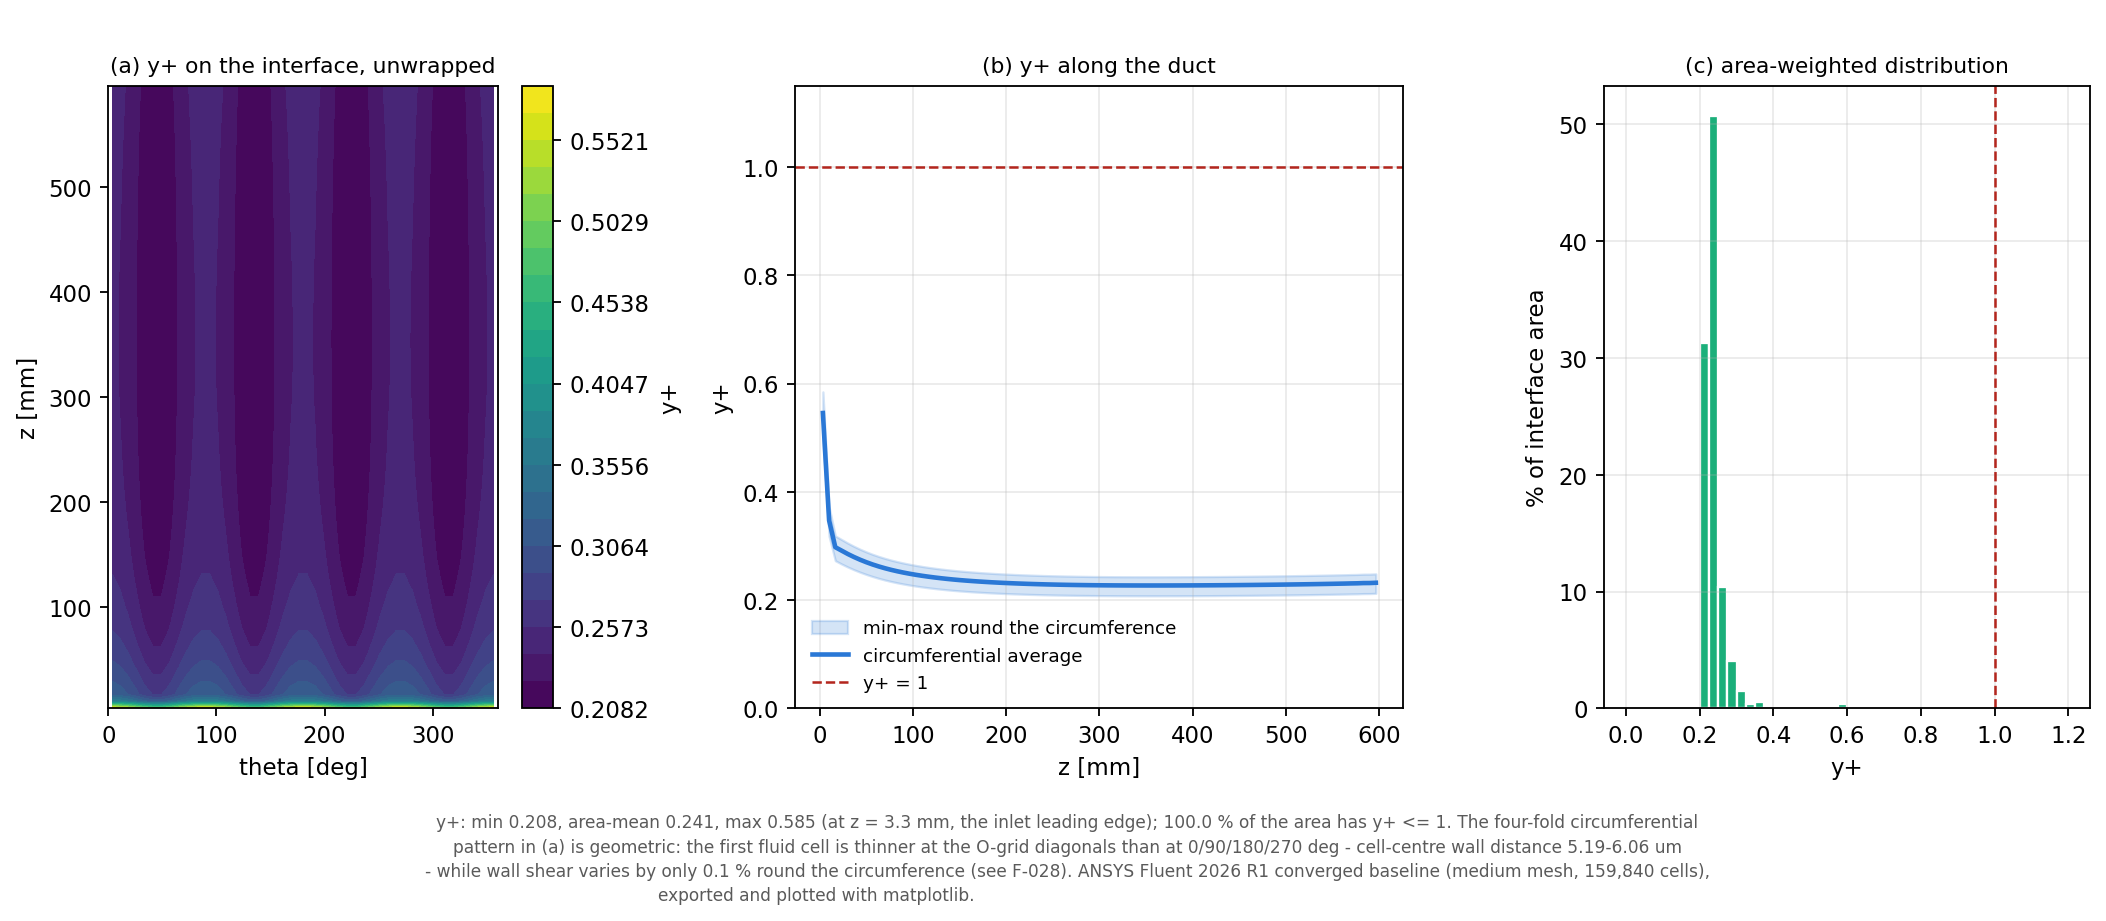
\includegraphics[width=0.85\linewidth]{fig09_yplus_nt.png}
\caption[Wall $y^+$ on the fluid--solid interface]{Wall $y^+$ on the fluid--solid interface: (a) unwrapped distribution, (b) along the duct, (c) area-weighted histogram.}
\label{fig:yplus}
\src{\provcfd{} The four-fold circumferential pattern in (a) is geometric (thinner first cells at the O-grid diagonals).}
\end{figure}

\section{Analytical vs CFD Comparison}
Table~\ref{tab:anvscfd} compares the Section 2 analytical estimates with the CFD. The two are different modelling levels and neither was
adjusted towards the other. The conservation-based quantities agree to within the exact faceting effect. The maximum solid temperature is
19.1~K lower in the CFD (562.58~K against the analytical 581.71~K): 15.0~K of the difference comes from the higher CFD film coefficient and 4.2~K from axial
conduction towards the adiabatic outlet end, which the one-dimensional model cannot represent. Mesh refinement moves the CFD further from
the analytical value (Chapter~\ref{ch:mi}), so the gap is a model difference, not a mesh artefact. Table~\ref{tab:appB} lists the analytical
pressure-drop components.

%% generated by gen_tables.py - RE-ANALYSIS 2026
\begin{table}[htbp]
\centering
\footnotesize
\caption{Section 2 analytical estimates compared with the baseline CFD (different modelling levels)}
\label{tab:anvscfd}
\begin{tabular}{>{\raggedright\arraybackslash}p{0.25\linewidth}rrr>{\raggedright\arraybackslash}p{0.30\linewidth}}
\toprule
Quantity & Analytical & CFD medium & Difference & Explanation \\
\midrule
$Q$ [W] & 603.186 & 602.755 & $-$0.071\,\% & exactly the 48-gon lateral-area ratio \\
$T_{out}$ [K] & 368.85 & 368.93 & +0.08 K & faceting of the CFD section \\
$\Delta p$ [Pa] & 441.53 & 438.13 & $-$0.77\,\% & friction 7.7\,\% lower, profile-development term higher; partly compensating \\
$T_{max}$ solid [K] & 581.71 & 562.58 & $-$19.1 K & higher CFD film coefficient ($-$15.0 K) and axial conduction ($-$4.2 K) \\
$\Delta T_{wall}$ [K] & 7.285 (exit) & 7.361 ($z$ = 570 mm) & +1.0\,\% & 1-D conduction confirmed away from the ends \\
$Nu_{fd}$ & 49.6 & 54.17 & +9.3\,\% & CFD implies property exponent $n \approx 0.36$ instead of 0.5 \\
$f_{fd}$ & 0.0241 & 0.02163 & $-$10.4\,\% & gas-heating (variable-property) effect, F-029 \\
\bottomrule
\end{tabular}
\par\smallskip\parbox{\linewidth}{\footnotesize\raggedright Sources: \texttt{MASTER\_PROJECT\_DATA.csv} rows M036--M043 and M071--M075; explanations from \texttt{CFD\_VS\_ANALYTICAL.md} and \texttt{PROJECT\_STATE.md} \S5b. Neither level was adjusted to match the other.}
\end{table}



% ===================================================================== Chapter 9
\chapter{CFD Mesh Independence}\label{ch:mi}

\section{Purpose}
The mesh study estimates how much of each baseline result is discretisation error, and whether the medium mesh is adequate as the thermal
input to the structural analysis. The coarse and fine meshes were solved with physics, boundary conditions, solution staging and convergence
criteria identical to the medium baseline. Both converged at iteration 600 and held at 700; the fine solution conserves mass and energy to
$3.9\times10^{-12}$\,\% and $6.2\times10^{-11}$\,\%. Table~\ref{tab:mi} lists the results and Figure~\ref{fig:mi} plots four of them.

%% generated by gen_tables.py - RE-ANALYSIS 2026
\begin{table}[htbp]
\centering
\footnotesize
\caption{CFD mesh-independence study: three meshes and Richardson extrapolation}
\label{tab:mi}
\begin{tabular}{lrrrrl}
\toprule
Quantity & Coarse & Medium & Fine & Extrapolated & Status \\
\midrule
Cells & 51,840 & 159,840 & 500,580 & -- & -- \\
$\Delta p$ [Pa] & 437.09 & 438.13 & 439.12 & 441.81$^a$ & B \\
$T_{out}$ [K] & 369.12 & 368.93 & 368.85 & -- & D (geometry) \\
$Q$ [W] & 602.217 & 602.755 & 602.994 & 603.186$^b$ & D (geometry) \\
$T_{max}$ solid [K] & 565.40 & 562.58 & 560.83 & 558.13 & B \\
$\Delta T_{wall}$ mid-span [K] & 7.554 & 7.581 & 7.597 & 7.620 & B \\
$Nu_{fd}$ & 53.38 & 54.17 & 54.66 & 55.43 & B \\
$f_{fd}$ & 0.02134 & 0.02163 & 0.02181 & 0.02212 & B \\
$y^+$ maximum & 0.522 & 0.585 & 0.653 & -- & B / E \\
\bottomrule
\end{tabular}
\par\smallskip\parbox{\linewidth}{\footnotesize\raggedright Source: \texttt{MASTER\_PROJECT\_DATA.csv} rows M033--M070. Status: B approximately convergent; D affected by the polygon geometry; E inconclusive (sampling position). $^a$ geometry-adjusted estimate. $^b$ exact circle value recovered by extrapolating the raw values (check of the procedure).}
\end{table}


\section{Coarse Mesh}
The coarse mesh (51,840~cells) gives a maximum solid temperature of 565.40~K, 7.3~K above the extrapolated value; from coarse to medium the Nusselt number
changes by +1.48\,\%. It was used only to complete the three-level family and was rejected for downstream use.

\section{Medium Mesh}
The medium mesh (159,840~cells) is the official baseline. Its maximum solid temperature is 4.4~K above the extrapolated value and its
volume-mean solid temperature 3.1~K above; the mid-span through-wall temperature difference is 0.04~K low. For the structural analysis these
errors are small and act in the conservative direction (slightly hotter wall, slightly larger restrained force).

\section{Fine Mesh}
The fine mesh (500,580~cells) is the verification reference. From medium to fine the pressure drop changes by +0.23\,\%, the maximum solid
temperature by $-$1.75~K ($-$0.66\,\% of the temperature rise), the Nusselt number by +0.91\,\%, the friction factor by +0.85\,\% and the
through-wall temperature difference by +0.21\,\%. Its maximum solid temperature, 560.83~K, is quoted wherever the fine result is referred to.

\begin{figure}[htbp]
\centering
\begin{subfigure}[t]{0.49\linewidth}\centering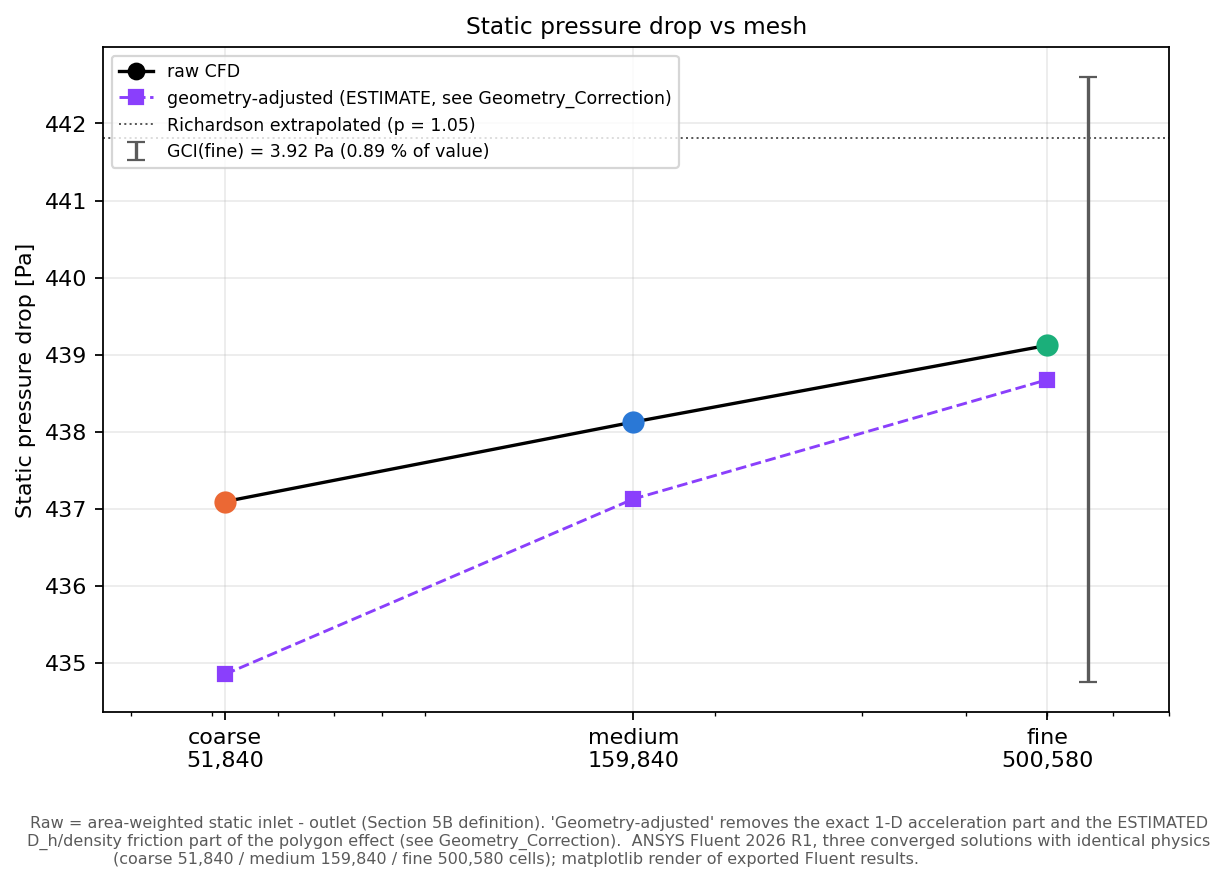
\includegraphics[width=\linewidth,height=52mm,keepaspectratio]{MI01_cells_vs_pressure_drop.png}\caption{Pressure drop [Pa]}\end{subfigure}\hfill
\begin{subfigure}[t]{0.49\linewidth}\centering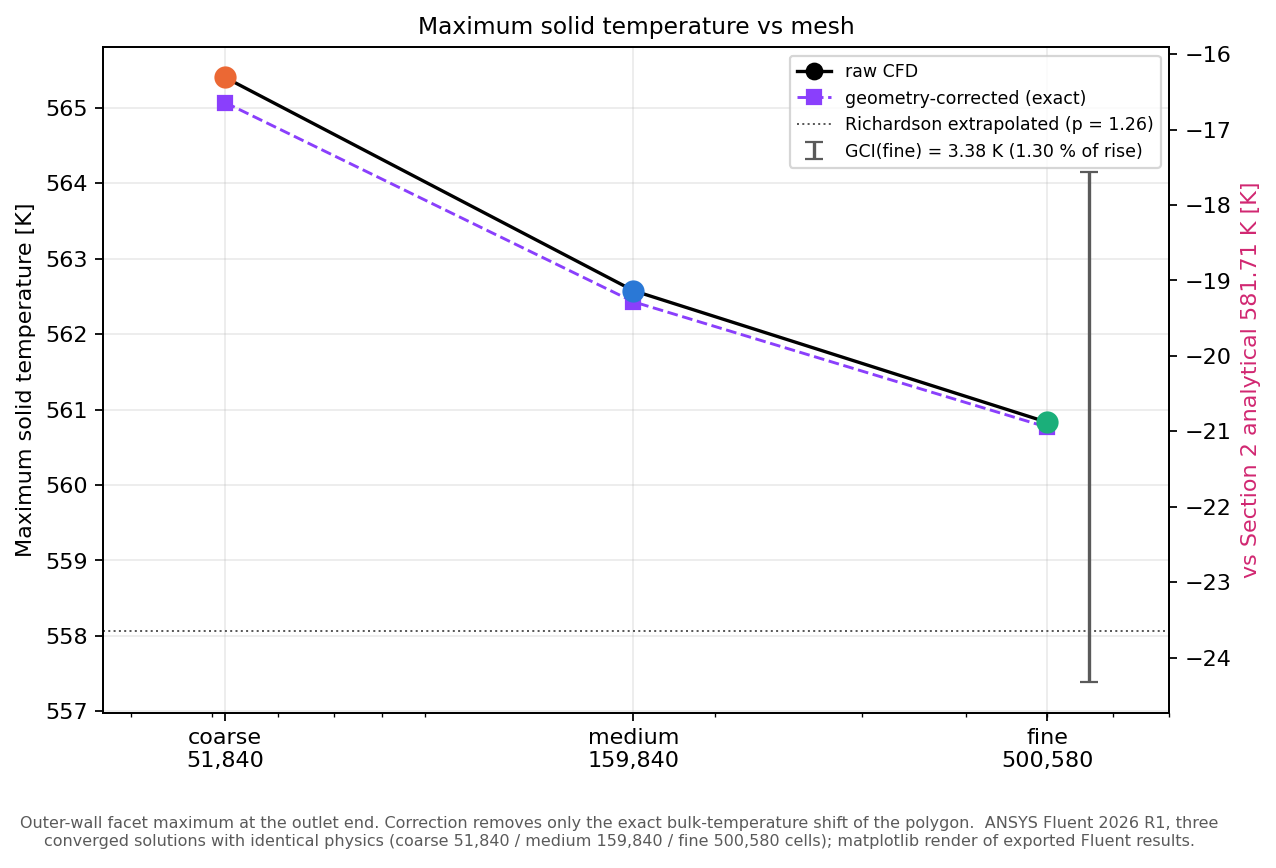
\includegraphics[width=\linewidth,height=52mm,keepaspectratio]{MI04_cells_vs_max_solid_temperature.png}\caption{Maximum solid temperature [K]}\end{subfigure}\\[4pt]
\begin{subfigure}[t]{0.49\linewidth}\centering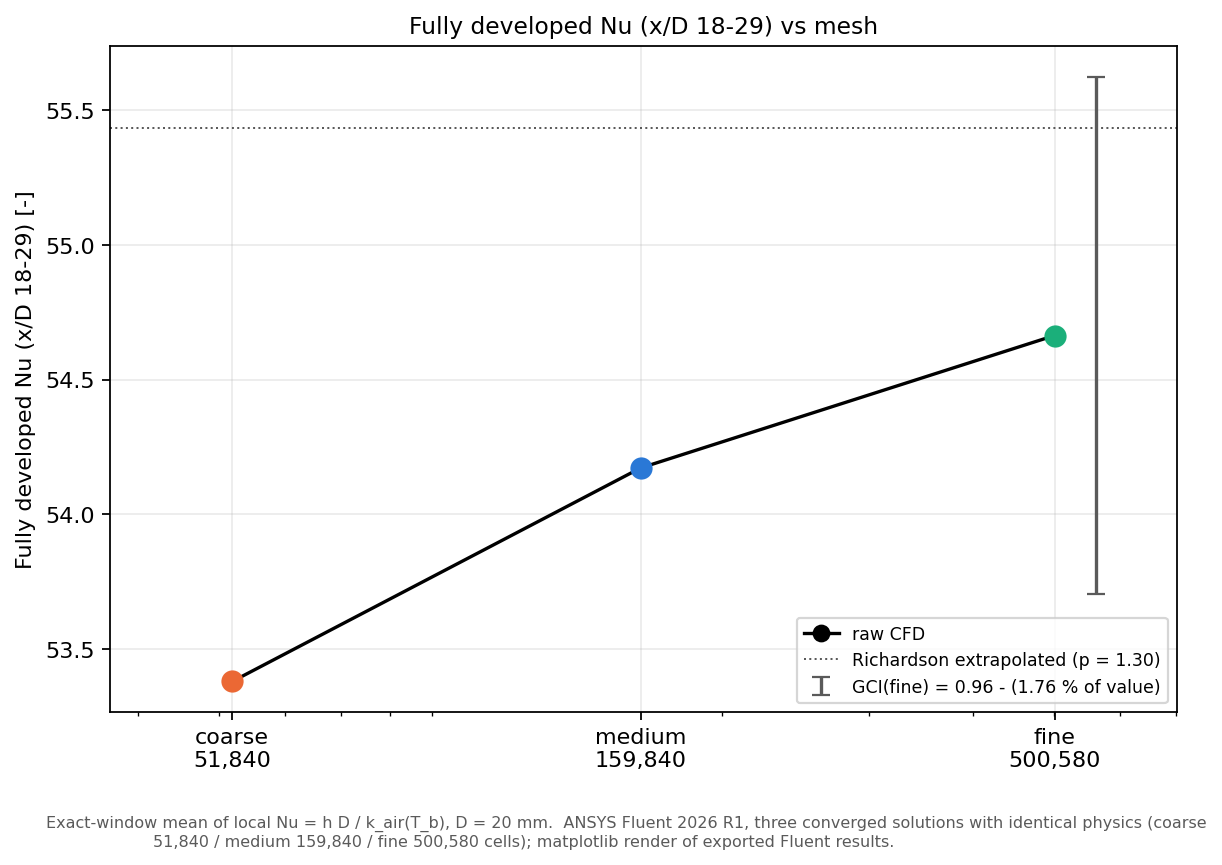
\includegraphics[width=\linewidth,height=52mm,keepaspectratio]{MI06_cells_vs_nusselt.png}\caption{Fully developed Nusselt number}\end{subfigure}\hfill
\begin{subfigure}[t]{0.49\linewidth}\centering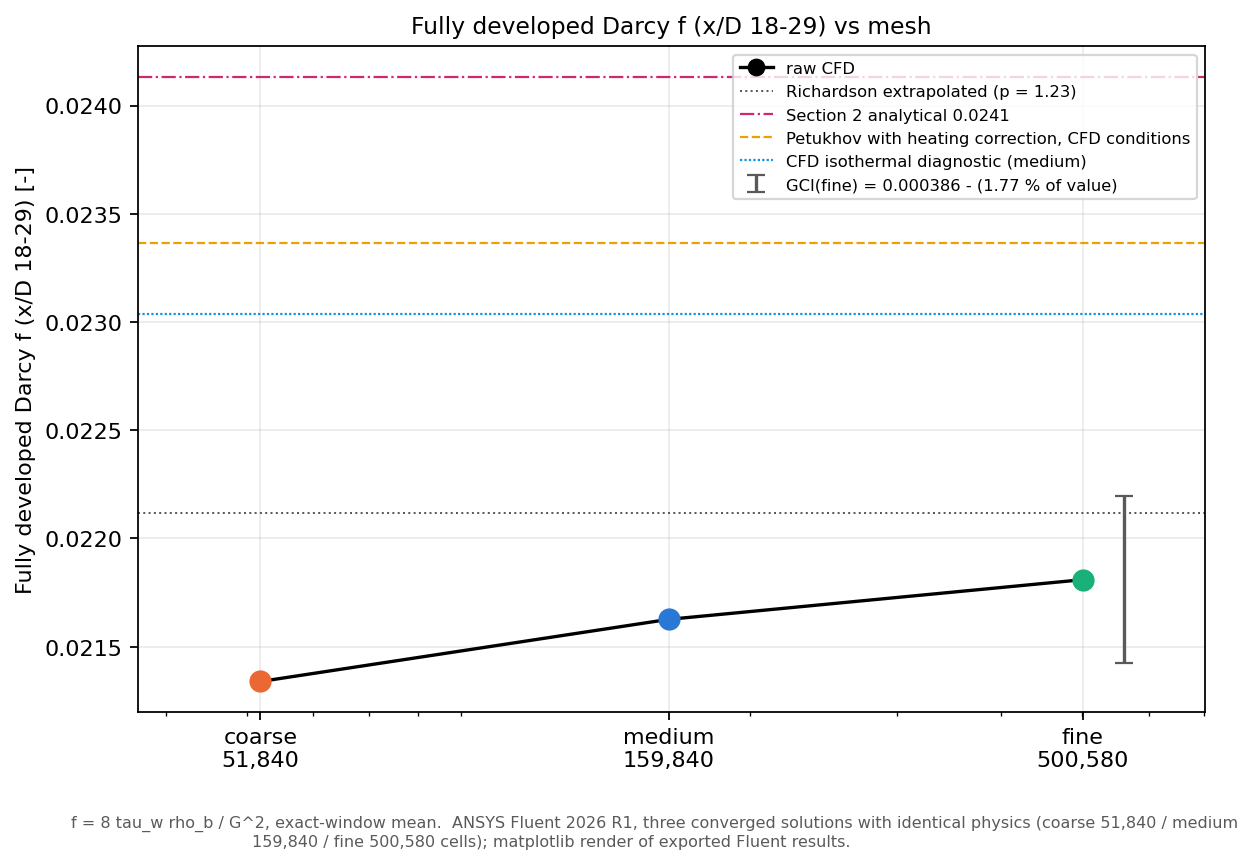
\includegraphics[width=\linewidth,height=52mm,keepaspectratio]{MI07_cells_vs_friction_factor.png}\caption{Fully developed Darcy friction factor}\end{subfigure}
\caption[Mesh-independence study]{Mesh-independence study: raw CFD results on the three meshes, geometry-adjusted values, Richardson extrapolation and GCI$_{fine}$ error bars.}
\label{fig:mi}
\src{\provcfd{} In (b) the extrapolated line belongs to the bulk-corrected series ($p$ = 1.26, 558.06~K); the raw series gives $p$ = 1.31 and 558.13~K (Table~\ref{tab:gci}).}
\end{figure}

\section{Geometry/Faceting Effect}
The three meshes approximate the circular sections by inscribed polygons with 32, 48 and 72 sides. The flow area, heated area and therefore
the mass flow, heat input and outlet temperature change with the number of sides by exactly known ratios. These changes are geometry, not
discretisation error, and were separated exactly before any convergence assessment (decision D-035). Corrected to the true circle, the mass
flow is 8.68694~g/s and the heat input 603.186~W on all three meshes; Richardson extrapolation of the raw values recovers the exact circle
values to within 0.004\,\%, which checks the procedure. Of the raw changes, nearly all of those in mass flow, heat rate and outlet temperature are geometric,
only 5--7\,\% of the change in maximum solid temperature, and a negligible part of the changes in Nusselt number and friction factor.


\section{Pressure-Drop Convergence}
The raw pressure drop increases monotonically (437.09, 438.13, 439.12~Pa), but the geometric part of the change opposes the resolution trend,
so the raw values give no credible order. The geometry-adjusted estimate has an apparent order of 1.05 and extrapolates to 441.8~Pa with a
fine-mesh GCI of 0.89\,\% (3.9~Pa). The medium value is 0.8\,\% below that estimate.

\section{Thermal Convergence}
The maximum solid temperature decreases monotonically (565.40, 562.58, 560.83~K) with an apparent order of 1.31, extrapolating to 558.13~K
with GCI$_{fine}$ = 3.4~K, 1.3\,\% of the temperature rise (Table~\ref{tab:gci}). Refinement raises the heat-transfer coefficient slightly
and therefore lowers the wall temperature, which moves the CFD further from the analytical 581.71~K. The mid-span through-wall temperature
difference converges to 7.620~K with GCI$_{fine}$ = 0.029~K.

%% generated by gen_tables.py - RE-ANALYSIS 2026
\begin{table}[htbp]
\centering
\footnotesize
\caption{Convergence indicators (Celik et al.\ procedure, $r_{21}$ = 1.4631, $r_{32}$ = 1.4555)}
\label{tab:gci}
\begin{tabular}{lrrrr}
\toprule
Quantity & Ratio $R$ & Apparent order $p$ & Extrapolated & GCI$_{fine}$ \\
\midrule
$\Delta p$, geometry-adjusted & 0.68 & 1.05 & 441.8 Pa & 0.89\,\% (3.9 Pa) \\
$T_{max}$ solid & 0.62 & 1.31 & 558.1 K & 3.4 K (1.3\,\% of rise) \\
$\Delta T_{wall}$ mid-span & 0.60 & 1.37 & 7.620 K & 0.029 K \\
$Nu_{fd}$ & 0.62 & 1.30 & 55.43 & 1.8\,\% \\
$f_{fd}$ & 0.64 & 1.23 & 0.02212 & 1.8\,\% \\
\bottomrule
\end{tabular}
\par\smallskip\parbox{\linewidth}{\footnotesize\raggedright Source: \texttt{PROJECT\_STATE.md} \S12.4 and \texttt{09\_Mesh\_Independence/Mesh\_Independence\_Report.md} \cite{celik2008}. Convergence is monotonic but the apparent order is below the formal value of 2.}
\end{table}


\section{Nusselt Number Convergence}
The fully developed Nusselt number increases monotonically (53.38, 54.17, 54.66) with an apparent order of 1.30 and extrapolates to 55.43
(GCI 1.8\,\%). Every value lies inside the expected band of 44--67. Convergence is monotonic for all quantities, but the apparent orders of
1.2--1.6 are below the formal second order, because the first layer is identical on all meshes and the directional refinement ratios are not
equal. The status of every flow and thermal quantity is therefore ``approximately convergent''; strict mesh independence is not claimed.

\section{Friction-Factor Behavior}
The friction factor rises with refinement (0.02134, 0.02163, 0.02181) towards an extrapolated 0.02212, still 8.4\,\% below the Petukhov
value. An isothermal diagnostic run on the medium mesh (energy equation off) gives $f$ = 0.02304, only 2.6\,\% below Petukhov
(Figure~\ref{fig:mifric}). The medium-mesh gap of $-$10.4\,\% decomposes exactly into a Reynolds-number basis factor of 1.011, an isothermal SST
factor of 0.974 and a heating factor of 0.910. The difference is therefore mainly a gas-heating (variable-property) effect, not a mesh defect;
about five percentage points remain unexplained by the standard $(T_w/T_b)^{-0.1}$ heating correction (finding F-034).

\begin{figure}[htbp]
\centering
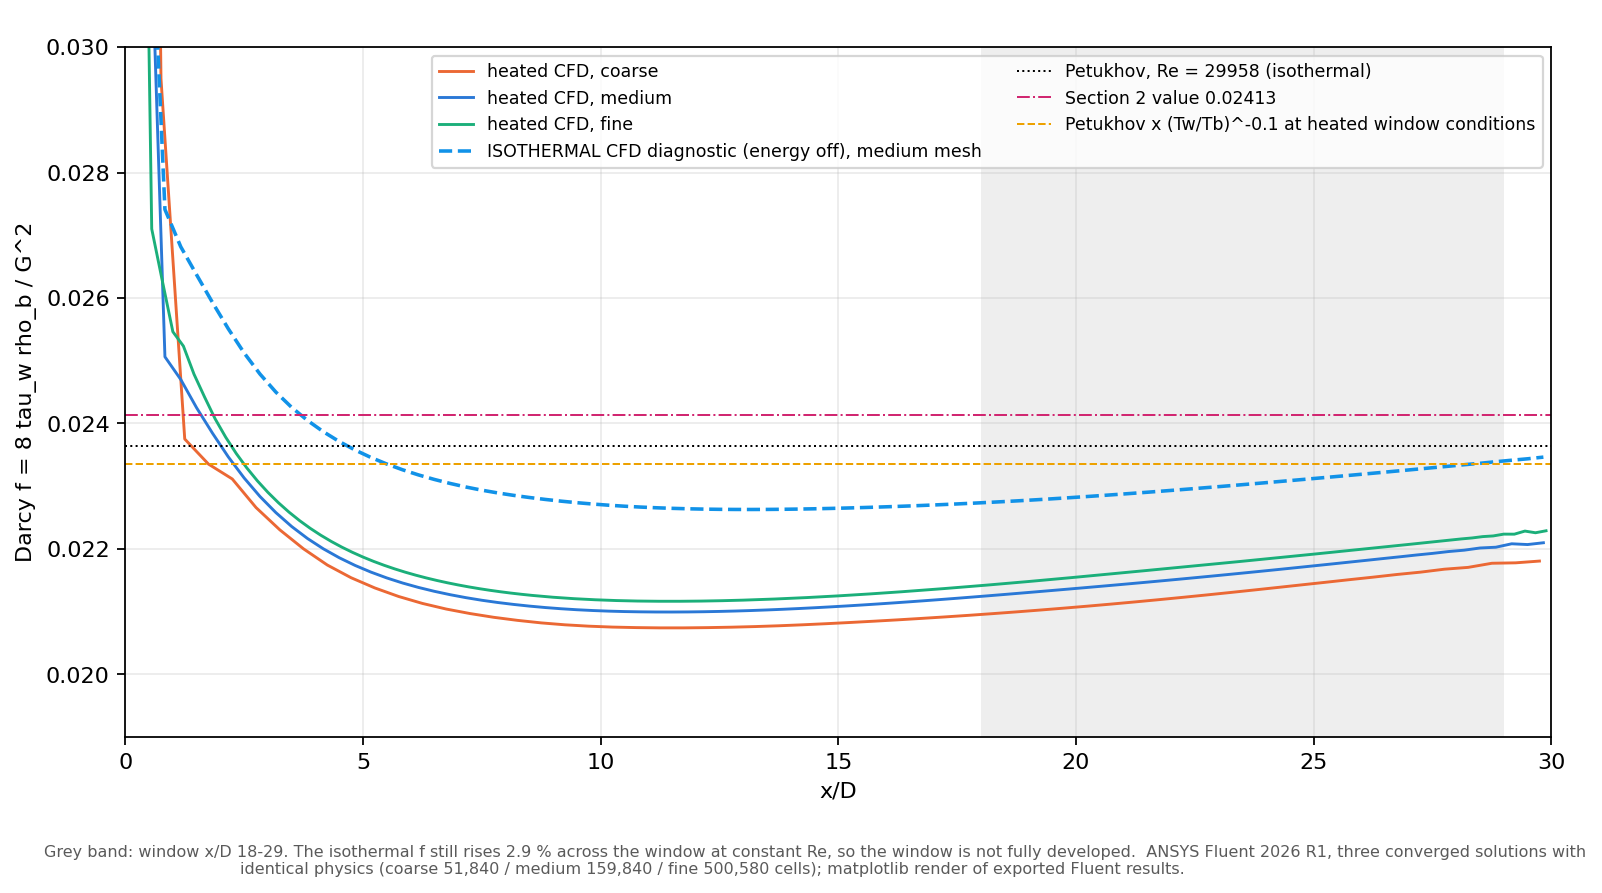
\includegraphics[width=0.68\linewidth]{MI11_F029_friction_evidence_nt.png}
\caption{Local Darcy friction factor on the three heated meshes and in the isothermal diagnostic, compared with Petukhov with and without the heating correction.}
\label{fig:mifric}
\src{\provcfd}
\end{figure}

\section{Final Mesh Selection}
The medium mesh was retained for all downstream work, with the fine mesh as the verification reference (D-034). The reasons are:
\begin{itemize}
\item its error is small and conservative for thermal stress and growth (maximum solid temperature +4.4~K, volume mean +3.1~K above the extrapolated values);
\item the mesh error is about one quarter of the 19~K difference between the CFD and the analytical model, so the dominant thermal uncertainty is the
      heat-transfer and friction modelling, which a finer mesh does not reduce;
\item the fine mesh costs 3.4 times the run time and 4 times the storage;
\item the medium solid fits a 1:1 structural mesh under the 128,000-node Student limit, whereas the fine solid would not.
\end{itemize}
The structural consequence of the mesh error was carried forward as an uncertainty band: LC2 stress $-$10.1 / +2.8~MPa, local peak
$-$13.7 / +4.3~MPa and $\lambda_1$ +1.8 / $-$0.5\,\% (Chapter~\ref{ch:unc}).

% ===================================================================== Chapter 10
\chapter{Thermal Field Transfer}\label{ch:mapping}

\section{CFD-to-Mechanical Workflow}
The converged medium-mesh solution was transferred to ANSYS Mechanical without re-solving any thermal problem: the Fluent solid temperature
field is imported directly into Static Structural as a body temperature (decision D-039). The source case and data files were hash-verified
before and after every structural run and are unchanged. Nineteen read-back checks confirmed that the source is the converged second-order
solution with the correct solid material and a temperature range inside the property tables.

\section{One-Way Coupling}
The coupling is one-way: CFD temperature to structure, with no feedback of deformation to the flow. The analytical thermal growth of the bore radius,
34.94~\textmu m, changes the flow area by only 0.70\,\%, so the flow field is not affected by the deformation. A two-way or fluid--structure interaction analysis would not change the conclusions and was not performed.

\section{Temperature Mapping}
The first method tried, an External Data point cloud of cell and face centroids with triangulation, failed validation: it flagged 77,088
of the 111,216~nodes of the structural mesh then in use as outside the cloud, left 27,696~nodes without a temperature and produced errors of up to 4.0~K. Kriging and
radial-basis interpolation failed in batch mode, and a Workbench Fluent-system route held only the initial 300~K field. These attempts are
kept as evidence. The accepted method is mesh-based External Data:
\begin{itemize}
\item the master mesh is the Fluent solid mesh itself, rebuilt from the case file as an MAPDL archive;
\item the data are Fluent's own node temperatures (48,048~nodes), exported in EnSight format and keyed by node number;
\item Mechanical maps them with the Bucket Volume search and Shape Function interpolation; the outside option is Nearest Node.
\end{itemize}
The 9,408 structural nodes on the outer surface that lie in the 0.038~mm chord gap between the true circle and the 48-sided CFD polygon
receive shape-function values of the adjacent source element (verified), not a nearest-node copy.

\section{Mapping Validation}
Table~\ref{tab:mapping} and Figures~\ref{fig:mapside}--\ref{fig:mapaxial} summarise the checks of the transfer; ``validation'' here means a numerical comparison with the Fluent source field and an
independent reference, not an experimental validation. All 108,252 structural nodes received a
temperature; the mapped range, 423.84--562.56~K, matches the source node range of 423.84--562.54~K. The mid-span through-wall temperature
difference (7.580~K mapped against 7.581~K in Fluent) and the volume mean (525.520~K against 525.483~K) are preserved. In Mechanical the imported field is displayed
in degrees Celsius, 150.69--289.41\,\textdegree C.

%% generated by gen_tables.py - RE-ANALYSIS 2026
\begin{table}[htbp]
\centering
\footnotesize
\caption{Numerical checks of the CFD-to-Mechanical temperature transfer (Section 7A)}
\label{tab:mapping}
\begin{tabular}{>{\raggedright\arraybackslash}p{0.42\linewidth}>{\raggedright\arraybackslash}p{0.48\linewidth}}
\toprule
Check & Result \\
\midrule
Source field & converged medium solution; Fluent node temperatures 423.84--562.54 K (48,048 nodes) \\
Coverage & 108,252 / 108,252 structural nodes mapped; 0 unmapped \\
Mapped range & 423.84--562.56 K (identical in LC1 and LC2) \\
Error (A) against exact shape-function evaluation & maximum 0.081 K inside the source mesh; mean 0.002 K \\
Error (B) against independent finite-volume reference & maximum 2.57 K at the bore within $\sim$11 mm of the inlet; $\le$ 0.25 K over $z$ = 14--586 mm; mean 0.039 K \\
Mid-span through-wall $\Delta T$ & mapped 7.580 K against Fluent 7.581 K \\
Volume-mean temperature & mapped 525.520 K against Fluent 525.483 K \\
Parametric cases (9B-2) & all 7 cases passed; error (A) 0.086--0.154 K \\
\bottomrule
\end{tabular}
\par\smallskip\parbox{\linewidth}{\footnotesize\raggedright Source: \texttt{07\_Thermal\_Analysis/THERMAL\_MAPPING\_NOTES.md}, \texttt{CFD\_TO\_MECHANICAL\_MAPPING\_AUDIT.md}, \texttt{PROJECT\_STATE.md} \S13.1 and \S19.2.}
\end{table}


\begin{figure}[htbp]
\centering
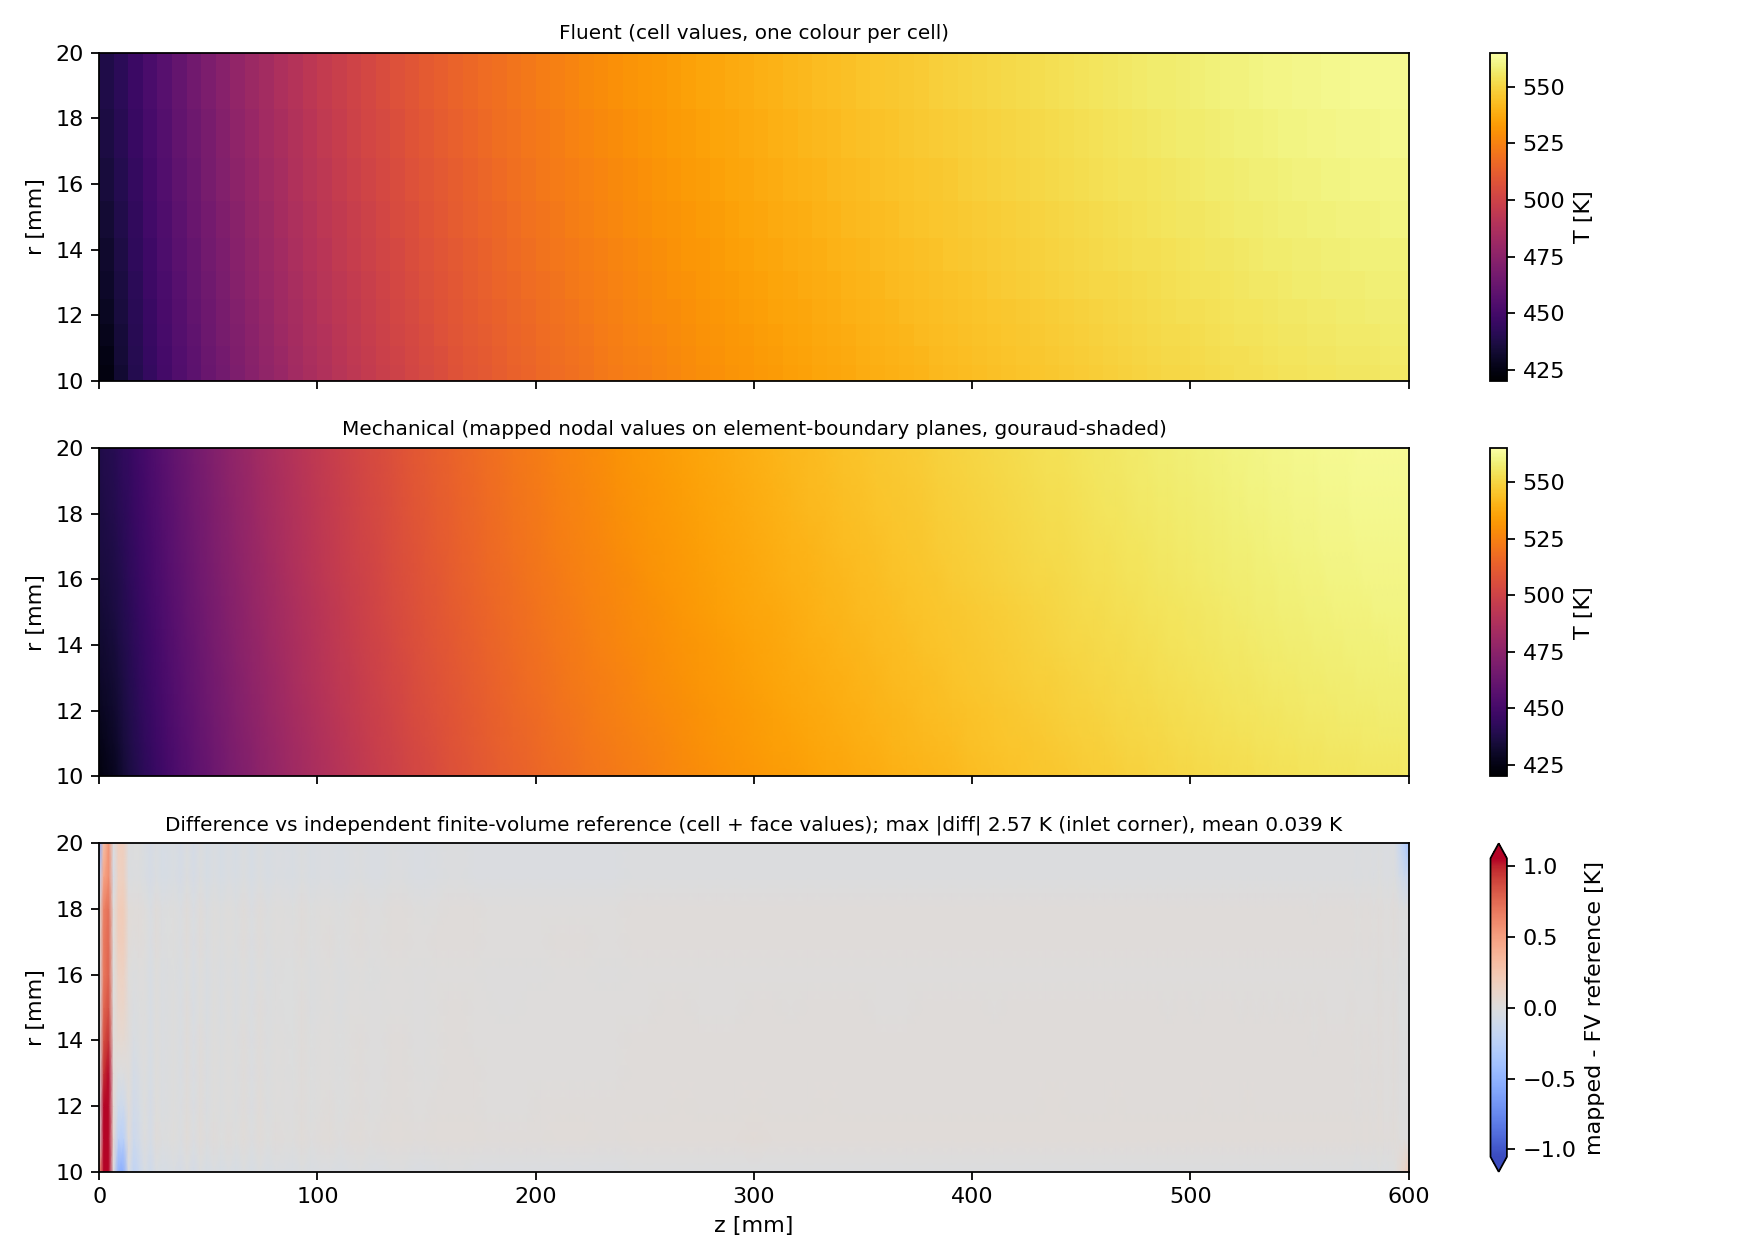
\includegraphics[width=0.68\linewidth]{F7A_03_side_by_side_and_difference_nt.png}
\caption{Fluent source temperature (top), temperature mapped onto the Mechanical nodes (middle) and difference from an independent
finite-volume reference (bottom), circumferential means [K].}
\label{fig:mapside}
\src{\provdata}
\end{figure}

\begin{figure}[htbp]
\centering
\begin{subfigure}[t]{0.56\linewidth}\centering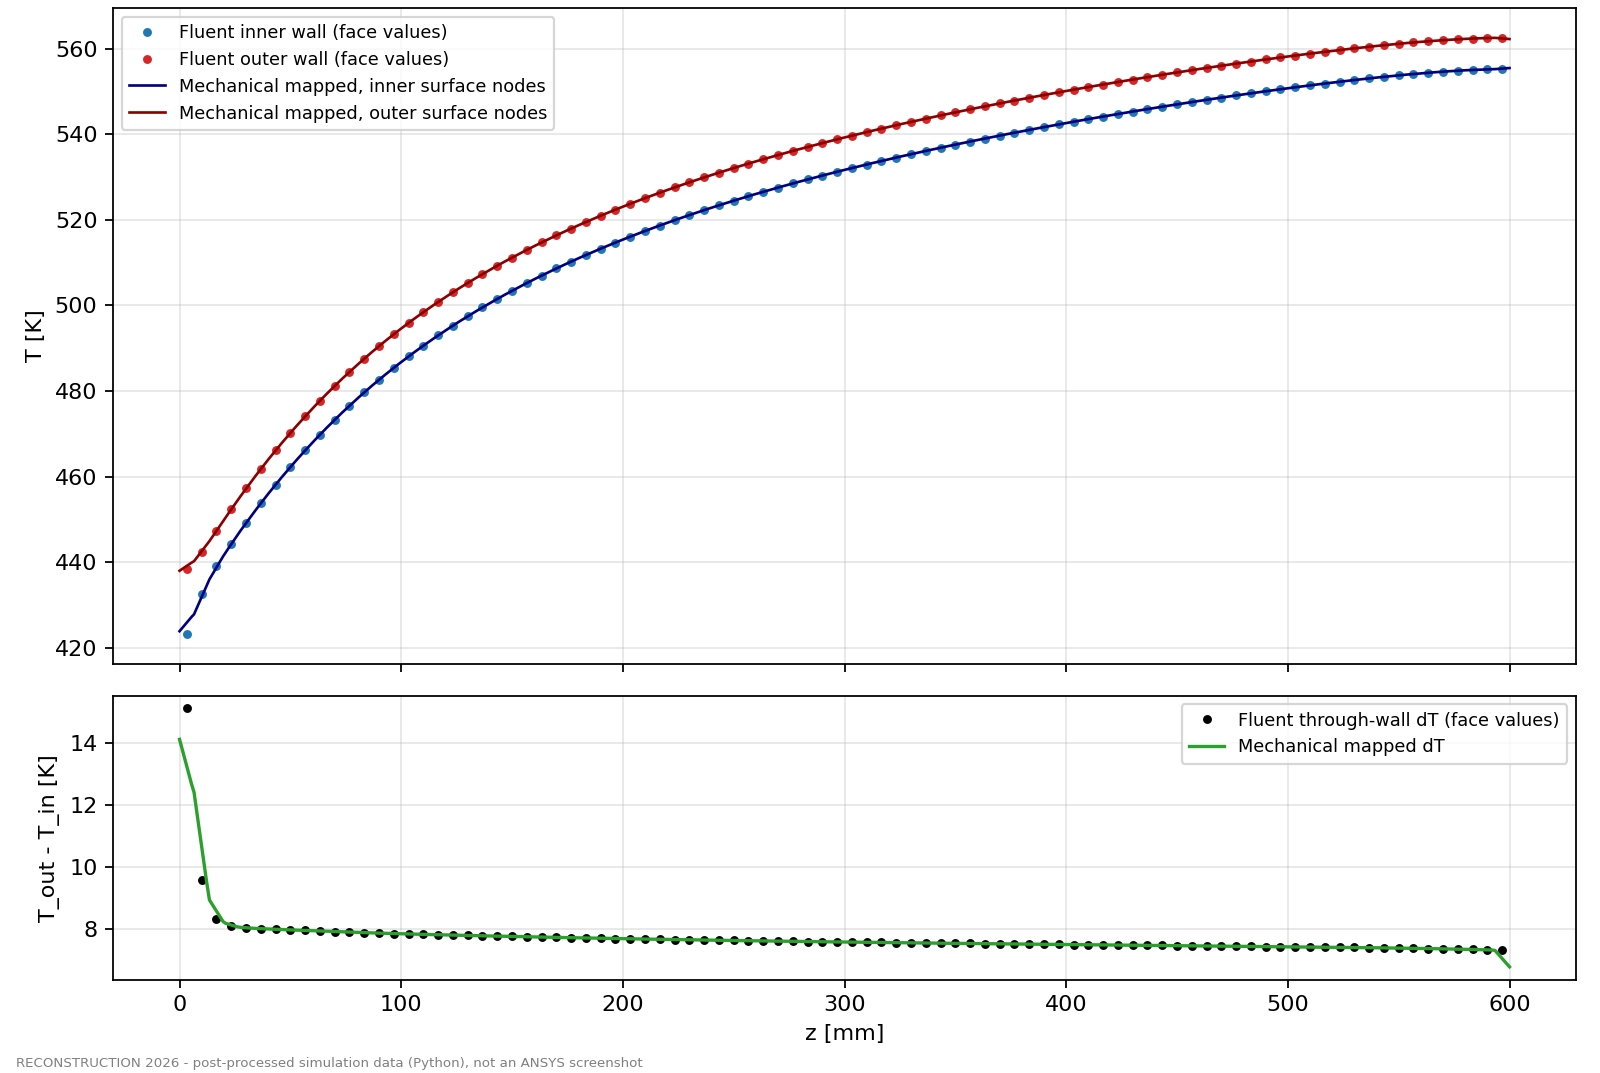
\includegraphics[width=\linewidth,height=52mm,keepaspectratio]{F7A_04_axial_wall_temperature_nt.png}\caption{Inner and outer wall temperature and through-wall $\Delta T$ along the duct}\end{subfigure}\hfill
\begin{subfigure}[t]{0.42\linewidth}\centering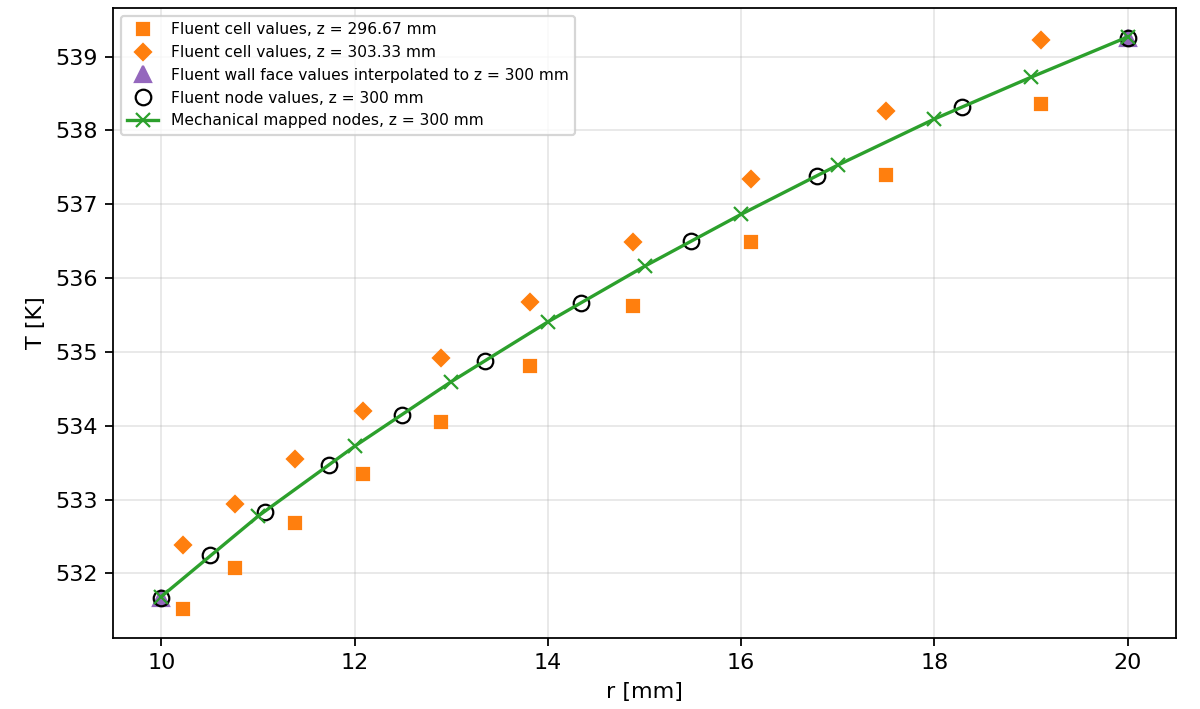
\includegraphics[width=\linewidth,height=52mm,keepaspectratio]{F7A_05_through_wall_midspan_nt.png}\caption{Through-wall profile at mid-span}\end{subfigure}
\caption{Mapped temperatures compared with the Fluent source values.}
\label{fig:mapaxial}
\src{\provdata}
\end{figure}


\section{Mapping Error}
Two error measures are distinguished. Error (A) compares the mapped value with the exact shape-function evaluation of the source node
field: at most 0.081~K inside the source mesh, mean 0.002~K. This is the error of the transfer itself. Error (B) compares the mapped value
with an independent finite-volume reference built from the cell and face values: at most 2.57~K, at the bore within about 11~mm of the inlet,
and at most 0.25~K over $z$ = 14--586~mm. Error (B) reflects Fluent's reconstruction of node values from cell values in the region of the
steepest gradients; it is a property of the source data, identical on every structural mesh. Its effect was bounded at $\pm$9.8~MPa on the
LC1 inlet peak stress and 1.6\,\% on the LC2 peak; interior values are unaffected. Every parametric case was mapped with the same method and
passed the same checks, with error (A) between 0.086 and 0.154~K.

\section{Reference Temperature}
The stress-free reference temperature is $T_{ref}$ = 300~K, equal to the inlet air temperature (decision D-041).
The thermal load is the full spatial field $\Delta T(x,y,z) = T - T_{ref}$, which ranges from 123.8 to 262.6~K; neither the analytical mean
temperature nor the CFD maximum is used as a uniform substitute. The reference value was read back from every solver input file.

\section{Temperature-Dependent Material Properties}
The structural material uses $E(T)$ from the VDM table (204~GPa at 20\,\textdegree C to 180~GPa at 400\,\textdegree C) and the secant $\alpha(T)$
from 12.8 to $14.8\times10^{-6}$/K, re-referenced by the solver from the 70\,\textdegree F datum of the data to $T_{ref}$. Every node lies
inside the tabulated temperature range, so no property is extrapolated. $S_y(T)$ is interpolated at the node temperature only for the yield
assessment.

% ===================================================================== Chapter 11
\chapter{Thermo-Structural Analysis}\label{ch:struct}

\section{Structural Model}
The structural model (Table~\ref{tab:smodel}) is a linear static ANSYS Mechanical \cite{ansysmech} model of the Inconel 718 annulus loaded only by the mapped
temperature field. Before any solve, a gate of 61 automated checks compared the written solver inputs with the prepared model section by
section (nodes, elements, temperatures, material, constraints). Each load case solved in about one minute with the sparse direct solver.

%% generated by gen_tables.py - RE-ANALYSIS 2026
\begin{table}[htbp]
\centering
\footnotesize
\caption{Structural model of the baseline (Section 7B)}
\label{tab:smodel}
\begin{tabular}{>{\raggedright\arraybackslash}p{0.30\linewidth}>{\raggedright\arraybackslash}p{0.60\linewidth}}
\toprule
Item & Setting \\
\midrule
Software & ANSYS Mechanical / MAPDL 2026 R1 (Student licence, measured limit 128,000 nodes) \\
Mesh B & SOLID186 quadratic hexahedra, 36 circumferential $\times$ 5 through-wall $\times$ 130 axial (bias 4, 2.13 $\rightarrow$ 8.51 mm); 108,252 nodes / 23,400 elements \\
Element quality & minimum 0.237 (average 0.688); aspect ratio $\le$ 4.88; Jacobian ratio $\le$ 1.205 \\
Thermal load & mapped CFD solid temperature on every node; $\Delta T = T(x,y,z) - T_{ref}$ \\
Reference temperature & 300 K \\
Material & $E(T)$, secant $\alpha(T)$, $\nu$ = 0.294 [ASSUMED]; $S_y(T)$ used only for assessment \\
Analysis & linear static, small deflection, sparse direct solver \\
Load cases & LC1 (free expansion), LC2 (axially restrained, S1), LC2P (LC2 + 443.41 Pa bore pressure) \\
\bottomrule
\end{tabular}
\par\smallskip\parbox{\linewidth}{\footnotesize\raggedright Source: \texttt{MASTER\_PROJECT\_DATA.csv} rows M081--M083; \texttt{PROJECT\_STATE.md} \S13.1 and \S14.1.}
\end{table}


\section{Structural Mesh}
Mesh B uses quadratic 20-node hexahedra (SOLID186), five through the wall (2.0~mm each), 36 around the circumference and 130 along the axis,
graded towards the inlet where the temperature gradients are largest (Figure~\ref{fig:smesh}). With 108,252~nodes it uses 84.6\,\% of the
measured Student limit. Its adequacy is demonstrated by the seven-mesh study of Chapter~\ref{ch:smesh}.

\begin{figure}[htbp]
\centering
\begin{subfigure}[t]{0.58\linewidth}\centering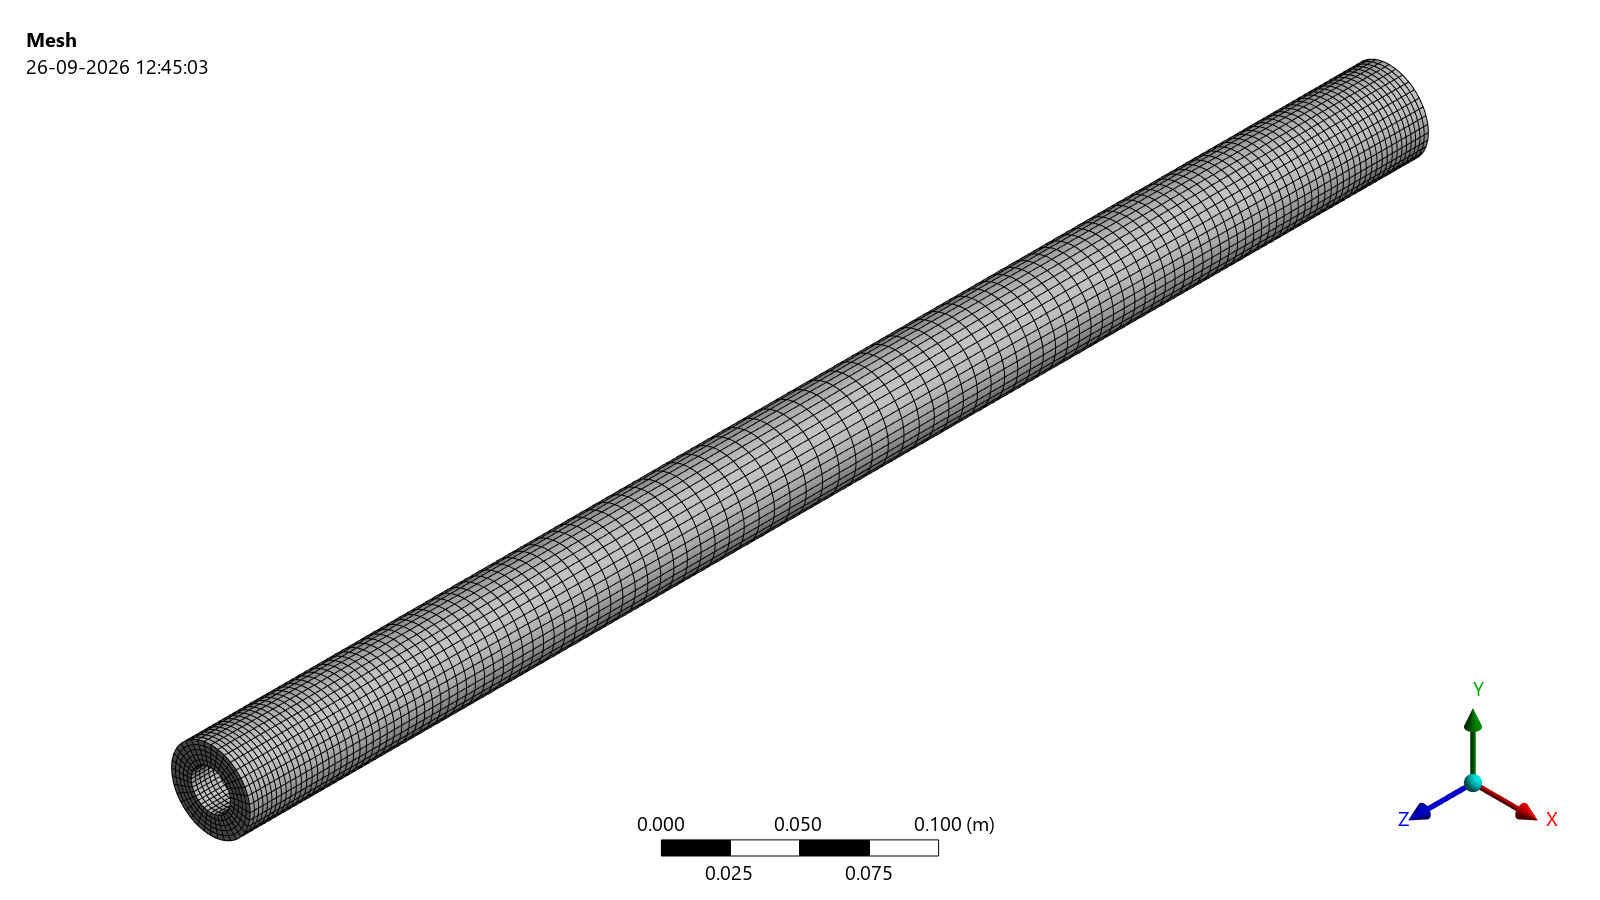
\includegraphics[width=\linewidth,trim=0 80 0 60,clip]{B_mesh_iso.png}\caption{Isometric view}\end{subfigure}\hfill
\begin{subfigure}[t]{0.40\linewidth}\centering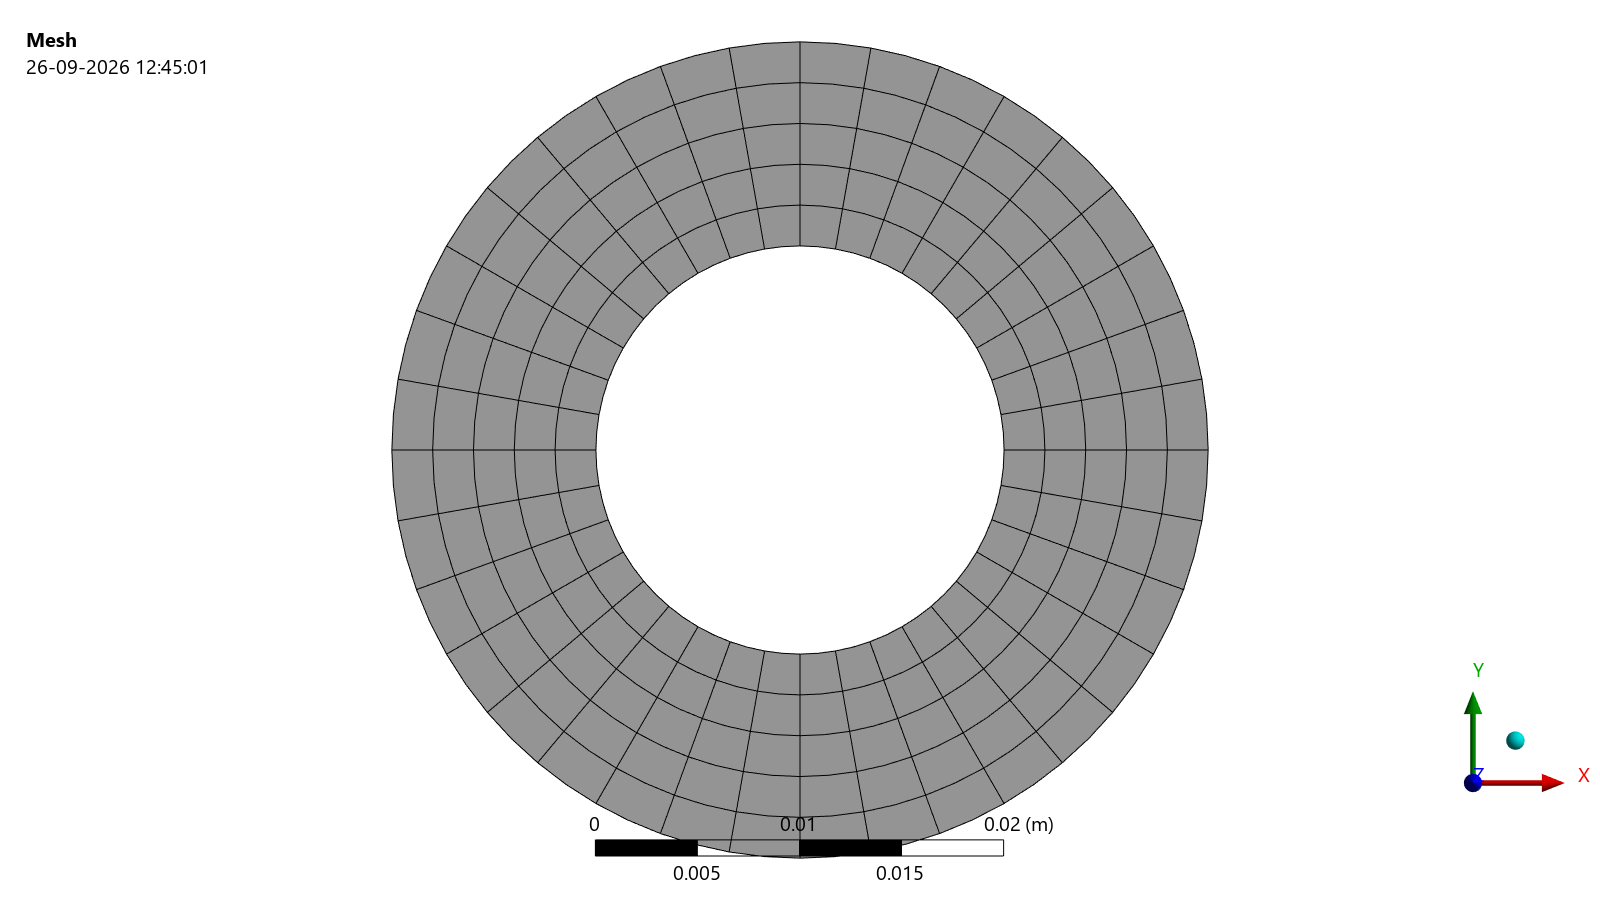
\includegraphics[width=\linewidth,trim=250 40 250 40,clip]{B_mesh_end_face.png}\caption{End face: 36 $\times$ 5 elements}\end{subfigure}
\caption[Structural mesh B]{Structural mesh B: 108,252~nodes, 23,400 SOLID186 elements.}
\label{fig:smesh}
\src{\provmech{} The white margins of the export are trimmed for layout.}
\end{figure}

\section{LC1 Free Expansion}
In LC1 the duct is supported in a statically determinate way and can expand freely; the reactions are about $10^{-6}$ N, confirming that no
spurious restraint exists. The maximum total deformation is 1.8443~mm at the outer edge of the outlet face, and the free axial growth
(area-weighted mean over the end face) is 1.8409~mm (Figure~\ref{fig:lc1}). An independent integration of the thermal strain over the same
temperature field gives the same growth to $1.3\times10^{-5}$. The growth is 12.2\,\% below the Section 2 estimate of 2.096~mm because the CFD mean
temperature rise (about 225.5~K) is lower than the analytical one (254.7~K).

\begin{figure}[htbp]
\centering
\begin{subfigure}[t]{0.49\linewidth}\centering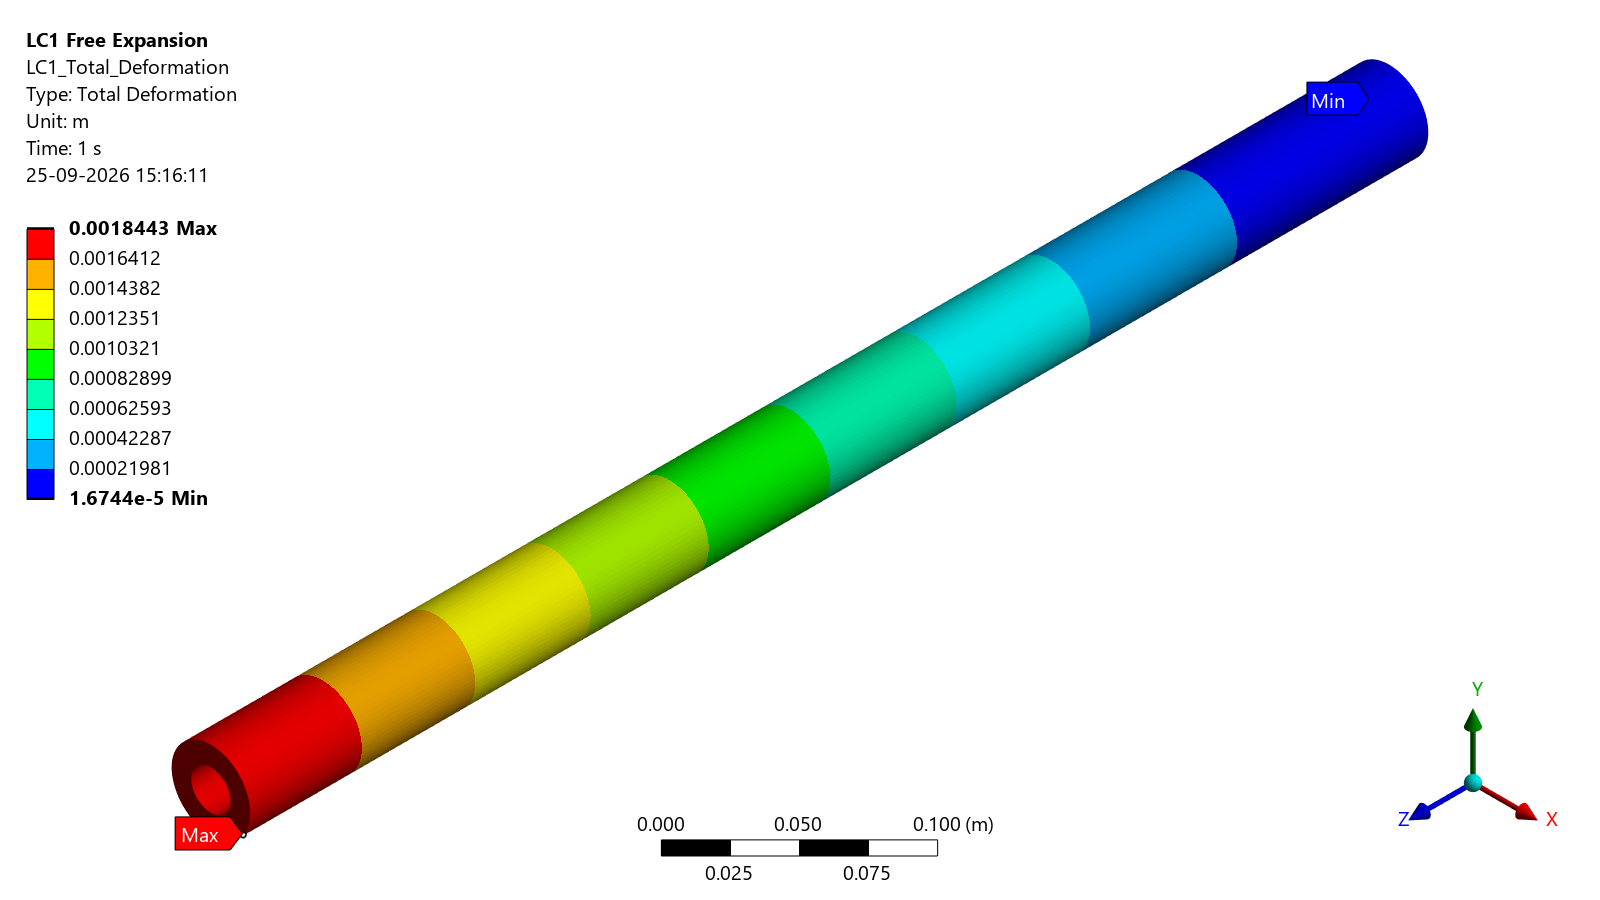
\includegraphics[width=\linewidth,height=52mm,keepaspectratio]{LC1_Total_Deformation_iso.png}\caption{Total deformation [m]}\end{subfigure}\hfill
\begin{subfigure}[t]{0.49\linewidth}\centering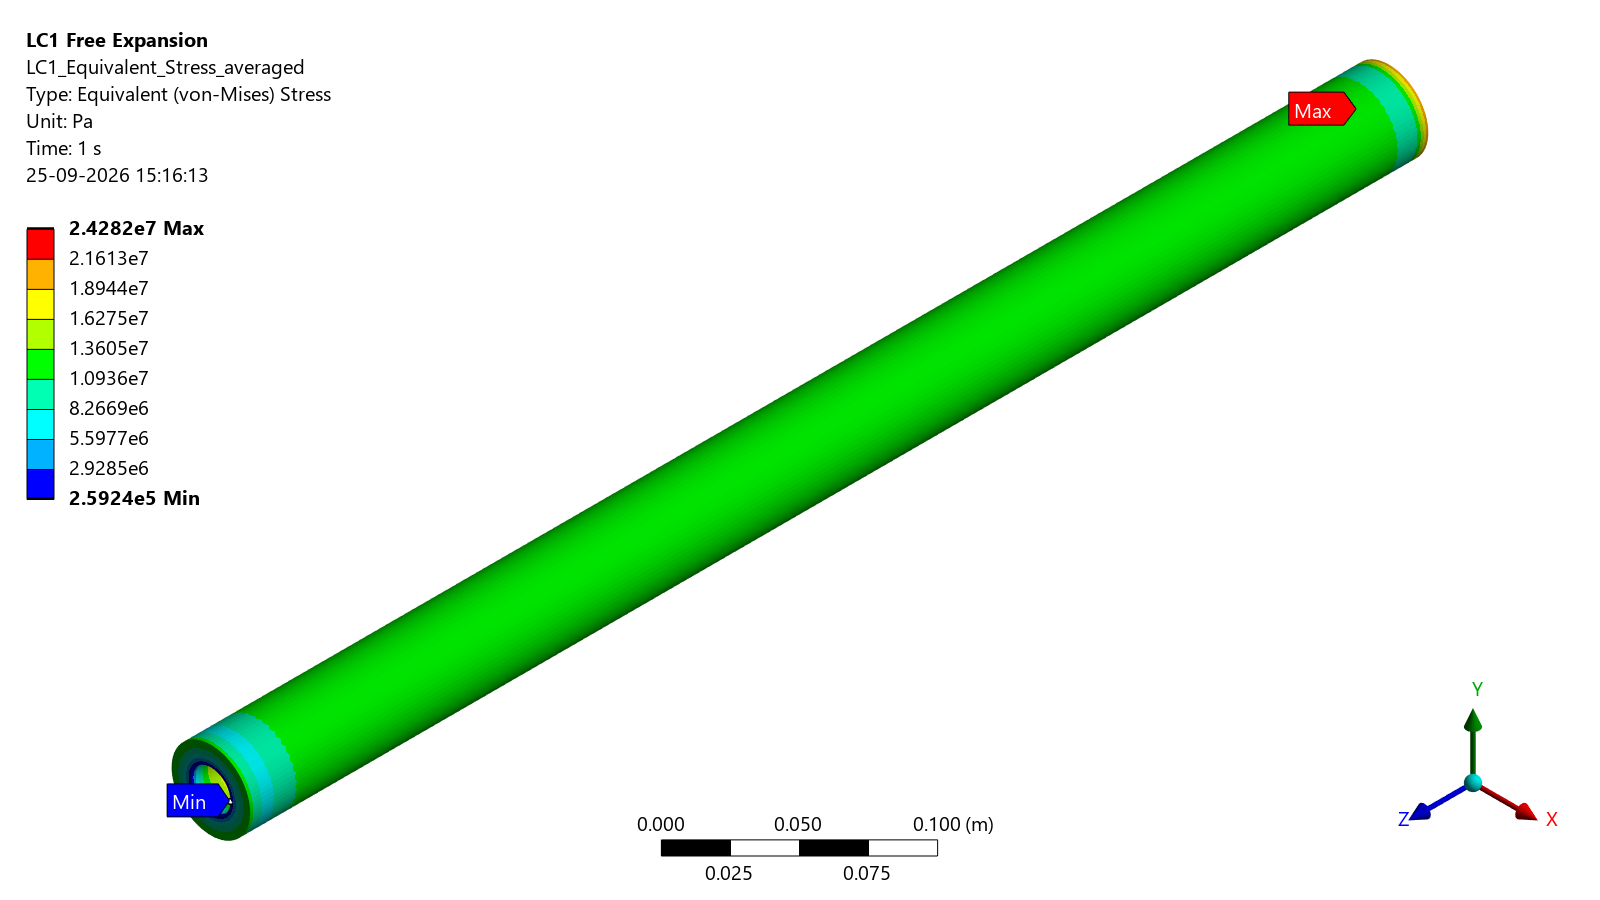
\includegraphics[width=\linewidth,height=52mm,keepaspectratio]{LC1_Equivalent_Stress_averaged_iso.png}\caption{Von Mises stress [Pa]}\end{subfigure}
\caption[LC1 free expansion]{LC1 free expansion: maximum deformation 1.8443~mm at the outlet end; maximum von Mises stress 24.28~MPa at the bore near the inlet.}
\label{fig:lc1}
\src{\provmech}
\end{figure}

The LC1 stresses come only from the non-uniform temperature. Along most of the duct the bore carries about 18~MPa von Mises (18.20~MPa at
mid-span), the value predicted by the thick-cylinder solution, Equation~\eqref{eq:timoshenko}, evaluated on the CFD field (18.55~MPa). The
maximum, 24.28~MPa at the bore 6.5~mm from the inlet face (427.81~K), is an end effect of the steep axial and radial gradients in the first
slab (Figure~\ref{fig:lcprof}a). This peak lies in the region where the mapped temperatures carry the Fluent node-reconstruction limitation,
so its value is bounded at $\pm$9.8~MPa (Chapter~\ref{ch:mapping}); it drives no conclusion.

\section{LC2 Axially Restrained Expansion}
In LC2 both end faces are held axially. The axial growth is prevented, the maximum total deformation drops to 0.1349~mm (outer surface,
$z \approx$ 244~mm), and the duct carries an almost uniform axial compression (Figure~\ref{fig:lc2}). The end faces react $\pm$548,936.6~N,
balanced to $1.8\times10^{-8}$ N and equal to the analytical restrained force of the same temperature field, Equation~\eqref{eq:restrained},
to $10^{-5}$. The mean axial stress is $-$582.44~MPa.

\begin{figure}[htbp]
\centering
\begin{subfigure}[t]{0.49\linewidth}\centering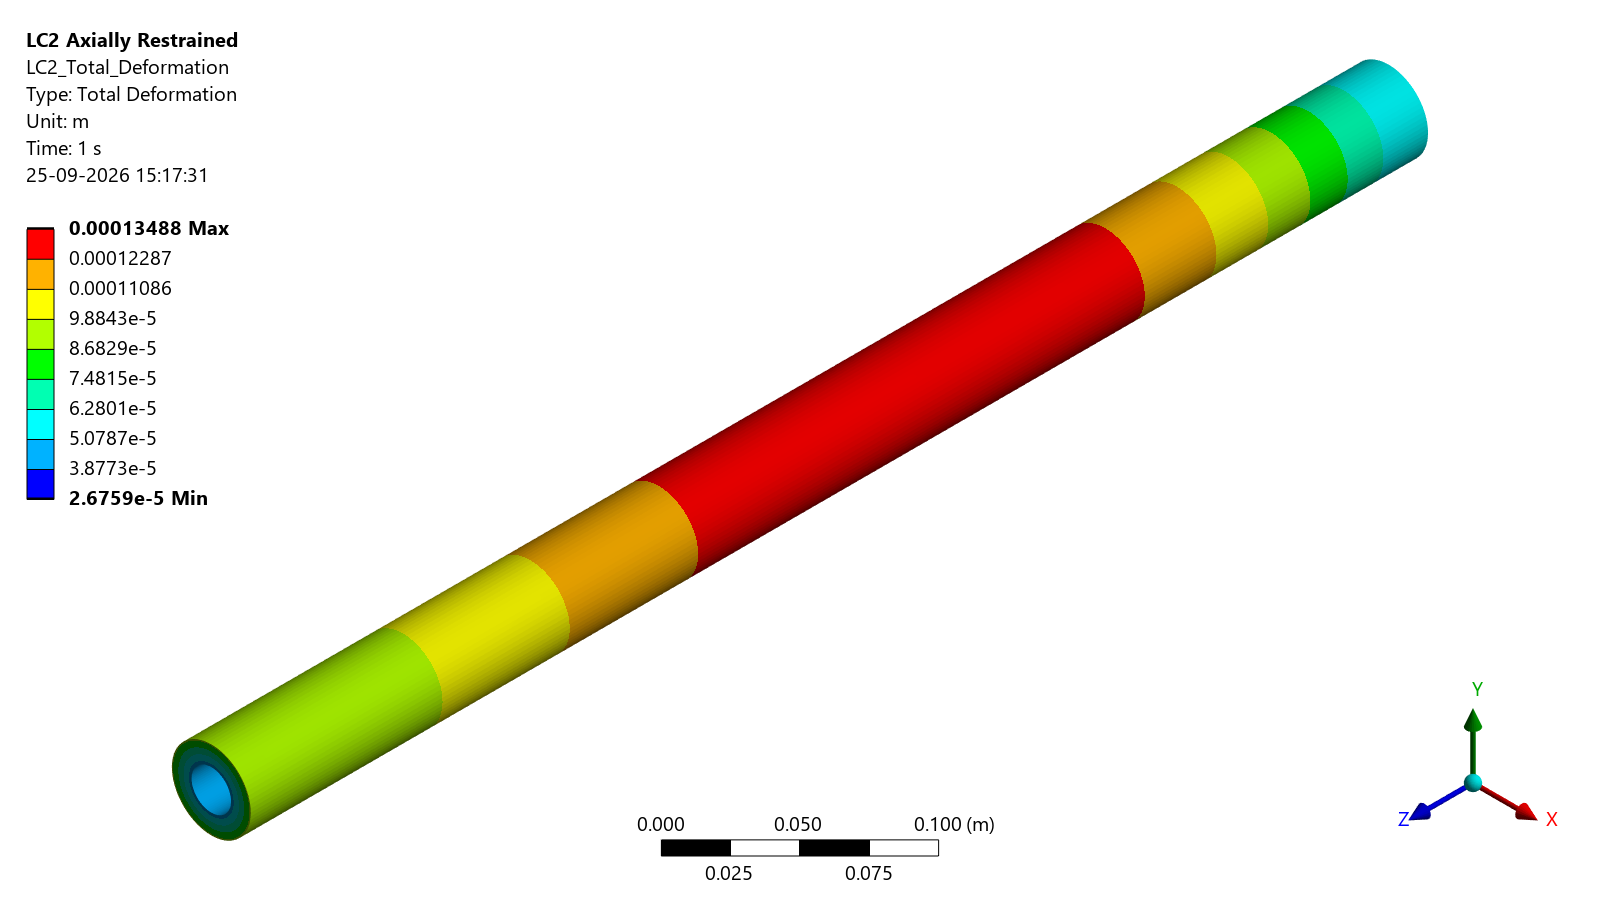
\includegraphics[width=\linewidth,height=52mm,keepaspectratio]{LC2_Total_Deformation_iso.png}\caption{Total deformation [m]}\end{subfigure}\hfill
\begin{subfigure}[t]{0.49\linewidth}\centering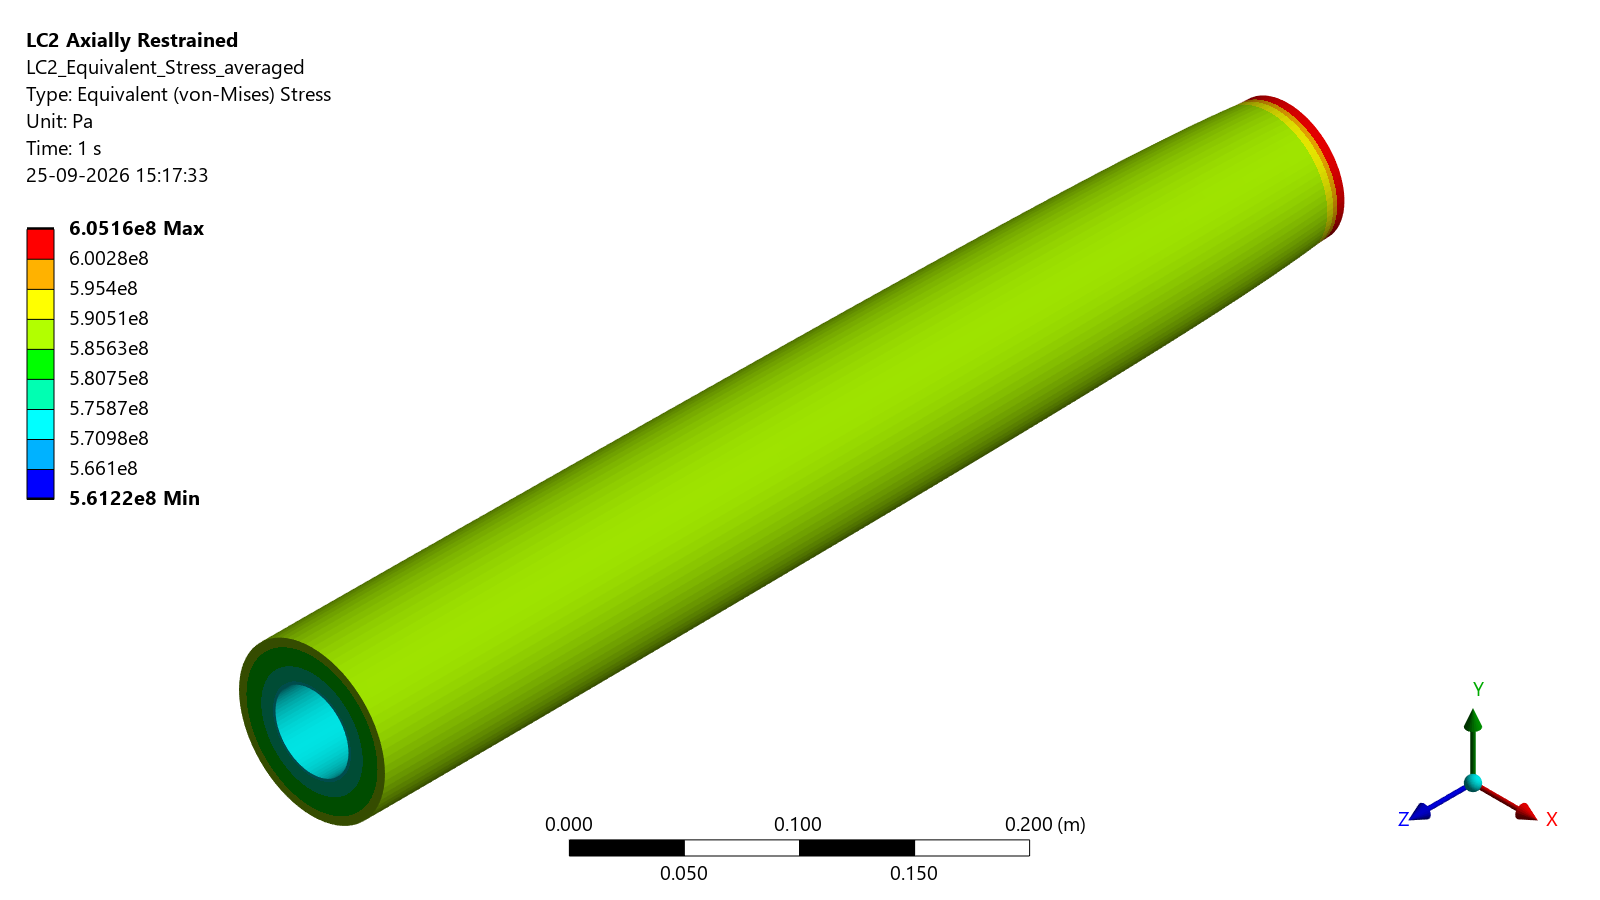
\includegraphics[width=\linewidth,height=52mm,keepaspectratio]{LC2_Equivalent_Stress_averaged_iso.png}\caption{Von Mises stress [Pa]}\end{subfigure}
\caption[LC2 axially restrained expansion (S1 supports)]{LC2 axially restrained expansion (S1 supports): maximum deformation 0.1349~mm; maximum von Mises stress 605.16~MPa at the outer edge of the inlet face.}
\label{fig:lc2}
\src{\provmech}
\end{figure}

\section{Temperature-Dependent Elastic Properties}
Because $E$ decreases and $\alpha$ increases with temperature, the restrained stress $E\alpha\Delta T$ is not proportional to the temperature
rise alone. The analytical model evaluated $E$ and $\alpha$ once at the mean temperature; the FE model evaluates them at every node. Section 2
rescaled to the CFD mean temperature rise gives $-$581.9~MPa, within 0.1\,\% of the FE mean axial stress of $-$582.44~MPa. The difference from
the original analytical $-$657.2~MPa ($-$11.4\,\%) is therefore the temperature basis, not the structural model.

\section{Thermal Stress}
Table~\ref{tab:lcres} summarises both load cases. The LC2 peak von Mises stress of 605.16~MPa occurs at the outer edge of the inlet face
(437.99~K), where the uniform compression combines with the steep temperature gradient of the inlet end (Figure~\ref{fig:lcprof}b). In the interior the von Mises stress is 587--591~MPa, with axial stresses of $-$593.4~MPa at the outer surface and
$-$564.9~MPa at the bore at mid-span. The column load is the end force of 548.94~kN, equivalent to the mean axial
stress of $-$582.44~MPa; the 605.16~MPa is a local peak and not the column load.

%% generated by gen_tables.py - RE-ANALYSIS 2026
\begin{table}[htbp]
\centering
\footnotesize
\caption{Static structural results of the baseline (mesh B)}
\label{tab:lcres}
\begin{tabular}{>{\raggedright\arraybackslash}p{0.42\linewidth}rr}
\toprule
Quantity & LC1 free expansion & LC2 restrained (S1) \\
\midrule
Maximum total deformation [mm] & 1.8443 & 0.1349 \\
Free axial growth $\Delta L$ [mm] & 1.8409 & -- \\
Maximum von Mises stress [MPa] & 24.282 & 605.161 \\
Location of the maximum & bore, $z$ = 6.5 mm & outer edge of the inlet face \\
Temperature at the maximum [K] & 427.81 & 437.99 \\
Mid-span bore von Mises [MPa] & 18.20 & -- \\
Axial end reaction [N] & $\approx 0$ ($9.0\times10^{-7}$) & 548,936.6 \\
Mean axial stress [MPa] & $\approx 0$ & $-$582.440 \\
Pressure effect LC2P $-$ LC2 on the peak [Pa] & -- & +45 \\
\bottomrule
\end{tabular}
\par\smallskip\parbox{\linewidth}{\footnotesize\raggedright Source: \texttt{MASTER\_PROJECT\_DATA.csv} rows M084--M097 (VERIFIED from the MAPDL nodal and reaction tables).}
\end{table}



The ratio of restrained to gradient stress is 32 at mid-span and 25 between the peaks: the axial restraint, not the through-wall temperature
gradient, dominates the thermal stress. This confirms in kind the Section 2 prediction of a factor of about 40.

\begin{figure}[htbp]
\centering
\begin{subfigure}[t]{0.45\linewidth}\centering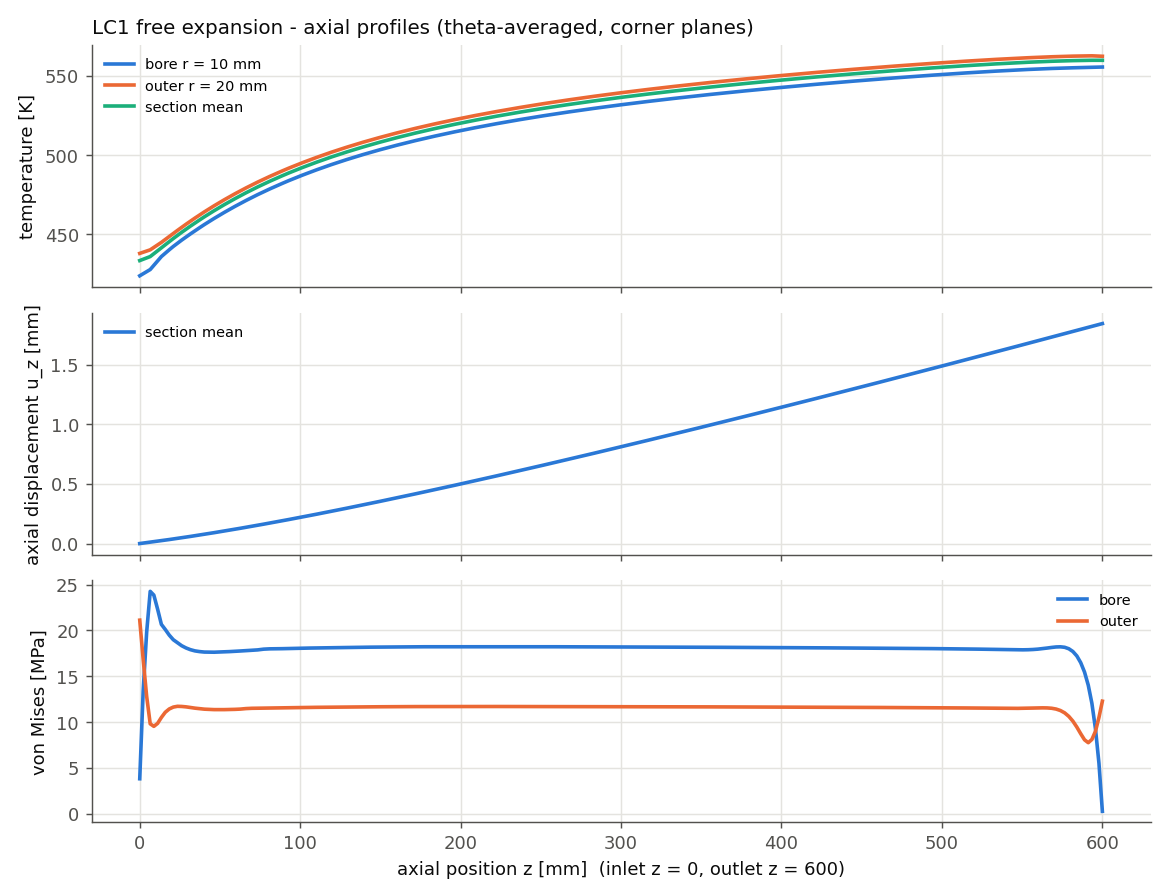
\includegraphics[width=\linewidth,height=78mm,keepaspectratio]{F7B_01_LC1_axial_profiles.png}\caption{LC1: temperature, axial displacement and von Mises stress}\end{subfigure}\hfill
\begin{subfigure}[t]{0.53\linewidth}\centering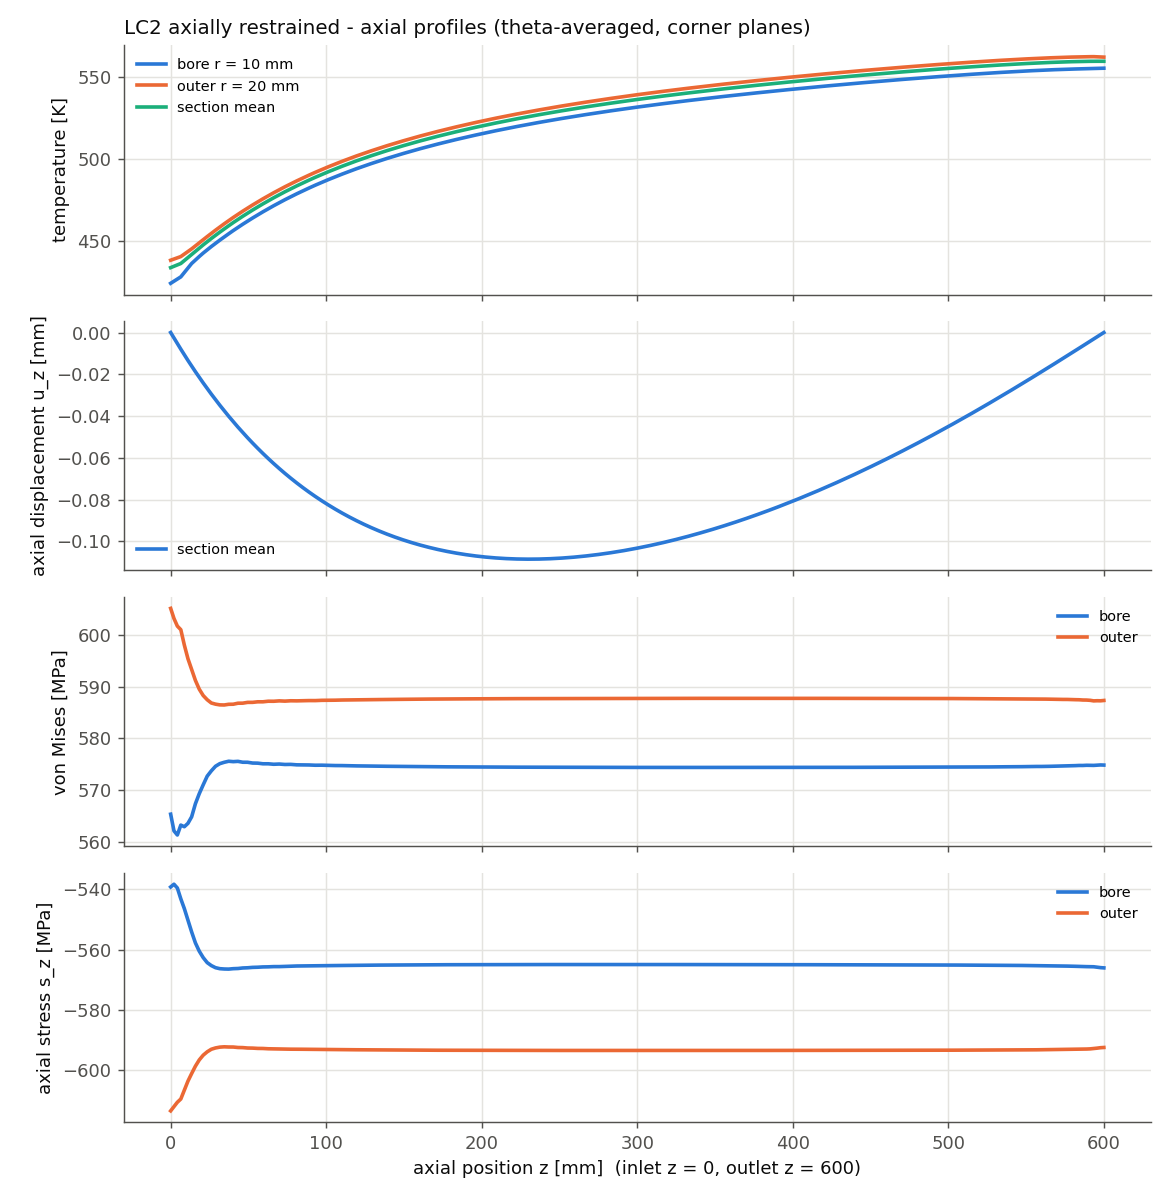
\includegraphics[width=\linewidth,height=78mm,keepaspectratio]{F7B_02_LC2_axial_profiles.png}\caption{LC2: temperature, axial displacement, von Mises and axial stress}\end{subfigure}
\caption{Axial profiles (circumferential means at the bore and outer surface) along the duct for LC1 and LC2.}
\label{fig:lcprof}
\src{\provdata}
\end{figure}


\section{Deformation}
The LC1 growth is distributed along the duct in proportion to the local temperature rise, so the axial displacement grows faster towards the
hot outlet (Figure~\ref{fig:lcprof}a). In LC2 the axial displacement is small and mainly an internal redistribution: the axial displacement reaches
at most 0.109~mm, and the maximum radial displacement is 0.0897~mm. The small LC2 deformation hides a large stored strain energy, which is
the reason the restrained duct must also be assessed for stability.

\section{Reaction Forces}
In LC2 the axial force is constant along the length and equal to the end
reaction; in LC1 the section force computed from the corner-node stresses is about 125~N, i.e.\ zero to within about 0.02\,\% of the LC2 force, as it must be for a free body. The three
mid-span hoop nodes of LC2 react about $10^{-7}$ N; they only suppress rigid-body rotation.


\section{Pressure-Load Effect}
The fluid pressure acts on the bore. Load case LC2P applied the highest CFD wall pressure, 443.41~Pa gauge, uniformly over the whole bore as
a bound (atmospheric pressure acts on all surfaces and was not applied). The peak von Mises stress changed from 605.160873 to 605.160918~MPa,
i.e.\ by +45~Pa or $7.4\times10^{-6}$\,\%; a Lam\'e check of the pressure-induced stress agreed within 0.3\,\%.
Pressure loading is negligible compared with the thermal loading and was not re-applied in the parametric cases, whose pressure drops are
of the same order.


The first-yield assessment of the LC2 static state is given in Table~\ref{tab:yield}. The local yield strength at the critical node
(164.8\,\textdegree C) is 1047.0~MPa, giving a utilisation of 0.578 and a first-yield load factor of 1.730: the static state is elastic, and the
thermal load would have to rise by 73\,\% before the first point yields. This is a statement about the static stress state only. It is not a
structural margin, because the restrained duct becomes unstable before that load level is reached under the S1 supports
(Chapter~\ref{ch:buckling}).

%% generated by gen_tables.py - RE-ANALYSIS 2026
\begin{table}[htbp]
\centering
\footnotesize
\caption{First-yield assessment of the LC2 static state (not a structural margin; see Chapter~\ref{ch:buckling})}
\label{tab:yield}
\begin{tabular}{>{\raggedright\arraybackslash}p{0.55\linewidth}r}
\toprule
Quantity & Value \\
\midrule
Critical node temperature [K] & 437.99 \\
Local yield strength $S_y(T)$ at the critical node [MPa] & 1047.0 \\
Yield utilisation $\sigma_{vM}/S_y(T)$ & 0.5780 \\
First-yield load factor (1/utilisation) & 1.730 \\
First-yield margin $S_y/\sigma_{vM} - 1$ & 0.730 \\
LC1 utilisation & 0.023 \\
\bottomrule
\end{tabular}
\par\smallskip\parbox{\linewidth}{\footnotesize\raggedright Source: \texttt{MASTER\_PROJECT\_DATA.csv} rows M093--M096; \texttt{STRUCTURAL\_RESULTS.md}. $S_y(T)$ interpolated linearly in the VDM table at the node temperature; the Engineering Data scalar of 1020~MPa is a lower bound and is not used.}
\end{table}


% ===================================================================== Chapter 12
\chapter{Structural Mesh Sensitivity}\label{ch:smesh}

\section{Method}
The structural discretisation error was estimated separately from the CFD error: the same mapped temperature field was solved for LC1, LC2,
LC2P and linear buckling on seven structural meshes. A uniform refinement of mesh B is impossible under the 128,000-node limit (the smallest
uniform refinement that adds one through-wall element needs 151,359~nodes). The study therefore combines three elements:
\begin{itemize}
\item a coarsening family XC $\rightarrow$ C $\rightarrow$ B with a constant ratio $r$ = 1.303 and the baseline as the finest level, which permits
      a three-level Richardson/GCI estimate \cite{celik2008};
\item one licence-limited refinement per direction: FR (through-wall), FA (axial) and FC (circumferential), each at 98.7--99.3\,\% of the limit;
\item a local check IL with a stronger axial bias at the inlet (first element 1.36~mm instead of 2.13~mm).
\end{itemize}
Every mesh passed a pre-solve gate; the temperature mapping was repeated on each mesh with the same result (0 unmapped nodes, error (A)
$\le$ 0.09~K).

\section{Structural Mesh Levels}
Table~\ref{tab:smesh} lists the meshes and their governing results; Figure~\ref{fig:smfam} shows the end faces and node counts. Mesh B was
re-meshed through the study pipeline and reproduced the official Section 7B solution bit-identically, which confirms that the study compares
like with like.

%% generated by gen_tables.py - RE-ANALYSIS 2026
\begin{table}[htbp]
\centering
\footnotesize
\caption{Structural mesh variants and governing results (Section 8B)}
\label{tab:smesh}
\begin{tabular}{llrrr}
\toprule
Mesh & Divisions (circ.\ $\times$ wall $\times$ axial, bias) & Nodes & LC2 max VM [MPa] & $\lambda_1$ \\
\midrule
XC & 21 $\times$ 3 $\times$ 76, 4 & 24,171 & 604.867 & 1.10799 \\
C & 27 $\times$ 4 $\times$ 98, 4 & 50,652 & 605.096 & 1.10803 \\
\textbf{B (baseline)} & 36 $\times$ 5 $\times$ 130, 4 & 108,252 & 605.161 & 1.10805 \\
FR (wall) & 36 $\times$ 6 $\times$ 130, 4 & 127,080 & 605.220 & 1.10804 \\
FA (axial) & 36 $\times$ 5 $\times$ 152, 4 & 126,468 & 605.140 & 1.10805 \\
FC (circ.) & 42 $\times$ 5 $\times$ 130, 4 & 126,294 & 605.170 & 1.10804 \\
IL (inlet bias) & 36 $\times$ 5 $\times$ 130, 8 & 108,252 & 605.134 & -- \\
\bottomrule
\end{tabular}
\par\smallskip\parbox{\linewidth}{\footnotesize\raggedright Source: \texttt{MASTER\_PROJECT\_DATA.csv} rows M111--M124; node counts \texttt{PROJECT\_STATE.md} \S16.1. Largest change against mesh B: 4.9$\times10^{-4}$ (LC2 peak, XC) and 5.4$\times10^{-5}$ ($\lambda_1$).}
\end{table}


\begin{figure}[htbp]
\centering
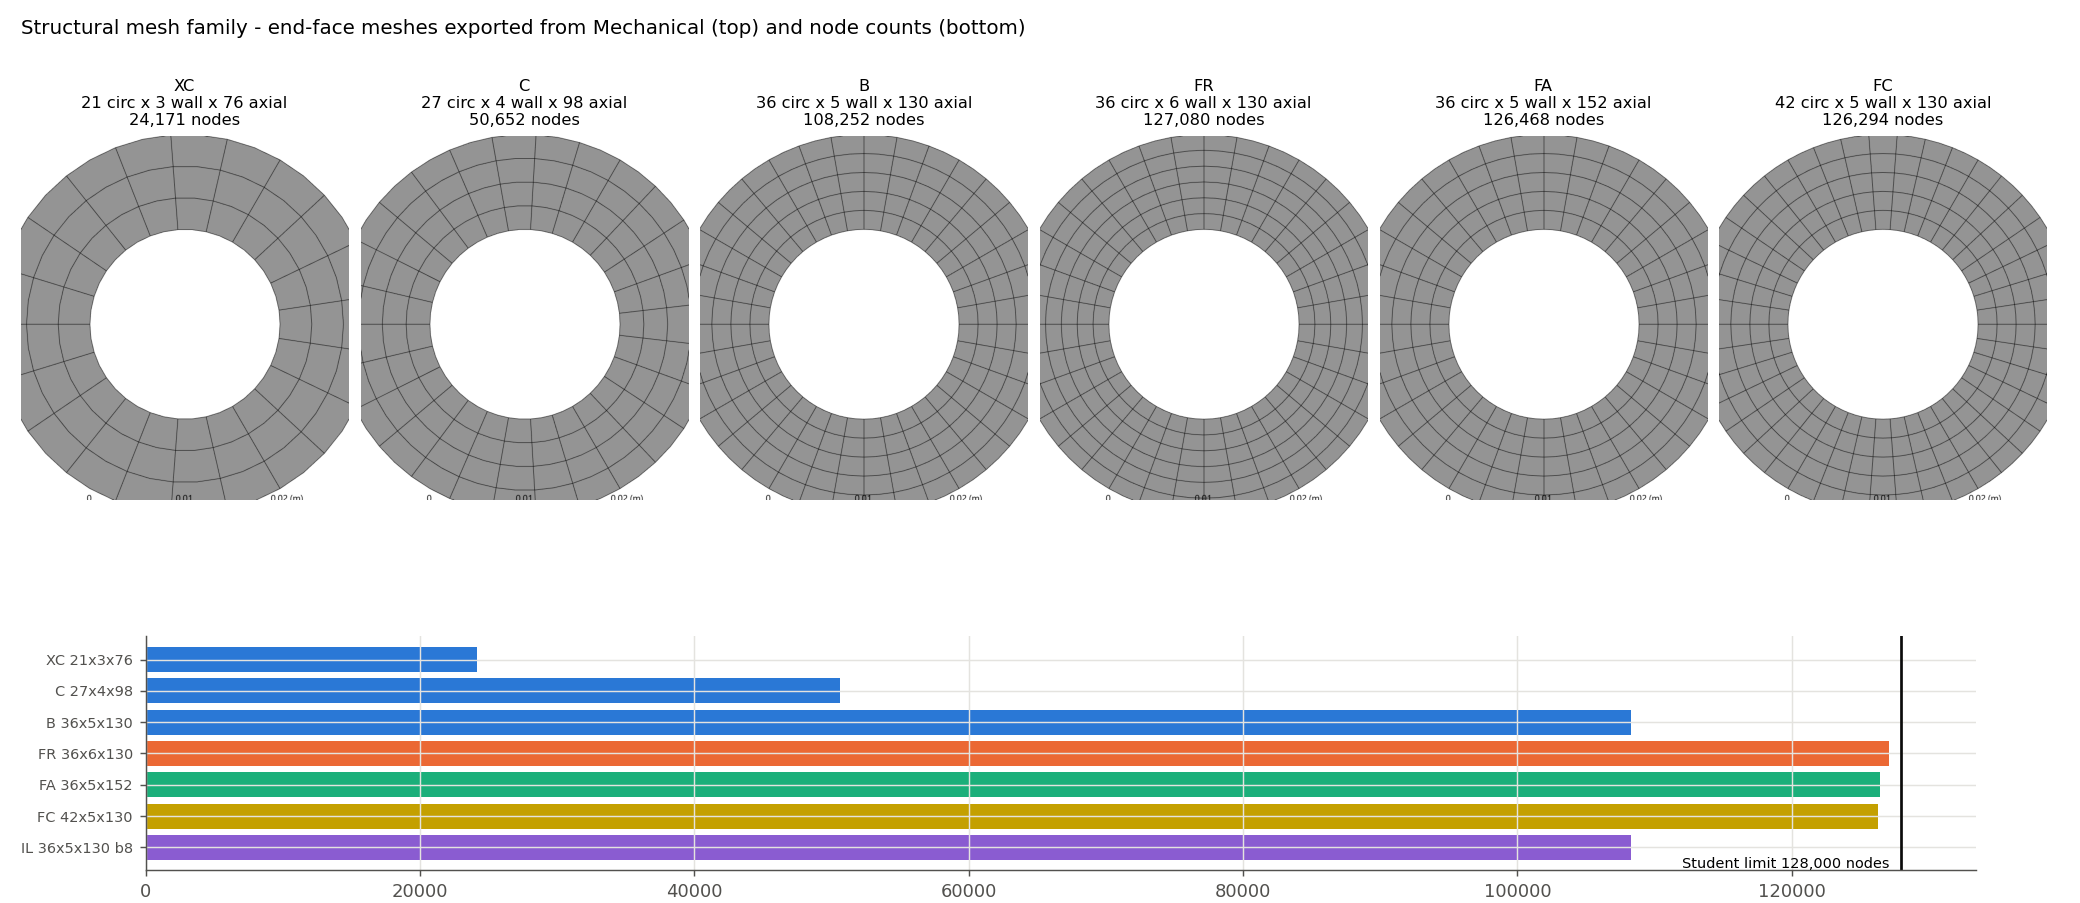
\includegraphics[width=0.86\linewidth]{F8B_01_structural_mesh_comparison.png}
\caption[Structural mesh family]{Structural mesh family: end-face meshes exported from Mechanical (top) and node counts against the 128,000-node Student limit (bottom).}
\label{fig:smfam}
\src{\provdata}
\end{figure}

\section{LC1 Sensitivity}
The LC1 deformation and free growth change by at most $3\times10^{-5}$ between meshes. The mid-span bore hoop stress is the only quantity with a
visible trend: on mesh B it is 18.309~MPa against a one-dimensional generalised-plane-strain exact value of 18.698~MPa
for the same imposed temperatures, $-$2.1\,\% ($-$1.5\,\% on FR). The interpolated temperature reproduces the exact solution within 0.1\,\%, so
the bias comes from surface-stress recovery on 2~mm quadratic elements; it is small in absolute terms (0.39~MPa) and its sign is known
(under-prediction). The LC1 inlet peak changes by +1.1\,\% (FR, FA), +0.9\,\% (IL) and $-$0.3\,\% (FC), far inside the $\pm$9.8~MPa
temperature-transfer bound.


\section{LC2 Sensitivity}
The governing LC2 results are converged. The peak von Mises stress is 605.161~MPa on B and changes by +0.0098\,\% (FR), $-$0.0035\,\% (FA),
+0.0015\,\% (FC) and $-$0.0045\,\% (IL); the coarsening family is monotonic and extrapolates to 605.187~MPa with a GCI of $5\times10^{-5}$. The
mean axial stress stays at $-$582.440~MPa within $7\times10^{-6}$ (Figure~\ref{fig:smlc2}).

\begin{figure}[htbp]
\centering
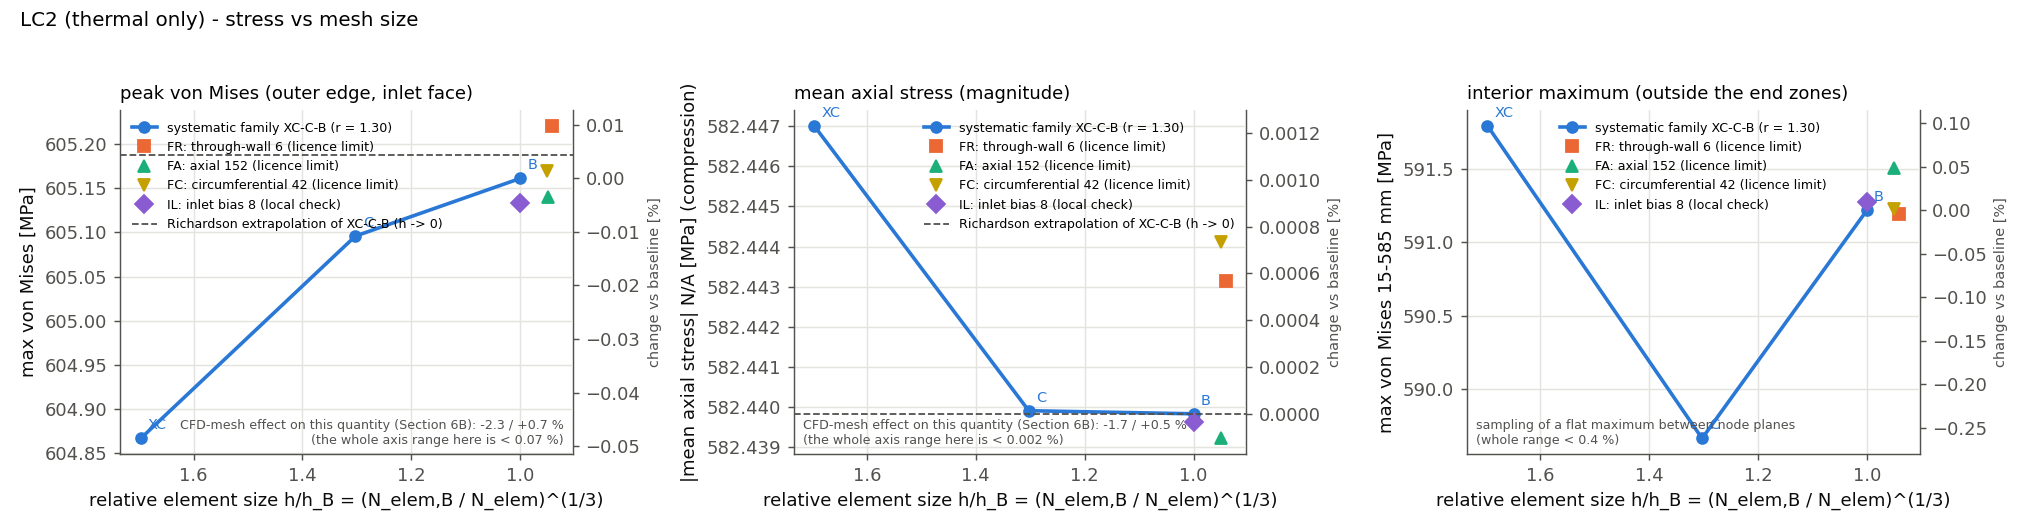
\includegraphics[width=0.92\linewidth]{F8B_02_LC2_stress_vs_mesh.png}
\caption[LC2 stresses against relative element size]{LC2 stresses against relative element size: peak von Mises at the inlet-face outer edge, mean axial stress and interior maximum.}
\label{fig:smlc2}
\src{\provdata}
\end{figure}

\section{Peak-Stress Behavior}
The LC2 peak sits at a physical location, the outer edge of the inlet face, and is identical on every mesh. It is not a singularity: the
difference between unaveraged and averaged nodal stresses there is $4\times10^{-5}$, and the peak is stable under every refinement to within
0.01\,\%. The symmetry-type face support $U_z = 0$ does not create an artificial stress concentration because it
restrains only the axial displacement of a plane face.


\section{Result Stability}
Across all seven meshes the largest change of the LC2 peak against mesh B is $4.9\times10^{-4}$ (on the coarsest mesh XC) and the largest
change of $\lambda_1$ is $5.4\times10^{-5}$; between the fine meshes and B, $\lambda_1$ changes by at most $6\times10^{-6}$ (Chapter~\ref{ch:buckling}).
The structural discretisation error is therefore one to two orders of magnitude smaller than the effect of the CFD mesh on the same quantities
(Chapter~\ref{ch:mi}) and several orders smaller than the effect of the supports (Chapter~\ref{ch:supports}).

\section{Final Structural Mesh}
Mesh B was retained for all further structural work (decision D-056). It is not the finest mesh, but the governing LC2 and buckling results are
converged on it; the fine meshes improve only the LC1 surface stresses, which drive no conclusion, while using 99\,\% of the licence. The
thickness cases use meshes with the same 2.0~mm radial element size (four and six elements through the 8 and 12~mm walls); check meshes with five
through-wall elements changed their LC2 mean stress and $\lambda_1$ by at most $4.2\times10^{-6}$ and their LC2 peak by at most $1.4\times10^{-4}$.

% ===================================================================== Chapter 13
\chapter{Buckling Analysis}\label{ch:buckling}

\section{Why Buckling Was Investigated}
The LC2 static state stores a compressive force of 548.94~kN in a column with a slenderness ratio $L/r$ of 53.67. A static stress check
alone cannot tell whether that state is stable: a yield utilisation of 0.578 says nothing about the load at which the straight equilibrium
bifurcates into a laterally deflected one. Because the LC2 restraint is exactly the condition that creates the compressive force, its
stability had to be examined before the static result could be interpreted.

\section{Applied Thermal Compression}
The column load is the LC2 end reaction, $N$ = 548,936.6~N, equivalent to a mean axial stress of 582.44~MPa over the section area of
942.48~mm$^2$. The 605.16~MPa von Mises peak is a local stress, not the column load. The load is thermal and displacement-controlled: it is
the force needed to hold the thermally expanded duct at its original length. In the linear buckling analysis the load factor $\lambda$
multiplies this entire thermal pre-stress; $\lambda$ = 1.108 therefore corresponds to about 10.8\,\% more restrained thermal strain, or
roughly 24~K more mean temperature rise.

\section{Euler Estimate}
Hand estimates were made before the FE analysis (Table~\ref{tab:section}), using Equation~\eqref{eq:euler} with a Rayleigh average of the
axially varying modulus $E(z)$ and, separately, with the shear correction. For the guided end condition of the LC2 supports ($K$ = 1) they give
load factors of 1.119 (Euler) and 1.104 (Euler + shear). All end conditions give intermediate columns ($KL/r$ below $C_c$ = 60.2), and the
elastic Euler stress of about 650~MPa exceeds the conventional proportional limit. The conventional Johnson estimate for the guided column
is 1.058, and the squash load corresponds to a factor of 1.755. Local or shell buckling is not credible: with $R/t$ = 1.5 the tube is far
outside thin-shell theory and compact by the round-HSS criterion $D/t < 0.11E/F_y$ ($4 < 20.2$) \cite{aisc360}.

%% generated by gen_tables.py - RE-ANALYSIS 2026
\begin{table}[htbp]
\centering
\footnotesize
\caption{Column properties and hand estimates of the buckling load factor (Section 8A)}
\label{tab:section}
\begin{tabular}{lrrr}
\toprule
End condition & $KL/r$ & Euler, $E(z)$ & Euler + shear \\
\midrule
Guided (rotation fixed, sway free) = S1 & 53.7 & 1.119 & 1.104 \\
Pinned--pinned & 53.7 & 1.114 & 1.099 \\
Fixed--pinned & 37.5 & 2.29 & 2.22 \\
Fixed--fixed (no sway) & 26.8 & 4.47 & 4.23 \\
\midrule
\multicolumn{4}{l}{$A$ = 942.48 mm$^2$; $I$ = 117,810 mm$^4$; $r$ = 11.18 mm; $L/r$ = 53.67; $C_c$ = 60.2; Johnson (guided) 1.058; squash 1.755} \\
\bottomrule
\end{tabular}
\par\smallskip\parbox{\linewidth}{\footnotesize\raggedright Source: \texttt{08\_Structural\_Analysis/Buckling/BUCKLING\_RESULTS.md} and \texttt{PROJECT\_STATE.md} \S15.1. Load factor = $P_{cr}/N$ with $N$ = 548,936.6 N. The shear correction uses the Engesser form with Cowper's coefficient $k$ = 0.620 \cite{cowper1966}.}
\end{table}


\section{ANSYS Linear Buckling}
The Eigenvalue Buckling system was linked to the LC2 static solution in a save-as copy of the project, as a perturbation restart that keeps
all LC2 boundary conditions. The re-solved LC2 pre-stress in the copy reproduced the Section 7B values exactly (peak von Mises and end
reaction). The full 108,252-node model solved within the Student licence. Before the project model was solved, the workflow was benchmarked
on a constant-property toy tube whose Euler loads are known in closed form for both end conditions.

\section{Mode Shapes}
The first mode (Figure~\ref{fig:bkmode}) is a global column mode: the end planes stay perpendicular to the axis but translate sideways in
opposite directions; the lateral deflection is zero at mid-span and the bending curvature is largest at the rotation-held end sections. The
cross-section moves as a rigid section (99.9999\,\%); there is no ovalisation, shell or local mode. The shape correlates with
$\cos(\pi z/L)$ to 0.999997. Modes 1 and 2 are an orthogonal pair with the same eigenvalue, as expected for an
axisymmetric column.

\begin{figure}[htbp]
\centering
\begin{subfigure}[t]{0.49\linewidth}\centering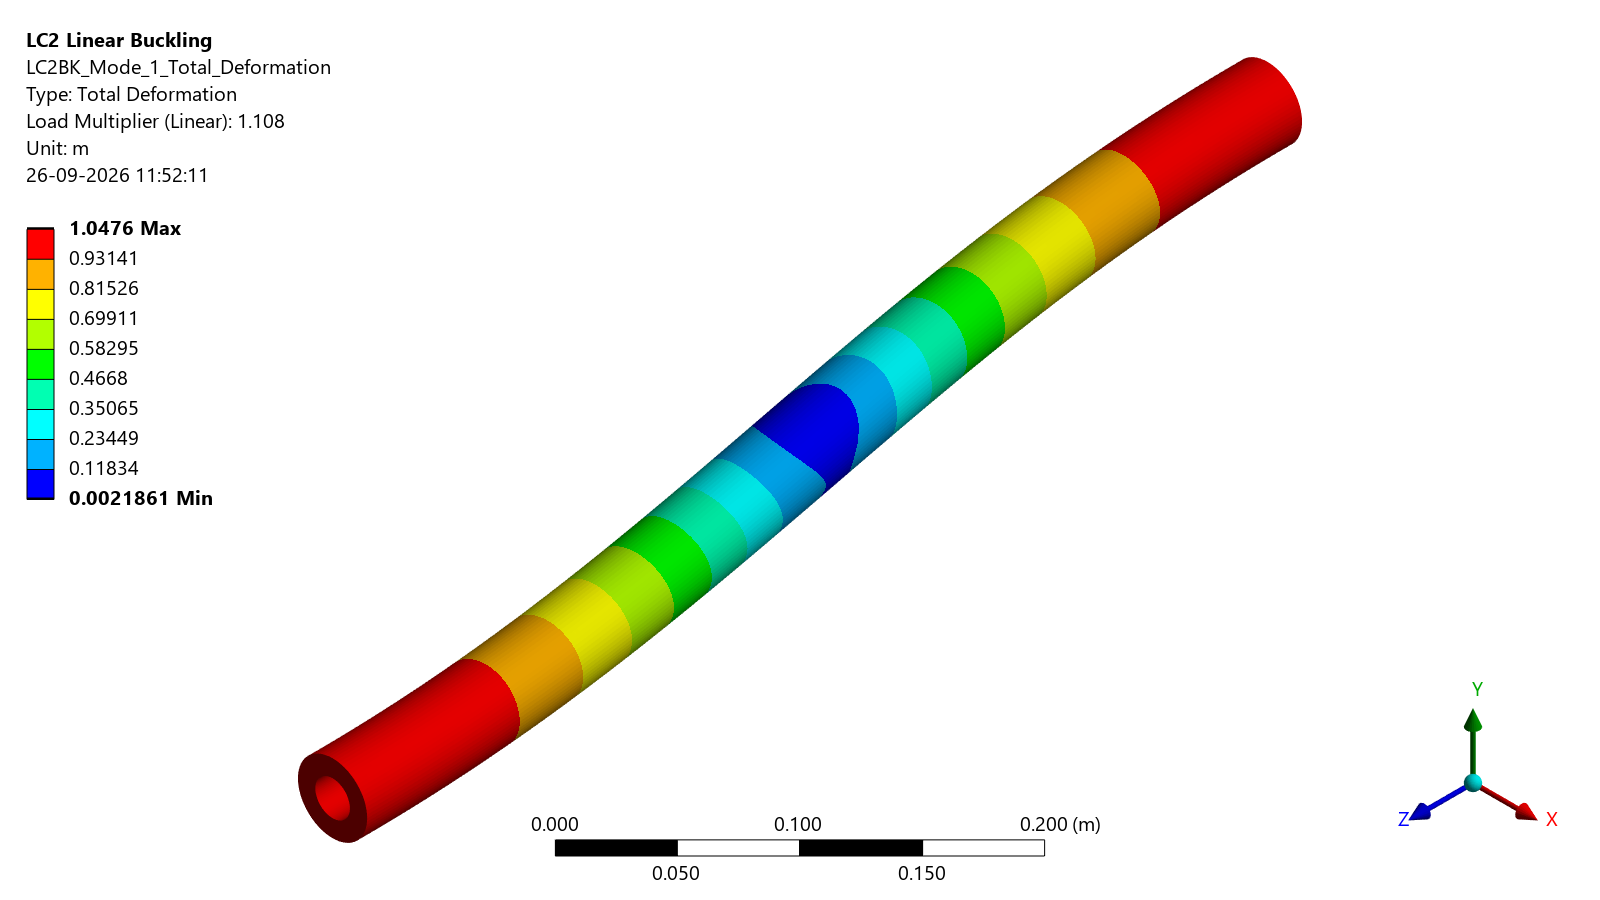
\includegraphics[width=\linewidth,height=52mm,keepaspectratio]{LC2_Linear_Buckling_Mode_1_Total_Deformation_iso.png}\caption{Isometric view}\end{subfigure}\hfill
\begin{subfigure}[t]{0.49\linewidth}\centering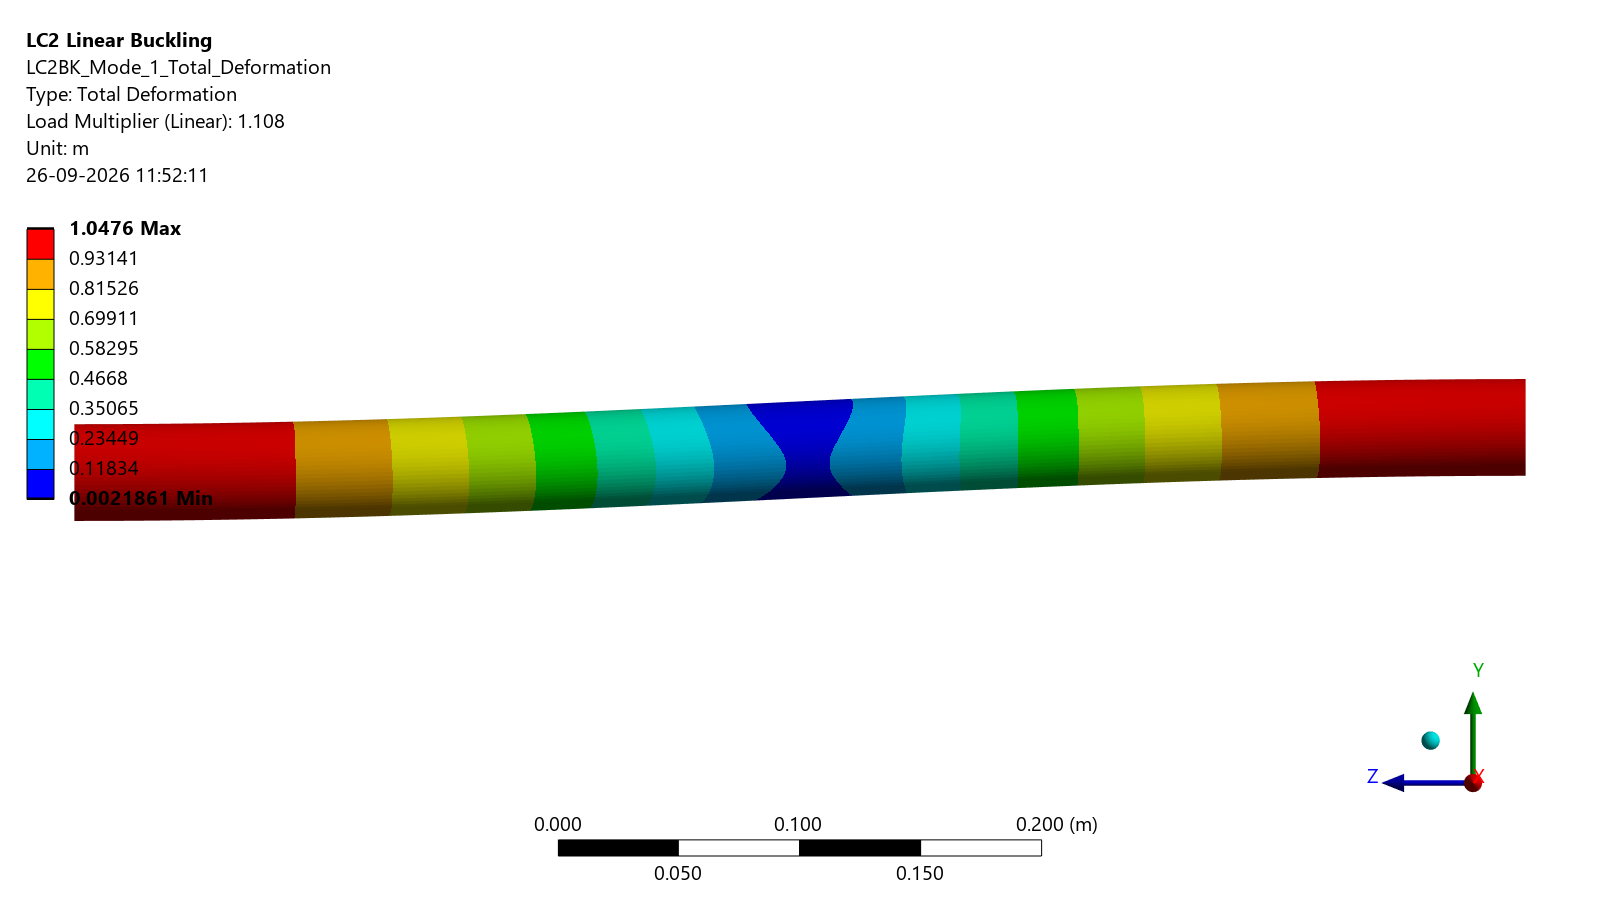
\includegraphics[width=\linewidth,height=52mm,keepaspectratio]{LC2_Linear_Buckling_Mode_1_Total_Deformation_side_YZ.png}\caption{Side view}\end{subfigure}
\caption[First buckling mode of the restrained duct under S1]{First buckling mode of the restrained duct under S1 (load multiplier 1.108; normalised eigenvector, amplitude arbitrary).}
\label{fig:bkmode}
\src{\provmech}
\end{figure}


\section{Buckling Factor}
The first eigenvalue is $\lambda_1$ = 1.108 (Table~\ref{tab:buckling}), giving a critical load $P_{cr} = \lambda_1 N$ = 608.25~kN. The next
eigenvalue pair is 4.298. The FE value lies between the Euler estimate with $E(z)$ ($-$1.0\,\%) and the shear-corrected estimate (+0.4\,\%),
which is the expected position for a stocky tube (Figure~\ref{fig:bkpcr}).

%% generated by gen_tables.py - RE-ANALYSIS 2026
\begin{table}[htbp]
\centering
\footnotesize
\caption{Linear eigenvalue buckling results of the baseline under S1 (Section 8A)}
\label{tab:buckling}
\begin{tabular}{>{\raggedright\arraybackslash}p{0.45\linewidth}r}
\toprule
Quantity & Value \\
\midrule
Applied axial compression $N$ (LC2 end reaction) [N] & 548,936.6 \\
$\lambda_1 = \lambda_2$ (orthogonal pair) & 1.10805 \\
Next eigenvalue pair & 4.298 \\
Critical load $P_{cr} = \lambda_1 N$ [kN] & 608.25 \\
Dominant mode & global guided-column sway, $\cos(\pi z/L)$ \\
First-yield load factor (LC2) & 1.730 \\
Conventional inelastic (Johnson) estimate & 1.058 \\
\bottomrule
\end{tabular}
\par\smallskip\parbox{\linewidth}{\footnotesize\raggedright Source: \texttt{MASTER\_PROJECT\_DATA.csv} rows M091, M096, M098--M100, M107; \texttt{BUCKLING\_RESULTS.md}. $\lambda_1$ is an idealised linear stability indicator, not a collapse load and not a factor of safety.}
\end{table}


\begin{figure}[htbp]
\centering
\begin{subfigure}[t]{0.49\linewidth}\centering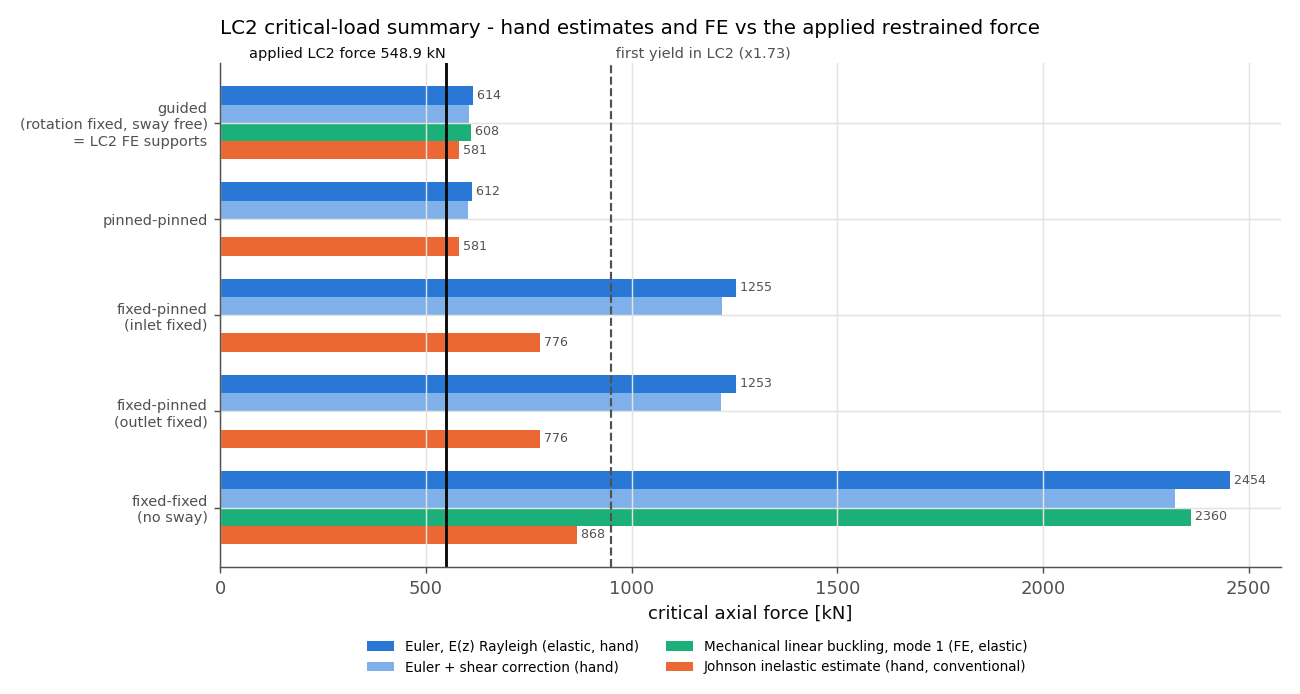
\includegraphics[width=\linewidth,height=52mm,keepaspectratio]{F8A_03_critical_load_summary.png}\caption{Critical axial force [kN]}\end{subfigure}\hfill
\begin{subfigure}[t]{0.49\linewidth}\centering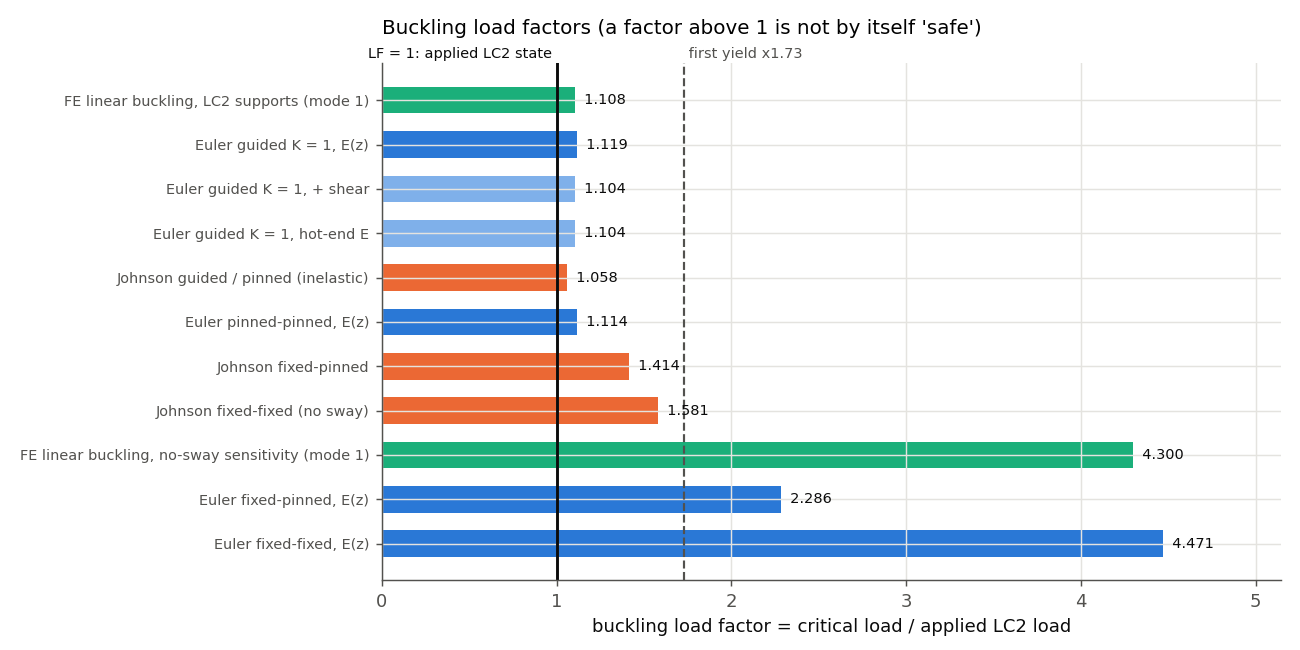
\includegraphics[width=\linewidth,height=52mm,keepaspectratio]{F8A_04_load_factor_comparison.png}\caption{Buckling load factors}\end{subfigure}
\caption[Hand estimates and FE results against the applied restrained force]{Hand estimates and FE results against the applied restrained force: elastic Euler, shear-corrected, conventional Johnson (inelastic) and FE linear buckling.}
\label{fig:bkpcr}
\src{\provdata}
\end{figure}

\section{Buckling Mesh Sensitivity}
The same buckling analysis was repeated on the six meshes of Chapter~\ref{ch:smesh} that carry a buckling solution (Table~\ref{tab:appF}). $\lambda_1$ ranges from 1.1079876 (XC) to 1.1080483 (FA); the coarsening family is monotonic with a GCI of
$5.6\times10^{-6}$, and the fine meshes lie within $6\times10^{-6}$ of mesh B. The mode is the same guided-sway shape on every mesh. The buckling
result is not sensitive to the structural mesh.


\section{Yield vs Buckling}
Two different load factors describe the idealised LC2 state and are reported side by side:
\begin{itemize}
\item the first-yield factor, 1.730: the thermal load multiplier at which the most highly stressed point reaches the local yield strength;
\item the linear buckling factor, $\lambda_1$ = 1.108: the multiplier at which the perfect, elastic column bifurcates.
\end{itemize}
Because $\lambda_1$ is below the first-yield factor, the idealised S1 model is stability-limited: elastic bifurcation is reached before first
yield. With $\lambda_1$ this close to 1, the idealised model is close to instability at the applied thermal load. The yield utilisation of
0.578 is therefore not a structural margin. Expressed on the Section 2 temperature basis (254.7~K mean rise instead of 225.5~K), the same
analysis would give $\lambda_1 \approx$ 0.98. No single factor of safety is formed in this project.

\section{Limitations of Linear Eigenvalue Buckling}
$\lambda_1$ is a linear stability indicator for an idealised elastic model. It is \textbf{not} a guaranteed real-world collapse load. The
analysis assumes:
\begin{itemize}
\item a perfectly straight tube without out-of-straightness, load eccentricity or residual stress;
\item linear elastic material, although the columns are intermediate and the elastic buckling stress exceeds the proportional limit;
\item small deflections, with no post-buckling path;
\item idealised supports whose relation to a real flange is undefined.
\end{itemize}
A real, imperfect duct would deflect laterally at loads below $\lambda_1$, and inelastic behaviour lowers its capacity further; the
conventional Johnson estimate of 1.058 indicates the direction of that reduction, not its material-specific size. Rotational flexibility of
real end fixtures would lower $\lambda_1$ below the S1 value, so S1 is not a lower bound. An imperfection-sensitive, geometrically and
materially nonlinear analysis would be required to determine a collapse load (Chapter~\ref{ch:future}). An elastic, geometrically
nonlinear imperfection-sensitivity extension is reported in Section~\ref{sec:lsdyna}; it does not determine a collapse load.

% ===================================================================== Chapter 14
\chapter{Support Sensitivity}\label{ch:supports}

\section{Importance of End Restraint}
The end supports enter the problem twice. Axially, they decide whether the thermal growth is free (LC1) or prevented (LC2), and hence whether
a compressive force exists at all. Laterally and rotationally, they set the effective length of the resulting column and therefore its
buckling load. The real flange of the duct is not defined in this project, so three idealised scenarios with the same axial
restraint but different lateral and rotational restraint were analysed at the baseline design (Table~\ref{tab:support}). They are listed
in the order in which they were defined; they are not a ranking.

%% generated by gen_tables.py - RE-ANALYSIS 2026
\begin{table}[htbp]
\centering
\footnotesize
\caption{Support sensitivity at the baseline design (listed in order of definition, not ranked)}
\label{tab:support}
\begin{tabular}{lrrrl>{\raggedright\arraybackslash}p{0.20\linewidth}}
\toprule
Scenario & Max VM [MPa] & $\lambda_1$ & $P_{cr}$ [kN] & Mode & Mechanism first reached \\
\midrule
S1 guided ($K$ = 1) & 605.161 & 1.10805 & 608.25 & guided sway & elastic bifurcation (1.108 $<$ 1.730) \\
S2 clamped--clamped ($K$ = 0.5) & 605.160 & 4.29995 & 2,360.40 & clamped column & first yield (1.730 $<$ 4.300) \\
S3 clamped--pinned ($K$ = 0.699) & 605.160 & 2.23224 & 1,225.36 & fixed--pinned & first yield (1.730 $<$ 2.232) \\
\bottomrule
\end{tabular}
\par\smallskip\parbox{\linewidth}{\footnotesize\raggedright Source: \texttt{MASTER\_PROJECT\_DATA.csv} rows M090, M098--M110. End reaction 548,936.6~N and mean axial stress $-$582.44~MPa in all three scenarios. The mechanism column compares $\lambda_1$ with the first-yield factor of the idealised model only.}
\end{table}


\section{S1}
S1 is the LC2 support of the baseline: both end faces are held axially over their full area, which keeps them plane and prevents end rotation,
while the ends remain free to translate sideways. Structurally this is a guided (sway) column with $K = 1$. Its first mode is the sway mode of
Figure~\ref{fig:bkmode} with $\lambda_1$ = 1.108 and $P_{cr}$ = 608.25~kN.

\section{S2}
S2 adds lateral restraint at both ends ($U_\theta = 0$ on every end-face node): both ends are clamped against translation and rotation
($K = 0.5$). The first mode becomes the clamped-column shape with its maximum at mid-span (Figure~\ref{fig:s2s3}a), and $\lambda_1$ rises to
4.300 ($P_{cr}$ = 2,360.40~kN). The corresponding elastic buckling stress would be about 2500~MPa, far above yield, so a laterally held duct
would reach first yield or inelastic buckling long before this elastic bifurcation (Johnson estimate 1.58, squash 1.755).

\section{S3}
S3 clamps the inlet face and pins the outlet: the outlet face is tied to a deformable remote point on the axis that is held in position but
free to rotate ($K = 0.699$). This was the first use of a remote-point support in the project, so the exact formulation written by Mechanical
(pilot node with target element, contact elements on the outlet faces, bonded multipoint constraint) was first copied into the constant-property
toy tube (benchmark B03). The benchmark passed in two runs: the reactions matched $E\alpha\Delta T A$, no rigid-body motion occurred, and the toy
$\lambda_1$ of 2.2377 fell between the plain (2.2908) and shear-corrected (2.2256) fixed--pinned Euler values. The real S3 case then gave
$\lambda_1$ = 2.232 ($P_{cr}$ = 1,225.36~kN) with the fixed--pinned mode shape, maximum lateral deflection at 0.605 $L$ from the clamped end
(Figure~\ref{fig:s2s3}b).

\begin{figure}[htbp]
\centering
\begin{subfigure}[t]{0.49\linewidth}\centering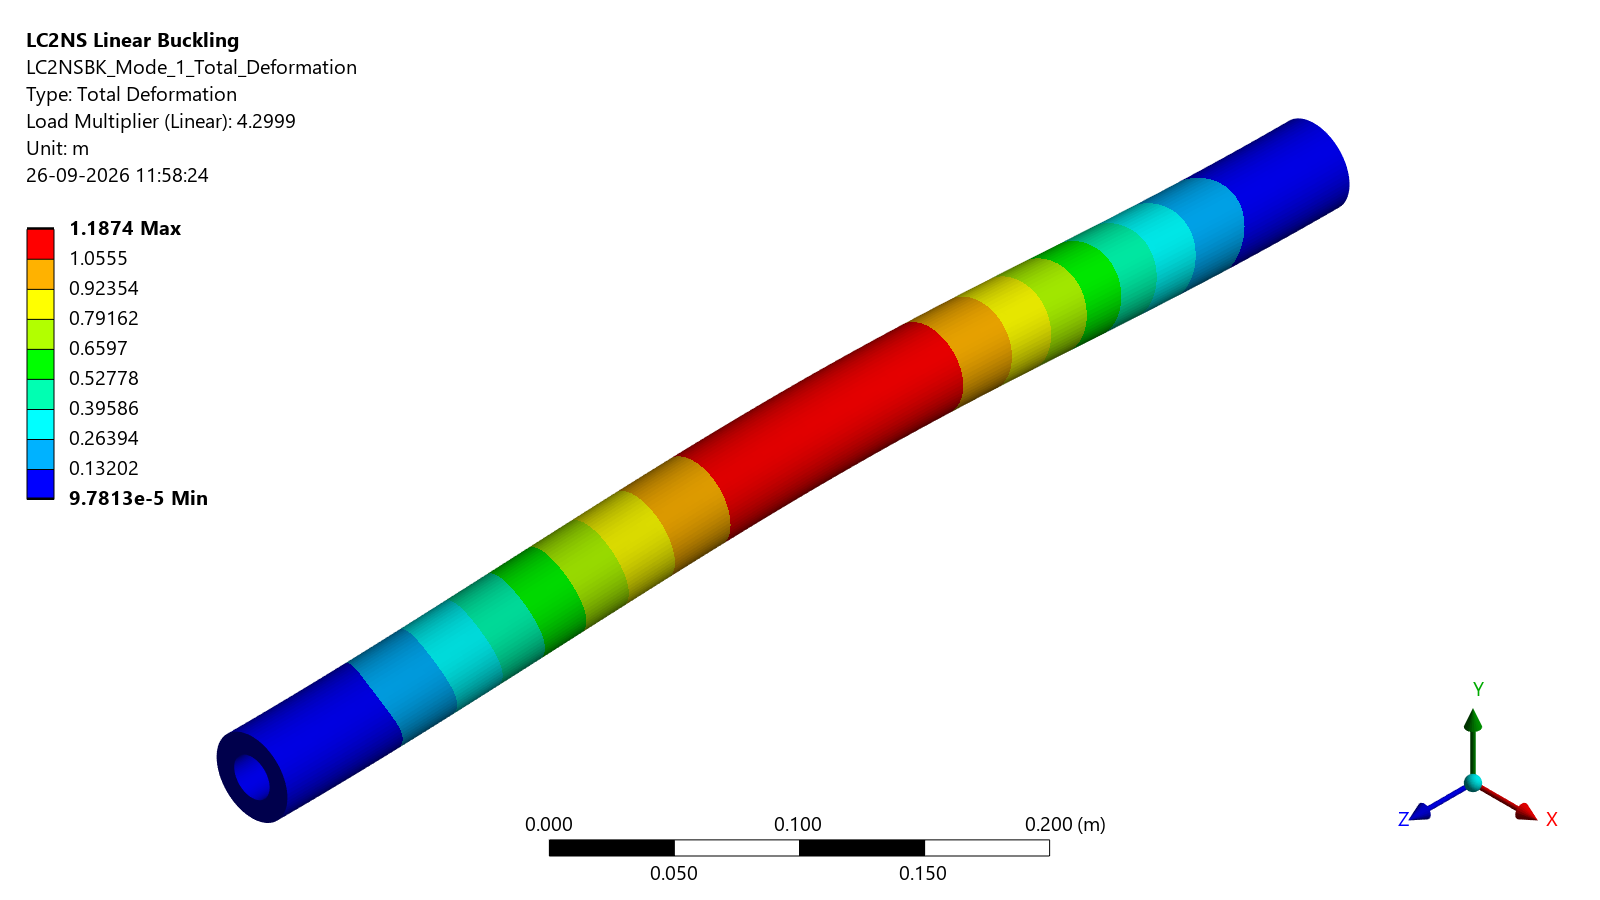
\includegraphics[width=\linewidth,height=52mm,keepaspectratio]{LC2NS_Linear_Buckling_Mode_1_Total_Deformation_iso.png}\caption{S2, both ends clamped (load multiplier 4.2999)}\end{subfigure}\hfill
\begin{subfigure}[t]{0.49\linewidth}\centering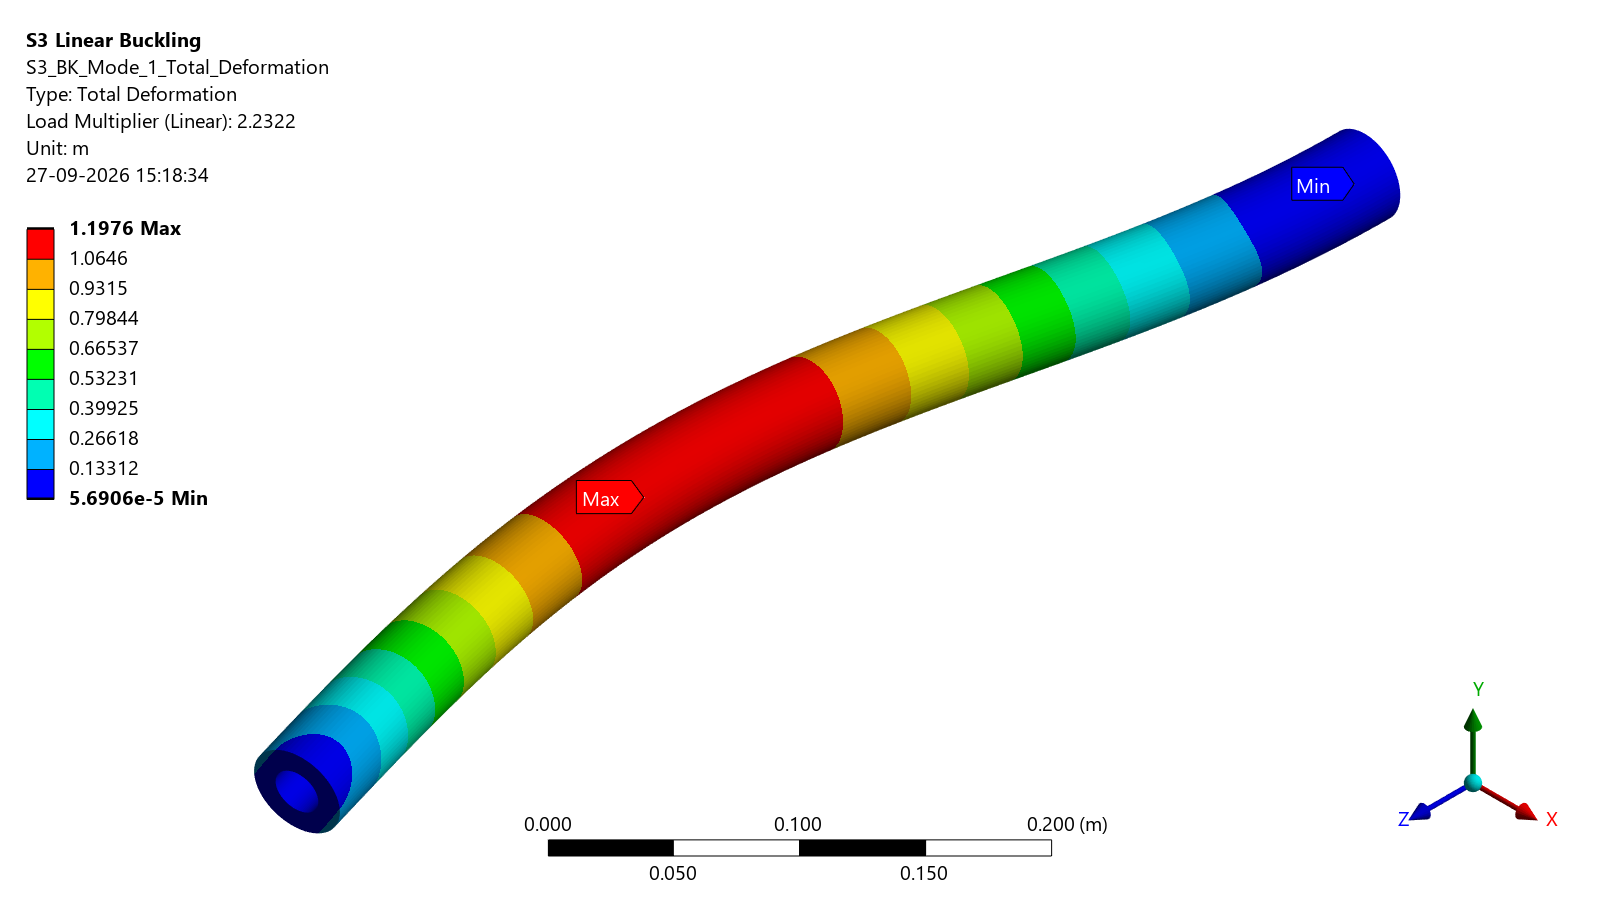
\includegraphics[width=\linewidth,height=52mm,keepaspectratio]{S3_BK_Mode_1_iso.png}\caption{S3, clamped--pinned (load multiplier 2.2322)}\end{subfigure}
\caption{First buckling modes of the support-sensitivity scenarios (normalised eigenvectors).}
\label{fig:s2s3}
\src{\provmech}
\end{figure}

\section{Buckling-Factor Sensitivity}
The static state is identical in all three scenarios to better than 0.01\,\%: peak von Mises 605.16~MPa, mean axial stress $-$582.44~MPa and
end force 548,936.6~N (Figure~\ref{fig:supp}b). The stability, by contrast, changes by a factor of 3.9: the FE ratios S1 : S3 : S2 are
1 : 2.015 : 3.881, close to the Euler ratios 1 : 2.047 : 4 for $K$ = 1, 0.699 and 0.5 (Figure~\ref{fig:supp}a). Greater lateral and rotational
restraint of the ends shortens the effective length and raises the idealised buckling factor. The governing mechanism changes with it: under
S1 the elastic bifurcation comes before first yield (1.108 $<$ 1.730); under S2 and S3 first yield comes first (1.730 $<$ 2.232 and 4.300).

\begin{figure}[htbp]
\centering
\begin{subfigure}[t]{0.49\linewidth}\centering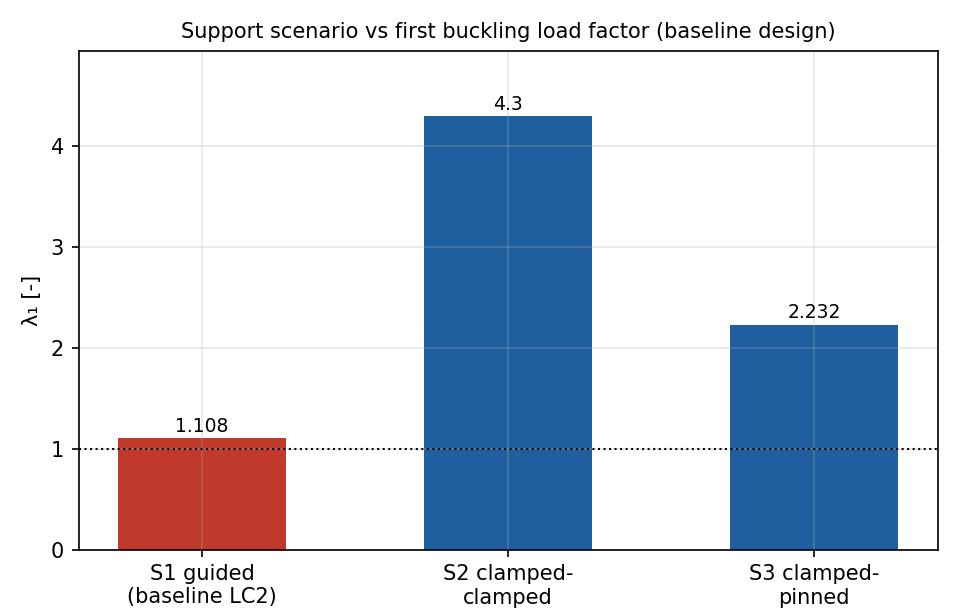
\includegraphics[width=\linewidth,height=52mm,keepaspectratio]{F14_support_vs_lambda1.png}\caption{First buckling load factor $\lambda_1$}\end{subfigure}\hfill
\begin{subfigure}[t]{0.49\linewidth}\centering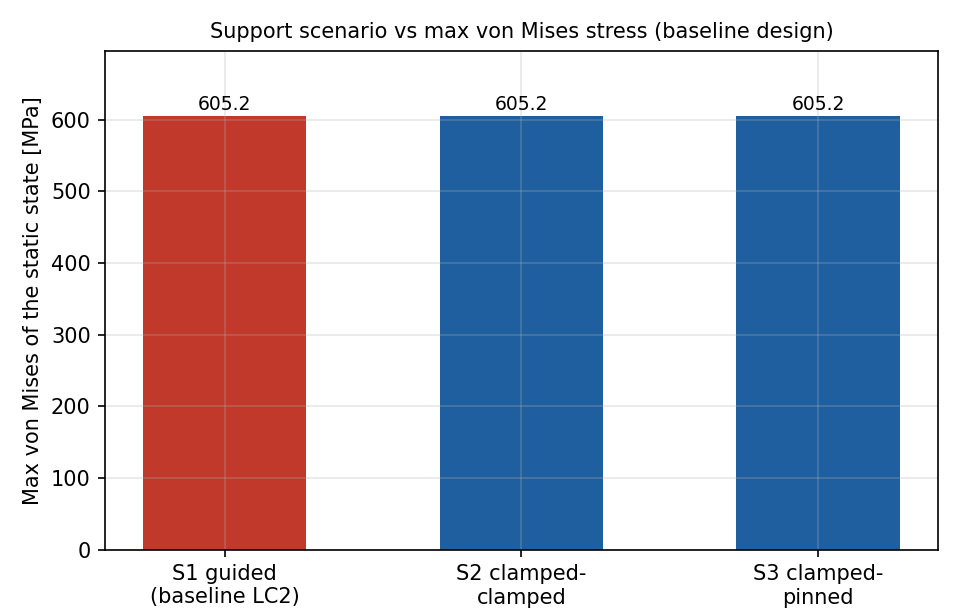
\includegraphics[width=\linewidth,height=52mm,keepaspectratio]{F15_support_vs_LC2_stress.png}\caption{Maximum von Mises stress of the static state [MPa]}\end{subfigure}
\caption[Support sensitivity at the baseline design]{Support sensitivity at the baseline design: stability depends strongly on the end restraint, the static stress does not.}
\label{fig:supp}
\src{\provdata}
\end{figure}

\section{Implications of Support Uncertainty}
The end-support definition is the largest single uncertainty in the structural conclusion. A beam-column estimate calibrated to the FE
results (rotation-fixed ends) shows the relative lateral stiffness between the ends that would be needed: about 0.45~kN/mm for $\lambda_1$ =
1.5, about 0.71~kN/mm to reach the first-yield factor of 1.73, and about 3.9~kN/mm for full no-sway behaviour. Conversely, rotational
flexibility of real flanges would lower $\lambda_1$ below the S1 value (a conceptual $K$ = 2 gives about 0.28). None of S1, S2 or S3 is
therefore a bound on a real installation, and none is recommended here: the scenarios show the model's response to a boundary condition that
must be defined from the real mounting design before any statement about the stability of a component can be made (open task T-034).

% ===================================================================== Chapter 14 (continued)
% Additional nonlinear buckling analysis using ANSYS LS-DYNA (follow-on extension; values from
% 15_LS_DYNA_Extension/12C_Nonlinear_Buckling: FINAL_12C_RESULTS.md, IMPERFECTION_SENSITIVITY.csv, MECHANICAL_vs_LSDYNA.csv)
\section{Additional Nonlinear Buckling Analysis Using ANSYS LS-DYNA}\label{sec:lsdyna}
This section reports an additional nonlinear buckling analysis using ANSYS LS-DYNA, carried out as a follow-on extension of the
thermo-structural analysis of Chapters~\ref{ch:buckling} and~\ref{ch:supports}. It is not part of the internship work programme described in
Chapter~\ref{ch:intro} and does not change any result of the preceding chapters; the Mechanical linear buckling result ($\lambda_1$ = 1.108,
$P_{cr}$ = 608.25~kN under S1) remains the reference.

\subsection{Purpose and Model}
The linear eigenvalue analysis gives the bifurcation load of a perfectly straight, elastic column (Chapter~\ref{ch:buckling}). It cannot show how a duct
with an initial out-of-straightness deflects as the thermal load rises. The extension therefore follows the geometrically nonlinear
(large-deflection) load path of the S1 / LC2 configuration with small imperfections in the shape of the first buckling mode.

The LS-DYNA model is the LC2 model of Chapter~\ref{ch:struct} carried over unchanged:
\begin{itemize}
\item the same mesh (108,252 nodes, 23,400 twenty-node solid elements);
\item the same CFD-derived temperature field mapped from the medium Fluent solution, with the reference temperature of 300~K;
\item the same LC2 support condition (S1);
\item temperature-dependent elastic Inconel~718 properties.
\end{itemize}
Before any nonlinear run, the LS-DYNA model was verified against Mechanical. The static LC2 state gives a peak von Mises stress of
605.160~MPa against 605.161~MPa at the same location. The LS-DYNA linear buckling factor is 1.1095, +0.13\,\% from the Mechanical value, or
$-$0.64\,\% after the documented large-deformation effect is removed. The mode shape agrees with the Mechanical mode~1 to 0.9999998.

In the nonlinear analysis the temperature rise above 300~K is scaled by a load parameter $\lambda$ up to 1.3. The load steps are fine
($\Delta\lambda$ = 0.005) between $\lambda$ = 1.0 and 1.2, around the expected instability. The imperfection is the normalised first buckling
mode, applied with peak lateral amplitudes of 0.1~mm (case C1), 0.6~mm (C3) and 1.2~mm (C5). These amplitudes are numerical sensitivity
values, not manufacturing tolerances. A perfect-geometry run (C0) serves as a reference path. All four runs terminated normally.

\subsection{Results}
Table~\ref{tab:lsdyna} summarises the three-point imperfection sensitivity study, and Figure~\ref{fig:lsdpath} shows the load paths.

\begin{itemize}
\item \textbf{Load path.} All imperfect cases deflect laterally from the start of loading. The axial compression $N$ (the end reaction)
      flattens towards the critical load as the deflection grows.
\item \textbf{Effect of amplitude below the critical load.} The imperfection amplitude governs where the response leaves the perfect path,
      defined here as $N$ falling 1\,\% below the perfect-geometry value: at $\lambda$ = 1.070 (C1), 0.825 (C3) and 0.375 (C5). It also governs
      the response at the LC2 temperature field ($\lambda$ = 1):
      \begin{itemize}
      \item $N$ is 552.2, 531.2 and 503.5~kN;
      \item the peak von Mises stress is 690, 966 and 1104~MPa;
      \item the end faces translate sideways by 0.85, 3.71 and 5.32~mm.
      \end{itemize}
\item \textbf{Maximum load.} The smallest imperfection reaches a maximum of 601.0~kN at $\lambda$ = 1.185 and then decreases slowly while the
      sway continues to grow. C3 and C5 are still rising at the end of the analysis ($\lambda$ = 1.3), at 572.4 and 545.3~kN.
\item \textbf{Characteristic load.} Southwell plots of the pre-critical branches give 612.3 (C1), 611.1 (C3) and 607.7~kN (C5).
\end{itemize}

%% Section 13 - additional LS-DYNA analysis; values from 15_LS_DYNA_Extension/12C_Nonlinear_Buckling/IMPERFECTION_SENSITIVITY.csv
\begin{table}[htbp]
\centering
\footnotesize
\setlength{\tabcolsep}{3.4pt}
\caption{Additional LS-DYNA nonlinear analysis: three-point imperfection sensitivity under S1 / LC2 (elastic, geometrically nonlinear)}
\label{tab:lsdyna}
\begin{tabular}{l r r r r r >{\raggedright\arraybackslash}p{0.155\linewidth} r r}
\toprule
Case & $A$ [mm] & 1\,\% drop $\lambda$ & $N$ ($\lambda$ = 1) [kN] & VM ($\lambda$ = 1) [MPa] & Yield $\lambda$ & Maximum $N$ ($\lambda \le$ 1.3) & Southwell [kN] & vs $P_{cr}$ \\
\midrule
C1 & 0.1 & 1.070 & 552.2 & 690 & 1.109 & 601.0~kN at $\lambda$ = 1.185 (maximum) & 612.3 & +0.7\,\% \\
C3 & 0.6 & 0.825 & 531.2 & 966 & 1.031 & 572.4~kN at $\lambda$ = 1.3, still rising & 611.1 & +0.5\,\% \\
C5 & 1.2 & 0.375 & 503.5 & 1104 & 0.974 & 545.3~kN at $\lambda$ = 1.3, still rising & 607.7 & $-$0.1\,\% \\
\midrule
C0 (perfect) & 0 & -- & 553.2 & 605.2 & not reached & no instability flagged (720.7~kN at $\lambda$ = 1.3) & \multicolumn{2}{l}{not identifiable} \\
\bottomrule
\end{tabular}
\par\smallskip\parbox{\linewidth}{\footnotesize\raggedright Source: \texttt{15\_LS\_DYNA\_Extension/12C\_Nonlinear\_Buckling/IMPERFECTION\_SENSITIVITY.csv} and \texttt{FINAL\_12C\_RESULTS.md} (additional LS-DYNA analysis); Mechanical reference $\lambda_1$ = 1.108 and $P_{cr}$ = 608.25~kN from \texttt{MASTER\_PROJECT\_DATA.csv} rows M098--M099. $A$: imperfection amplitude. 1\,\% drop: $\lambda$ at which $N$ falls 1\,\% below the perfect path. $N$: axial compression (end reaction); VM: peak von Mises stress. Yield $\lambda$: first local yield, i.e.\ the peak von Mises stress equals the local yield estimate $S_y(T)$ of the elastic model. The perfect-geometry run C0 is a reference path; its $N$ at $\lambda$ = 1 is 0.79\,\% above the Mechanical 548.94~kN because of the large-deformation formulation. Load values are not factors of safety.}
\end{table}


\begin{figure}[htbp]
\centering
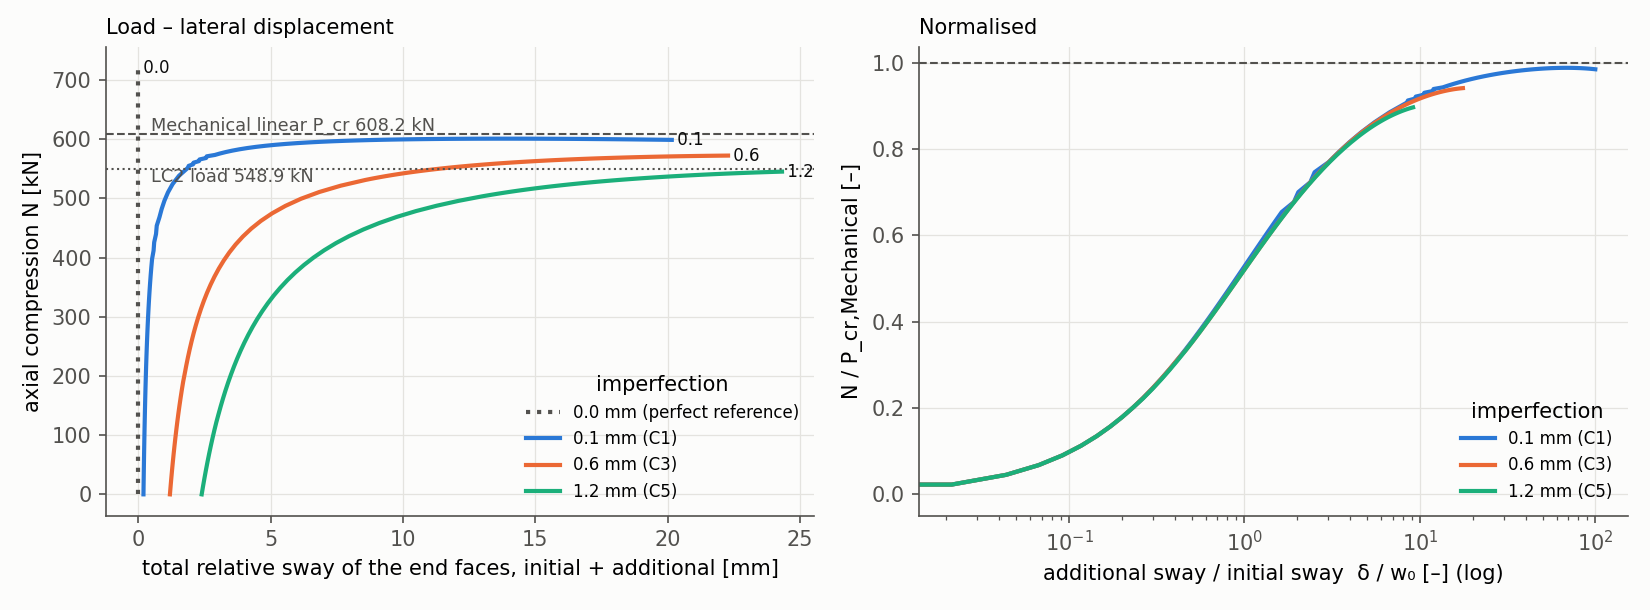
\includegraphics[width=\linewidth,keepaspectratio]{LSD_load_lateral_nt.png}
\caption[Additional LS-DYNA analysis: axial compression against lateral end sway]{Additional LS-DYNA analysis: axial compression against the
total relative sway of the end faces for the three imperfection amplitudes and the perfect-geometry reference (left), and the same paths
normalised by the Mechanical critical load and the initial sway (right).}
\label{fig:lsdpath}
\src{Plotted with matplotlib from the LS-DYNA solver output (binout and nodout) of the additional analysis; title strip cropped.}
\end{figure}

\subsection{Comparison with the Mechanical Linear Buckling Result}
The Southwell characteristic-load estimates of 607.7--612.3~kN lie within $-$0.1\,\% to +0.7\,\% of the Mechanical critical load of
608.25~kN ($\lambda_1$ = 1.108), as shown in Figure~\ref{fig:lsdcomp}.

\begin{itemize}
\item \textbf{Imperfection-sensitive response.} The amplitude strongly affects:
      \begin{itemize}
      \item the onset of lateral deformation;
      \item the displacement and stress at a given load;
      \item the maximum load reached within $\lambda \le$ 1.3: 98.8, 94.1 and 89.7\,\% of $P_{cr}$.
      \end{itemize}
\item \textbf{Insensitive characteristic load.} The characteristic global buckling load is relatively insensitive to the tested amplitudes
      and supports the magnitude of the linear eigenvalue prediction.
\item \textbf{Perfect-geometry run.} C0 stays straight beyond $P_{cr}$ (720.7~kN at $\lambda$ = 1.3) without flagging a bifurcation, because
      the solver ignores negative eigenvalues by default. A perfect-geometry bifurcation load is therefore not identifiable from the LS-DYNA
      analysis, and the Mechanical eigenvalue remains the linear perfect-geometry reference.
\item \textbf{Global mode.} In every case the response is a global sideways (guided-sway) bending of the whole duct, the same shape as
      Mechanical mode~1 (Figure~\ref{fig:lsdshape}):
      \begin{itemize}
      \item the mid-span lateral displacement stays below 0.2\,\% of the end-face translation;
      \item the ovalisation is at most 0.041~mm;
      \item there is no local or shell-type mode;
      \item the highest stress is at the outer edge of the inlet face, the critical location of Chapter~\ref{ch:struct}.
      \end{itemize}
\end{itemize}
None of these load values is a factor of safety or a real-world capacity, and the analysis is not an experimental validation.

\begin{figure}[htbp]
\centering
\begin{subfigure}[t]{\linewidth}\centering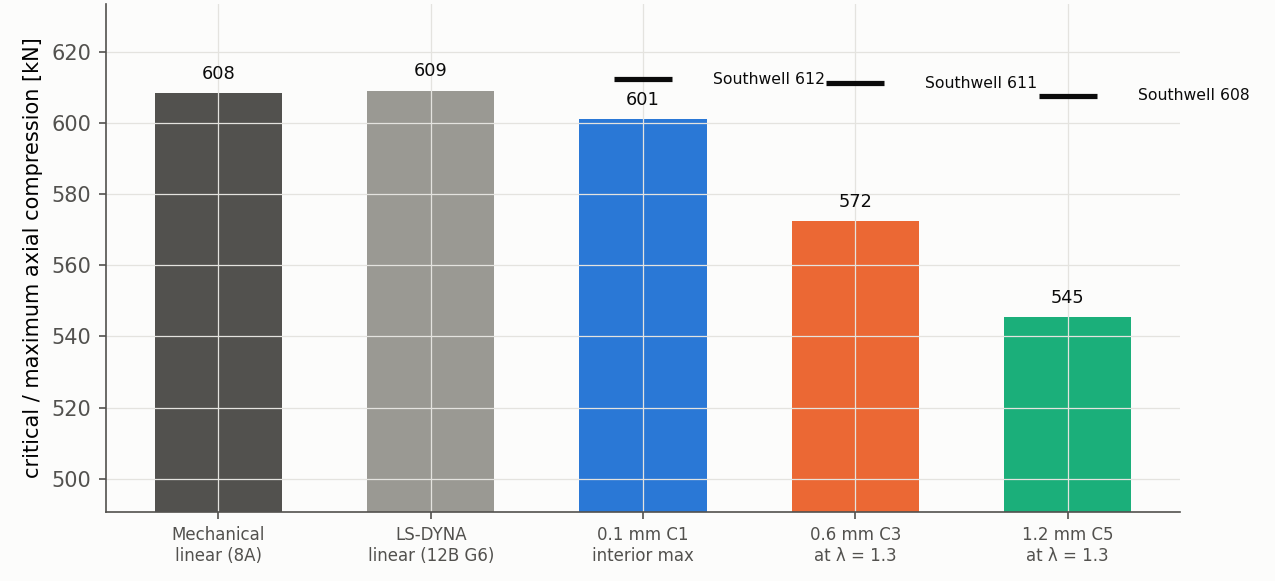
\includegraphics[width=0.78\linewidth,keepaspectratio]{LSD_mechanical_vs_nonlinear_nt.png}\caption{Mechanical and LS-DYNA linear critical loads; maximum attained $N$ (bars) and Southwell estimates (markers) of the nonlinear cases}\end{subfigure}
\par\medskip
\begin{subfigure}[t]{\linewidth}\centering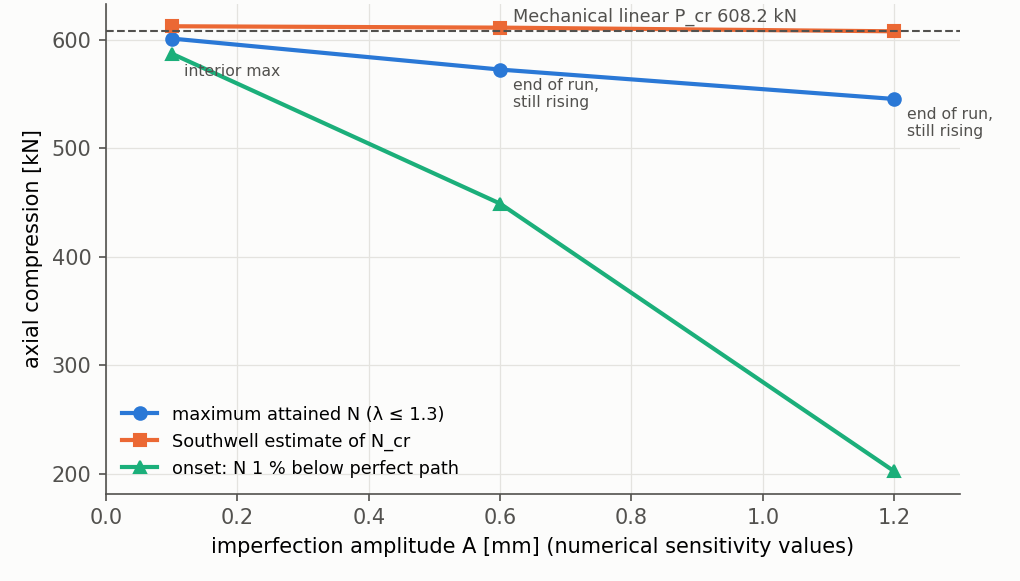
\includegraphics[width=0.62\linewidth,keepaspectratio]{LSD_amplitude_vs_characteristic_load_nt.png}\caption{Imperfection amplitude against maximum attained load, Southwell estimate and onset load}\end{subfigure}
\caption[Mechanical linear buckling against the additional LS-DYNA nonlinear analysis]{Mechanical linear buckling against the additional
LS-DYNA nonlinear analysis. In (a), 8A denotes the Mechanical linear buckling result of Chapter~\ref{ch:buckling} and 12B G6 the LS-DYNA linear
buckling verification run. Load values are not factors of safety.}
\label{fig:lsdcomp}
\src{Plotted with matplotlib from the LS-DYNA solver output of the additional analysis and the Mechanical result (\texttt{MASTER\_PROJECT\_DATA.csv} M099); title strips cropped.}
\end{figure}

\begin{figure}[htbp]
\centering
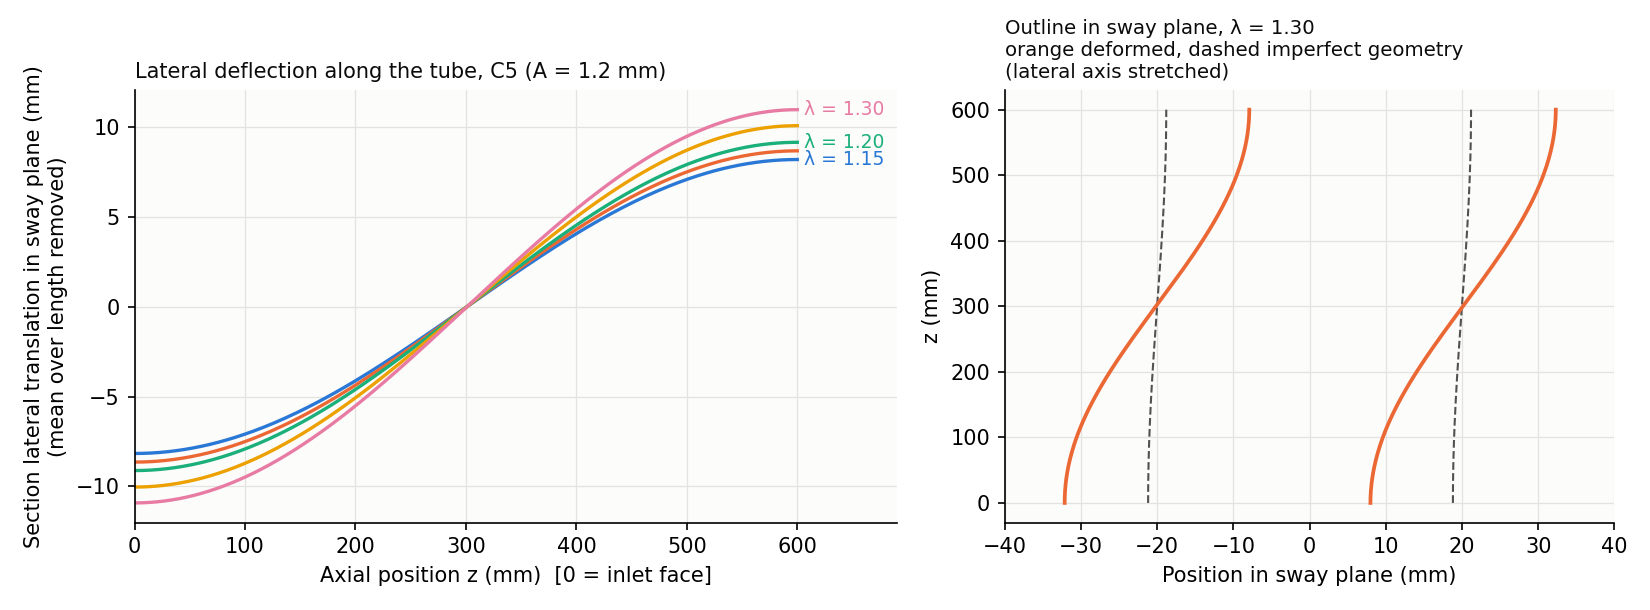
\includegraphics[width=\linewidth,keepaspectratio]{LSD_deformed_shape_C5_nt.png}
\caption[Additional LS-DYNA analysis: deformed shape of the 1.2~mm case]{Additional LS-DYNA analysis, case C5 (1.2~mm): lateral deflection
along the duct for $\lambda$ = 1.15--1.30 (left), and the deformed outline at $\lambda$ = 1.30 against the imperfect geometry (right, lateral
axis stretched). Global guided sway, with the ends moving in opposite directions.}
\label{fig:lsdshape}
\src{Plotted with matplotlib from the LS-DYNA d3plot output of the additional analysis; title strip cropped.}
\end{figure}

\subsection{Limitations of the Elastic Model}
The LS-DYNA model uses elastic, temperature-dependent material behaviour. The project contains no defensible temperature-dependent plastic
stress--strain curve for Inconel~718 (task T-036), so the analysis is not elastic--plastic and does not predict post-yield or collapse
behaviour.

\begin{itemize}
\item \textbf{Yield is reached within the load range.} The peak von Mises stress reaches the local yield estimate at $\lambda$ = 1.109
      (C1), 1.031 (C3) and 0.974 (C5). C5 slightly exceeds the yield estimate before $\lambda$ = 1, and all three cases reach yield during
      the extended loading range.
\item \textbf{Consequences.} The later portions of the load paths lie outside the validated elastic constitutive range. The stresses
      computed there are not physical, and no part of the extended response is a collapse load. The Southwell characteristic-load
      comparison, which uses the pre-critical branches, is the meaningful result.
\item \textbf{Other limitations.}
      \begin{itemize}
      \item The imperfection amplitudes are numerical rather than measured.
      \item Only three amplitudes were analysed.
      \item No mesh-refinement or load-step study was made for the nonlinear response.
      \item The end restraint remains the idealised S1 condition discussed above.
      \end{itemize}
\end{itemize}
\FloatBarrier

% ===================================================================== Chapter 15
\chapter{Parametric Study}\label{ch:param}

\section{Study Design}
The parametric study asks how the flow, thermal and structural responses change with the two operating variables and one design variable
(Table~\ref{tab:pmatrix}). It is a one-factor-at-a-time design around P00 with the S1 supports throughout; the support question is treated
separately (Chapter~\ref{ch:supports}). Every case is an actual simulation chain:
\begin{itemize}
\item a converged Fluent CFD solution of its own (Section 9B-1), with the same physics, staging and convergence criteria as P00;
\item mapping of its own solid temperature field with the method of Chapter~\ref{ch:mapping};
\item Mechanical LC1 and LC2 solutions and a linear buckling solution on the LC2 pre-stress (Section 9B-2).
\end{itemize}
No screening estimate, uniform temperature or interpolated value enters any result of this chapter. A control case, C00, repeated the whole
pipeline for P00 and reproduced it (LC2 peak within $9.5\times10^{-6}$, $\lambda_1$ within $4.2\times10^{-7}$).

%% generated by gen_tables.py - RE-ANALYSIS 2026
\begin{table}[htbp]
\centering
\footnotesize
\caption{Parametric case matrix (one factor at a time around P00; S1 supports)}
\label{tab:pmatrix}
\begin{tabular}{lll>{\raggedright\arraybackslash}p{0.38\linewidth}}
\toprule
Case & Variable & Value (change) & Held constant / mesh \\
\midrule
P00 & -- & baseline & 159,840 CFD cells; mesh B \\
V01 / V03 & inlet velocity & 21.15 / 25.85 m/s ($\mp$10\,\%) & $q''$, geometry; P00 meshes \\
Q01 / Q03 & outer-wall heat flux & 7200 / 8800 W/m$^2$ ($\mp$10\,\%) & $V$, geometry; P00 meshes \\
T01 / T03 & wall thickness & 8 / 12 mm ($\mp$20\,\%; $D_o$ 36 / 44 mm) & total heat input $Q$ held ($q''$ = 8888.9 / 7272.7 W/m$^2$); new CFD meshes 155,520 / 168,480 cells, FE meshes 89,424 / 127,080 nodes \\
\bottomrule
\end{tabular}
\par\smallskip\parbox{\linewidth}{\footnotesize\raggedright Source: \texttt{PROJECT\_STATE.md} \S17--\S19. Range limits: the 600~K air property table (low $V$, high $q''$) and the 128,000-node licence (thick wall).}
\end{table}


The ranges are limited by the solver data rather than chosen arbitrarily. Lower velocity and higher heat flux raise the air temperature at
the wall; the air property table ends at 600~K, and the $-$10\,\% velocity and +10\,\% heat-flux cases reach 580.4~K and 583.4~K on the air side.
The 12~mm wall is the thickest that a 2~mm radial element size allows under the 128,000-node licence (127,080~nodes).

\section{Velocity Cases}
V01 and V03 change the inlet velocity by $\mp$10\,\% at unchanged heat input. Velocity sets the cooling capacity: at 21.15~m/s the air leaves
7.6~K hotter, the maximum solid temperature rises by 24.9~K and the solid mean by 21.5~K; at 25.85~m/s the changes are $-$6.2~K, $-$20.5~K and
$-$17.7~K. The pressure drop changes by $-$13.3 and +14.1\,\% (Figure~\ref{fig:pv}a), a local exponent of about 1.37, lower than the
1.75--2 of isothermal turbulent flow because part of the static pressure drop accelerates the heated air, and that part grows when the air
heats more.

\begin{figure}[htbp]
\centering
\begin{subfigure}[t]{0.325\linewidth}\centering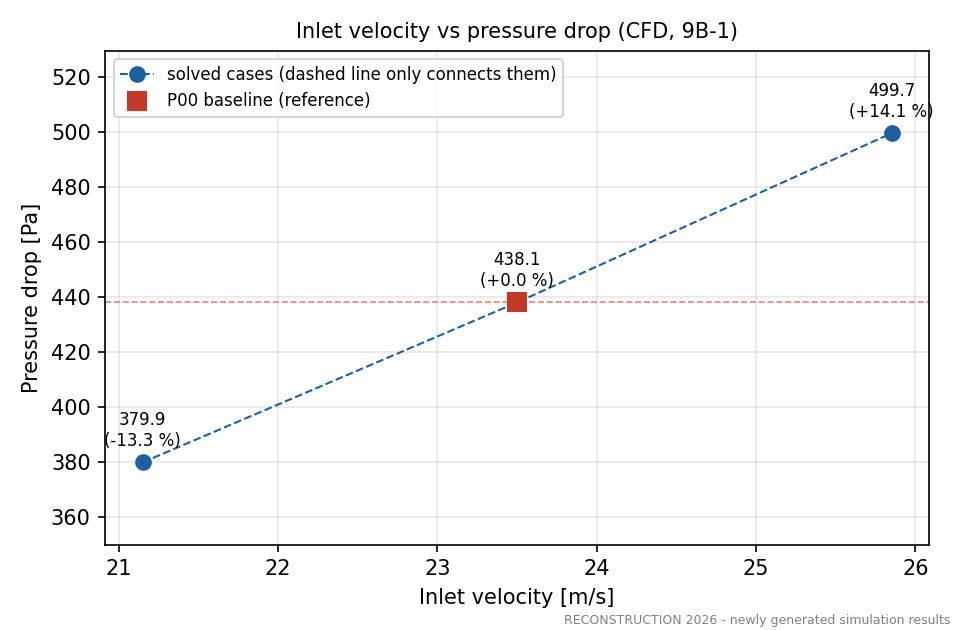
\includegraphics[width=\linewidth]{F01_V_vs_pressure_drop.png}\caption{Pressure drop}\end{subfigure}\hfill
\begin{subfigure}[t]{0.325\linewidth}\centering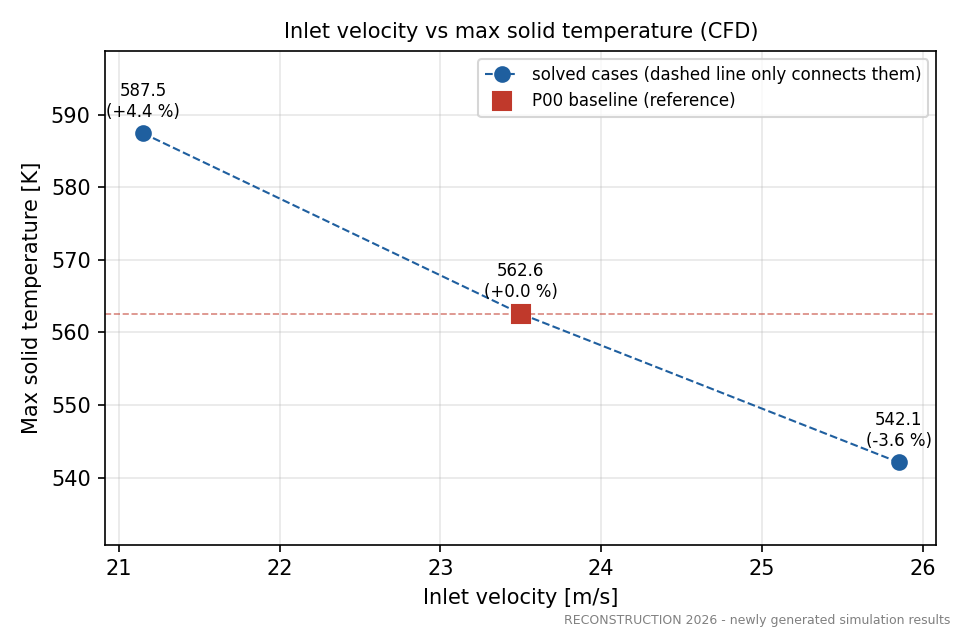
\includegraphics[width=\linewidth]{F03_V_vs_max_solid_temperature.png}\caption{Maximum solid temperature}\end{subfigure}\hfill
\begin{subfigure}[t]{0.325\linewidth}\centering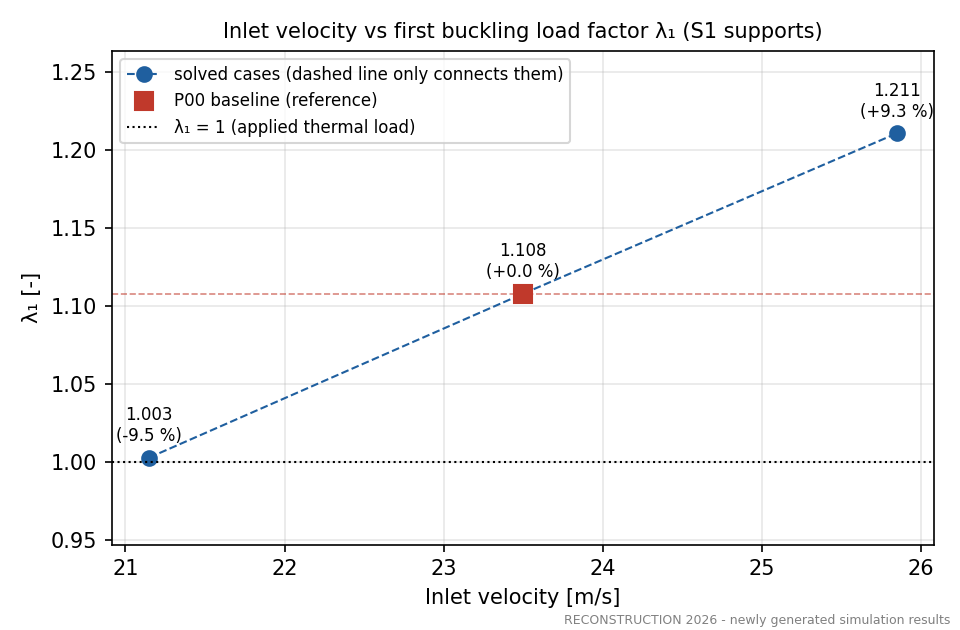
\includegraphics[width=\linewidth]{F05_V_vs_lambda1.png}\caption{First buckling load factor (S1)}\end{subfigure}
\caption[Effect of inlet velocity (21.15, 23.5, 25.85~m/s)]{Effect of inlet velocity (21.15, 23.5, 25.85~m/s); the dashed line only connects the three solved cases.}
\label{fig:pv}
\src{\provdata}
\end{figure}

\section{Heat-Flux Cases}
Q01 and Q03 change the outer-wall heat flux by $\mp$10\,\%. The heat flux is the thermal load itself: the maximum solid temperature changes by
$-$28.1 and +28.6~K and the outlet temperature by $\mp$6.9~K (Figure~\ref{fig:pq}). The solid-mean temperature rise above the inlet changes by
$-$10.8 and +11.0\,\%, slightly more than in proportion; the cause (temperature-dependent air and Inconel properties are a plausible
explanation) was not isolated. The pressure drop changes by only $\pm$4.2\,\%, through the air temperature.

\begin{figure}[htbp]
\centering
\begin{subfigure}[t]{0.325\linewidth}\centering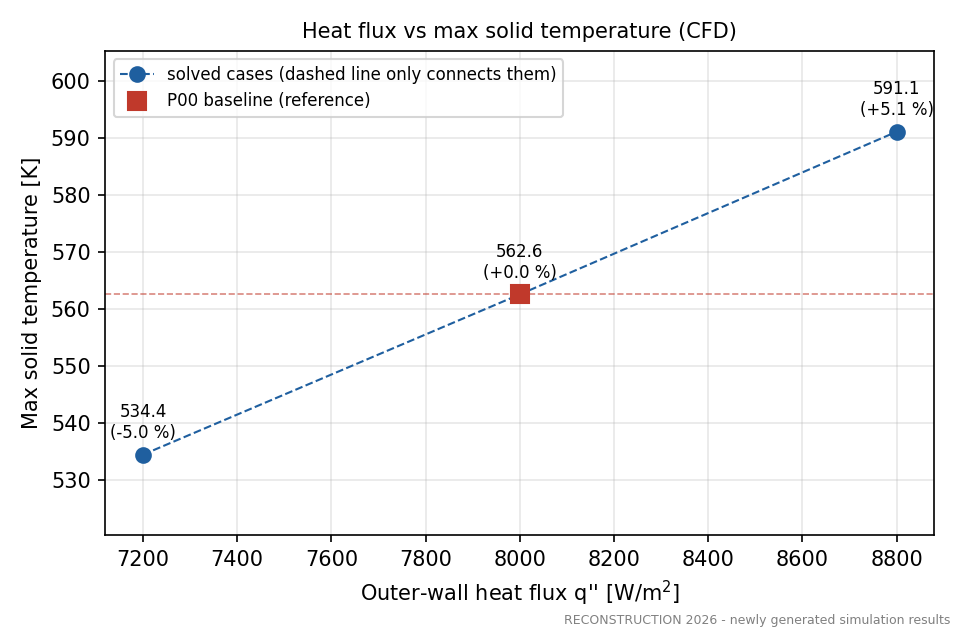
\includegraphics[width=\linewidth]{F07_q_vs_max_solid_temperature.png}\caption{Maximum solid temperature}\end{subfigure}\hfill
\begin{subfigure}[t]{0.325\linewidth}\centering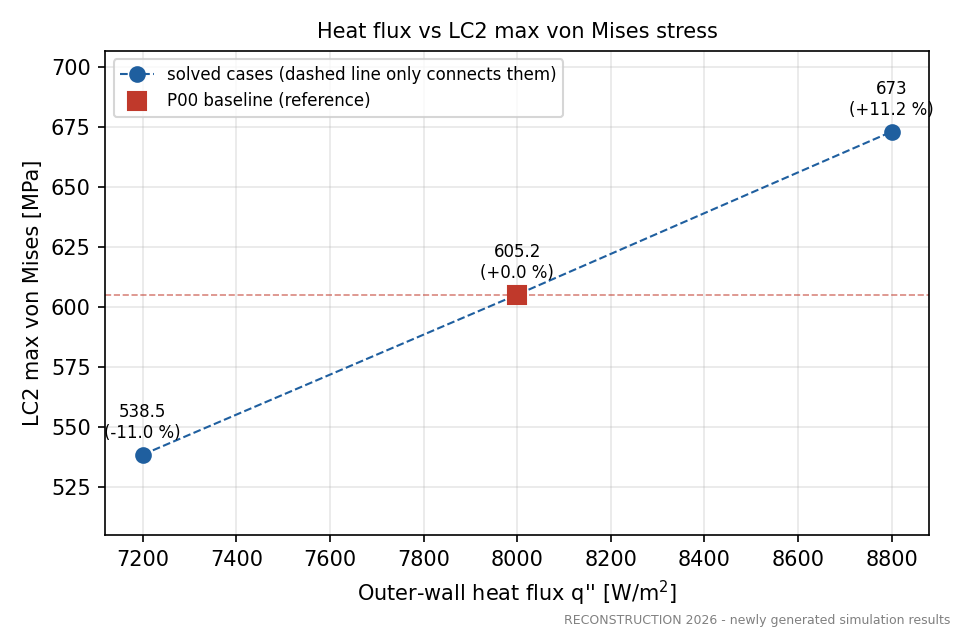
\includegraphics[width=\linewidth]{F08_q_vs_LC2_stress.png}\caption{LC2 maximum von Mises stress}\end{subfigure}\hfill
\begin{subfigure}[t]{0.325\linewidth}\centering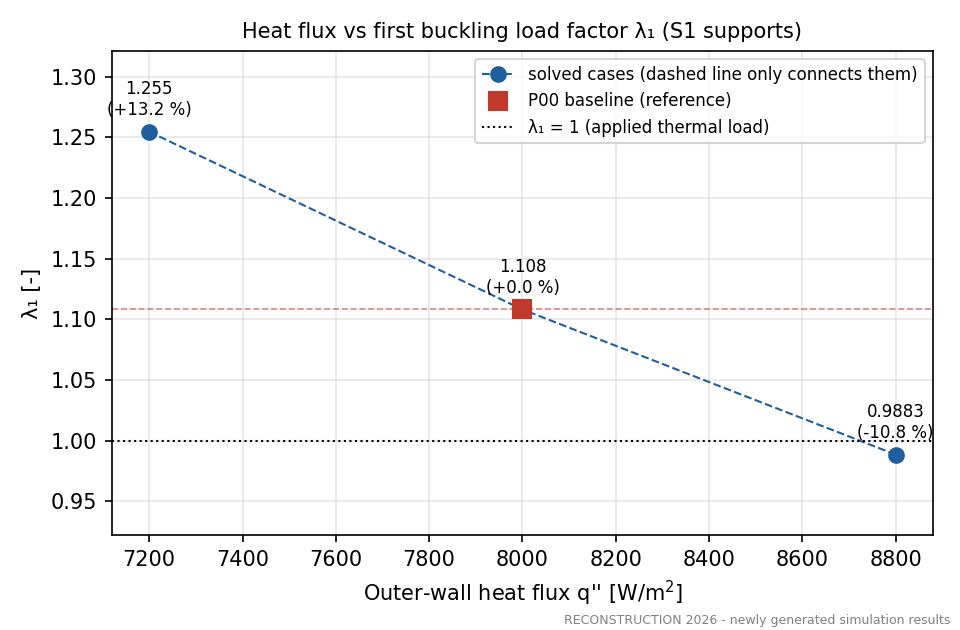
\includegraphics[width=\linewidth]{F09_q_vs_lambda1.png}\caption{First buckling load factor (S1)}\end{subfigure}
\caption{Effect of outer-wall heat flux (7200, 8000, 8800~W/m$^2$).}
\label{fig:pq}
\src{\provdata}
\end{figure}

\section{Wall-Thickness Cases}
T01 and T03 change the wall thickness to 8 and 12~mm (outer diameter 36 and 44~mm) with the bore unchanged. To isolate the section effect,
the total heat input is held at the baseline value, so the outer-wall flux becomes 8888.9 and 7272.7~W/m$^2$. New CAD models, CFD meshes
(9 and 12 solid layers) and structural meshes (four and six 2.0~mm elements through the wall) were built. The outlet temperature and pressure drop are unchanged,
and the solid temperatures move by less than 1~K: the through-wall temperature difference (6.44 / 7.58 / 8.61~K for 8 / 10 / 12~mm) and the
axial conduction through the changed cross-section act in opposite directions. A check solution of T03 with 18 instead of 12 solid layers
changed the node temperatures by at most 0.197~K.


\section{CFD Results}
Table~\ref{tab:pcfd} lists the CFD results. Every case converged at iteration 600 and held at 700, with mass and energy imbalances of at most
$4.2\times10^{-14}$ and $1.3\times10^{-12}$, $y^+_{max}$ between 0.524 and 0.645, and all temperatures inside the property tables. An independent
verification script re-derived the CFD results from the raw case outputs (309 of 309 checks passed).

%% generated by gen_tables.py - RE-ANALYSIS 2026
\begin{table}[htbp]
\centering
\footnotesize
\caption{Parametric CFD results (actual Fluent solutions, 9B-1)}
\label{tab:pcfd}
\begin{tabular}{lrrrrrrr}
\toprule
Case & $\Delta p$ [Pa] & $T_{out}$ [K] & $T_{max}$ [K] & $Q$ [W] & $Re_{in}$ & $T_{int,max}$ [K] & $\bar T_s$ [K] \\
\midrule
P00 & 438.13 & 368.93 & 562.58 & 602.76 & 29,958 & 555.27 & 525.48 \\
V01 & 379.93 & 376.56 & 587.47 & 602.76 & 26,962 & 580.38 & 546.96 \\
V03 & 499.69 & 362.69 & 542.10 & 602.76 & 32,954 & 534.61 & 507.78 \\
Q01 & 419.74 & 362.06 & 534.45 & 542.48 & 29,958 & 527.65 & 501.07 \\
Q03 & 456.64 & 375.79 & 591.13 & 663.03 & 29,958 & 583.35 & 550.31 \\
T01 & 438.11 & 368.93 & 561.97 & 602.76 & 29,958 & 555.76 & 524.54 \\
T03 & 438.14 & 368.93 & 563.07 & 602.76 & 29,958 & 554.78 & 526.38 \\
\bottomrule
\end{tabular}
\par\smallskip\parbox{\linewidth}{\footnotesize\raggedright Source: \texttt{MASTER\_PROJECT\_DATA.csv} ($\Delta p$, $T_{out}$, $T_{max}$: VERIFIED); $Q$, $Re_{in}$, interface maximum $T_{int,max}$ and solid mean $\bar T_s$ from \texttt{10\_Parametric\_Study/CFD\_Results/PARAMETRIC\_CFD\_TABLE.md} and \texttt{PROJECT\_STATE.md} \S18.3.}
\end{table}


\section{Structural Results}
The static structural results are given in Table~\ref{tab:pstruct}. For velocity and heat flux, every structural response follows the change
of the wall temperature: the LC1 growth, the LC2 end force, the LC2 stresses and the utilisation all change with normalised sensitivities
between 0.87 and 1.20 in magnitude. The LC2 peak von Mises stress changes slightly less than the mean axial stress (for V01 +9.56\,\% against
+9.72\,\%), because the temperature at the critical inlet-edge node changes less than the duct mean. For thickness the stress level barely
changes (LC2 peak $-$0.47 / +0.43\,\%), while the end force scales with the section area ($-$25.6 / +28.5\,\%). The critical locations do not move
in any case: LC2 at the outer edge of the inlet face, LC1 at the bore 6.5~mm from the inlet. No case is yield-limited; the highest
utilisation is 0.6446 (Q03).

%% generated by gen_tables.py - RE-ANALYSIS 2026
\begin{table}[htbp]
\centering
\footnotesize
\caption{Parametric static structural results (actual Mechanical solutions, 9B-2; S1 supports)}
\label{tab:pstruct}
\begin{tabular}{lrrrrrrrr}
\toprule
Case & LC1 def.\ [mm] & $\Delta L$ [mm] & LC1 VM [MPa] & LC2 VM [MPa] & $\bar\sigma_z$ [MPa] & $T_{crit}$ [K] & $S_y(T)$ [MPa] & Util. \\
\midrule
P00 & 1.8443 & 1.8409 & 24.282 & 605.161 & $-$582.440 & 437.99 & 1047.0 & 0.5780 \\
V01 & 2.0375 & 2.0339 & 24.925 & 663.001 & $-$639.053 & 450.38 & 1044.6 & 0.6347 \\
V03 & 1.6874 & 1.6842 & 23.532 & 557.544 & $-$535.853 & 427.76 & 1049.1 & 0.5315 \\
Q01 & 1.6284 & 1.6253 & 21.704 & 538.526 & $-$518.230 & 423.38 & 1050.0 & 0.5129 \\
Q03 & 2.0680 & 2.0641 & 26.649 & 673.024 & $-$647.830 & 452.79 & 1044.1 & 0.6446 \\
T01 & 1.8355 & 1.8328 & 20.872 & 602.309 & $-$580.048 & 429.52 & 1048.7 & 0.5743 \\
T03 & 1.8528 & 1.8487 & 27.206 & 607.735 & $-$584.750 & 445.36 & 1045.6 & 0.5813 \\
\bottomrule
\end{tabular}
\par\smallskip\parbox{\linewidth}{\footnotesize\raggedright Source: \texttt{MASTER\_PROJECT\_DATA.csv} (LC1 deformation, LC1/LC2 von Mises, utilisation: VERIFIED); $\Delta L$, mean axial stress $\bar\sigma_z$, critical temperature and local $S_y$ from \texttt{10\_Parametric\_Study/Results/PARAMETRIC\_STRUCTURAL\_RESULTS.csv}.}
\end{table}


\section{Buckling Results}
Table~\ref{tab:pbk} gives the buckling results. The mode is the global guided-sway shape in every case. Velocity and heat flux change
$\lambda_1$ through the end force, with the critical load itself almost constant ($P_{cr}$ changes by less than 0.8\,\%) because the section and
the modulus change little. Thickness changes $\lambda_1$ through the section: $P_{cr}$ scales with the bending stiffness ($-$36.6 / +49.3\,\%),
the end force with the area, and $\lambda_1 \propto I/(A\,\varepsilon_{th}) \propto r_g^2$, so the thin wall loses and the thick wall gains
stability margin in the idealised sense (Figure~\ref{fig:pt}).

Under S1, $\lambda_1$ falls below 1 for \textbf{Q03} (0.98834) and \textbf{T01} (0.94497). For these two cases the LC2 static stresses are
idealised pre-buckling equilibrium results: the linear stability criterion indicates loss of stability before the applied load level, and
they are not presented as physically stable operating states. \textbf{V01} ($\lambda_1$ = 1.00307) lies 0.31\,\% above 1, extremely close to the
limit; its side of 1 is inside the thermal and material uncertainty bands. In all seven S1 cases $\lambda_1$ is below the first-yield factor, so
every case is stability-first in the idealised model.

\begin{figure}[htbp]
\centering
\begin{subfigure}[t]{0.325\linewidth}\centering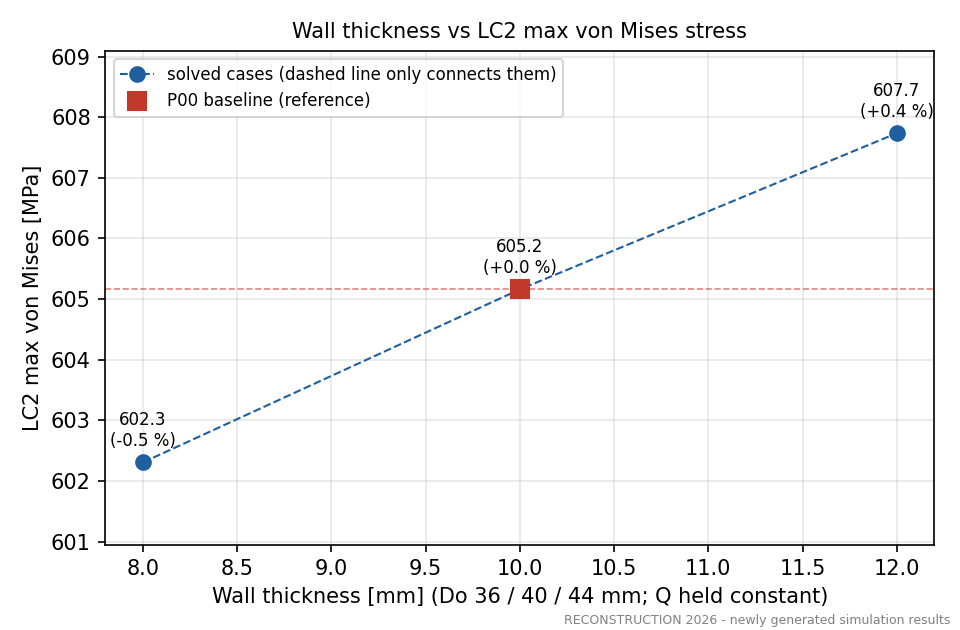
\includegraphics[width=\linewidth]{F11_t_vs_LC2_stress.png}\caption{LC2 maximum von Mises stress}\end{subfigure}\hfill
\begin{subfigure}[t]{0.325\linewidth}\centering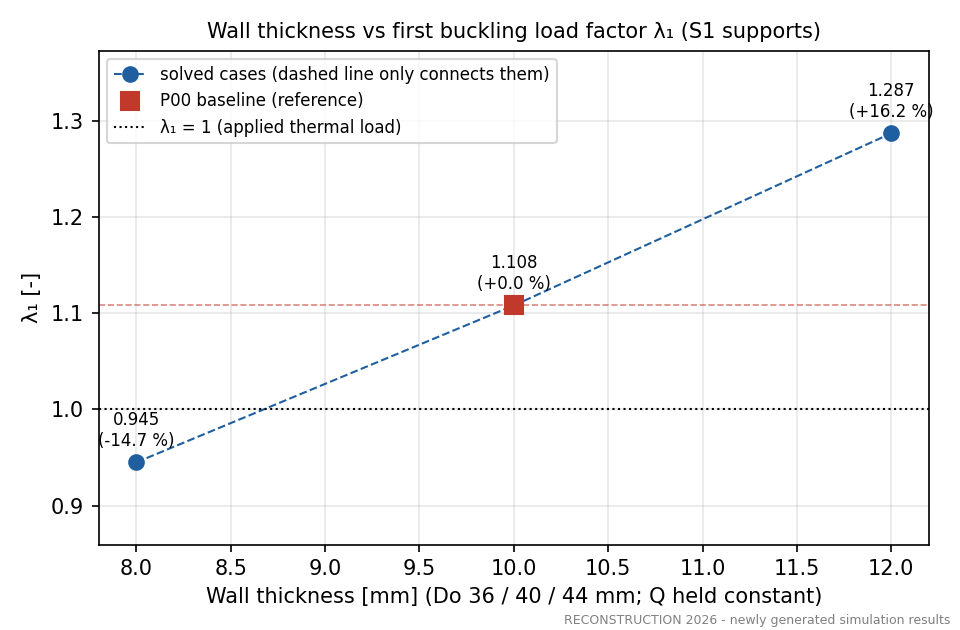
\includegraphics[width=\linewidth]{F12_t_vs_lambda1.png}\caption{First buckling load factor (S1)}\end{subfigure}\hfill
\begin{subfigure}[t]{0.325\linewidth}\centering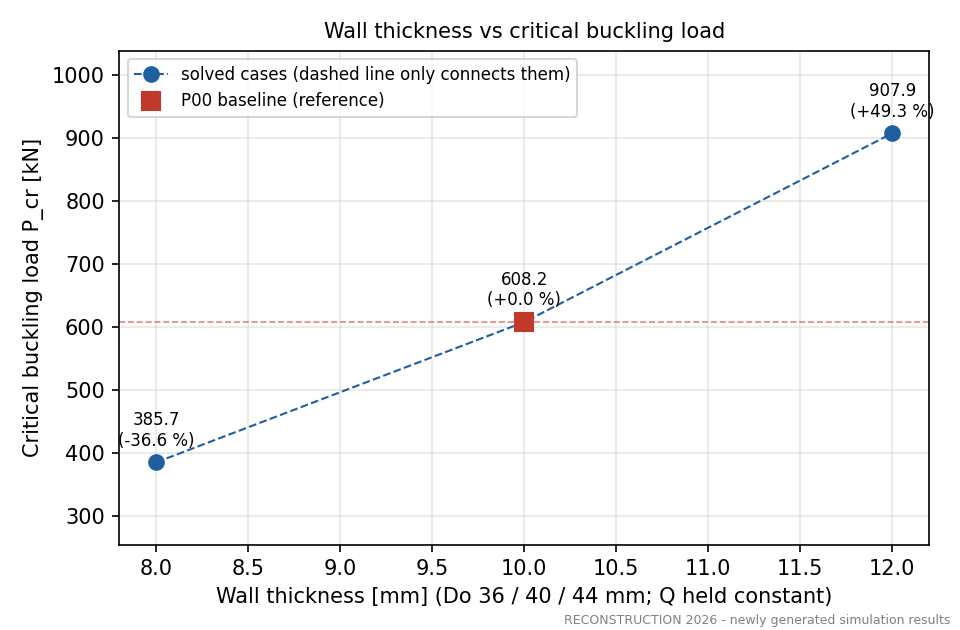
\includegraphics[width=\linewidth]{F13_t_vs_critical_buckling_load.png}\caption{Critical buckling load}\end{subfigure}
\caption{Effect of wall thickness (8, 10, 12~mm) at constant total heat input.}
\label{fig:pt}
\src{\provdata}
\end{figure}

%% generated by gen_tables.py - RE-ANALYSIS 2026
\begin{table}[htbp]
\centering
\footnotesize
\caption{Parametric linear buckling results under S1 (actual eigenvalue solutions, 9B-2)}
\label{tab:pbk}
\begin{tabular}{lrrrrll}
\toprule
Case & $N$ [kN] & $\lambda_1$ & $P_{cr}$ [kN] & First-yield factor & First reached & Note \\
\midrule
P00 & 548.94 & 1.10805 & 608.25 & 1.730 & buckling &  \\
V01 & 602.29 & 1.00307 & 604.14 & 1.575 & buckling & 0.31\,\% above 1 \\
V03 & 505.03 & 1.21087 & 611.53 & 1.882 & buckling &  \\
Q01 & 488.42 & 1.25464 & 612.79 & 1.950 & buckling &  \\
Q03 & 610.57 & 0.98834 & 603.45 & 1.551 & buckling & \textbf{$<$ 1: pre-buckling equilibrium} \\
T01 & 408.19 & 0.94497 & 385.73 & 1.741 & buckling & \textbf{$<$ 1: pre-buckling equilibrium} \\
T03 & 705.43 & 1.28702 & 907.89 & 1.720 & buckling &  \\
\bottomrule
\end{tabular}
\par\smallskip\parbox{\linewidth}{\footnotesize\raggedright Source: \texttt{MASTER\_PROJECT\_DATA.csv} ($\lambda_1$, $P_{cr}$: VERIFIED); end force $N$ and first-yield factor from \texttt{PROJECT\_STATE.md} \S19.3. Mode 1 is the global guided-sway shape in every case. For Q03 and T01 the LC2 static stresses are idealised pre-buckling equilibrium results: the linear stability criterion indicates loss of stability before the applied load level.}
\end{table}


\section{Sensitivity Trends}
Table~\ref{tab:psens} compares the three variables through normalised sensitivities, which remove the different step sizes. Velocity acts
most strongly on the pressure drop ($S$ = +1.37); heat flux most strongly on $\lambda_1$ ($S = -1.20$) and on the thermal growth; thickness most
strongly on the critical load ($S$ = +2.15) and the end force, with a negligible effect on temperatures ($|S| \le 0.009$). The normalised effect
of thickness on $\lambda_1$ (+0.77) is of the same order as those of velocity (+0.94) and heat flux ($-$1.20), although it acts through a
different mechanism. The 9A analytical screening, prepared before the simulations, agreed with the FE values of $\lambda_1$ to within
0.78\,\%, but placed V01 at or below 1; the FE result (1.0031) supersedes it, and no conclusion of this report uses a screening value.

%% generated by gen_tables.py - RE-ANALYSIS 2026
\begin{table}[htbp]
\centering
\footnotesize
\caption{Normalised sensitivities $S = (\Delta y/y_0)/(\Delta x/x_0)$ from the one-factor steps}
\label{tab:psens}
\begin{tabular}{lrrr}
\toprule
Response $y$ & Velocity $V$ & Heat flux $q''$ & Thickness $t$ \\
\midrule
Pressure drop $\Delta p$ & +1.367 & +0.421 & $\approx 0$ \\
Maximum solid temperature & $-$0.403 & +0.504 & +0.005 \\
LC1 axial growth & $-$0.950 & +1.192 & +0.022 \\
LC2 max von Mises & $-$0.871 & +1.111 & +0.022 \\
LC2 end reaction & $-$0.886 & +1.113 & +1.354 \\
$\lambda_1$ & +0.938 & $-$1.202 & +0.772 \\
$P_{cr}$ & +0.061 & $-$0.077 & +2.146 \\
\bottomrule
\end{tabular}
\par\smallskip\parbox{\linewidth}{\footnotesize\raggedright Source: \texttt{10\_Parametric\_Study/Results/PARAMETRIC\_TRENDS.md} (central differences over the low/high cases). Families are compared only through $S$, because the step sizes differ ($\pm$10\,\% for $V$ and $q''$, $\pm$20\,\% for $t$).}
\end{table}


\section{Limitations of One-Factor-at-a-Time Analysis}
The design varies one parameter at a time about P00. It cannot identify interactions: the screening estimated the velocity $\times$ heat-flux
interaction at about 8--11\,\% of the main effects, so combined off-baseline states (for example low velocity and high heat flux together) cannot
be obtained by adding the one-factor changes. The mid-point deviation from linearity describes curvature along one axis only. No response
surface was fitted and nothing is extrapolated beyond the $\pm$10\,\% ($V$, $q''$) and $\pm$20\,\% ($t$) steps.

% ===================================================================== Chapter 16
\chapter{Uncertainty and Limitations}\label{ch:unc}
Nine sources of uncertainty were identified and are kept separate (Table~\ref{tab:unc}). They are of different kinds -- discretisation
errors, model-form and idealisation errors, data scatter and assumptions -- several have a known sign and some are not quantified. A combined
uncertainty percentage would therefore have no mathematical basis and is not formed. The evidence supports the ranking primary (end restraint
and stability modelling) $\gg$ secondary (thermal field and material data) $\gg$ smaller (mapping, structural mesh, Poisson's ratio).

%% generated by gen_tables.py - RE-ANALYSIS 2026
\begin{table}[htbp]
\centering
\footnotesize
\caption{Uncertainty register: nine separate sources (no combined percentage is formed)}
\label{tab:unc}
\begin{tabular}{l>{\raggedright\arraybackslash}p{0.20\linewidth}>{\raggedright\arraybackslash}p{0.50\linewidth}>{\raggedright\arraybackslash}p{0.11\linewidth}}
\toprule
\# & Source & Size / evidence & Class \\
\midrule
7 & End-restraint definition & $\lambda_1$ = 1.108 / 2.232 / 4.300 (S1 / S3 / S2) at identical static stress: factor 3.9; mechanism switches & primary \\
8 & Geometric imperfection & not modelled in the Mechanical study (numerical amplitudes only in the additional elastic LS-DYNA analysis, Section~\ref{sec:lsdyna}); reduces real capacity below $\lambda_1$ by an unknown amount & primary \\
9 & Inelastic buckling & intermediate columns ($KL/r$ 49.7--58.3 $<$ $C_c \approx$ 60); Johnson estimate 1.058 for S1 & primary \\
2 & CFD model form & not quantified; 19.1 K CFD--analytical gap on $T_{max}$; $\approx$30 K on the mean rise; $\lambda_1 \approx$ 0.98 on the Section 2 temperature basis & secondary \\
1 & CFD mesh & $T_{max}$ $-$5.1 / +1.6 K; LC2 stress $-$10.1 / +2.8 MPa; $\lambda_1$ +1.8 / $-$0.5\,\% & secondary \\
5 & Material data & about $\pm$2\,\% on $E$ and $\alpha$; $S_y$ typical values & secondary \\
3 & Temperature mapping & $\le$ 0.081 K interior; LC1 inlet peak bound $\pm$9.8 MPa & smaller \\
4 & Structural mesh & LC2 peak $\le 4.9\times10^{-4}$, $\lambda_1 \le 5.4\times10^{-5}$; LC1 bore $-$2.1\,\% & smaller \\
6 & Poisson's ratio & about 1.4\,\% on LC1; none on LC2 & smaller \\
\bottomrule
\end{tabular}
\par\smallskip\parbox{\linewidth}{\footnotesize\raggedright Source: \texttt{11\_Final\_Audit/MASTER\_UNCERTAINTIES.md}. Sources are of different kind and sign (discretisation, model form, data scatter, assumption); a root-sum-square or linear sum would have no mathematical basis.}
\end{table}


\section{Data-Availability Limitation}
The original internship files were not retained, so no result can be compared with the analysis made during the internship, and nothing
in this report is a recovered value. The analysed problem is representative of the internship problem, not a reproduction of it.

\section{CFD Model Form}
The turbulence and property models were not varied. Indicators of the model-form uncertainty are the 9\,\% difference between the CFD Nusselt
number and the property-corrected correlation, the 10.4\,\% difference in friction factor (mostly a gas-heating effect, about five points
unexplained), the 19.1~K difference in maximum solid temperature from the analytical model and the difference of about 30~K in mean
temperature rise. The last one matters structurally: on the Section 2 temperature basis the S1 buckling factor would be about 0.98 instead of
1.108. Uniform heating, neglected radiation and the assumed inlet turbulence intensity add further, unquantified, model-form uncertainty.

\section{CFD Mesh}
The medium mesh is approximately convergent. Its band against the extrapolated solution is $-$5.1 / +1.6~K on the maximum solid temperature, which
propagates to $-$10.1 / +2.8~MPa on the LC2 stress, $-$13.7 / +4.3~MPa on the local peak, +1.8 / $-$0.5\,\% on $\lambda_1$ and $-$32 / +9~\textmu m on
the free growth. The medium field is slightly hot, so the structural results lean conservative.

\section{Temperature Mapping}
The transfer error is at most 0.081~K inside the source mesh. Within about 11~mm of the inlet the source node values carry the Fluent
reconstruction limitation of up to 2.6~K, which bounds the LC1 inlet peak at $\pm$9.8~MPa and the LC2 peak at 1.6\,\%. The re-numbering of source
nodes between otherwise identical cases changes the mapped field by at most 0.081~K and the LC2 peak by $9.5\times10^{-6}$.

\section{Structural Mesh}
The governing LC2 results and $\lambda_1$ change by at most $4.9\times10^{-4}$ and $5.4\times10^{-5}$ across seven meshes. The LC1 mid-span bore
stress is under-predicted by 2.1\,\% on mesh B (sign known). On one thickness check mesh the LC2 inlet-edge peak changed by $1.4\times10^{-4}$,
above the $10^{-4}$ class-A tolerance at a single node; this was reported, not relaxed.

\section{Material Data}
The properties are generic datasheet values, not lot-specific. An uncertainty of about $\pm$2\,\% on $E$ and $\alpha$ acts directly on the
restrained stress and end force ($\propto E\alpha$). The yield strengths are typical rather than minimum-guaranteed values, so the utilisation
is not a certified margin. No temperature-dependent stress--strain curve is available.

\section{Poisson's Ratio}
$\nu$ = 0.294 is assumed; the literature range is 0.284--0.294. It affects the LC1 radial and hoop stresses by about 1.4\,\% and the uniaxial LC2
axial stress not at all; $\lambda_1$ is affected only through the shear correction.

\section{End Restraint}
The real flange stiffness is undefined. The idealised supports change $\lambda_1$ from 1.108 (S1) to 2.232 (S3) and 4.300 (S2) at identical
static stress and switch the governing mechanism from bifurcation-first to first-yield-first. Rotational flexibility would lower $\lambda_1$ below
S1. This is the primary uncertainty of every stability statement in the report.

\section{Geometric Imperfections}
The tube is modelled perfectly straight, without out-of-straightness, eccentricity of the end load or residual stress. A real tube deflects
laterally below the bifurcation load and its capacity is lower; the size of the reduction is unknown without an imperfection-sensitive
nonlinear analysis. The additional LS-DYNA analysis (Section~\ref{sec:lsdyna}) quantifies the elastic response for three numerical imperfection
amplitudes; without measured imperfection data and an inelastic material model, the reduction for a real tube remains unknown.

\section{Inelastic Buckling}
All cases are intermediate columns ($KL/r$ = 49.7--58.3 under S1, below $C_c \approx$ 60) with an elastic buckling stress above the conventional
proportional limit. The linear elastic eigenvalue analysis cannot capture the resulting inelastic reduction; the conventional Johnson factors
(1.058 guided, 1.414 fixed--pinned, 1.581 fixed--fixed) indicate its direction but are not material-specific.

\section{Missing Experimental Validation}
No measured data exist. The CFD is verified against conservation laws, correlations and mesh studies, and the structural model against
closed-form solutions and equilibrium checks, but neither is validated against experiment. Agreement with correlations shows consistency,
not accuracy with respect to a physical duct.

\section{Interaction Effects}
The parametric study is one factor at a time over a narrow envelope ($\pm$10\,\% in velocity and heat flux, $\pm$20\,\% in thickness). Interactions
of about 8--11\,\% of the main effects were estimated for velocity and heat flux but not simulated. Transient start-up, thermal cycling and
fatigue are outside the scope.

% ===================================================================== Chapter 17
\chapter{Engineering Discussion}\label{ch:discussion}

\section{Flow Behavior}
The flow is a developing turbulent pipe flow with strong heating. Two features distinguish it from a textbook isothermal case. First, the
air density falls by about a fifth along the duct, so the flow accelerates and a third of the static pressure drop (149~Pa of 438~Pa) goes into
acceleration rather than friction. Second, heating lowers the wall friction relative to the constant-property correlation by about 9\,\%. The
second effect explains why the friction factor misses the Petukhov value by slightly more than 10\,\%, and it is a property of the physics, not
of the mesh. For the structural question, the flow matters mainly through the heat-transfer coefficient it produces.

\section{Thermal Behavior}
The thermal behaviour is controlled by the air-side film. The metal carries only a few percent of the thermal resistance, so the wall is
almost isothermal through its thickness (7.6~K across 10~mm at mid-span) but runs about 186~K above the bulk air near the outlet. Along the duct
the wall temperature follows the bulk temperature plus the film temperature difference, modified at both ends by conduction: the inlet end is
cooled by the high heat-transfer coefficient of the thermal entrance, which draws heat axially through the wall, and the outlet end is
warmed by the adiabatic end face. This is why the CFD maximum is 19~K below the one-dimensional estimate and why the mean temperature rise, which
drives the structural loads, is about 11\,\% lower than in the analytical model. The conjugate CFD was therefore necessary: the one-dimensional
model overestimates the structural loads because it cannot represent the entrance and end effects.

\section{Structural Behavior}
The structural behaviour is governed by restraint rather than by the gradient. Free expansion produces a growth of 1.84~mm but only 24~MPa of
stress, confined to the inlet end; restrained expansion stores the same strain as a nearly uniform compression of 582~MPa. The thermal
problem therefore translates into a restraint problem: the stress level depends on how much of the growth the mounting prevents, not on
the temperature distribution within the wall. The static state is elastic in every case, with the peak at the inlet-face edge where the
compression and the inlet gradient combine.

\section{Buckling Behavior}
The restrained duct is a stocky column carrying a thermal, displacement-controlled load close to its idealised Euler load. Under S1 the first
bifurcation appears at 1.108 times the applied load, before first yield. Two points qualify this result. The load is thermal, so a small
change in mean temperature (about 24~K) changes the load factor by the full 10.8\,\%; the stability statement is therefore as uncertain as the
mean wall temperature, which itself differs by 30~K between the analytical and CFD models. And the linear eigenvalue is an upper-bound-type
indicator for a perfect column; imperfections and inelastic behaviour act only to lower the real capacity. The additional LS-DYNA
analysis (Section~\ref{sec:lsdyna}) is consistent with this: with mode-shaped imperfections the lateral deflection and stress grow well below
$\lambda_1$, while the Southwell characteristic-load estimates stay within 1\,\% of the linear critical load.

\section{Effect of Velocity}
Velocity primarily affects cooling, Reynolds number and pressure drop. It changes the heat-transfer coefficient and the air temperature rise,
and through them the wall temperature; the structural response then follows the temperature. A 10\,\% lower velocity raises the wall
temperatures by about 25~K, the restrained force by 9.7\,\% and lowers $\lambda_1$ to 1.003, while the critical load itself hardly changes. The
pressure-drop penalty of higher velocity (+14.1\,\% for +10\,\% velocity) is the price of the cooler wall.

\section{Effect of Heat Flux}
Heat flux directly drives temperature and thermal stress. It acts on the wall temperature rise almost in proportion (slightly more than
proportionally), and every thermal-structural response follows: $\pm$10\,\% flux gives about $\pm$11\,\% restrained force and LC2 stress and moves
$\lambda_1$ from 1.255 to 0.988. It is the variable to which $\lambda_1$ is most sensitive. The pressure drop changes only through the gas
temperature.

\section{Effect of Wall Thickness}
Wall thickness strongly affects stiffness and buckling capacity while having relatively little thermal effect under the constant-total-heat-input
definition. Temperatures change by less than 1~K and the stress level by less than 0.5\,\%, but the end force scales with the area and the
critical load with the bending stiffness. A thicker wall carries a larger force but gains more capacity, because the radius of gyration
grows; a thinner wall loses capacity faster than it loses force. Thickness is therefore a structural design variable, not a thermal one, in
this range. With the heat flux held constant instead of the total heat input, the thermal effect would differ; that alternative was not studied.

\section{Effect of Support Condition}
The support condition dominates the idealised buckling factor. With identical static stress, the three idealised supports change $\lambda_1$ by
a factor of 3.9, far more than any operating or design variable in the study, and they decide whether bifurcation or first yield is reached
first. The mesh resolution, by comparison, changes $\lambda_1$ by less than $10^{-4}$ on the structural side and by up to about 2\,\% through the
CFD temperature field. The mesh is not the dominant uncertainty; the boundary condition is.

\section{Physical Interpretation}
Taken together, the results describe a chain in which each link amplifies the importance of the next. The air film sets the wall
temperature; the restraint converts that temperature into a large compressive force; and the end fixity decides whether that force is
stable. Pressure loading is negligible throughout ($7.4\times10^{-6}$\,\% of the peak stress). The engineering implication, within the
idealised model, is that the design question for such a duct is less about reducing the through-wall gradient than about how
much axial growth the mounting prevents and how the ends are restrained laterally and rotationally. Allowing controlled axial growth, or
providing defined lateral end restraint, are the two routes the model identifies; neither was analysed as a design and both would need the
real mounting to be defined.

% ===================================================================== Chapter 18
\chapter{Conclusions}\label{ch:conclusions}
The following conclusions apply within the idealised numerical model; they are simulation results that have not been
validated against measurement.

\begin{enumerate}
\item \textbf{CFD.} The baseline Fluent solution of the heated duct is converged (iteration 600, confirmed at 700) and conserves mass and
      energy to $7.0\times10^{-13}$\,\% and $3.1\times10^{-11}$\,\%. The wall is resolved ($y^+ \le$ 0.585). The pressure drop is 438.13~Pa, the
      fully developed Nusselt number 54.17 and the friction factor 0.02163, 10.4\,\% below Petukhov, mainly because of gas heating.
\item \textbf{Mesh independence.} The three-mesh study, with the polygon-faceting effect separated exactly, shows approximately convergent
      behaviour (apparent order 1.2--1.6). The medium mesh is 4.4~K hotter than the extrapolated solution at the maximum solid temperature; its
      error is small and conservative for the structural phase. Strict mesh independence is not claimed.
\item \textbf{Thermal field.} The air film carries most of the thermal resistance. The maximum solid temperature is 562.58~K on the medium mesh (fine mesh
      560.83~K, extrapolated 558.13~K) against 581.7~K in the one-dimensional analytical model; the through-wall temperature difference is only
      7.58~K at mid-span.
\item \textbf{Structural response.} Free expansion gives 1.8443~mm of maximum deformation and a 24.28~MPa peak von Mises stress. Full axial
      restraint gives an end force of 548.94~kN, a mean axial stress of $-$582.44~MPa and a local peak von Mises stress of 605.16~MPa,
      57.8\,\% of the local yield strength. Restraint, not the through-wall gradient, dominates the thermal stress (32$\times$ at mid-span).
      The structural results are insensitive to the structural mesh ($\le 4.9\times10^{-4}$) and to the fluid pressure ($7.4\times10^{-6}$\,\%).
\item \textbf{Buckling.} Under the baseline S1 support the linear eigenvalue buckling factor is 1.108, below the first-yield factor of 1.730:
      the idealised S1 model is stability-limited and close to instability. $\lambda_1$ is a linear stability indicator of a perfect elastic
      column, not a collapse load and not a factor of safety.
\item \textbf{Parametric study.} Velocity acts mainly on cooling and pressure drop and on the structure through the temperature; heat flux
      drives temperature and thermal stress directly; wall thickness acts on stiffness and buckling capacity with little thermal effect. Under
      S1, $\lambda_1$ falls below 1 for +10\,\% heat flux (Q03, 0.988) and the 8~mm wall (T01, 0.945); their static stresses are pre-buckling
      equilibrium results. The $-$10\,\% velocity case lies at 1.003.
\item \textbf{Support sensitivity.} The end restraint changes $\lambda_1$ from 1.108 (S1) to 2.232 (S3) and 4.300 (S2) at identical static stress
      and switches the governing mechanism from bifurcation-first to first-yield-first. The supports are the dominant uncertainty of the
      stability conclusion.
\item \textbf{Additional nonlinear LS-DYNA analysis (extension).} With numerical mode-1 imperfections of 0.1, 0.6 and 1.2~mm, the
      Southwell characteristic-load estimates (607.7--612.3~kN) are close to the linear critical load of 608.25~kN: the characteristic
      global buckling load is relatively insensitive to the tested amplitudes, while the onset of lateral deformation, the deflection
      and the stress at a given load are strongly imperfection-sensitive. The model is elastic and first local yield is reached at
      $\lambda$ = 0.974--1.109, so the later parts of the load paths lie outside its validated range. The result is not a real-world
      capacity, a factor of safety or an experimental validation (Section~\ref{sec:lsdyna}).
\item \textbf{Limitations.} The real end restraint and inelastic material behaviour were not modelled, geometric imperfections only as
      numerical amplitudes in the additional elastic LS-DYNA analysis, the CFD model form was not varied, and no experimental data exist. The original internship data are unavailable.
\end{enumerate}

The evidence therefore supports a quantified characterisation of the thermal-stress mechanism of the heated duct, its sensitivity to the
operating and design parameters and its dependence on the end restraint. It does not support a statement that a real component is
structurally adequate.

% ===================================================================== Chapter 19
\chapter{Future Work}\label{ch:future}
The following work would close the open items identified in Chapter~\ref{ch:unc}. None of it has been performed, except that item 3
is addressed in part by the additional elastic LS-DYNA analysis of Section~\ref{sec:lsdyna}.

\begin{enumerate}
\item \textbf{Experimental validation.} Wall thermocouples and pressure taps on a representative heated-duct rig would allow the thermal field and
      pressure drop to be validated rather than only verified; this is the only route to model-form uncertainty estimates.
\item \textbf{End-support characterisation.} Define the lateral and rotational stiffness of the real mounting from its design or from
      measurement, and repeat the buckling analysis with elastic supports (task T-034).
\item \textbf{Geometric imperfections and nonlinear buckling.} Seed an imperfection shaped like mode 1 with tolerance-based amplitudes and follow
      the geometrically nonlinear load--deflection path to the limit point (task T-035). The additional LS-DYNA analysis covers the
      elastic part with numerical amplitudes of 0.1--1.2~mm; tolerance-based amplitudes, an elastic--plastic material model and the
      limit point remain open.
\item \textbf{Material plasticity and temperature-dependent inelastic behaviour.} Use temperature-dependent stress--strain curves of age-hardened
      Inconel 718, preferably specification-minimum data, for an elastic--plastic analysis and an inelastic buckling assessment (task T-036);
      source Poisson's ratio and minimum-guaranteed yield strengths (task T-014).
\item \textbf{Radiation.} Quantify internal surface-to-surface radiation in the bore, which was neglected and estimated to be conservative for the
      wall temperature (task T-009).
\item \textbf{Advanced turbulence and property modelling.} Compare alternative turbulence and near-wall formulations and study the inlet
      turbulence intensity, to explain the remaining friction-factor difference and quantify the heat-transfer model-form uncertainty.
\item \textbf{Designed parametric study.} Replace the one-factor study with a factorial or response-surface design over velocity, heat flux and
      thickness, including interactions; extend the air property table beyond 600~K if the envelope is widened.
\item \textbf{Non-uniform heating and transients.} Circumferentially non-uniform heating would add thermal bending that interacts with the column
      mode; transient start-up and thermal cycling would allow a low-cycle-fatigue assessment.
\item \textbf{Two-way fluid--structure coupling, if justified.} Only if a future configuration produced deformations that change the flow passage
      significantly; for the present duct the flow-area change of 0.70\,\% does not justify it.
\end{enumerate}


\phantomsection
\addcontentsline{toc}{chapter}{References}
\bibliographystyle{unsrtnat}
\bibliography{refs}

\appendix
% ===================================================================== Appendices A-H
% RE-ANALYSIS 2026
\titleformat{\chapter}[hang]{\sffamily\bfseries\LARGE}{Appendix \thechapter}{0.8em}{}[\vspace{2pt}\titlerule]
\chapter{Baseline Parameters}\label{app:params}
Table~\ref{tab:appA} lists the complete input set of the official baseline P00; the geometry is in Table~\ref{tab:geometry},
the operating point in Table~\ref{tab:operating} and the material data in Tables~\ref{tab:air} and~\ref{tab:inconel}. All inputs are class B
(selected with a stated rationale); no input is class A (taken from an original internship document).

%% generated by gen_tables.py - RE-ANALYSIS 2026
\begin{table}[htbp]
\centering
\footnotesize
\caption{Complete input set of the baseline P00}
\label{tab:appA}
\begin{tabular}{>{\raggedright\arraybackslash}p{0.34\linewidth}>{\raggedright\arraybackslash}p{0.56\linewidth}}
\toprule
Input & Value and basis \\
\midrule
Geometry & $D_i$ 20 / $D_o$ 40 / $t$ 10 / $L$ 600 mm (D-008) \\
Fluid & air, incompressible ideal gas; property tables 250--600 K (D-009, D-021) \\
Operating point & 300 K, 23.5 m/s, 0 Pa gauge at 101,325 Pa \\
Thermal boundary & 8000 W/m$^2$ uniform on the outer wall; adiabatic end faces (D-015) \\
Solid & Inconel 718; $\rho$ 8190 kg/m$^3$; $k(T)$, $c_p(T)$, $E(T)$, secant $\alpha(T)$, $S_y(T)$ (D-010, D-026, D-036) \\
Structural reference temperature & 300 K (D-041) \\
Supports & LC1 three-node determinate; LC2 = S1 (D-042, D-043) \\
CFD mesh & medium, 159,840 cells (D-034) \\
Structural mesh & B, 108,252 nodes / 23,400 SOLID186 (D-040, D-056) \\
Parametric ranges & $V$ $\pm$10\,\%, $q''$ $\pm$10\,\%, $t$ 8 / 12 mm with $Q$ held (D-058, D-060) \\
\bottomrule
\end{tabular}
\par\smallskip\parbox{\linewidth}{\footnotesize\raggedright Source: \texttt{MASTER\_ASSUMPTIONS.md} \S2; decision numbers refer to \texttt{PROJECT\_STATE.md}. All inputs are selected (class B) with a stated rationale.}
\end{table}


\chapter{Analytical Calculations}\label{app:analytical}
The Section 2 analytical baseline was computed by a self-testing Python script before any mesh existed (\texttt{baseline\_calculations.py},
18 sanity checks passed, energy balance closed to 0.0005\,\%). Its main results are listed in Table~\ref{tab:appB}; Figure~\ref{fig:anplots}
shows three of its plots. Worked examples of the key relations:

\begin{itemize}
\item Heat input: $Q = q''_o\,\pi D_o L = 8000 \times \pi \times 0.040 \times 0.600 = 603.19$ W.
\item Bulk temperature rise: $\Delta T_b = Q/(\dot m\,\bar c_p) = 603.19/(8.686\times10^{-3} \times 1008.5) = 68.85$ K, with $\bar c_p$ the mean
      specific heat over the bulk temperature range, giving $T_{out}$ = 368.85~K.
\item Inlet Reynolds number: $Re = G D_h/\mu = 27.650 \times 0.020/(1.846\times10^{-5}) = 29{,}957$.
\item Restrained stress: $\sigma_z = -E\alpha\Delta\bar T = -188.1\times10^{9} \times 13.72\times10^{-6} \times 254.7 = -657.2$ MPa, and free growth
      $\Delta L = \alpha\Delta\bar T L = 3.494\times10^{-3} \times 600 = 2.096$ mm.
\item Critical load from the FE eigenvalue: $P_{cr} = \lambda_1 N = 1.10805 \times 548{,}936.6 = 608.25$ kN; mean axial stress
      $N/A = 548{,}936.6/942.48 = 582.44$ MPa.
\end{itemize}

%% generated by gen_tables.py - RE-ANALYSIS 2026
\begin{table}[htbp]
\centering
\footnotesize
\caption{Section 2 analytical baseline (ANALYTICAL level, 1-D correlations; not a CFD or FE result)}
\label{tab:appB}
\begin{tabular}{lrl}
\toprule
Quantity & Value & Unit \\
\midrule
Mass flow rate & 8.686 & g/s \\
Reynolds number inlet / outlet & 29,957 / 25,548 & -- \\
Mean Darcy friction factor (Petukhov) & 0.02413 & -- \\
$\Delta p$ friction / acceleration / entry & 263.2 / 149.1 / 29.2 & Pa \\
$\Delta p$ CFD-comparable & 441.53 & Pa \\
Heat input $Q$ & 603.186 & W \\
Outlet bulk temperature & 368.85 & K \\
$Nu$ exit: Dittus--Boelter / Gnielinski / corrected & 66.79 / 61.87 / 49.58 & -- \\
$h$ exit, corrected & 77.83 & W/(m$^2$\,K) \\
Inner / outer wall temperature, exit & 574.43 / 581.71 & K \\
Through-wall $\Delta T$ (exit) & 7.285 & K \\
$R_{cond}/R_{conv}$ & 0.0342 & -- \\
Mean solid temperature (length-averaged mid-wall) & 554.74 & K \\
Free axial growth & 2.0964 & mm \\
LC1 peak von Mises (Timoshenko) & 16.313 & MPa \\
LC2 axial stress $-E\alpha\Delta T$ & $-$657.227 & MPa \\
$S_y$ at 281.6\,\textdegree C / LC2 utilisation & 1023.7 / 0.6420 & MPa / -- \\
LC2 / LC1 ratio & 40.3 & -- \\
Richardson / Brinkman number & $4.37\times10^{-5}$ / $1.82\times10^{-3}$ & -- \\
\bottomrule
\end{tabular}
\par\smallskip\parbox{\linewidth}{\footnotesize\raggedright Source: \texttt{02\_Engineering\_Calculations/baseline\_results.csv}; \texttt{MASTER\_PROJECT\_DATA.csv} rows M071--M080.}
\end{table}


\begin{figure}[htbp]
\centering
\begin{subfigure}[t]{0.34\linewidth}\centering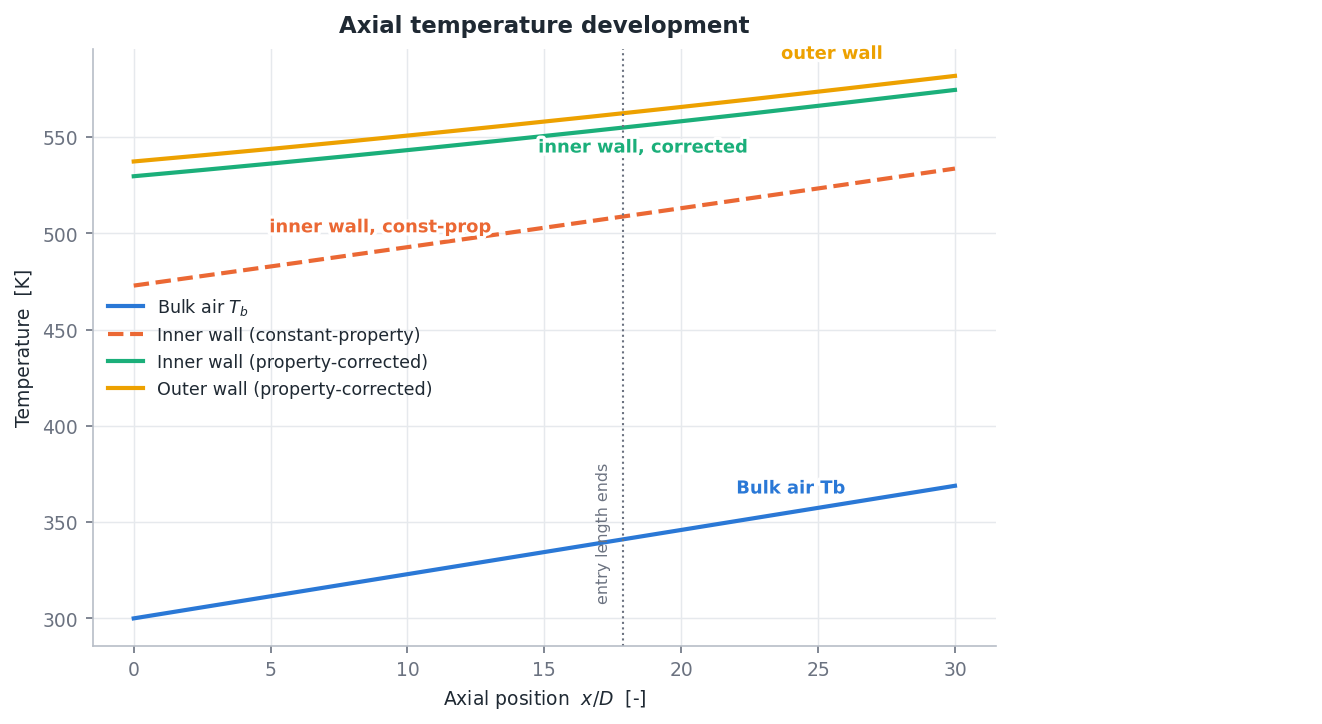
\includegraphics[width=\linewidth]{01_axial_temperatures.png}\caption{Axial temperature development}\end{subfigure}\hfill
\begin{subfigure}[t]{0.31\linewidth}\centering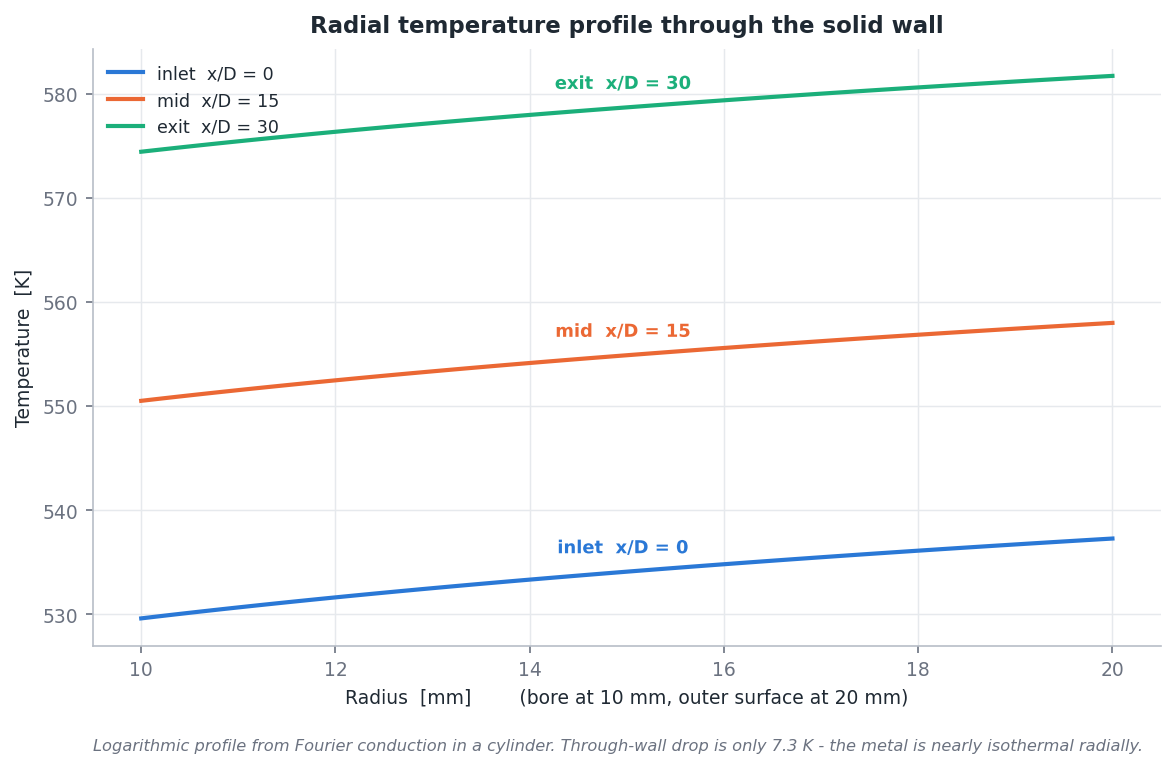
\includegraphics[width=\linewidth]{03_radial_wall_temperature.png}\caption{Radial wall temperature}\end{subfigure}\hfill
\begin{subfigure}[t]{0.31\linewidth}\centering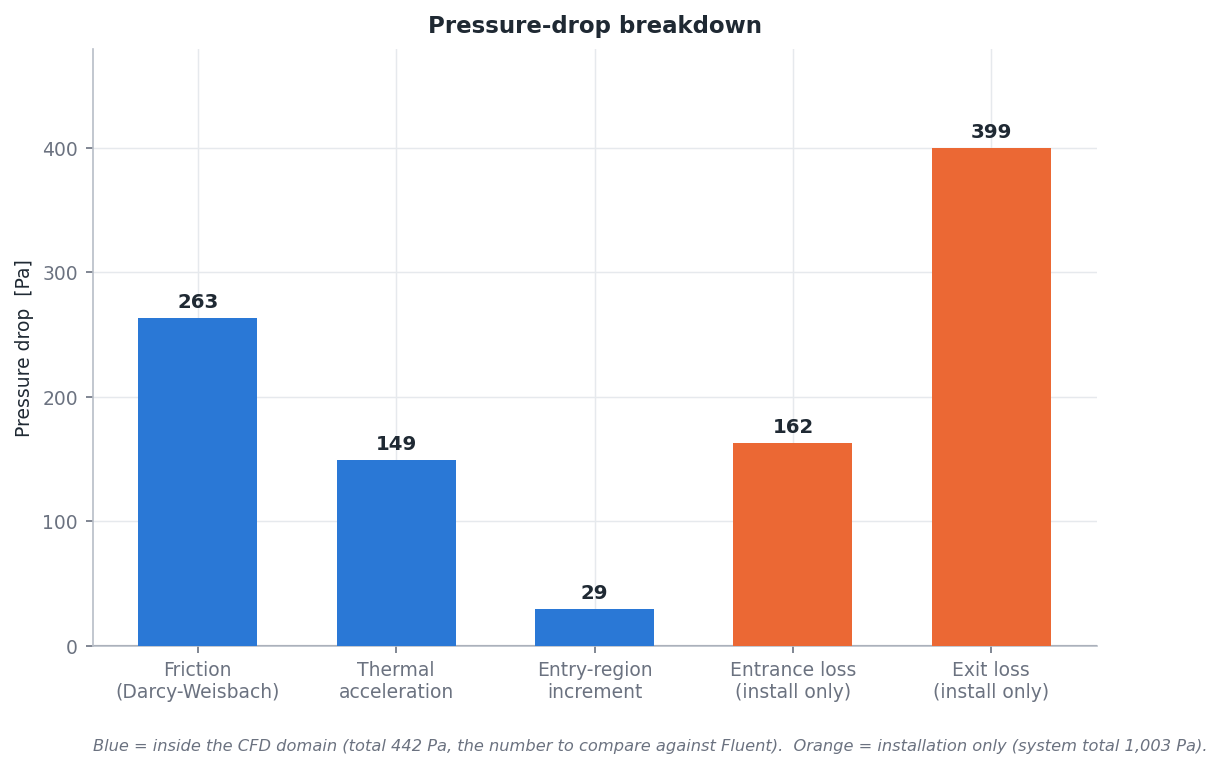
\includegraphics[width=\linewidth]{05_pressure_breakdown.png}\caption{Pressure-drop breakdown [Pa]}\end{subfigure}
\caption{Section 2 analytical baseline plots (ANALYTICAL level, produced before any CFD run).}
\label{fig:anplots}
\src{Source: \texttt{02\_Engineering\_Calculations/calculation\_plots/}; matplotlib plots of the analytical model.}
\end{figure}

\chapter{Mesh Tables}\label{app:mesh}
The CFD mesh family is defined in Tables~\ref{tab:meshfam} and~\ref{tab:meshq} and the structural mesh variants in Table~\ref{tab:smesh}.
On the coarse, medium and fine CFD meshes $y^+_{max}$ is 0.522, 0.585 and 0.653, always in the first slab, with 100\,\% of the wall at $y^+ \le 1$.

\chapter{CFD Monitor and Convergence Data}\label{app:conv}
The convergence criteria and final residuals are in Table~\ref{tab:convcrit} and the history in Figure~\ref{fig:conv}. The evaluation at
iteration 400 was not possible (too few second-order iterations), 500 was refused (scheme-switch transient), 600 met every criterion and
700 confirmed it. The fluid stayed within 299.998--553.42~K and the solid within 300.0--562.133~K throughout, inside both property tables,
with no limiter, divergence or reversed-flow message. All other CFD cases used the same staging and criteria.

\chapter{Structural Results}\label{app:struct}
The main static results are in Table~\ref{tab:lcres} and the first-yield assessment in Table~\ref{tab:yield}. Table~\ref{tab:appE} adds the
equilibrium and consistency checks. Stress singularities were checked on mesh B: averaged and unaveraged peaks differ by 0.30\,\% (LC1) and
0.004\,\% (LC2), and the energy-norm error is concentrated in the first 15~mm. An independent verification script re-derived the static results
from the raw MAPDL tables.

%% generated by gen_tables.py - RE-ANALYSIS 2026
\begin{table}[htbp]
\centering
\footnotesize
\caption{Additional structural results of the baseline}
\label{tab:appE}
\begin{tabular}{>{\raggedright\arraybackslash}p{0.55\linewidth}r}
\toprule
Quantity & Value \\
\midrule
LC1 reaction resultant [N] & $9.0\times10^{-7}$ \\
LC2 end reactions balanced to [N] & $1.8\times10^{-8}$ \\
LC2 reaction vs analytical restrained force of the same field & agreement to $10^{-5}$ \\
LC2 interior von Mises [MPa] & 587--591 \\
LC2 axial stress at mid-span, outer / bore [MPa] & $-$593.4 / $-$564.9 \\
LC2 maximum radial displacement [mm] & 0.0897 \\
LC1 free growth vs independent $\int\varepsilon_{th}\,dz$ & agreement to $1.3\times10^{-5}$ \\
LC2P peak von Mises [MPa] & 605.160918 \\
LC2 peak von Mises [MPa] (same precision) & 605.160873 \\
Energy-norm error LC1 / LC2 & 0.70\,\% / 0.012\,\% \\
\bottomrule
\end{tabular}
\par\smallskip\parbox{\linewidth}{\footnotesize\raggedright Source: \texttt{08\_Structural\_Analysis/STRUCTURAL\_RESULTS.md}, \texttt{PROJECT\_STATE.md} \S14.1, \texttt{FINAL\_ENGINEERING\_AUDIT.md} \S10.}
\end{table}


\chapter{Buckling Results}\label{app:buckling}
The hand estimates are in Table~\ref{tab:section}, the FE baseline results in Table~\ref{tab:buckling} and the support scenarios in
Table~\ref{tab:support}. Table~\ref{tab:appF} lists the first eigenvalue on every structural mesh. The workflow was benchmarked on a
constant-property toy tube: the Section 8A benchmark reproduced the closed-form Euler loads for the guided and no-sway end conditions, and
benchmark B03 gave a $\lambda_1$ between the plain and shear-corrected fixed--pinned values for the S3 remote-point formulation.

%% generated by gen_tables.py - RE-ANALYSIS 2026
\begin{table}[htbp]
\centering
\footnotesize
\caption{First eigenvalue on every structural mesh (S1 supports)}
\label{tab:appF}
\begin{tabular}{lrr}
\toprule
Mesh & Nodes & $\lambda_1$ (7 digits) \\
\midrule
XC & 24,171 & 1.1079876 \\
C & 50,652 & 1.1080342 \\
B (baseline) & 108,252 & 1.1080471 \\
FR & 127,080 & 1.1080404 \\
FA & 126,468 & 1.1080483 \\
FC & 126,294 & 1.1080410 \\
\bottomrule
\end{tabular}
\par\smallskip\parbox{\linewidth}{\footnotesize\raggedright Source: \texttt{PROJECT\_STATE.md} \S16.1 and \texttt{BUCKLING\_MESH\_COMPARISON.md}. Family monotonic (apparent order 4.9, GCI $5.6\times10^{-6}$); fine meshes within $6\times10^{-6}$ of B; $P_{cr}$ = 608.22--608.25 kN on all meshes.}
\end{table}


\chapter{Parametric Tables}\label{app:param}
The parametric results are in Tables~\ref{tab:pcfd}, \ref{tab:pstruct}, \ref{tab:pbk} and~\ref{tab:psens}; the changes from P00 are discussed in
Chapter~\ref{ch:param}, and the machine-readable tables are in the project folder \texttt{10\_Parametric\_Study}. The independent verification
\texttt{verify\_9B2.py} passed 45 of 46 checks; the single failure is the thickness check-mesh tolerance noted in Chapter~\ref{ch:unc},
reported rather than relaxed.

\chapter{Traceability}\label{app:trace}
\textbf{Status of the work.} The note on the analysis record at the front of the report applies to every value; only the engineer,
programme, organisation, period and tool set are documented internship facts.

\textbf{Numbers.} Every result value in the tables is read by \texttt{gen\_tables.py} from the Section 10A master dataset
\texttt{11\_Final\_Audit/MASTER\_PROJECT\_DATA.csv}: of its 182 rows, 124 are VERIFIED (recomputed from the raw solver or report file),
3 CROSS-CHECKED, 29 REPORTED (post-processing quantities from the section result files), 20 INPUT, 2 DECISION and 4 INTERPRETATION, and none
is a MISMATCH. Other values (solver settings, mesh controls, property tables) are quoted from the section documents named in each table note.
\texttt{qc\_10B.py} traces every number of the report to the master dataset or a project document (\texttt{Final\_Report/REPORT\_QC\_CHECKLIST.md}).

\textbf{Modelling levels and figures.} 581.7~K (analytical), 562.58~K (CFD medium) and 560.83~K (CFD fine), or $-$657.2~MPa (analytical
restrained stress) and 605.16~MPa (FE peak von Mises), belong to different modelling levels: they are different models or quantities, not
contradictions. All figures are hash-verified project files (\texttt{Figures/figure\_sources.json}); none is an ANSYS GUI screenshot.

\end{document}
